% !TEX program = xelatex
\documentclass[10pt]{article}
\usepackage[UTF8]{ctex}
\usepackage[utf8]{inputenc}
\usepackage[T1]{fontenc}
\usepackage{amsmath}
\usepackage{amsfonts}
\usepackage{amssymb}
\usepackage[version=4]{mhchem}
\usepackage{stmaryrd}
\usepackage{graphicx}
\usepackage[export]{adjustbox}
\graphicspath{ {./images/} }
\usepackage{hyperref}
\usepackage{wrapfig}
\hypersetup{colorlinks=true, linkcolor=blue, filecolor=magenta, urlcolor=cyan,}
\urlstyle{same}

\title{How to write a good scientific paper - Chris A. Mark}

\date{}


% %New command to display footnote whose markers will always be hidden
% \let\svthefootnote\thefootnote
% \newcommand\blfootnotetext[1]{%
%   \let\thefootnote\relax\footnote{#1}%
%   \addtocounter{footnote}{-1}%
%   \let\thefootnote\svthefootnote%
% }

% %Overriding the \footnotetext command to hide the marker if its value is `0`
% \let\svfootnotetext\footnotetext
% \renewcommand\footnotetext[2][?]{%
%   \if\relax#1\relax%
%     \ifnum\value{footnote}=0\blfootnotetext{#2}\else\svfootnotetext{#2}\fi%
%   \else%
%     \if?#1\ifnum\value{footnote}=0\blfootnotetext{#2}\else\svfootnotetext{#2}\fi%
%     \else\svfootnotetext[#1]{#2}\fi%
%   \fi
% }

\begin{document}
\maketitle


% 横线+无缩进段落
\newcommand{\myfootnote}[1]{
{\noindent\rule{5cm}{0.4pt}}\\
{\setlength\parindent{0pt}#1}
}

\section*{前言}

% Writing for peer-reviewed publication is an important part of the careers of many scientists and engineers. It is also an essential part of the scientific enterprise. Something this important should be done well. However, many scientists and engineers do not consider themselves good writers, so how can the average scientist write a good scientific paper?
为同行评审的出版物撰写文章是许多科学家和工程师职业生涯的重要组成部分。这也是科学事业不可或缺的一部分。如此重要的事情应该做好。然而,许多科学家和工程师并不认为自己是优秀的作家,那么普通科学家如何能撰写一篇优秀的科学论文呢?

% The good news is you do not have to be a good writer to write a good science paper, but you do have to be a careful writer. And while the creativity that often marks good science will sometimes spill over into the writing about that science, in general, good science writing does not require creative writing. In particular, writing for a peer-reviewed science or engineering journal requires learning and executing a specific formula for presenting scientific work.
好消息是,你不需要成为一名优秀的作家就能写出一篇好的科学论文,但你必须成为一名细心的作者。虽然通常标志着良好科学的创造力有时会渗透到关于该科学的写作中,但总体而言,好的科学写作并不需要创造性写作。特别是,为同行评审的科学或工程期刊撰写文章需要学习和执行一个特定的公式来展示科学工作。

% This book is all about teaching the style and conventions of writing for a peerreviewed science journal. (For the sake of brevity, I will use the word "science" to mean both science and engineering.) Anyone who absorbs the lessons of this book can become a better writer. At the least, you can become a good enough writer that your readers will judge your work by the quality of the science rather than the quality of the writing.
这本书完全是为了教授在同行评审的科学研究期刊中写作的风格和规范。(为了简洁起见,我将使用“科学”一词来指代科学和工程。)任何吸收了这本书教训的人都能成为一个更好的写作者。至少,你可以成为一个足够好的写作者,让读者根据你研究的质量而非写作质量来评判你的工作。

% What I know about science writing has come from three separate experiences. First, I have written over 200 papers in my $30+$-year career in the semiconductor industry. Like most authors, I have become a better writer through practice. I have also spent the last six years as Editor-in-Chief of the Journal of Micro/Nanolithography, MEMS, and MOEMS $\left(\mathrm{JM}^{3}\right)$, published by SPIE. That experience has forced me to judge the writing of others and to see the good, the bad, and the ugly of science publishing. Because of this experience, I embarked on a project of studying what makes for good science writing, and I have read many papers and books by other writers, editors, and historians of science on that topic. Taking advantage of my post as Editor-in-Chief, I started writing a series of editorials in $\mathrm{JM}^{3}$ on good science writing (2012-2018). This book is mostly a compilation of those editorials.
我对科学写作的了解来自三个不同的经历。首先,在我超过30年以上的半导体行业职业生涯中,我撰写了200多篇论文。像大多数作者一样,我通过实践成为了一个更好的写作者。在过去六年里,我还担任了《微/纳米光刻、微电子机械系统与微光学期刊》(Journal of Micro/Nanolithography, MEMS, and MOEMS,简称JM\textsuperscript{3})的主编,该期刊由SPIE出版社出版。那段经历迫使我去评判他人的写作,并见证了科学出版界的优点、不足和丑陋之处。由于这段经历,我着手研究什么构成了好的科学写作,并阅读了许多其他作家、编辑和科学史学家的论文和书籍。利用我作为主编的身份,我开始在JM\textsuperscript{3}上发表一系列关于良好科学写作的社论(2012-2018年)。这本书主要是那些社论的汇编。

% \section*{The Three Pillars of Science}
\section*{科学三大支柱}
% Science can be thought of as the combination of three essential things: (1) a communal collection of knowledge (both facts/data and theories); (2) a method of evaluating the efficacy of scientific theories by comparing the predictions of those theories to observation/experiment; and (3) an attitude of skeptical inquiry and the belief that all scientific knowledge is provisional and subject to revision when confronted with new evidence. (A popular alternative breakdown of the "norms" of science, emphasizing its sociological nature, is Merton's "cudos", first introduced in 1942: communalism, universality, disinterestedness, originality, and skepticism. ${ }^{1}$ ) This breakdown of science into a body of knowledge, a method, and an attitude is useful in assessing the "scientific" content of any given behavior. If any one of these three pillars of science is missing from an activity, one cannot claim that the activity is scientific.
科学可以被看作是三者的结合:(1)一个共同的知识集合(包括事实/数据以及理论);(2)一种通过将理论预测与观察/实验结果进行比较来评估科学理论有效性的方法;(3)一种怀疑性的探究态度,并相信所有科学知识在遇到新证据时都是临时的,并有待修订。(一个流行的将科学的“规范”分解为强调其社会学性质的方法是默顿在1942年首次提出的“科学规范”:共有性、普遍性、无私性、原创性和怀疑性。${ }^{1}$ )将科学分解为知识体系、方法和态度,这对于评估任何特定行为的“科学”内容是有用的。如果从一项活动中缺少了这三个科学支柱中的任何一个,那么人们不能声称这项活动是科学的。

\begin{wrapfigure}{r}{0.3\textwidth}
    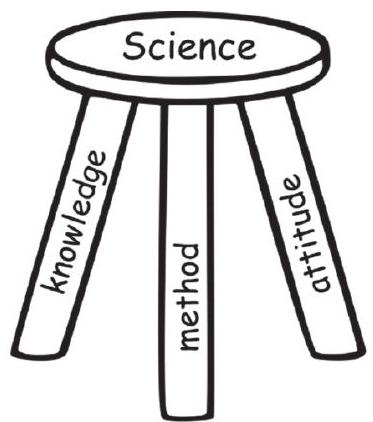
\includegraphics[width=0.28\textwidth, center]{2024_04_11_419211c3e451fc7cea07g-002}
    \end{wrapfigure}

% The growth of scientific knowledge is
科学知识的增长是
% predominately incremental — we build on past knowledge more often than we displace it. Thus, the first pillar of science-a communal collection of knowledge-requires mechanisms for disseminating and preserving knowledge within the scientific community. By far the most important mechanism in use today is the scientific publication. Although there are many forms of scientific publication, the most important is the peer-reviewed journal paper. The goal of this book is to help authors produce good scientific papers and thus support the goals of science.
主要以增量方式进行——我们更多地是在过去知识的基础上进行构建,而不是替换它。因此,科学的第一大支柱——共同的知识集合——需要机制在科学界内传播和保存知识。到目前为止,今天使用最重要的机制就是科学出版物。尽管科学出版物有许多形式,但最重要的还是同行评审的期刊论文。这本书的目标是帮助作者撰写优秀的科学论文,从而支持科学的目标。

% \section*{Using This Book}
\section*{使用这本书}
% This book can be read straight through, which I recommend for early-career scientists who are relatively new to writing and publishing papers. It can also be used as a reference for specific topics (e.g., how to produce a good figure or write an abstract). Each chapter is purposely short and can be read in isolation for easy reference. The appendix - a checklist for editors, reviewers, and authors - is a summary of the lessons of this book.
这本书可以一气呵成地阅读,我建议初入职业生涯的科学家们,尤其是那些在撰写和发表论文方面相对较新的人这样做。它也可以作为特定主题的参考资料(例如,如何制作优质的图表或撰写摘要)。每个章节都特意保持简短,可以单独阅读以便于查阅。附录部分——为编辑、审稿人和作者准备的清单——是对本书教训的总结。

% Throughout this book I will use the words "science" and "scientist" in the most expansive way possible to include people and activities generally called "engineering." Publishing in highly practical engineering fields or highly theoretical science fields (and every part of the continuum in between) has mostly the same requirements. Some fields, such as medicine, include additional important requirements, especially related to the use of and reporting on human or animal subjects. I will not be covering those important topics in this book, but the general lessons here apply even to those more specialized fields.
在整本书中,我将尽可能广泛地使用“科学”和“科学家”这两个词,以包括通常被称为“工程”的人和活动。在高度实用的工程领域或高度理论性的科学领域(以及这两个领域之间的任何部分)出版,大多数情况下有相同的要求。一些领域,如医学,还包括额外的 重要要求,特别是与使用和报告人类或动物受试者相关的部分。我在这本书中不会涉及这些重要主题,但这里的一般性教训同样适用于那些更专业的领域。

% Because of my experience as Editor-in-Chief of $\mathrm{JM}^{3}$, I have intimate knowledge and insider information about this specific journal. Where useful, I have included specific information from $\mathrm{JM}^{3}$ to use as examples of the points  make in the book. $\mathrm{JM}^{3}$ is probably representative of journals positioned halfway between pure science and pure engineering, and I hope that examples from this journal will make the lessons of this book more real.
因为我在担任《JM\textsuperscript{3}》主编的经历,我对这本特定的期刊有着深入的了解和内部信息。在有用的情况下,我已从《JM\textsuperscript{3}》中摘录了具体信息,用作书中论点的实例。《JM\textsuperscript{3}》可能代表了介于纯科学和纯工程之间的期刊,我希望这个期刊的例子能使本书的教学内容更加真实。

% \section*{Acknowledgments}
\section*{致谢}
% My learning about science writing leaves me with many debts of gratitude. The experience of writing, for me, had been a mostly joyful and satisfying one. I am indebted to the many good authors who I have read and to the many coauthors I have been privileged to write with. Less pleasant have been the rejection letters and difficult reviews that I have received over the years, but I am even more indebted to these editors and reviewers for their careful and constructive criticisms that forced me to improve even when I did not want to. I am also grateful for the readers of my books and articles who have given me feedback and asked me questions. They have taught me that when a reader does not understand what I have written, it is almost always my fault, not theirs.
我对科学写作的学习让我欠下了许多感激之情。对我来说,写作的经历大多是快乐和令人满足的。我感激那些我阅读过的许多优秀作者,也感激那些我有幸与之合作的许多合著者。不太愉快的是多年来我收到的拒稿信和艰难的评审意见,但我甚至更感激这些编辑和评审人员,他们的仔细和建设性的批评迫使我在即使不想改进的时候也要提升自己。我还感谢我的书籍和文章的读者们给予我的反馈和提问。他们教会了我,当读者不理解我所写的内容时,几乎总是我的错,而不是他们的。

% I would also like to thank the volunteer scientists that make up the editorial board of $\mathrm{JM}^{3}$. Together, we have gone through the sometimes exciting but often routine process of publishing a peer-reviewed science journal issue after issue. Finally, I would like to thank the wonderful staff of SPIE, who not only publish $\mathrm{JM}^{3}$ but are also publishing this book and making it freely available in electronic format. I have learned a tremendous amount from Eric Pepper and Karolyn Labes, who have coached and mentored me in my role as Editor-in-Chief and have reviewed and improved all of the material in this book. Thanks to John Mays and Scott McNeill as well for reviewing the text of this book.
我还想感谢组成《 JM\textsuperscript{3} 》编辑部的志愿者科学家们。我们一起经历了有时令人兴奋但通常却是常规的同行评审科学期刊出版过程,一期又一期。最后,我想感谢SPIE的优秀员工,他们不仅出版了《 JM\textsuperscript{3} 》,还出版了这本书,并将其以电子格式免费提供。我从Eric Pepper和Karolyn Labes那里学到了大量的知识,他们在我担任总编辑的角色中给予了我指导与辅导,并审查和改进了这本书中的所有材料。同时也要感谢John Mays和Scott McNeill对这本书的文本进行了审阅。

% I conclude with these oft-repeated words: much of what is good in this book is a consequence of the many people who have helped me over the years, and all of what is bad is due to my own shortcomings.
我以这些常常重复的话作结:这本书中所有的好处,都是多年来帮助过我的许多人的成果;而所有的不足,都是我个人的缺点造成的。

Chris A. Mack

Austin, Texas

January 2018


% \section*{References}
\section*{参考文献}


\myfootnote{${ }^{1}$ R. K. Merton, The Sociology of Science: Theoretical and Empirical Investigations, University of Chicago Press, Chicago, IL (1973).
}
% \section*{Chapter 1}
\section*{第一章}
% \section*{Getting Started}
\section*{开始入门}
% If you are thinking about writing a science paper for peer review and publication, what should be your first steps? Ideally, you have thought about the possibility of writing and publishing early in your research project because some early planning can help you avoid problems later. But first, you should ask yourself about your motivations for writing a science paper.
如果你在考虑撰写一篇科学论文以供同行评审和发表,你的第一步应该是什么?理想情况下,你应该在研究项目早期就考虑写作和发表的可能性,因为一些早期的规划可以帮助你后期避免问题。但首先,你应该问自己,你撰写科学论文的动机是什么?

% \subsection*{1.1 Why Write and Publish a Paper?}
\subsection*{1.1 为什么要撰写并发表论文?}
% Writing a paper and getting it published in a peer-reviewed journal is hard work, even after the hard work that led to the publishable results. So why do people do it? What motivates authors to go through the writing process, and then the peer review process, in order to publish their work? There are two kinds of motivations, altruism and self-interest, and most authors have some combination of the two.
在同行评审期刊上发表一篇论文是艰苦的工作,即使是在得出可发表结果之前的辛勤工作之后。那么人们为什么会这么做呢?是什么激励作者经历写作过程,然后再经历同行评审过程,以发表他们的作品呢?有两种类型的动机,即利他和自我利益,大多数作者都有这两种动机的组合。

% \section*{Altruism}
\section*{利他主义}
% Peer-reviewed science publications are the predominant method today for disseminating and archiving scientific advances (books, conference presentations, and university teaching are other common ways). Science grows and advances through a communal collection of knowledge that is constantly being challenged, revised, and expanded. ${ }^{1,2}$ Most scientists (and I include engineering in the broadest sense of science) have a strong desire to contribute to the advancement of their field, which is often their primary reason for becoming a scientist. Publication is usually the most straightforward way to make such a contribution, and it is thus highly motivating (and satisfying) to most scientists.
同行评审的科学出版物是目前传播和归档科学进展的主要方式(书籍、会议报告和大学教学是其他常见方式)。科学通过一个不断受到挑战、修订和扩展的集体知识库不断发展进步.${ }^{1,2}$ 大多数科学家(我将在最广泛的意义上包含工程)都有强烈的愿望为他们的领域做出贡献,这往往是他们成为科学家的主要原因。发表文章通常是作出这种贡献最直接的方式,因此对大多数科学家来说是非常激励人心(且令人满意)的。

% \section*{Self-Interest}
\section*{自我利益}
% Publishing can also bring tangible benefits to an author, thus providing a selfinterested motivation for writing and publishing a paper. Publishing may be required for career advancement and is frequently accompanied by direct or indirect monetary rewards. The familiar "publish or perish" paradigm in academia adds a proverbial stick to the carrot of career advancement. But even without these obvious professional motivations, almost all human beings crave recognition for their efforts. I know that I am highly motivated by the reward of peer recognition;
出版也能给作者带来实际利益,因此为撰写和发表论文提供了自我利益的动机。出版可能被视为职业发展的必要条件,并且常常伴随着直接或间接的金钱奖励。学术界熟悉的“不发表就消亡”的范式,为职业晋升的胡萝卜加大棒增添了谚语式的压力。但即使没有这些明显的职业动机,几乎所有人都会渴望他们努力的认可。我知道我自己就非常受同伴认可的奖励所激励。

% I am gratified to see my worked used and referenced, and I take pride in publishing in journals that I respect and admire.
我很欣慰能看到我的工作被使用和引用,我为能在自己尊敬和仰慕的期刊上发表作品感到自豪。

% \section*{Balancing Altruism and Self-Interest}
\section*{平衡利他主义与自我利益}
% Let me be clear that I do not view self-interested motivations as inherently bad or even fundamentally worse than altruistic motivations. Any properly regulated and well-functioning "marketplace" (to borrow economic parlance) aligns selfinterested and selfless motivations as much as possible. I suspect that every author has some combination of these two classes of motivation. The problem comes when altruism and self-interest are not balanced. In particular, if self-interest becomes so strong as to become selfish and swamp the altruistic goal of scientific advancement, the entire scientific enterprise can suffer.
让我明确一点,我并不认为自私的动机本质上是坏的,甚至不一定比利他的动机根本要差。任何适当规范和运作良好的“市场”(借用经济术语)都会尽可能地将自私和无私的动机相协调。我怀疑每个作者都有这两种类型动机的结合。问题在于当利他和自私的动机不平衡时。特别是,如果自私的动机变得如此强烈以至于变得自私自利,淹没了科学进步的利他目标时,整个科学事业都可能受到影响。

% In the academic world, as in the economic world, systems that promote greater disparity in "wealth" contribute to unbalanced selfishness. A winner-take-all tournament, where only the scientists with the top-rated papers published in the top-rated journals have a chance of getting jobs, tenure, grants, and students, will skew motivations towards self-interest. In the business world, rewarding and recognizing only monetary gain for one's employer can have the same effect. (Some universities are actively applying both pressures to their professors.) The result can be a continuum of sins: lack of motivation for replication experiments, ${ }^{3}$ bias against the null result, increased prevalence of faddish and safe science over creative exploration, unnecessary feuds over priority, preference for competition over collaboration ${ }^{4}$ lack of transparency and full disclosure, conflicts of interest, double publication, plagiarism, and outright fraud. (Many of these subjects will be discussed in the following chapters.)
在学术界,正如在经济领域,那些促进“财富”更大不平等的体制将导致不平衡的自私行为。一个赢者通吃的竞赛,只有那些在顶级期刊上发表顶级论文的科学家才有机会获得工作、终身职位、资助和学生,这将使动机偏向于个人利益。在商业界,只奖励和认可为雇主带来金钱收益的行为可能产生同样的效果。(一些大学正在积极对教授施加这两种压力。)其结果可能是一系列罪行的连续:缺乏复制实验的动力,对零结果的反向偏见,时尚且安全的研究比创造性探索更为普遍,不必要的优先权争夺,竞争偏好于合作,缺乏透明度和完全公开,利益冲突,双重发表,剽窃,以及公然的欺诈行为。(以下章节将讨论其中的许多主题。)

% With the exception of outright fraud (at least, to my knowledge), the Journal of Micro/Nanolithography, MEMS, and MOEMS $\left(\mathrm{JM}^{3}\right)$ has seen all of these sins in manuscripts submitted for publication during my tenure as editor-in-chief. I have no idea if any of these imbalances are trending up or down today. I do know that the best way to combat imbalanced self-interest is to find ways to constantly remind yourself of why you became a scientist or engineer in the first place: to make a positive difference in the world. (Am I being too bold or naïve to make this assumption about each of you? I do not think so.) If you keep your altruistic motivations always close and never compromised, the personal benefits can come along (self-interest "and" altruism, rather than "or").
除了公然的欺诈(至少在我所知范围内),在我担任《微纳米光刻、MEMS和MOEMS杂志》(JM3)主编期间,该杂志在提交出版的手稿中看到了所有这些弊端。我不知道如今这些不平衡是否在上升或下降。但我知道,对抗失衡的自私利益的最好方法就是找到不断提醒自己为何成为一名科学家或工程师的方式:为了在世界上产生积极影响。(我这样假设你们每一个人是否太大胆或太天真了?我不这么认为。)如果你始终怀揣着利他的动机,并且永不妥协,那么个人利益自然会随之而来(是“利己和利他”,而不是“利己或利他”)。

% \subsection*{1.2 The Literature Search}
\subsection*{1.2 文献检索}
% A new research project almost always begins with a literature search — or at least it should. The goal of the search is to evaluate the state of our communal knowledge on a topic before embarking on a quest of adding to that knowledge. Because science is about either confirming or refuting existing knowledge or developing new knowledge, a thorough understanding of the current state of communal knowledge is essential. Additionally, this literature search will form  foundation for the five goals of citations (see Chapter 5). Note that a literature search is not about finding relevant papers, it is about reading relevant papers.
一个新的研究项目几乎总是从文献检索开始的——或者至少应该是这样。检索的目的是在着手增加我们的集体知识之前,评估一下我们对某个话题的集体知识状态。因为科学要么是证实或反驳现有知识,要么是发展新知识,对集体知识当前状态的彻底理解是至关重要的。此外,这次文献检索将为引用的五个目标(见第5章)奠定基础。请注意,文献检索不仅仅是寻找相关的论文,更重要的是阅读这些相关论文。

% Unfortunately, literature searches are rarely done as well as they should be. Here are a few hints to improve literature searches:
不幸的是,文献搜索很少能做到应该做到的那样好。以下是一些建议,可以帮助改进文献搜索:

\begin{itemize}
%   \item Do the literature search before performing the research, and certainly before writing the paper.
\item 在进行研究之前进行文献搜索,当然在写论文之前也要做。
%   \item The next most promising papers to read are often those referenced in the relevant papers you have already found.
\item 接下来最值得一读的论文往往是那些你已经找到的相关论文中所引用的。
%   \item Look in fields outside your discipline (this often means looking for different search keywords, which one recursively discovers when reading the literature outside of one's discipline).
\item 看看你专业领域以外的领域(这通常意味着要寻找不同的搜索关键词,而这些关键词是当你阅读自己专业领域以外的文献时递归发现的)。
%   \item While your memory of which previous papers are worth citing is a good start, no one ever knows the full scope of the literature in even the smallest of niche fields. Do not rely on your memory alone.
\item 虽然你记得哪些以前的论文值得引用是一个不错的开始,但即便是小众领域,也没有人能够完全了解文献的全貌。不要仅依靠你的记忆。
%   \item When finishing up the manuscript, look for recent publications on the subject. Often, other researchers are working on similar topics and may have published papers that should be read to ensure that your manuscript captures the latest communal knowledge in the field.
\item 在完成手稿时,要查找有关该主题的最新出版物。通常,其他研究人员可能正在研究类似的话题,并且可能已经发表了应该阅读的论文,以确保你的手稿能够捕捉到该领域最新的公共知识。
\end{itemize}

% Starting a literature search always leads to a difficult question: How do you know when to stop? There will always be important papers that you never find. This is the nature of modern science. Knowing when to quit (or pause) the literature search and begin the new work is a matter of judgment and experience.
开始文献搜索总是会导致一个困难的问题:你怎么知道什么时候该停止?总会有些重要的论文是你永远找不到的。这是现代科学的本质。知道何时停止(或暂停)文献搜索并开始新工作是关乎判断和经验的问题。

% \subsection*{1.3 Plan and Execute Research with Publication in Mind}
\subsection*{1.3 以发表为目的规划和执行研究计划}
% Most projects begin with the intention of writing a paper as an output of the work, or at least with the thought that this could be a possibility. If so, the research should be planned and executed with publication in mind. As discussed throughout this book (especially in Chapter 2), one of the critical requirements of a science paper is to document the work in sufficient detail so that the reader can follow the reasoning presented and validate the conclusions drawn. Furthermore, the authors of a published paper must be willing to defend the work against criticism, and so they should have available for later review the raw data used and significant detail about the experimental procedure.
大多数项目开始时都怀着写一篇论文作为工作成果的意图,或者至少考虑到这可能是一个可能性。如果是这样,研究就应该以发表为目标来进行规划和执行。正如本书全文所讨论的(尤其是在第2章中),科学论文的一个关键要求是详细记录工作,以便读者能够跟上所呈现的推理并验证得出的结论。此外,已发表论文的作者必须愿意为工作成果辩护,抵御批评,因此他们应该为后续审查保存所使用的原始数据和有关实验程序的详细信息。

% First and foremost, these goals require good laboratory record keeping. Classically, it is the "lab notebook" that has served this purpose, though today it is often a virtual notebook of (ideally) well-organized digital files. Knowing what you might need from these records for paper writing can help your record keeping. For example, if you review the requirements for what is needed in a method section of a paper (see Chapter 2), you will know what record keeping is required to make the process of writing the methods section easier.
首先,这些目标需要良好的实验室记录保持。传统上,起到这一作用的是“实验室笔记”,尽管在今天,这往往是一个(理想情况下)组织良好的数字文件的虚拟笔记。了解你在撰写论文时可能需要从这些记录中获取什么信息,可以帮助你进行记录保持。例如,如果你回顾一下论文方法部分所需的内容要求(见第2章),你就会知道需要哪些记录保持,以使撰写方法部分的过程更加容易。

% Raw data are often manipulated, reformatted, filtered, summarized, and graphed before being presented in a publication. It is almost always a requirement that the data be archived at each of these various stages. You do not want to be in a position of publishing a graph where the "picture" of the graph is the only thing that remains of the original data.
原始数据在发表前通常会被处理、重新格式化、筛选、汇总和制图。在这些各个阶段对数据进行归档几乎始终是必要的要求。你一定不想处于这样的境地:发布的图表中,图表的“图像”是原始数据的唯一遗留物。

% \subsection*{1.4 Conclusions}
\subsection*{1.4 结论}
% Experienced authors have a clear idea of what is required to write a good science paper, and so they plan and execute a research project with the requirements of publication in mind. For those with less experience, I recommend reading this book (especially Chapters 2, 7, and 12) at the beginning of a research project to make sure you can meet the most important requirements of writing and publishing your work.
经验丰富的作者对撰写优秀科学论文的要求有清晰的认识,因此他们会按照发表的要求来规划和执行研究项目。对于那些经验较少的人,我建议在研究项目开始时阅读这本书(尤其是第2、第7和第12章),以确保你能满足撰写和发表你作品的最重要要求。

% \section*{References}
\section*{参考文献}
\myfootnote{${ }^{1}$ R. K. Merton, The Sociology of Science: Theoretical and Empirical Investigations, University of Chicago Press, Chicago, IL (1973).

${ }^{2}$ T. S. Kuhn, The Structure of Scientific Revolutions, 3rd ed., University of Chicago Press, Chicago, IL (1996).

${ }^{3}$ Editorial, "Go forth and replicate!", Nature 536, 373 (2016).

${ }^{4}$ F. C. Fang and A. Casadevall, "Competitive Science: Is Competition Ruining Science?", Infection and Immunity 83(4), 1229 (2015).
}
% \section*{Chapter 2}
\section*{第二章}
% \section*{Structure and Organization}
\section*{结构和组织}
% Writing is inherently a creative process. That would seem a good fit for the science researcher, where creativity coupled with critical thinking is the key to success. Alas, many scientists do not think of themselves as qualified writers, finding the task of writing both intimidating and arduous. For those readers who are not already experienced at writing articles for scientific journals, I have a secret to share: you do not have to be a good writer to write a good scientific paper. The reason is this: there is a formula for how to structure and organize a scientific paper, so that the scientist/writer can focus on what they know best-the science- and worry less about the writing.
写作本质上是一个创造性过程。这对于科学研究人员来说似乎是一个很好的契合,因为创造力与批判性思维的结合是成功的关键。然而,遗憾的是,许多科学家并不认为自己是合格的作家,他们觉得写作这项任务既令人畏惧又艰巨。对于那些还没有为科学期刊撰写文章经验的读者,我有一个秘密要分享:你不必是一个优秀的作家才能写出一篇优秀的科学论文。原因在于:科学论文的结构和组织有一个公式,这样科学家/作者可以专注于他们最擅长的领域——科学——而不用太担心写作。

% A formula for writing may sound like a recipe for mediocrity, and in some contexts this would surely be true. But for the scientific paper, the emphasis must always stay on the science, with the words mere tools for effectively conveying information. Over the last 350 years, scientific journals have evolved a distinctive style, structure, and organization that make it easy for both the writer and the reader to get what they need from the paper: effective communication of scientific ideas.
写作的公式可能听起来像是平庸的处方,在某些情境中这确实是事实。但对于科学论文来说,重点必须始终放在科学上,文字仅仅是有效传达信息的工具。在过去的350年中,科学期刊已经形成了一种独特的风格、结构和组织方式,这使得作者和读者都能轻松地从论文中获得所需的内容:有效沟通科学思想。

% A major difference between journal-based science writing and the diverse forms of writing found elsewhere is the very limited scope of our medium. A scientific paper does not have to be all things to all people. It is a narrow genre with a narrow (though very important) purpose. A specific scientific community is not a random sampling of humanity but a group that shares an established and understood basic scientific background, a broadly agreed-upon set of common goals, and an already established set of mechanisms for the communication of information. By following the standard structure and organization of a science research article, the author is constrained in many respects. But these constraints free the author and the reader to focus on the content, which often results in a better paper.
期刊式科学写作与其它各种写作形式的一个主要区别在于我们媒介的范围非常有限。科学论文不必迎合所有人,它是一个范围狭窄(尽管非常重要)的文体。特定的科学社群并不是人类的随机样本,而是一个共享既定且理解的基本科学背景、广泛认同的共通目标,以及已经建立的信息交流机制的一群人。通过遵循科学研究文章的标准结构和组织,作者在许多方面受到限制。但这些限制让作者和读者可以专注于内容,这往往能导致一篇更好的论文。

% \subsection*{2.1 The Standard Structure of a Scientific Paper}
\subsection*{2.1 科学论文的标准结构}
% The vast majority of papers published in scientific journals today follow a fairly simple structure. With some variations, most papers use an "IMRaD" format:
当今发表在科学期刊上的绝大多数论文遵循一种相当简单的结构。在一些变体中,大多数论文使用“IMRaD”格式:

% This format is so ubiquitous that it is often surprising to see a paper that significantly deviates from it. (Outside of the field of science, this organizational model goes by the acronym CEC: claim, evidence, commentary.) Of course, there are many variations on this theme, and the structure is meant to advance the goal of communication, never hinder it. There are two main advantages of following the IMRaD structure: it makes it easier for the writer to organize the content of the paper, and it makes it easier for the reader to opportunistically find the information they seek. The following sections look at each of these standard sections in more detail.
这种格式如此普遍,以至于看到显著偏离它的论文常常会让人感到惊讶。(在科学领域之外,这种组织模型被称为缩写CEC:主张、证据、评论。)当然,这一主题有许多变体,结构旨在促进交流的目标,绝不应该妨碍交流。遵循IMRaD结构有两个主要优点:它让作者更容易组织论文内容,也让读者更容易有机会找到他们寻求的信息。以下各节将更详细地查看这些标准部分。

% \section*{2.2 Introduction }
\section*{2.2 引言}
% In standard rhetoric, the Introduction section should answer two questions: "What?" and "So what?" What is the paper about, and why should the reader care? The scientific journal paper is a specialized form of rhetoric, and so we use a more specialized format for our introduction, but answering these two questions is still required. Thus, an introduction should inform the reader as to what the paper is about and motivate the reader to continue reading.
在标准的修辞学中,引言部分应该回答两个问题:“是什么?”和“那又如何?”文章是关于什么的,读者为什么要在意?科学期刊论文是修辞学的一种特殊形式,因此我们在引言中使用了更为专业的格式,但回答这两个问题仍然是必须的。因此,引言应该告知读者文章是关于什么的,并激发读者继续阅读的兴趣。

% As will be discussed in Chapter 7, a paper must meet four criteria before it is publishable in a scientific journal:
正如第7章将要讨论的,一篇论文在发表在科学期刊之前,必须满足四个条件:

\begin{itemize}
%   \item The content of the paper must match the scope of the journal.
\item 论文的内容必须符合期刊的范围。
%   \item The quality of the paper (method and execution of the research, as well as the writing) must be sufficiently high.
\item 论文的质量(研究的方法和执行,以及写作)必须足够高。
%   \item It must present novel results (with the exception of review papers and the like).
\item 它必须呈现新颖的结果(回顾性论文等除外)。
%   \item The results must be significant enough to be worth reading (and thus worth publishing).
\item 结果必须足够重要,才值得阅读(也因此值得发表)。
\end{itemize}

% Of these four criteria, the author should clearly lay claim to three of these in the introduction (scope, novelty, and significance). Quality is implied and should be demonstrated, not explicitly claimed.
在这四个标准中,作者应该在引言中明确声明其中三个(范围、新颖性和重要性)。质量应该是暗示性的,并通过文章展现出来,而不是直接声明。

% The basic flow of the introduction starts with the general and then moves to the specific. As Swales has described it, the research-article introduction moves through three phases: ${ }^{1}$
引言的基本流程是从总体开始,然后转向具体。正如Swales所描述的,研究论文的引言分为三个阶段:${ }^{1}$

\begin{itemize}
%   \item Establish a territory (what is the field of the work, why is this field important, what has already been done?),
\item 建立领域(这项工作的领域是什么,这个领域为什么重要,已经完成了哪些工作?)
%   \item Establish a niche (indicate a gap, raise a question, or challenge prior work in this territory), and
\item 建立一个新的细分市场(指出这一领域中的空白,提出一个问题,或者挑战之前在这个领域的工作)。
%   \item Occupy that niche (outline the purpose and announce the present research; optionally summarize the results).
\item 占领那个市场缝隙(概述目的并宣布当前研究;可选择性总结结果)。
\end{itemize}

% An alternative formulation of these three parts of the introduction uses topic, problem, solution (for engineering); or topic, observation/discovery, explanation (for science). Some articles finish the introduction by presenting an outline of the article, although I am not a fan of this style. The section headings themselves are more effective than creating a table of contents in prose form.
这三部分引言的另一种表述方式是:主题、问题、解决方案(针对工程学科);或主题、观察/发现、解释(针对科学学科)。有些文章通过呈现文章大纲来完成引言部分,尽管我个人不太喜欢这种风格。实际上,章节标题本身比以散文形式创建目录更为有效。

% Some common pitfalls in writing an introduction include providing unnecessary background information (telling the reader what they already know or what they do not need to know), exaggerating the importance of the work, or failing to make clear what research questions this paper is trying to answer.
在撰写 引言时常见的陷阱包括提供不必要的背景信息(告诉读者他们已经知道或不需要知道的内容),夸大工作的重要性,或者未能明确指出这篇论文试图回答哪些研究问题。

% \subsection*{2.3 Method}
\subsection*{2.3 方法}
% The Method section (sometimes called the Materials and Method section) describes how the results were generated. It should be sufficiently detailed so that an independent researcher working in the same field could reproduce the results sufficiently to allow validation of the conclusions. Often, this does not require explicit step-by-step instructions but rather references to prior publications that provide such details. For some research articles, it is the method that is novel. For this case, a much more detailed description is required. For standard or wellestablished methods, naming the method may be sufficient.
方法部分(有时称为材料与方法部分)描述了结果是如何产生的。它应该足够详细,以便在同一领域工作的独立研究人员能够充分复现结果,以允许对结论进行验证。通常,这并不需要明确的逐步指导,而是参考提供这些细节的前期出版物。对于某些研究文章,新颖之处在于方法。在这种情况下,需要更详细的描述。对于标准或已确立的方法,命名该方法可能就足够了。

% Let us parse the requirement for "sufficient detail" a little more carefully. There are really two interrelated goals at work: the reader should be given the ability to reproduce the results and the ability to judge the results. ${ }^{2}$ Although very few readers attempt a replication of another's experiment, most careful readers attempt to judge the validity of the work they are reading. Internal validity means the conclusions drawn are supported by the results presented. External validity refers to the degree that the conclusions can be generalized (rather than being applicable only to the narrow confines of this one work). Without a carefully written method section, it becomes impossible to assess the validity of the work.
让我们更仔细地解析一下对“足够详细”的要求。这里实际上有两个相互关联的目标:一是读者应能够重现结果,二是读者应能够评判结果。${ }^{2}$尽管很少有读者尝试复制别人的实验,但大多数细心的读者会试图评判他们所阅读的作品的有效性。内部有效性指的是所提出的结论得到了呈现结果的支持。外部有效性指的是结论可以被推广的程度(而不是仅适用于这一篇狭隘的工作)。如果没有精心撰写的方法部分,就无法评估作品的有效性。

% A "method" is used here more broadly than an experimental method. The method can include the development of a theory (either as necessary background or as a novel element of the paper), the establishment of a specific device design, or the development or description of a modeling tool to be used. A common variation of the IMRaD structure separates the theory (or design or modeling) into its own preceding section before moving on to the experimental method.
在这里,“方法”一词被广泛地使用,不仅限于实验方法。该方法可以包括发展一个理论(作为必要的背景或作为论文的一个新颖元素)、建立一个特定的设备设计,或者是开发或描述一个将要使用的建模工具。IMRaD结构的一个常见变体是将理论(或设计或建模)单独分为一个在前面的部分,然后再继续介绍实验方法。

% A good method section should not only describe what was done and how it was done, but it should justify the experimental design as well. Of the many options available, why was this method chosen? Statistical considerations, such as sampling plans and analysis methods used, should be explained. If the raw results are not going to be presented, then a description of the data-reduction procedures is required. Also, consider how a figure or diagram might be used to illustrate or summarize the methods.
一个好的方法部分不仅要描述做了什么以及是如何做的,还应该证明实验设计的合理性。在众多可选方案中,为什么要选择这个方法?应该解释统计考虑因素,比如采用的抽样计划和分析方法。如果原始结果不会呈现,那么就需要描述数据简化程序的说明。此外,考虑如何使用图表或示意图来阐述或总结方法。

% A common shortcoming of method sections in many papers today is the abandonment of the goal of reproducibility. Usually citing economy as the driving principle, method sections are often overly brief and lacking in detail. Rarely does a method section explain why one approach was chosen over another. Nobody reproduces other people's work anymore, or so the thought goes. I find this attitude mistaken and often self-serving. Some researchers may not want their results to be reproduced, and more to the point, may not want the validity of their results to be questioned. Others may want to hide necessary details for commercial reasons. But the advancement of scientific knowledge requires both reproducibility and the ability to judge the quality and validity of published results. A thorough and detailed method section is the first and most important step in achieving these two goals.
当今许多论文中方法部分的一个常见不足是放弃了可重复性的目标。通常以经济性为原则,方法部分往往过于简短,缺乏细节。很少有一个方法部分会解释为什么选择一种方法而不是另一种。人们不再重复别人的工作了,这种想法似乎成了共识。我认为这种态度是错误的,往往是出于私心。一些研究人员可能不希望他们的结果被复制,更重要的是,可能不希望他们结果的有效性受到质疑。其他人可能出于商业原因想要隐藏必要细节。但是,科学知识的进步需要可重复性以及判断发表结果质量和有效性的能力。一个详尽且细致的方法部分是实现这两个目标的第一步,也是最重要的一步。

% Other common pitfalls when writing the Method section: including results in the Method section, including extraneous details (unnecessary to enable reproducibility or judge validity), or treating the method as a chronological history of what happened.
在撰写方法部分时其他常见的陷阱:在方法部分包含结果,加入无关细节(对可复制性或判断有效性并非必要),或者将方法当作是发生事件的编年史。

% \subsection*{2.4 Results and Discussion}
\subsection*{2.4 结果与讨论}
% The results of a paper, if included as its own section, should be very short. It is simply a presentation of the results obtained corresponding to the methods described in the previous section, organized to make them accessible to the reader. Often, these results are presented in tables and/or graphs. Well-crafted tables and figures require very little in terms of supporting text in the body of the paper (see Chapter 4), so the results are usually combined with a discussion of them in the results and discussion section. An important goal when presenting results is to clearly designate those results that are new (never before published), while properly citing results that have been previously published.
论文中的结果部分,如果单独作为一个章节,应该非常简短。它仅仅是展示与前一部分描述的方法相对应得到的结果,并通过组织使读者易于理解。通常,这些结果以表格和/或图表的形式呈现。精心制作的表格和图形在论文正文中需要的支持性文字很少(参见第4章),因此结果通常会与对它们的讨论合并到结果与讨论部分。在展示结果时,一个重要的目标是清晰地标明哪些结果是新的(以前从未发表过),同时适当地引用以前已经发表的结果。

% Evidence does not explain itself. The purpose of the Discussion section is to explain the results and show how they help to answer the research questions posed in the introduction. This discussion generally passes through the stages of summarizing the results, discussing whether results are expected or unexpected, comparing these results to previous work, interpreting and explaining the results (often by comparison to a theory or model), and hypothesizing about their generality. ${ }^{3}$
证据本身并不能解释自己。讨论部分的目的是解释结果,并展示它们如何帮助回答引言中提出的研究问题。这一讨论通常包括以下几个阶段:总结结果,讨论结果是预期内还是预期外的,将这些结果与之前的工作进行比较,解释和阐述结果(通常是通过与理论或模型的比较),以及对它们的普遍性进行假设。${ }^{3}$

% The Discussion section inverts the format of the introduction, moving from the specific (the results generated in this work) to the general (how these results demonstrate a general principle that is more widely applicable). Any problems or shortcomings encountered during the course of the work should also be discussed, especially if they might influence how results are to be interpreted.
讨论部分颠倒了引言的格式,从具体(本工作中产生的结果)到一般(这些结果如何展示一个更广泛适用的普遍原理)。在工作过程中遇到的任何问题或不足也应该进行讨论,特别是如果它们可能会影响结果的解释方式。

% Some common pitfalls when writing the results and discussion section are a lack of organization, presenting results that are never discussed, presenting discussion that does not relate to any of the results, presenting results and discussion in chronological order rather than logical order, ignoring results that do not support the conclusions, or drawing conclusions from results without sound logical arguments to back them up.
在撰写结果和讨论部分时,一些常见的陷阱包括组织混乱、呈现未被讨论的结果、讨论与任何结果无关的内容、按时间顺序而非逻辑顺序呈现结果和讨论、忽视不支持结论的结果,或者在没有坚实的逻辑论证支持的情况下从结果中得出结论。

% \subsection*{2.5 Conclusions}
\subsection*{2.5 结论}
% The Conclusions section provides a brief summary of the results and discussion, but it should be more than a summary. After showing how each research question posed in the introduction has been addressed, the implications of the findings should be emphasized, explaining how the work is significant. The goal here is to provide the most general claims that can be supported by the evidence. This section should be reader-focused, avoiding a list of all the things that "I" or "we" have accomplished.
结论部分提供了结果和讨论的简要概述,但它应不仅仅是一个总结。在展示了引言中提出的研究问题是如何得到解答之后,应该强调发现的含义,解释这项工作的重要性。这里的目的是提供可以通过证据支持的最一般的声明。这一部分应专注于读者,避免列出“我”或“我们”所完成的所有事项的清单。

% The Conclusions section should allow for opportunistic reading. When writing this section, imagine a reader who reads the introduction, skims through the figures, then jumps to the conclusion. The conclusion should concisely provide the key message(s) the author wishes to convey. It should not repeat the arguments made in the results and discussion, only the final and most general conclusions. While the results and discussion section is often quite long, the conclusion section is generally short.
结论部分应当便于机会性阅读。在撰写这一部分时,要想象一个读者在阅读了引言、快速浏览了图表之后,直接跳转到结论。结论应该简洁地提供作者希望传达的关键信息。它不应重复结果和讨论部分中的论点,只需给出最终和最一般的结论。尽管结果和讨论部分通常相当长,但结论部分一般较短。

% The second goal of the conclusion is to provide a future perspective on the work. This could be recommendations to the audience or a roadmap for future work. A small amount of speculation can be appropriate here, so long as it is relevant and clearly labeled as speculative.
结论的第二个目标是提供一个关于工作的未来视角。这可以是给读者的建议,也可以是未来工作的路线图。在这里可以进行一定程度的推测,只要它是相关的,并且明确标明为推测性质即可。

% Some common pitfalls when writing the conclusion are repeating the abstract, repeating background information from the introduction, introducing new evidence or new arguments not found in the results and discussion, repeating the arguments made in the results and discussion, or failing to address all of the research questions set out in the introduction. Because a conclusion should be more than just a summary, I prefer "Conclusions" as a title for this section over "Summary."
在撰写结论时,一些常见的误区包括重复摘要内容、重复引言中的背景信息、引入结果和讨论部分未出现的新证据或新论点、重复结果和讨论中提出的论点,或者未能解答引言中提出的所有研究问题。因为结论不应仅仅是一个总结,我更倾向于将这一部分的标题用“结论”而不是“摘要”。

% \subsection*{2.6 The Structures of Papers in the Journal of Micro/Nanolithography, MEMS, and MOEMS}
\subsection*{2.6 《微/纳米光刻、微机电系统及微光学电子期刊》中论文的结构安排}
% To explore whether the IMRaD structure is commonly used in my community, I examined the 100 papers published in the Journal of Micro/Nanolithography, MEMS, and MOEMS $\left(\mathrm{JM}^{3}\right)$ in 2013. I found that $78 \%$ of them employed some variation of the standard IMRaD organization. About half of these separated the theory from the Method section, which was the most common variant. Other variants included separating the motivation from the introduction, separating future work from conclusions, separating results from discussion, and dividing a long section (such as theory or discussion) into separate parts. Only one paper did not have an introduction section, and only one (different) paper did not have a conclusion section. The $22 \%$ that did not employ the IMRaD structure generally employed a structure that was more specific to that work, using descriptive headings that did not fall into the "methods" or "results and discussion" categories. One interesting structure created two parallel sets of sections, one for experiment and one for modeling.
为了探索IMRaD结构在我的社区中是否被普遍使用,我检查了2013年发表在《微/纳米光刻、MEMS和MOEMS杂志》(JM3)上的100篇论文。我发现其中有78%采用了标准IMRaD组织结构的一些变体。大约一半的论文将理论与方法部分分开,这是最常见的变体。其他变体包括将动机与引言分开,将未来工作与结论分开,将结果与讨论分开,以及将一个长部分(如理论或讨论)分成单独的部分。只有一篇论文没有引言部分,另一篇(不同的)论文没有结论部分。没有采用IMRaD结构的22%的论文通常采用了更具体于该工作的结构,使用的描述性标题不属于“方法”或“结果与讨论”类别。一个有趣的结构创建了两套平行的部分,一套用于实验,另一套用于建模。

% Headings and subheadings are an important part of a paper's organization. Headings are almost always required in science journals, but subheadings are often optional. Still, $88 \%$ of $\mathrm{JM}^{3}$ papers in 2013 used subheadings. About half $(49 \%)$ of the papers used generic headings (Introduction, Method, Results and Discussion, etc.), whereas the rest used substantive headings, changing the text of the heading to be specific to the topic of the paper. There are also optional sections found in many $\mathrm{JM}^{3}$ papers: $79 \%$ of the papers I looked at had an Acknowledgments section, and $5 \%$ had one or more appendices.
标题和副标题是论文组织的重要组成部分。在科学期刊中几乎总是要求使用标题,但副标题通常是可选的。然而,在2013年的JM3论文中,仍有88%使用了副标题。大约一半(49%)的论文使用了通用标题(引言、方法、结果与讨论等),而其余的则使用了实质性标题,即根据论文主题更改标题的文本。在许多JM3论文中还可以找到可选部分:我查看的论文中有79%包含了致谢部分,而5%的论文有一个或多个附录。

% \subsection*{2.7 Conclusions}
\subsection*{2.7 结论}
% (Let us see if I can follow my own advice about conclusions.)
(让我们看看我是否能遵循自己关于结论的建议。)

% Not everyone is good at writing, either by nature or inclination. For those of us who don't moonlight by writing articles for The New Yorker or Vanity Fair, writing a good scientific journal article is still within our grasp. One very helpful tool is to organize your paper according to the IMRaD model and follow the general advice listed earlier. Of course, if the nature of your work demands a different structure, feel free to change and invent. But most of the time, structuring your paper according to the standard organization most commonly used in science journals makes the writer's job easier and the reader's time more effective.
并非每个人都天生或倾向于擅长写作。对于那些不曾在《纽约客》或《名利场》兼职写作文章的我们来说,撰写一篇优秀的科学期刊文章仍然在我们的能力范围之内。一个非常有用的工具是按照IMRaD模型组织你的论文,并遵循前面列出的通用建议。当然,如果工作的性质要求不同的结构,可以随时进行改变和创新。但大多数时候,按照科学期刊中最常用的标准结构来安排你的论文,可以使作者的工作更轻松,也能更有效地利用读者的时间。

% \section*{References}
\section*{参考文献}
\myfootnote{${ }^{1}$ R. K. Merton, The Sociology of Science: Theoretical and Empirical Investigations, University of Chicago Press, Chicago, IL (1973).
}
\myfootnote{${ }^{1}$ R. K. Merton, The Sociology of Science: Theoretical and Empirical Investigations, University of Chicago Press, Chicago, IL (1973).

${ }^{2}$ T. S. Kuhn, The Structure of Scientific Revolutions, 3rd ed., University of Chicago Press, Chicago, IL (1996).

${ }^{3}$ Editorial, "Go forth and replicate!", Nature 536, 373 (2016).

${ }^{4}$ F. C. Fang and A. Casadevall, "Competitive Science: Is Competition Ruining Science?", Infection and Immunity 83(4), 1229 (2015).
}
\myfootnote{${ }^{1}$ J. M. Swales, Genre Analysis: English in Academic and Research Settings, pp. 140-166, Cambridge University Press, Cambridge, England (1990).

${ }^{2}$ L. F. Azevedo et al., "How to write a scientific paper - Writing the methods section", Rev. Port. Pneumol. 17(5), 232-238 (2011).

${ }^{3}$ J. M. Swales, Genre Analysis: English in Academic and Research Settings, 172-173, Cambridge University Press, Cambridge, England (1990).
}
% \section*{Chapter 3}
\section*{第三章}
% \section*{Language and Style}
\section*{语言与风格}
% "Have something to say, and say it as clearly as you can. That is the only secret of style."
“有话要说,尽可能清楚地表达出来。这就是风格的唯一秘诀。”

% \section*{- Matthew Arnold}
\section*{- 马修·阿诺德}
% Deserved or not, scientists and engineers have a reputation as bad writers. An average person reading a scientific journal paper will likely come away numb within a few sentences. Much of that is due to the complexity of the subject and a writing style that assumes a readership of knowledgeable peers. Some of that reputation is deserved, as many writers in our field either do not value clear and concise prose or do not know how to achieve it.
不论是否应得,科学家和工程师都有作为糟糕作家的名声。一个普通人在阅读科学期刊论文时,很可能在几句话之内就会感到麻木。这很大程度上是因为主题的复杂性和一种假定读者具备专业知识水平的写作风格。这种名声在一定程度上是应得的,因为在我们领域中,许多作者要么不重视清晰简洁的散文,要么不知道如何做到这一点。

% If you feel that you are not as good a writer as you want to be, what can be done? Specifically, how can you improve your writing for a scientific journal paper? Style is a layered concept, and learning to improve your style means mastering words and grammar first, clear and accurate sentences next, then paragraphs that communicate complex thoughts well, and finally an organized whole that contributes to the accumulated knowledge of science (see Chapter 2). If that sounds like a big task, it is because it is.
如果你觉得自己并不是你想象中的那么好的作家,应该怎么办呢?具体来说,你应该如何提升自己在科学期刊论文中的写作能力呢?风格是一个分层次的概念,而学习提升风格意味着首先掌握词汇和语法,其次是清晰准确的句子,然后是能够良好传达复杂思想的段落,最后是一个组织有序的整体,为科学知识的积累做出贡献(参见第2章)。如果这听起来像是一项艰巨的任务,那是因为它确实如此。

% Much of the job of learning to write well is independent of genre (at least in the case of nonfiction writing). But some aspects of writing a good scientific paper are unique to the scientific style. Thus, I'll begin by talking about good writing in general and end with the scientific style in particular.
学习写作的好坏很大程度上与文体无关(至少在非虚构写作中是这样)。但是,撰写优秀科学论文的一些方面是科学风格所独有的。因此,我将先谈谈一般意义上的良好写作,然后具体讨论科学风格。

% \subsection*{3.1 Some Books on Style}
\subsection*{3.1 关于风格的一些书籍}
% There are numerous books that purport to help their readers become better writers. Many focus on usage and grammar, sometimes with a strong emphasis on rules that do not matter. (While not universally shared, I have a specific viewpoint on grammar: "correctness" matters only if it improves or speeds up the comprehension of the reader.) Other books deal with style at a higher level. Here are my favorites.
有许多书籍声称能帮助读者成为更好的作家。很多书聚焦于用法和语法,有时过分强调那些并不重要的规则。(并非所有人都赞同,我对语法有特定的观点:只有在提高或加快读者理解的情况下,“正确性”才重要。)其他书籍则在更高层次上处理风格问题。以下是我最喜欢的一些书。

% By far the most well-known writing self-help book is Strunk and White's The Elements of Style. Begun as William Strunk's course notes at Cornell about 100 years ago, they were edited and expanded by E. B. White and published nearly 60 years ago. For better or worse, Strunk and White has formed the basis of mos high-school and first-year-college English composition courses in America for the last 50 years. When I read it, I cannot help hearing the voice of my $12^{\text{th }}$-grade English teacher, spitting out emphatic commandments that took me many years of writing to learn to ignore.
迄今为止最著名的写作自助书籍是斯特伦克和怀特的《风格的要素》。这本书起源于大约100年前威廉·斯特伦克在康奈尔大学的课程笔记,后来由E.B.怀特编辑扩展,并于大约60年前出版。无论好坏,斯特伦克和怀特的作品在过去50年中成为了美国大多数高中和大学一年级英语写作课程的基础。当我阅读它时,不禁回想起我12年级英语老师的声音,激情地吐出那些强调的戒律,而我花了多年写作才学会去忽略它们。

% Some of the advice in Strunk and White is accepted writing wisdom: Omit needless words; make definite assertions; be specific, definite, and concrete; avoid fancy words. But much of this little book, especially with regard to usage and grammar, is outdated, idiosyncratic, or just wrong. Still, it is worth reading for no other reason than many people frequently refer to it. And it is well written, sometimes even charming.
斯特伦克和怀特的一些建议被认为是写作的智慧:省略不必要的词汇;做出明确的断言;要具体、明确和具体;避免花哨的词汇。但是这本小书中的许多内容,特别是关于用法和语法部分,已经过时、个性十足,甚至是错误的。尽管如此,仅仅因为许多人经常引用它,这本书就值得一读。而且它写得很好,有时甚至很吸引人。

% If there were only one book that an inexperienced-to-moderately-good writer would read, I recommend Joseph Williams' college textbook Style: Lessons in Clarity and Grace. Williams not only tells you to omit needless words, he helps you understand how to do it. There is very little emphasis on usage or grammar; he stresses how to craft a clear sentence and how best to string several sentences together. There is little advice in Williams' book that I consciously ignore.
如果只能推荐一本给初学者到中等水平作家阅读的书,我会推荐约瑟夫·威廉姆斯的大学教材《风格:清晰与优雅的教训》。威廉姆斯不仅告诉你省略不必要的词汇,他还帮助你理解如何做到这一点。在用法或语法方面几乎没有强调;他着重讲解如何打造清晰的句子以及如何最佳地将几个句子串联起来。在威廉姆斯的书中,很少有我故意忽略的建议。

% For the moderately good writer hoping to get better, I suggest William Zinsser's classic On Writing Well. Although it contains much of the same advice as Williams' Style, Zinsser speaks more broadly to the nonfiction writing project and what makes good writing very good, or even great. Zinsser provides less actionable advice than Williams but more inspiration.
对于希望变得更好的中等水平作家,我建议阅读威廉·津瑟的经典之作《写作是一门手艺》。尽管其中包含了许多与威廉姆斯《风格》中相同的建议,但津瑟更广泛地讲述了非虚构写作项目以及什么能让好的写作变得非常出色,甚至卓越。与威廉姆斯相比,津瑟提供的操作性建议较少,但更能激发灵感。

% My new favorite writing guide is Steven Pinker's The Sense of Style. This book is nearly a perfect balance between usage and grammar instruction and writing as craft. A linguist, cognitive scientist, and well-regarded author, Pinker is not afraid to reference brain imaging results to support his views. He describes not only what can go wrong when we write but why. This book is now my go-to guide to settle those questions of grammar and usage that sometimes escalate to a religious fervor.
我的新欢写作指南是史蒂文·平克所著的《风格感觉》。这本书几乎完美平衡了用法和语法教学与将写作视为工艺之间的内容。作为一名语言学家、认知科学家以及备受推崇的作家,平克不怕引用脑成像结果来支持他的观点。他不仅描述了我们在写作时会出什么问题,还解释了原因。现在这本书已成为我解决那些有时会升级到宗教狂热程度的语法和用法问题的首选指南。

% A book no one should read is Henry Fowler's A Dictionary of Modern English Usage, the darling of grammar scolds who regularly declaim the falling standards of American literacy. Its long list of arbitrary and unjustified rules and its prescriptive approach to usage do more harm than good.
没有人应该读的一本书是亨利·福勒的《现代英语用法词典》,它是那些经常谴责美国读写水平下降的语法批评家的宠儿。它那一长串武断且无根据的规则,以及其对用法的规定性做法,弊大于利。

% These books are sure to help any writer become better. But by far the best way to become a good writer is to become a good reader. Like children learning language, we learn writing best by imitating good writers. Either consciously or unconsciously, copying the style and approach found in the very best scientific papers is a great way to write good scientific papers yourself. Only by reading good writing and paying attention to what you like can you develop an ear for what sounds good, or not, in your own writing.
这些书籍无疑能帮助任何作家变得更好。但到目前为止,成为优秀作家的最佳方式是成为一个优秀的读者。就像儿童学习语言一样,我们通过模仿优秀作家来学习写作最为有效。无论是有意识还是无意识,模仿最优秀科学论文中的风格和方法,是写出优秀科学论文的绝佳方式。只有通过阅读优秀的作品,并注意你喜欢的部分,你才能培养出对自己写作中听起来好坏的判断力。

% Which brings us to the scientific style. The style used in peer-reviewed science and engineering journals is unique to that genre, with its own expectations and quality criteria. Thus, the advice given in the more general writing guides must sometimes be modified (and occasionally abandoned) when writing in the scientific style.
这就引出了科学风格。在同行评审的科学与工程期刊中使用的风格是该领域所独有的,具有其自身的期望和质量标准。因此,在撰写科学风格的文章时,有时必须修改(偶尔甚至放弃)那些更通用的写作指南中给出的建议。

% \subsection*{3.2 The Scientific Style}
\subsection*{3.2 科学风格}
% There are many writing styles: plain, practical, classic, romantic, contemplative, oratorical, and others. According to Thomas and Turner, ${ }^{1}$ a writing style is defined by the stand taken on five issues:
有许多写作风格:平实、实用、经典、浪漫、沉思、演讲等等。根据托马斯和特纳的说法${ }^{1}$,一种写作风格是由在五个问题上的立场来定义的:

\begin{itemize}
%   \item Truth: What is the writer's philosophical stand on truth and how it can be known and communicated?
\item 真理:作者在真理及其如何被认识和传达方面的哲学立场是什么?
%   \item Presentation: What does the writer (and reader) value in the mode of presentation?
\item 报告:作者(以及读者)在表达方式中重视什么?
%   \item Scene: What is the model for transmitting the writer's thoughts to the reader?
\item 场景:将作者的思想传递给读者的模型是什么?
%   \item Cast: Who is the intended reader? What does the writer assume about the reader?
\item 演员:预期的读者是谁?作者对读者有什么假设?
%   \item Thought and Language: What is the relationship between the writer's thoughts and the language chosen to express them?
\item 思想与语言:作家选择表达其思想的语言之间有什么关系?
\end{itemize}

% Each style differs in some way among these five qualities. Thus, to explain the scientific style, the following subsections look at each one in detail.
每种风格在这五个品质上都有所不同。因此,为了解释科学风格,以下小节将详细探讨每一个品质。

% \subsection*{3.2.1 Truth}
\subsection*{3.2.1 真理}
% The scientific style assumes a universal and objective reality that exists independent of the writer or reader. There is a truth concerning this reality, but it is not manifest. It takes hard work to get close to this truth, and in the end we can only comment on the accuracy of our scientific models, not their correctness in some absolute sense. Because truth is independent of both writer and reader, it is accessible by anyone willing to put forth the effort to understand it. The writer assumes no privileged access to truth, and if readers had performed the same work and thought about it in the same way, they could have come to the same conclusions. Scientific knowledge is not invented or created, it is discovered. Then, after it is discovered, it is verified by other scientists.
科学风格假设存在一个普遍的、客观的现实,这种现实独立于作者或读者而存在。关于这个现实有一个真理,但这个真理并不是显而易见的。要接近这个真理需要付出艰辛的努力,最终我们只能评论我们的科学模型的准确性,而不是它们在某些绝对意义上的正确性。因为真理独立于作者和读者,任何愿意付出努力去理解它的人都能接触到它。作者并不假定自己有特权去接触真理,如果读者进行了同样的工作并以此方式思考,他们也能得出相同的结论。科学知识不是被发明或创造的,而是被发现的。之后,一旦被发现,它还会被其他科学家验证。

% \subsection*{3.2.2 Presentation}
\subsection*{3.2.2 展示文稿/演示}
% In many styles of writing, the values of clarity and grace, vividness and vigor are cherished by both writer and reader. In the scientific style, the most valued attributes are accuracy, precision, clarity, concision, and grace (in that order).
在许多写作风格中,清晰和优雅、生动和有力这些价值被作者和读者共同珍视。在科学写作风格中,最受重视的特质依次是准确性、精确性、清晰性、简洁性和优雅性。

% Accuracy means that all new knowledge claims are justified and verifiable. The point of a research paper is to claim new knowledge. Claiming too little gives question to the value of the paper; claiming too much gives question to the competence or integrity of the author. There are two ways to claim too much in a paper: claims in opposition to the facts, and claims unsupported by the facts. Further, any claim that cannot be verified given the information provided in the paper is as good as unsupported. So that neither too much nor too little is claimed, the language of a scientific statement must be carefully chosen. Qualifications ar essential to accuracy, defining the scope of what is being claimed. Hedges are never desired but almost always necessary. The chances that your paper will be the last word on its subject are extremely small.
准确性意味着所有新知识的声明都是合理且可验证的。研究论文的要点是声明新知识。声明过少会让人怀疑论文的价值;声明过多则会让人怀疑作者的能力或诚信。在论文中声明过多有两种方式:与事实相悖的声明,以及没有事实支持的声明。此外,任何根据论文提供的信息无法验证的声明几乎等同于没有支持。为了不过分声明也不声明不足,科学陈述的语言必须仔细选择。限定条件对准确性至关重要,它们定义了所声明内容的范围。虽然不希望使用模糊措辞,但几乎总是必要的。你的论文成为其主题的终极论述的可能性极小。

% Precision means that the meaning understood by the reader matches the meaning intended by the writer. Lack of precision is best blamed on the writer, even if the reader is at fault. Clarity means that the work is easily and quickly understood. Rereading a passage multiple times to get its meaning is a sure sign that clarity is missing. Clarity requires precision only if the author's thoughts are clear. Precision does not require clarity but is aided by it. When writing is both precise and clear, the reader easily and quickly comprehends the intended meaning. Jargon that is common to the reader can increase clarity, but using fat words to impress will invariably have the opposite effect.
精确意味着读者理解的意思与作者意图表达的意思相符合。缺乏精确性最好归咎于作者,即使错在读者。清晰是指作品能够容易被快速理解。多次重读一个段落以获取其意义,无疑是清晰度缺失的标志。清晰度只有在作者思路清晰的情况下才需要精确性。精确性不一定需要清晰度,但清晰度有助于精确性。当写作既精确又清晰时,读者能够轻松快速地理解到作者的意图。对读者而言常见的术语可以提高清晰度,但为了给读者留下印象而使用复杂难懂的词汇,往往会产生相反的效果。

% We value concise writing because we value time. If a paper could have been written in half the words, then it is half as useful as it could have been. The "omit needless words" advice can now be put into practice for the scientific style. If you think a word is not needed, take it out and ask if accuracy, precision, or clarity were harmed. If not, leave it out.
我们重视简洁的写作,因为我们珍惜时间。如果一篇文章可以用一半的篇幅来完成,那么它的实用性就只有原本的一半。现在,“删去不必要的词汇”这条建议可以应用于科学写作风格中。如果你认为一个词是不必要的,就把它删掉,然后问自己准确度、精确性或清晰度是否受损。如果没有,那就让它留在删掉的状态。

% Grace is rarely achieved in scientific writing, but it is achievable. In other styles of writing, grace is often gained at the expense of accuracy, making definitive statements that are more vivid and compelling but not as accurate without the appropriate qualifications or hedges. In the scientific style, we are willing to sacrifice elegance, beauty, and charm for accuracy and precision. Still, when I run across a paper that achieves the goals of accuracy, precision, clarity, and concision but also manages something like grace, I come away inspired and grateful.
在科学写作中,优雅很难达到,但仍是可实现的。在其他写作风格中,往往是以牺牲准确性为代价来获得优雅,使得明确的陈述更加生动有力,但却缺乏适当的限定或规避,因此不够准确。在科学风格中,我们愿意为了准确性和精确性而牺牲文雅、美和魅力。然而,当我遇到一篇既实现了准确性、精确性、清晰性和简洁性目标,同时又做到了某种程度的优雅的论文时,我会感到备受启发和感激。

% \subsection*{3.2.3 Scene}
\subsection*{3.2.3 场景}
% The imagined scene for communicating between author and reader is a presentation at a scientific meeting. The audience is there because they are interested in your topic, and they will save their questions until the end. Your job is to teach your audience what you learned in the course of your investigations. This scene calls for a formal and professional tone, lacking in colloquialisms and personal anecdotes. But do not write with words you would never say. Reading sentences aloud helps to ensure that your writing matches this scene.
设想中的作者与读者之间的交流场景是在一次科学会议上作报告。听众之所以在那里,是因为他们对你的话题感兴趣,并且他们会把问题留到报告的最后提问。你的任务是向听众传授你在调查研究过程中学到的东西。这个场景要求使用正式而专业的语气,避免使用口语化和个人轶事。但是,也不要用你永远不会说出口的词语来写作。大声朗读句子有助于确保你的写作与这个场景相匹配。

% \subsection*{3.2.4 Cast}
\subsection*{3.2.4 演员表}
% Your readers are like the audience of your imagined symposium talk. They are interested in your topic and generally familiar with the field, though not necessarily with the details. They are enthusiastic graduate students and experienced veterans. They include anyone who might reasonably pick up and browse a copy of the journal in which you hope to publish. They are sometimes experts in the specific niche that your work occupies, but usually not. They are intelligent and willing to put the effort into understanding what you have to say, but only if you make it worth their while. Writer and reader are peers.
你的读者就像是你在想象中的研讨会上的听众。他们对你的话题感兴趣,通常对领域有一定的了解,但不一定了解细节。他们既有热情的研究生也有经验丰富的老手。他们包括任何可能会合理地拿起并浏览你希望发表的期刊的人。他们有时是你工作特定领域的专家,但通常不是。他们聪明且愿意付出努力去理解你所说的话,但前提是你让他们觉得这样做是值得的。作者和读者是平等的。

% \subsection*{3.2.5 Thought and language}
\subsection*{3.2.5 思想与语言}
% There are no thoughts in the writer's head that cannot be adequately expressed and understood with the right choice of words. Language (including the language of mathematics) is fully up to the task of representing even the most complex concepts with accuracy and precision. The author may claim to be the first to arrive at a new thought, but once properly expressed, that thought can be grasped by anyone. Einstein's theories of special and general relativity were shockingly original, a testament to his genius. But once expressed they could be verified by any competent and diligent scientist.
作者脑海中没有无法通过恰当的词汇表达和理解的思想。语言(包括数学语言)完全能够准确而精确地表达即使是最复杂的概念。作者可能声称自己是第一个到达新思想的人,但一旦正确表达,这个思想就能被任何人理解。爱因斯坦的狭义和广义相对论是惊人的原创,是他天才的证明。但一旦这些理论被表达出来,任何称职且勤奋的科学家都可以验证它们。

% The scientific style denies intangibles, mysteries, and unique personal experiences. Feelings and fancies have no place here. Significant effort is often made to define terms and agree on their meaning, including the establishment of standard-setting bodies to create a universally accepted nomenclature. Sloppy use of words is considered a sign of sloppy thinking.
科学风格否认无形之物、神秘和独特的个人体验。情感和幻想在这里没有位置。常常需要付出重大努力来定义术语并就其含义达成一致,包括建立标准制定机构以创造普遍接受的命名法。词语的随意使用被认为是不严谨思考的标志。

% \subsection*{3.3 Writing in the Scientific Style}
\subsection*{3.3 科学风格的写作}
% The purpose of a research paper is to present some new result, explain its significance, and place it coherently within the existing body of knowledge. The scientific style, described by its stand on the issues of truth, presentation, scene, cast, and thought and language, creates a unique way of writing that is mostly unfamiliar to the nonscientist. Many common "rules" of good writing (do not use the passive voice, avoid complex noun phrases, make the action involve people) generally do not apply to the scientific style.
研究论文的目的是呈现一些新的研究成果,解释其重要性,并将其连贯地融入到现有的知识体系中。科学风格,以其在真理、呈现、场景、角色、思维和语言等问题上的立场为特征,创造了一种独特的写作方式,这种方式对于非科学家来说通常是陌生的。许多良好写作的常见“规则”(例如,不要使用被动语态,避免复杂的名词短语,让动作涉及人)通常不适用于科学风格。

% For example, the scientific stance on truth makes the scientist replaceable; anybody could have done the same experiments/derivations/simulations. To emphasize this important philosophy, scientists attempt to remove themselves from the discussion. Instead of saying, "We then performed an experiment," which puts the authors front and center, we regularly use the passive voice: "An experiment was performed." My former English teacher would have screamed if she saw that sentence, but only because she did not appreciate the scientific style.
例如,科学对真理的态度使得科学家可以被替代;任何人都能进行相同的实验/推导/模拟。为了强调这一重要的哲学理念,科学家们试图让自己从讨论中消失。我们通常不会说“我们随后进行了一个实验”,这样会让作者成为焦点,而是经常使用被动语态:“进行了一个实验。”如果我以前的英语老师看到这个句子,她会尖叫的,但这只是因为她不欣赏科学写作的风格。

% That does not mean first-person pronouns are forbidden. Although anyone could have performed that experiment, it is the authors who are proposing a new approach, encouraging a new direction, or suggesting a new design. In these cases the authors are not replaceable, and their voices are allowed to come through. Using "I" or "we" in the introduction and conclusions is common, but not in the experimental or results sections.
那并不意味着第一人称代词被禁止使用。尽管任何人都可以进行那个实验,但正是作者们提出了新的方法,鼓励了新的方向,或建议了新的设计。在这些情况下,作者是不可替代的,他们的声音是被允许表达出来的。在引言和结论中使用“我”或“我们”是常见的,但在实验或结果部分则不这样做。

% The scientific style also tends to pack complexity into its nouns (and noun phrases) rather than into the structure of a sentence. Consider this sentence with only simple words:
科学风格也倾向于将复杂性融入名词(及名词短语)中,而不是句子的结构中。考虑这个只用简单词汇构成的句子:

% "Jane saw Bob on the hill with the telescope."
简用望远镜在山上看到了鲍勃。

% The embedded clauses create ambiguity, and it is ambiguity, not complexity, that the scientific style shuns. Science writing frequently employs complex noun phrases in sentences with simple structures:
嵌入的从句会产生歧义,正是这种歧义,而非复杂性,科学风格所避免的。科学写作经常在结构简单的句子中使用复杂的名词短语:

% "Sidewall sensing in a CD-AFM involves continuous lateral dithering of the tip."
"在CD-AFM中的侧壁感应涉及到探针持续的横向抖动。"

% But it is the mark of a good writer that more complex structures are fashioned without loss of precision and clarity.
但是一个好的作家的标志是在不丧失精确性和清晰性的情况下,创造出更复杂的结构。

% Unfortunately, some writers inflate their language in an attempt to sound more professional or profound. Which of these two sentences do you think is clearer?
不幸的是,一些作者试图通过夸大其词来听起来更专业或深刻。你认为下面这两个句子中哪个更清晰?

% "In Figure 2, the $x$ and $y$ axes represent the cavity diameter and the filling ratio, respectively."
在图2中,x轴和y轴分别代表腔体直径和填充比。

% "In Figure 2, the filling ratio is plotted as a function of the cavity diameter."
在图2中,填充比被绘制为函数腔直径。

% A writer should try to teach the readers, not impress them. The easiest way to do that is to draft the passage using the words that come most naturally, then revise, rewrite, and revise again with accuracy, precision, and clarity in mind. Sleep on it, let someone else read it, then revise it again. Writing is mostly the act of rewriting, and it is work.
一个作家应该努力教导读者,而不是给他们留下印象。做到这一点的最简单方式是先用最自然流露的文字草拟段落,然后以准确、精确和清晰为目标进行修改、重写,再修订。睡一觉后再看,让其他人阅读,然后再修订一遍。写作在很大程度上就是重写的过程,这是一项工作。

% \subsection*{3.4 Acronyms}
\subsection*{3.4 缩略语}
% The term acronym is the name for a word made from the first letters of each word in a series of words. Some distinguish an acronym (such as NATO), which is pronounced as a word, from an initialism (such as FBI), which is pronounced by saying each letter separately. Most people, however, ignore such distinctions. The more general term abbreviation includes acronyms but also abbreviations that use letters other than the first letters of a word (such as nm for "nanometers" or Mr. for "mister"). Here, "acronym" will be used loosely to mean any abbreviation.
缩写词是指由一系列单词的首字母组合而成的单词。有些人会将缩写词(如北约的NATO)作为一个单词发音,与首字母缩略词(如FBI)逐个字母发音进行区分。然而,大多数人会忽略这种区别。更广泛的术语“缩写”包括了缩写词,但也包括使用除了单词首字母以外的字母的缩写(如用于“纳米米”的nm或用于“先生”的Mr.)。在这里,“缩写词”将宽松地用来指代任何缩写。

% Acronyms serve an important purpose in scientific writing: to speed up the reading and ease the understanding of the content of a paper. Thus, the goal of acronym use generally requires that the abbreviation be familiar and that it save considerable space and/or prevent cumbersome repetition. We should use an acronym only when it will be referred to frequently throughout the text (say, five or more times) or because it is commonly known and understood. There is no requirement for authors to use acronyms - it is their choice if and when to use them. Additionally, authors should avoid uncommon abbreviations (if the reader is not familiar with the acronym, its use will likely detract from the readability of the paper rather than enhance it).
缩写在科学写作中发挥着重要作用:它们可以加快阅读速度,减轻对论文内容理解的压力。因此,使用缩写的目的通常要求该缩写为人所熟悉,且能节省大量空间和/或避免笨拙的重复。我们只应在全文中频繁提及(比如五次或更多次)或因为它是众所周知且易于理解的情况下使用缩写。作者没有必须使用缩写的义务——是否使用以及何时使用缩写是他们的选择。此外,作者应避免使用不常见的缩写(如果读者不熟悉该缩写,其使用可能会降低论文的可读性,而不是增强)。

% Acronyms are overused in most scientific publications. It seems that authors love to use acronyms, especially if they are the ones inventing the acronym. The Chicago Manual of Style (which devotes a 35-page chapter to the subject of abbreviations) advises that "readers trying to keep track of a large number of abbreviations, especially unfamiliar ones, will lose their way." ${ }^{2}$ This happens mor frequently than authors (who are very familiar with their own acronyms) might think.
缩写在大多数科学出版物中被过度使用。似乎作者们喜欢使用缩写,尤其是当他们自己是发明这个缩写的人时。《芝加哥风格手册》(其中有一个35页的章节专门讨论缩写问题)建议,“试图跟踪大量缩写,尤其是陌生的缩写的读者,会迷失方向。”${ }^{2}$这种情况发生的频率比作者(对自己的缩写非常熟悉)想象的要高。

% To help guide authors in their use of acronyms, I have compiled some basic rules about when and how to use acronyms in a scientific publication:
为了帮助作者在使用首字母缩略词时进行指导,我汇编了一些关于在科学出版物中何时以及如何使用首字母缩略词的基本规则:

\begin{enumerate}
%   \item Do not use acronyms in the title unless (a) the subject is almost exclusively known by its acronym or is widely known and used in that form, and (b) the acronym does not commonly have more than one expansion. For example, the acronym $\mathrm{CD}$ is widely used in the semiconductor industry for critical dimension, in the music and data-storage fields for compact disk, in some areas of optics for circular dichroism, in economics for certificate of deposit, with other meanings in other fields. Acronyms should not be spelled out in the title - if you are going to spell it out, do not use the acronym!
\item 除非:(a)主题几乎仅以其缩写形式为人所知或在那种形式下被广泛认知和使用,以及(b)该缩写通常没有超过一个展开形式,否则在标题中不要使用缩写。例如,缩写$\mathrm{CD}$在半导体行业中广泛用于临界尺寸,在音乐和数据存储领域表示紧凑盘,在光学的一些领域中代表圆偏振光,在经济学中代表存款证明,而在其他领域则有其他含义。标题中的缩写不应该被拼写出——如果你打算拼写出全称,那就不要使用缩写!

%   \item Standard abbreviations for measurement units and chemical names that are widely known can be used in the title, abstract, and body of the paper and do not need to be spelled out.
\item 在论文的标题、摘要和正文中,可以使用广为人知的计量单位缩写和化学名缩写,无需展开全称。

%   \item Always spell out the acronym the first time it is used in the body of the paper.
\item 在论文正文首次使用首字母缩略词时,应始终将其全称拼写出来。

%   \item Avoid acronyms in the abstract unless the acronym is commonly understood and used multiple times in the abstract. If an acronym is used in the abstract, it must be spelled out (defined) in the abstract, and then spelled out again the first time it is used in the body of the paper.
\item 在摘要中避免使用缩写,除非该缩写为大家所熟知并且在摘要中多次使用。如果摘要中使用了缩写,必须在摘要中将其完整拼写(定义),然后在正文中第一次使用时再次完整拼写。

%   \item Once an acronym has been defined in the body of the paper, do not repeat the definition again. Exception: if an acronym is used and spelled out in a figure caption, it should also be defined the first time it is used in the body of the paper. Spelling out an acronym the first time it is used in a figure is useful for those readers who wish to scan the figures before deciding whether to read the full paper. In general, though, figures and their captions are better off without acronyms unless they are commonly understood.
\item 一旦在论文正文中定义了一个首字母缩略词,就不要再次重复定义。例外情况是:如果首字母缩略词在图例中使用了并拼写出来,那么在正文中第一次使用该缩略词时也应定义它。在图中第一次使用时拼出缩略词,对于那些希望在决定是否阅读整篇论文之前扫描图件的读者来说是有用的。然而,总的来说,除非首字母缩略词是广为人知的,否则图和它们的图例最好不要使用缩略词。

%   \item Acronyms can be multilayered, but the need for common familiarity is even greater. For example, VHDL $=$ VHSIC hardware description language, where VHSIC stands for very-high-speed integrated circuit.
\item 缩写可以是多层次的,但对普遍熟悉度的需求甚至更大。例如,VHDL = VHSIC硬件描述语言,其中VHSIC代表非常高速集成电路。

%   \item Some acronyms are so commonly used that they have become their own words (e.g., laser and sonar) and are listed in common dictionaries as words rather than abbreviations. These terms do not need to be spelled out.
\item 一些首字母缩略词使用如此普遍,以至于它们已经变成了独立的单词(例如,激光和声纳),并且在通用词典中被列为单词而非缩写。这些术语不需要逐字母拼写出来。

\end{enumerate}

% If these rules and guidelines are followed, the use of an acronym will help rather than impede your reader's understanding. This, of course, should always be the goal. When in doubt, use fewer acronyms, not more.
如果遵循这些规则和指南,使用首字母缩略词将有助于而不是阻碍读者的理解。这当然应始终是我们的目标。如有疑问,应使用较少的首字母缩略词,而不是更多。

% \subsection*{3.5 Conclusions}
\subsection*{3.5 结论}
% Style in a scientific paper is less about the individual style of the author and more about the style that has become standard in peer-reviewed scientific publications. The philosophical stance that science describes an objective reality independent of the scientist leads to a writing style that emphasizes the science over the author. It has also led to a uniformity of writing style that can make science writing easier after this style has been learned and internalized. That is not to say that the creativity of the author can never show through in the chosen words; it just means that such creativity is not required to write a good scientific paper.
在科学论文中,风格更多是指已经成为同行评审科学出版物标准的风格,而不是作者个人的风格。科学描述的是一种独立于科学家之外的客观现实的哲学立场,这导致了一种强调科学而非作者的写作风格。这也导致了写作风格的统一性,一旦学会了这种风格并内化,科学写作就会变得更加容易。这并不是说作者的创造力在所选词汇中永远无法体现;只是说这样的创造力并非撰写优秀科学论文的必要条件。

% There are many more things to say about style, but I will let a better writer have the final word.
关于风格还有很多话要说,但我让一位更优秀的作家来作最后的评述。

% "We are all apprentices in a craft where no one ever becomes a master."
我们都是某一门技艺的学徒,而在这门技艺中,没有人能成为真正的师傅。

% -Ernest Hemingway
欧内斯特·海明威

% \section*{References}
\section*{参考文献}
\myfootnote{${ }^{1}$ R. K. Merton, The Sociology of Science: Theoretical and Empirical Investigations, University of Chicago Press, Chicago, IL (1973).
}
\myfootnote{${ }^{1}$ R. K. Merton, The Sociology of Science: Theoretical and Empirical Investigations, University of Chicago Press, Chicago, IL (1973).

${ }^{2}$ T. S. Kuhn, The Structure of Scientific Revolutions, 3rd ed., University of Chicago Press, Chicago, IL (1996).

${ }^{3}$ Editorial, "Go forth and replicate!", Nature 536, 373 (2016).

${ }^{4}$ F. C. Fang and A. Casadevall, "Competitive Science: Is Competition Ruining Science?", Infection and Immunity 83(4), 1229 (2015).
}
\myfootnote{${ }^{1}$ J. M. Swales, Genre Analysis: English in Academic and Research Settings, pp. 140-166, Cambridge University Press, Cambridge, England (1990).

${ }^{2}$ L. F. Azevedo et al., "How to write a scientific paper - Writing the methods section", Rev. Port. Pneumol. 17(5), 232-238 (2011).

${ }^{3}$ J. M. Swales, Genre Analysis: English in Academic and Research Settings, 172-173, Cambridge University Press, Cambridge, England (1990).
}
\myfootnote{${ }^{1}$ F.-N. Thomas and M. Turner, Clear and Simple as the Truth: Writing Classic Prose, Princeton University Press, Princeton, NJ (1994).

${ }^{2}$ Chicago Manual of Style, $15^{\text{th }}$ ed., University of Chicago Press, Chicago, 558 (2003).
}
% \section*{Chapter 4}
\section*{第四章}
% \section*{Figures and Tables}
\section*{数字和表格
}
% Figures are an extremely important part of any scientific publication. It is a rare paper that contains no figures (such papers are mostly of the theoretical variety, though even a pure theory paper often benefits from a good graph). As the renowned guru of graphics Edward Tufte put it, "At their best, graphics are instruments for reasoning about quantitative information." Because almost all scientific publications include quantitative information to be reasoned about, figures are almost always necessary.
数据图是任何科学出版物中极其重要的部分。很少有论文不包含图表(这样的论文大多是理论性质的,尽管即便是纯理论论文也常常得益于一个好的图表)。正如著名图形大师爱德华·塔夫特所说:“在最佳状态下,图形是推理定量信息的工具。”因为几乎所有的科学出版物都包含需要推理的定量信息,所以图表几乎总是必不可少的。

% \subsection*{4.1 The Goals of Using Figures}
\subsection*{4.1 使用图表的目标}
% As a form of communication, figures (and in particular, the graphical display of quantitative data) are uniquely suited to conveying information from complex data sets quickly and effectively. Whereas statistical analysis aims for data reduction (expressing a mass of data by a few simple metrics), graphing retains the full information of the data. Graphs take advantage of the magnificent power of the human brain to recognize visual/spatial patterns and to quickly change focus from the big picture to small details. Graphs are used for data analysis ${ }^{2}$ and for data communication, though only the latter application will be discussed here. Graphs are extremely popular in scientific literature ${ }^{3}$ for the simple reason that they work so well.
作为一种交流方式,数据图表(尤其是定量数据的图形展示)在快速且有效地传达复杂数据集信息方面具有独特优势。而统计分析旨在减少数据(通过几个简单的指标来表达大量数据),图形展示则保留了数据的全部信息。图表利用人类大脑卓越的视觉/空间模式识别能力,以及快速从整体到细节的焦点切换能力。图表用于数据分析\textsuperscript{2},也用于数据交流,但这里仅讨论后一种应用。图表在科学文献中极为流行\textsuperscript{3},原因很简单,就是它们非常有效。

% But like all forms of communication, graphics can be used to explain and clarify but also to confuse or deceive. Thus, the first rule of graphics is a simple one: they must help to reveal the truth. Just as disorganized writing often indicates disorganized thinking, a chart that fails to tell the story of the data usually means the author does not recognize what story should be told. Thus, sufficient care should be given to the design and execution of graphics, just as in the design and execution of the written paper itself.
但是就像所有形式的交流一样,图形可以用来解释和澄清,也可能用来混淆或欺骗。因此,图形的第一条规则很简单:它们必须有助于揭示真相。就像杂乱无章的写作常常表明思维混乱一样,一个不能讲述数据故事的图表通常意味着作者并不清楚应该讲述什么样的故事。因此,在设计执行图形时,应该给予足够的关注,就像在设计执行书面论文本身一样。

% What does a graph aim to do? Here are some of the more important goals of using a graphic for communication in a scientific publication:
图表的目的是什么?以下是在科学出版物中使用图表进行交流的一些更重要目标:

\begin{itemize}
%   \item Document the data (a graph is often the only place the data get published);
\item 记录数据(通常情况下,图表是数据发布的唯一场所);
%   \item Make comparisons (such as displaying trends);
\item 进行对比(如展示趋势);
%   \item Allow for inferences of cause and effect;
\item 允许推断因果关系;
%   \item Tell a story, or at least be an integral part of the tale; and
\item 讲述一个故事,或者至少成为故事中不可或缺的一部分;并且``` 

(请注意,这里似乎英文输入不完整,所以翻译也只能是根据提供的内容进行。)
%   \item Integrate with the text to enhance the overall communication of the paper.
\item 与文本整合,以增强论文的整体沟通效果。
\end{itemize}

% The first choice in designing a graphic is what data to present. "Displays of evidence implicitly but powerfully define the scope of the relevant, as presented data are selected from a larger pool of material. Like magicians, chartmakers reveal what they choose to reveal." ${ }^{, 4}$ Thus, this first choice is probably the most important because it defines what the graph (and the paper) will and will not be about. Graphs should communicate the essence of the results from the paper and not get bogged down in detail.
在设计图形时的首要选择是要呈现哪些数据。"证据的展示隐含而又强烈地定义了相关性的范围,因为所呈现的数据是从更广泛的信息中精心挑选的。就像魔术师一样,制图者揭示他们选择揭示的内容。" ${ }^{, 4}$ 因此,这第一个选择可能最为重要,因为它决定了图表(以及论文)将关注以及不关注的内容。图表应当传达论文结果的精髓,而不应陷入细节的泥潭。

% The design of the graph itself should be driven by the structure in the data and what story the data have to tell. Because most graphics make comparisons (theory to experiment, condition A to condition B, etc.), the selection of the comparison to display defines the arc of the plot that unfolds. There is a fine line, however, between allowing the data to speak for themselves and forcing the story you want to tell. Well-presented data should encourage the consideration of alternate explanations, not just your preferred explanation.
图形本身的设计应当由数据中的结构以及数据所要传达的故事来驱动。因为大多数图表都在进行比较(理论对实验,条件A对条件B等),所以选择展示哪种比较就定义了展开的剧情弧。然而,让数据自己说话与强迫讲述你想要的故事之间有一条细微的界限。展示得当的数据应当鼓励考虑其他可能的解释,而不仅仅是你所偏好的解释。

% Overall, the process of creating a graphical display follows these basic steps: ${ }^{5}$ choose the data to be presented, define the message to be conveyed, pick a style of graph that supports the message, construct the graph seeking clarity, and then revise it until it is right.
总体来说,创建图形显示的过程遵循以下基本步骤:选择要展示的数据,定义要传达的信息,选择一种支持该信息的图表样式,构建图表以追求清晰度,然后不断修订直到它正确为止。

% As Tufte has pointed out, ${ }^{6}$ the design and execution of a graphic are not unlike the overall scientific enterprise. We are searching for a quantitative and demonstrable cause-and-effect mechanism, and we use scientific reasoning about quantitative evidence to lead us there. Because science is about building models that describe our experiences, graphs should aid in finding and evaluating these models.
正如塔夫特所指出的${ }^{6}$,图形的设计和执行与整个科学事业并无二致。我们寻找定量且可证明的因果机制,并且我们利用关于定量证据的科学推理来引导我们到达那里。因为科学是关于构建描述我们经验的模型,图表应当有助于寻找和评估这些模型。

% \subsection*{4.2 Errors in Graphs}
\subsection*{4.2 图表中的错误}
% Given the complexities involved in graphing large data sets, there are many ways for errors to creep in. Still, I was very surprised to read in a study by William S. Cleveland that $30 \%$ of all graphs published in volume 207 of Science (1980) contained errors. ${ }^{3}$ The error types he found were classified as mistakes of construction (mislabels, wrong tick marks or scales, missing items: $6 \%$ of graphs), poor reproduction (with some aspect of the graph missing as a result: $6 \%$ of graphs), poor discrimination (items such as symbol types and line styles could not be distinguished: $10 \%$ of graphs), and poor explanation (something on the graph is not explained, neither in the caption nor the text: $15 \%$ of graphs). This total, by the way, only included graphs with actual errors, not graphs that were merely poor at performing the function of communication (of which there were many more, according to Cleveland).
鉴于在绘制大型数据集时涉及的复杂性,有很多方法可能导致错误的出现。然而,我读到威廉·S·克利夫兰的一项研究时非常惊讶,该研究发现,《科学》杂志第207卷(1980年)中发表的30%的图表都包含错误。他发现的错误类型被归类为构建错误(如标签错误、错误的刻度线或刻度、缺失项目:占6%的图表)、复制不良(导致图表某些部分缺失:占6%的图表)、辨识度差(如图形类型和线型无法区分:占10%的图表)以及解释不当(图表上的某些内容没有在标题或文本中解释:占15%的图表)。顺便一提,这个总数只包括存在实际错误的图表,不包括那些仅仅在传达信息功能上表现不佳的图表(根据克利夫兰,这样的图表还有很多)。

% Since 1980 , a lot about the process of producing graphs has changed. It is likely that ubiquitous computing and graphing software has diminished the frequency of some error types. But though such tools can make producing quality graphs muc faster and easier, they also make it easier to produce bad graphs. The most common type of error-incomplete explanation of what is on the graph-is outside the technical process of producing the graph itself, so it is doubtful that our software tools have helped much with this error type. Unfortunately, I am forced to admit that Cleveland's $30 \%$ error rate is probably not too different from today's performance.
自1980年以来,制作图表的过程发生了很大变化。普遍的计算和绘图软件可能减少了一些错误类型的频率。但尽管这些工具可以使制作高质量图表的速度更快、更简单,它们也更容易产生糟糕的图表。最常见的错误类型——对图表内容的解释不完整——实际上超出了制作图表的技术过程,所以我们的软件工具在这方面帮助不大是值得怀疑的。不幸的是,我不得不承认,Cleveland所统计的30%的错误率可能和今天的性能表现并没有太大不同。

% \subsection*{4.3 Graphical Integrity}
\subsection*{4.3 图形完整性}
% As with every aspect of science writing, integrity plays a key role in designing and executing figures and tables. A graph is a powerful tool for communicating, and one must choose to communicate truth rather than falsehood. Tufte suggests these questions as a test for graphical integrity: ${ }^{7}$
在科学写作的各个方面,诚信在设计和解构图表中起着关键作用。图表是一种强大的交流工具,我们必须选择传达真实而非虚假的信息。塔夫特提出了这些问题作为图形诚信的测试:${ }^{7}$

\begin{itemize}
%   \item Is the display revealing the truth?
\item 显示的是真相吗?
%   \item Is the representation accurate?
\item 表述准确吗?
%   \item Are the data carefully documented?
\item 数据是否被仔细记录?
%   \item Do the methods of display avoid spurious readings of the data?
\item 显示方法是否避免了数据的误读?
%   \item Are appropriate comparisons and contexts shown?
\item 是否展示了适当的比较和语境?
\end{itemize}

% To these I would add three more:
对于这些,我会再增加三条:

\begin{itemize}
%   \item Have you chosen the right data to display?
\item 您是否选择了正确的数据来展示?
%   \item Can uncertainty in the data be properly assessed?
\item 数据中的不确定性能否被适当评估?
%   \item Can others validate your conclusions based on the information you provided?
\item 其他人能够根据你提供的信息验证你的结论吗?
\end{itemize}

% This last question is part of the overriding ethic of scientific publishing: for a result to be scientific and contribute to the body of scientific knowledge, it must be described sufficiently so that the paper's conclusions can be validated by others. As a straightforward example, any graph that does not numerically label its axes cannot be published.
这个问题是科学出版道德的核心部分:为了使研究结果具有科学性并对科学知识体系做出贡献,必须对其进行充分描述,以便他人能够验证论文的结论。举一个简单的例子,任何没有用数字标注坐标轴的图表都是不能发表的。

% Working to ensure both graphical integrity and low error rates in the execution of a graph will greatly enhance the ability of the graph to meet its goals and the goals of the paper. A well-written paper with poor graphs will never be remembered as a well-written paper.
确保图形的完整性和执行图表时的低错误率,将大大提高图表实现其目标以及论文目标的能力。一篇写作良好的论文如果图表质量差,绝不会被认为是一篇写得好的论文。

% \subsection*{4.4 A Few Guidelines}
\subsection*{4.4 几点指导原则}
% Graphs come in an extremely wide variety of types, a testament to the innovations from the last two centuries of chart making. Still, rapid communication is generally best served using one of several familiar chart types, as familiarity speeds cognition. The overriding principles of design should be to seek clarity and avoid clutter. ${ }^{8}$ With that in mind, here are some miscellaneous guidelines for good graphics that might prove useful on different occasions:
图表类型极为繁多,这证明了过去两个世纪制图创新的成果。然而,在快速沟通中,通常最好使用几种熟悉的图表类型,因为熟悉能加快认知速度。设计的主要原则应该是追求清晰,避免杂乱。在第8条中提到,考虑到这些,以下是一些关于制作好图表的杂项指南,可能会在不同场合下有所帮助:

\begin{itemize}
%   \item Remember that a piece of data has four parts: a description (what is it?), a number, a unit, and an uncertainty estimate. If any one of these four things is missing, then the data are essentially useless. When plotting data, try to put all four parts of the data in the figure.
\item 记住,一条数据包含四个部分:描述(它是什么?)、数字、单位和不确定性估计。如果这四部分中的任何一个缺失,那么这些数据基本上是无用的。在绘制数据时,尽量将数据的这四个部分都放在图表中。
%   \item If any data points have been removed, explain why.
\item 如果移除了任何数据点,请解释原因。
%   \item If error bars are present (and they almost always should be), explain clearly what they represent (one standard deviation of the data sample, one standard error of the mean, a specific confidence interval, etc.).
\item 如果存在误差条(几乎总是在图表中应该出现),请清楚地解释它们代表的意义(数据样本的一个标准差,平均值的一个标准误,特定的置信区间等)。
%   \item Context is always important with data, and so also with the display of data. "Graphics must not quote data out of context."
\item 数据上下文始终很重要,数据的展示也同样如此。"图形绝不能脱离上下文引用数据。"
%   \item Make the data stand out-do not let it get lost in a jumble of lines and labels. A quick glance should allow you to discriminate each data point from everything else on the graph.
\item 让数据突出显示——不要让它迷失在一堆线条和标签中。快速一瞥应该就能让你从图表上的其他所有内容中区分出每个数据点。
%   \item Tables are best for looking up specific information or exact values, and graphs excel at displaying trends and making comparisons. If you think readers will try to read numbers off the graph, consider a table (instead or in addition).
\item 表格最适合查找具体信息或精确数值,而图表在展示趋势和进行比较方面表现出色。如果你认为读者会尝试从图表上读取数字,可以考虑使用表格(代替或作为补充)。
%   \item When the number of data points is small, a table is generally preferred over a graph. As Tufte put it, "The simple things belong in tables or in the text; graphics can give a sense of a large and complex data set that cannot be managed in any other way."10
\item 当数据点数量较少时,通常更倾向于使用表格而非图表。正如Tufte所说:“简单的事物应该呈现在表格或文本中;图形能够传达出用其他任何方式都无法管理的大型复杂数据集的感觉。”10
%   \item Higher data density is good, so long as accuracy and clarity are not sacrificed. The writing advice of Charles Caleb Colton applies equally well to graphics: "That writer does the most who gives his reader the most knowledge and takes from him the least time."
\item 数据密度更高是好的,只要不牺牲准确性和清晰度。查尔斯·卡莱布·科尔顿的写作建议同样适用于图表:“那位作家做得最多,他给读者最多的知识,同时从他那里最少地占用时间。”
%   \item By all means, use color when it can enhance your graphic (most articles are now read online), but make sure that no information is lost when printed in black and white.
\item 当然,当颜色能够增强你的图表时(现在大多数文章都是在线阅读),请使用颜色,但务必确保在黑白打印时不会丢失任何信息。
%   \item Label within the graph or in the caption as necessary to minimize the need to refer back and forth from the text. If possible, the figure should be interpretable on its own.
\item 在图表内或标题中标注,以减少从文本来回参照的需要。如果可能的话,图表本身应该能够独立解释。
%   \item Figure captions should not be an afterthought-they are an integral part of the figure. Plan the caption to work with the graphic to present context and explanation of the data. Again, the goal is to make the figure interpretable on its own if possible.
\item 图表标题不应该是事后考虑的东西——它们是图表不可或缺的一部分。规划标题以便与图表相结合,提供数据和解释的上下文。再次强调,目标是尽可能让图表本身具有可解释性。
%   \item Ideally, a figure caption will do three things: ${ }^{11}$ describe everything in the graph, draw attention to its important features, and (when practical) describe the main conclusions to be drawn from it.
\item 理想情况下,图例应该做到三件事情:${ }^{11}$ 描述图表中的所有内容,突出其重要特征,并且在可能的情况下,阐述从图表中可以得出主要结论。
%   \item Graphs should not have a title. Put the title information in the figure caption.
\item 图表不应包含标题。将标题信息放在图例说明中。
%   \item Make sure that every element of the graph is fully explained, if not in the graph or its caption, then in the text.
\item 确保图中每个元素都得到充分解释,如果图中或其标题没有解释,那么在文本中进行解释。
%   \item Pie charts are almost never the best option.
\item 饼图几乎从不是最佳选择。
%   \item Use bar charts only when you cannot find a better option. Bar charts should only be used to plot categorical data, but if the categories have a natural order, then a line plot will usually work better. Because the length of the bar represents the magnitude of the number, the bars must be thin (so that the bar area does not confuse the reader) and the $y$ axis must always start at zero (this limitation is one of the reasons that other graph types are often preferred over bar charts).
\item 只有在找不到更好选项时才使用条形图。条形图仅应用于绘制分类数据,但如果类别具有自然的顺序,那么通常线形图效果会更好。因为条形的长度表示数值的大小,所以条形必须细(以避免条形面积混淆读者)且y轴必须始终从零开始(这一限制是其他图表类型经常优先于条形图的原因之一)。
%   \item Side-by-side bars are generally better for comparisons than stacked bars because undulations in the bottom of the stack can make the upper parts of the stack hard to interpret. Stacked line charts suffer from these same difficulties.
\item 并排条形图通常比堆叠条形图更适合进行比较,因为堆叠底部的高低起伏会使堆叠的上部难以解释。堆叠折线图也面临着同样的困难。
%   \item Avoid all spurious three-dimensional (3D) effects, such as the use of 3D bars in a bar chart. They only lead to confusion, never to greater clarity.
\item 避免所有虚假的三维(3D)效果,比如在条形图中使用3D条。它们只会导致混淆,绝不会带来更清晰的视觉效果。
%   \item Graphs should be as simple as possible, and in no way should a graph be more complex than the data it represents.
\item 图形应该尽可能简单,绝不应该让图形比它所代表的数据还要复杂。
%   \item Use log-scales to reveal trends in the data, not hide them. Log-scales emphasize relative changes, whereas linear scales are best at showing absolute changes.
\item 使用对数刻度来揭示数据中的趋势,而不是隐藏它们。对数刻度强调相对变化,而线性刻度则更适合显示绝对变化。
%   \item Consider using two scales for each axis, if appropriate (for example, one that shows the actual value and one that shows the percent change of that value from a reference).
\item 如果适当,可以考虑为每个坐标轴使用两个刻度(例如,一个显示实际值,另一个显示该值相对于参考值的百分比变化)。
%   \item Data aggregation or reduction (putting data into groups and plotting group summaries) can suppress noise and reveal trends, but only when done properly. Histograms are often very sensitive to bin size and starting points, for example. Time-series plots can be sensitive to the chosen start time and interval as well. Be very careful if your conclusions about the data change based on arbitrarily chosen aggregation parameters.
\item 数据聚合或简化(将数据分组并绘制组摘要)可以抑制噪声并揭示趋势,但只有在正确执行时才有效。例如,直方图通常对箱体大小和起始点非常敏感。时间序列图也可能对所选的起始时间和间隔敏感。如果你的关于数据的结论因为任意选择的聚合参数而改变,那么你需要非常小心。
%   \item Choose plot scales ( $x$ - and $y$-axis start and stop values, for example) to avoid white space: try to use at least $80 \%$ of each scale to display data.
\item 选择图表刻度(例如$x$轴和$y$轴的起始和结束值),以避免空白:尽量使用每个刻度的至少$80 \%$来展示数据。
%   \item Baselines are sometimes important for making comparisons, but if there is no natural baseline, beware of how an arbitrary choice can push a certain interpretation on the reader. Zero may be a natural baseline, but do not force zero on the plot scale if it results in wasted graph space.
\item 基线在作比较时有时很重要,但如果没有自然的基线,就要小心任意选择可能会对读者产生某种解释上的影响。零可能是一个自然的基线,但如果在图表刻度上强制使用零会导致图表空间的浪费,那么就不应该这样做。
%   \item Never use scale breaks or change the scale on the axis of a single graph. If two scales are needed to show the data, use two graphs (or try using a logscale for better resolution).
\item 不要在单个图表的轴上使用刻度断裂或改变刻度。如果需要用两个刻度来展示数据,请使用两个图表(或者尝试使用对数刻度以获得更高的分辨率)。
%   \item You cannot fix bad data with a good graph.
\item 你不能用一张好的图表来修正坏的数据。
\end{itemize}

% \subsection*{4.5 The $x$ - $y$ Scatterplot}
\subsection*{4.5 x - y 散点图}
% The great statistician and graphical expert John Tukey said, "The greatest value of a picture is when it forces us to notice what we never expected to see." ${ }^{12}$ Although many graphic forms can help us accomplish this goal, the most useful for science has proven to be the $x-y$ scatterplot. In 2012, about $1 / 3$ of all figures in the Journal of Micro/Nanolithography, MEMS, and MOEMS $\left(\mathrm{JM}^{3}\right)$, and about $70 \%$ of all data plots, were $x-y$ scatterplots (see Section 4.7). The first modern scatterplot is attributed to John Herschel (1792-1871), son of William Herschel, the discoverer of Uranus and infrared light. ${ }^{13}$ In 1833, John Herschel used a scatterplot of noisy binary star measurements to extract a trend "by bringing in the aid of the eye and hand to guide the judgment," 14 thus fulfilling Tukey's goal. The scatterplot allows the viewer to visualize the important trends the data suggests, and possibly offer a theory to explain them, by imagining a line that passes "not through, but among them," as Herschel so aptly said. ${ }^{14}$ By 1920, the scatterplot had come into widespread use as the tool of science as we now know it.
伟大的统计学家和图形专家约翰·图基曾说:“图片的最大价值在于它迫使我们注意到我们从未预期会看到的东西。”${ }^{12}$尽管许多图形形式可以帮助我们实现这一目标,但科学上最有用的已被证明是$x-y$散点图。2012年,《微纳光刻、微机电系统和微光学期刊》($\mathrm{JM}^{3}$)中约有$1/3$的图表,以及大约$70\%$的所有数据图,都是$x-y$散点图(参见第4.7节)。第一个现代散点图归功于约翰·赫歇尔(1792-1871),他是天王星和红外光的发现者威廉·赫歇尔的儿子。${ }^{13}$1833年,约翰·赫歇尔使用带噪声的双星测量散点图来提取趋势,“通过视觉和手工的辅助来指导判断”,${ }^{14}$从而实现了图基的目标。散点图允许观察者可视化数据所暗示的重要趋势,并通过想象一条“不是穿过它们,而是在它们中间穿过”的线,可能提出一个理论来解释它们,正如赫歇尔非常贴切地说。${ }^{14}$到了1920年,散点图已经像我们现在所知的那样,作为科学工具被广泛使用。

% The $x-y$ scatterplot is "a diagram having two variates plotted along its two axes and in which points are placed to show the values of these variates for each of a number of subjects, so that the form of the association between the variates can be seen."15 If the $x$ axis plots time, we generally call the graph a time-series plot and often use unique analysis or interpretive frameworks for the data due to the unique role of time in causality. Here, I will talk only to the more general $x-y$ scatterplot and not to time-series plots specifically. I will also (mostly) ignore the role of $x-y$ scatterplots as a projection of multivariate data (three or more variables), as interesting and important as that role is, and instead concentrate on the basics of this most popular of science graphs.
$x-y$散点图是“一个有两变量沿其两个坐标轴绘制的图表,其中点被放置以显示这些变量在每个受试者中的值,从而可以看出变量之间关联的形式”。15 如果$x$轴绘制时间,我们通常称该图为时间序列图,并且由于时间在因果关系中的独特作用,我们常常使用独特的分析或解释框架来处理数据。在这里,我只讨论更一般的$x-y$散点图,而不是专门讨论时间序列图。我还会(大多数情况下)忽略$x-y$散点图作为多变量数据(三个或更多变量)投影的角色,尽管这个角色很有趣也很重要,而是专注于这种最受欢迎的科学图表的基础知识。

% What makes for a good $x-y$ scatterplot? As for all graphs, the goal should be to allow the data to tell its story efficiently and effectively. The first rule of a graph is that it must help to reveal the truth. The design and execution of an $x-y$ scatterplot can either help or hinder this goal. And although graphs can aid both in data exploration and data presentation, I will focus only on the latter here through the use of examples.
什么因素能让一个好的$x-y$散点图呢?就像所有图表一样,目标应该是让数据高效且有效地讲述其故事。图表的第一条规则是它必须有助于揭示真相。$x-y$散点图的设计和执行可以促进或阻碍这一目标。尽管图表可以辅助数据的探索和展示,但在这里我将仅通过示例关注后者,即数据的呈现。

% \subsection*{4.5.1 The $x-y$ scatterplot in Excel}
\subsection*{4.5.1 Excel中的$x-y$散点图}
% Many authors use Microsoft Excel to create their $x-y$ plots (as well as most other graphs in their papers). Thus, my first example will explain how to turn the seriously awful default scatterplot of Excel into an acceptable graph for
许多作者使用Microsoft Excel来创建他们的$x-y$散点图(以及他们论文中大多数其他的图表)。因此,我的第一个示例将解释如何把Excel那糟糕的默认散点图转变为一个可接受的图表。

\begin{center}
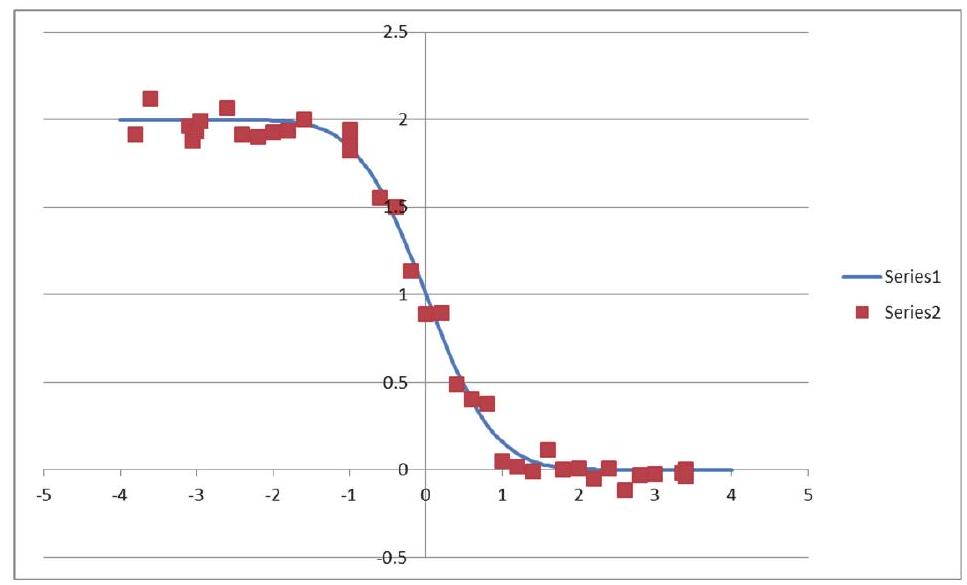
\includegraphics[max width=\textwidth]{2024_04_11_419211c3e451fc7cea07g-028(1)}
\end{center}

% (a)
(a)

\begin{center}
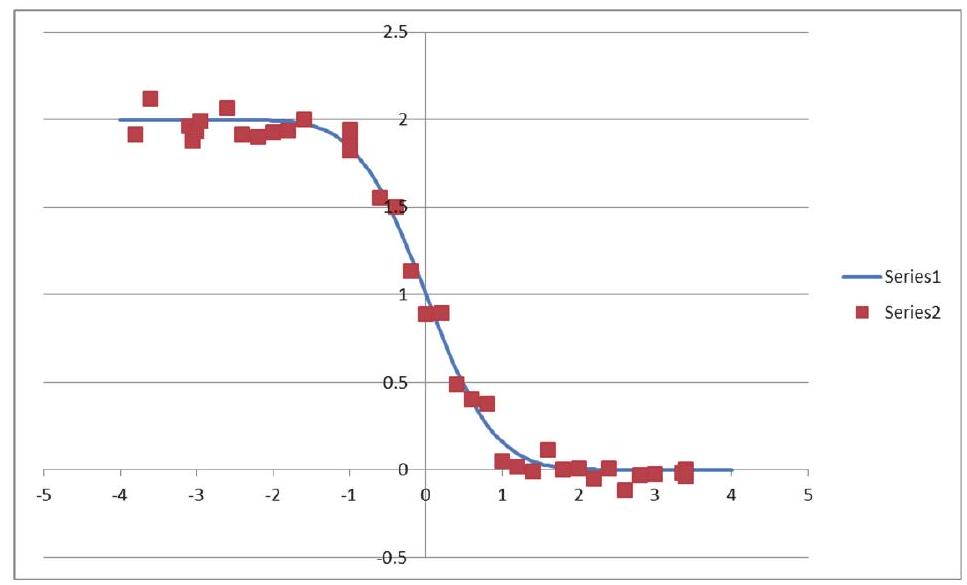
\includegraphics[max width=\textwidth]{2024_04_11_419211c3e451fc7cea07g-028(1)}
\end{center}
\begin{center}
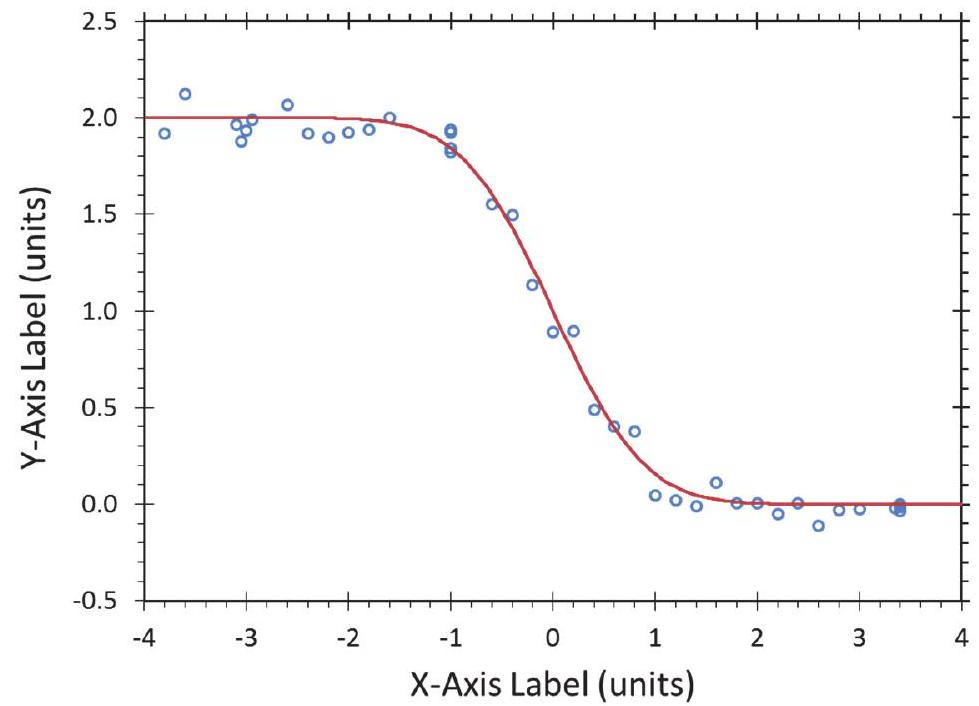
\includegraphics[max width=\textwidth]{2024_04_11_419211c3e451fc7cea07g-028}
\end{center}

% (b)
(b)

% Figure 4.1 Excel graphs of the same data: (a) default scatterplot settings, and (b) after proper formatting. Symbols show data, and the solid line shows the fitted equation.
图4.1 同一数据的Excel图表:(a) 默认散点图设置,(b) 经过适当格式化后的图表。符号表示数据,实线表示拟合方程。

% submission to a scientific journal. My example will be simple: a plot of (made-up) experimental data along with an equation that models that data. The before and after plots are shown in Fig. 4.1.
向科学期刊提交。我的例子会很简单:一张(虚构的)实验数据图以及一个模拟该数据的方程式。前后对比图示展示在图4.1中。

% Here is the sequence of steps I went through in Excel to move from the default (Fig. 4.1(a)) to the final graph (Fig. 4.1(b)). I assumed that the final graph will fit within a single column in a two-page-per-column format. For journals with other page formats, some adjustments to these directions may be required.
这是我在Excel中从默认状态(图4.1(a))转移到最终图表(图4.1(b))所经历的步骤顺序。我假设最终图表将适合在双页并排格式中的单列内。对于具有其他页面格式的期刊,可能需要对这些说明进行一些调整。

\begin{enumerate}
%   \item Set the chart area size to be $5 \mathrm{in}$. tall by $6.75 \mathrm{in}$. wide (this is $2 \times$ the final size required by most journals, but it will shrink $50 \%$ when published because most scatterplots will fit in one column). The chart area height can be adjusted as needed, if the data suggest a better shape, but the 4:3 aspect ratio used here is a good default.
\item 将图表区域大小设置为高5英寸,宽6.75英寸(这通常是大多数期刊所需最终大小的2倍,但在发布时它会缩小50%,因为大多数散点图都能适应单列的宽度)。如果数据提示更适合其他形状,图表区域的高度可以按需调整,但这里使用的4:3宽高比是一个很好的默认设置。

%   \item Set the chart font size to be 14 points (the size will be $7 \mathrm{pt}$ after shrinking the graph $50 \%$ ).
\item 将图表字体大小设置为14点(缩小图表50%后,字体大小将为7点)。

%   \item Remove the legend if not needed (try to put labels inside the graph if they fit rather than using a legend). If using a legend, see if there is room within the plot area to put it. In Fig. 4.1, using the convention of symbols for data and a line for the theoretical equation means that the legend can be embedded in the caption.
\item 如果不需要图例,请将其删除(如果标签能适合放入图表内部,则优先使用标签而不是图例)。如果使用图例,请查看绘图区域内是否有空间放置它。在图4.1中,使用符号表示数据和线条表示理论方程的惯例意味着图例可以嵌入到标题中。

%   \item Remove all gridlines.
\item 移除所有网格线。

%   \item Change the axes' line color from gray (the Excel default) to black and set it to $1 \mathrm{pt}$ thick.
\item 将坐标轴的线条颜色从灰色(Excel默认颜色)更改为黑色,并将其设置为1磅厚。

%   \item Change the major tick mark to "cross" and minor tick mark to "outside."
\item 将主要刻度标记更改为“十字”,并将次要刻度标记更改为“外侧”。

%   \item Format the chart area to have no border.
\item 设置图表区域无边框。

%   \item Format the plot area to have a solid black border (1 pt thick) and no fill.
\item 将绘图区域格式设置为具有1点厚的实心黑色边框,且无边框填充。

%   \item Set the "axis crosses" point so that the two axes meet at the lower-left corner.
\item 设置“坐标轴交叉”点,使得两条坐标轴在左下角相交。

%   \item Adjust the axes' label numbers so that they have the proper number of decimal points.
\item 调整坐标轴标签的数字,使它们具有正确的小数点位数。

%   \item If necessary, adjust the axes' min and max values (Excel defaults are often poor). Remember that the goal is to use up almost all of the graph space with data, but try to keep the data points from overlapping onto the solid border surrounding the plot area.
\item 如果需要,调整坐标轴的最小和最大值(Excel的默认值通常不好)。请记住,我们的目标是让数据几乎占据整个图表空间,但尽量保持数据点不要与围绕绘图区域的实线边界重叠。

%   \item Add axis titles, set to $18 \mathrm{pt}$ (less if titles are too long), no bold, and use a rotated vertical title.
\item 添加坐标轴标题,设置为18磅(如果标题太长可以更小),不要加粗,并使用旋转的垂直标题。

%   \item Format the "data series" to have the preferred color and symbol or line type/style for maximum readability and differentiation between data series. I typically use a weight of $1.5 \mathrm{pt}$ for my lines, and my preferred symbol is the open circle when more than one thing is being plotted at a time or when data points overlap.
\item 将“数据序列”格式设置为具有最佳可读性和数据序列间区分度的首选颜色、符号或线条类型/样式。我通常将线条权重设置为1.5磅,当一次要绘制多个事物或数据点重叠时,我偏爱的符号是开放圆圈。

%   \item If using line segments to connect data points, never turn on the "smoothed line" feature.
\item 如果使用线段连接数据点,永远不要开启“平滑线”功能。

%   \item Make sure that there is no title.
\item 确保没有标题。

%   \item Add a baseline in the graph if doing so is helpful for interpreting the data, but do not include a $y=0$ line by default.
\item 如果在图中添加基线有助于解释数据,那么就添加一个基线,但默认情况下不要包括 $y=0$ 的线条。

%   \item Preferred: put tick marks on the right and top of the plot area bounding box (this is tricky to do in Excel; use a "secondary axis").
\item 首选:在绘图区域边界框的右侧和顶部放置勾选标记(在Excel中这样做比较棘手,需要使用“次坐标轴”)。

\end{enumerate}

% That is a lot of steps, but every step left out produces a less adequate graph. Note that some of these steps can be described as aesthetic, though making a graph more pleasing to the eye is generally synonymous with making it more readable. For example, the open-circle data symbols enable one to see behind the symbol to the line and to other data points. In the original graph with the solid square symbols, can you tell how many data points are at $x=-1$ and $x=3.4$ ? When using more than one symbol, be sure to consider the symbols' size and shape for maximum visibility when there is overlap.
那是很多步骤,但每省略一步都会导致图表不够完善。请注意,其中一些步骤可以被认为是出于美观考虑,尽管使图表看起来更悦目通常与提高可读性是同义的。例如,开放圆圈数据符号能让人们看到符号背后的线条和其他数据点。在原始的用实心正方形符号的图表中,你能说出$x=-1$和$x=3.4$时有多少个数据点吗?当使用多个符号时,务必考虑符号的大小和形状,以在重叠时确保最大可见性。

% \subsection*{4.5.2 Other scatterplot examples}
\subsection*{4.5.2 其他散点图示例}
% The next example (Fig. 4.2) shows how labels can sometimes be fit into the graph to avoid the need to refer back and forth to a legend.
下一个例子(图4.2)展示了如何有时将标签放入图表中,以避免反复参照图例。

% A regular problem I encounter is a graph with data that fails to use up the space in the plot area. In Fig. 4.3, the authors wish to show the stability of their laser, so they stretch the $y$-axis range to be ten times the data range. As result, we cannot see the variation in the data. So why bother showing the graph? A similar
我经常遇到的一个问题是有数据的图表未能充分利用绘图区域的空间。在图4.3中,作者希望展示他们激光的稳定性,因此他们将$y$轴的范围放大到数据范围的十倍。结果,我们无法看到数据中的变化。那么,展示这样的图表又有何意义呢?类似的情况是

\begin{center}
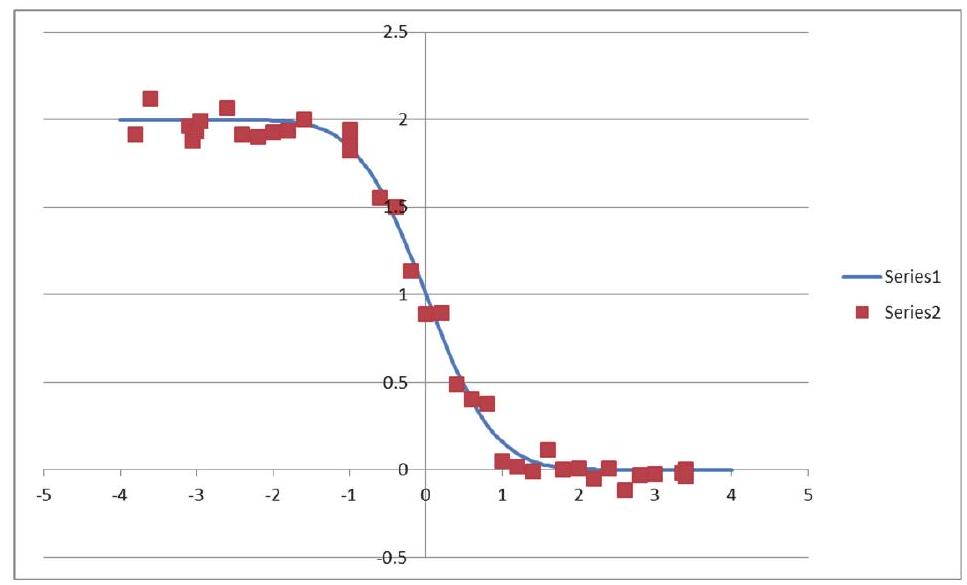
\includegraphics[max width=\textwidth]{2024_04_11_419211c3e451fc7cea07g-028(1)}
\end{center}
\begin{center}
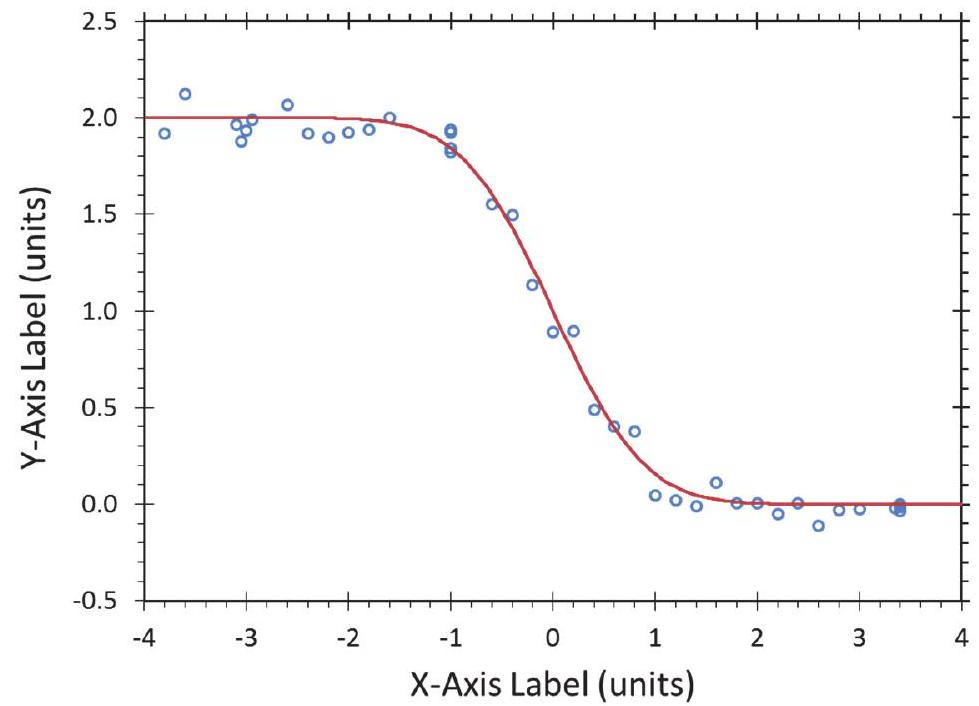
\includegraphics[max width=\textwidth]{2024_04_11_419211c3e451fc7cea07g-028}
\end{center}
\begin{center}
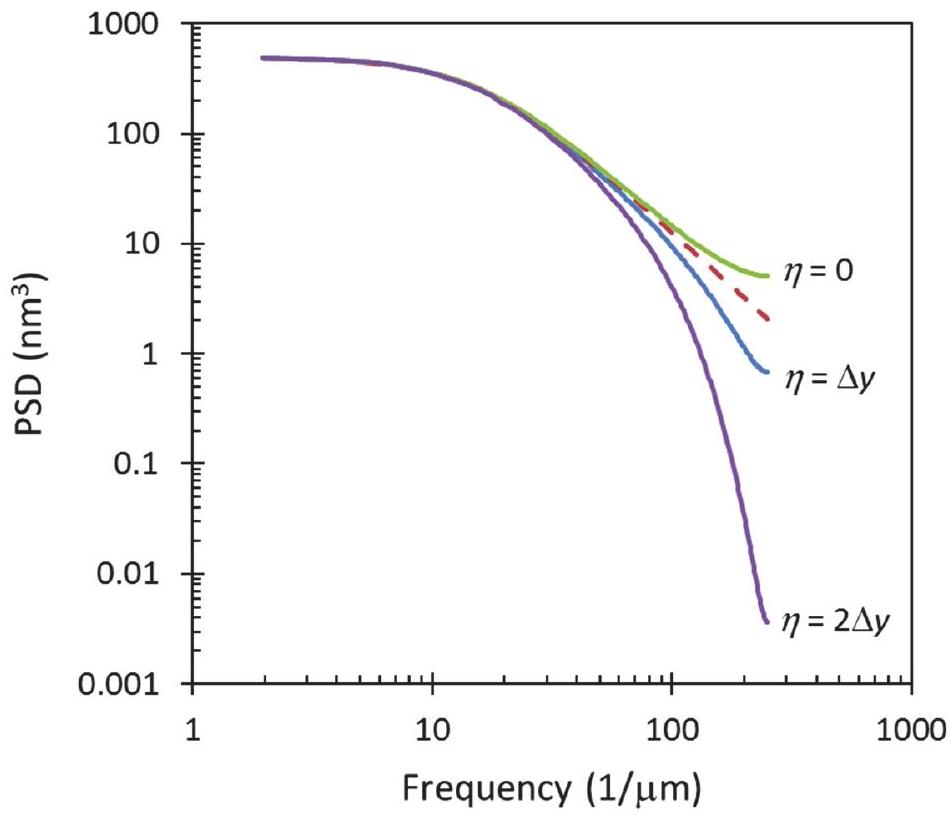
\includegraphics[max width=\textwidth]{2024_04_11_419211c3e451fc7cea07g-030}
\end{center}

% Figure 4.2 Labels within the graph avoid the need for a legend. The color used here improves readability online but is not needed for comprehension when printed in black and white. The dotted line is explained as being the reference curve in the figure caption of the original. ${ }^{16}$
图4.2 图内的标签避免了需要图例。这里使用的颜色提高了在线阅读性,但在黑白打印时并不需要理解内容。虚线在原图的图注中被解释为参考曲线。${ }^{16}$

\begin{center}
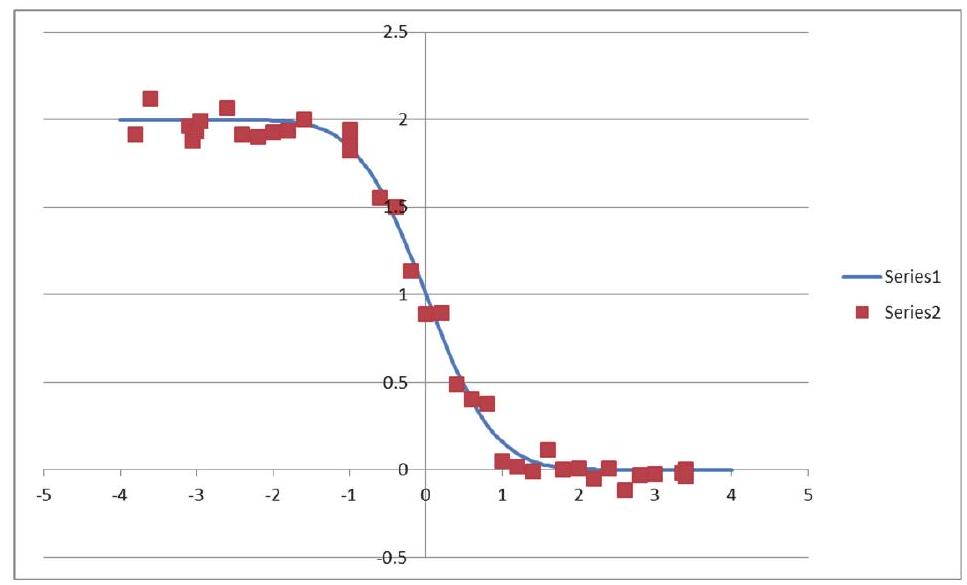
\includegraphics[max width=\textwidth]{2024_04_11_419211c3e451fc7cea07g-028(1)}
\end{center}
\begin{center}
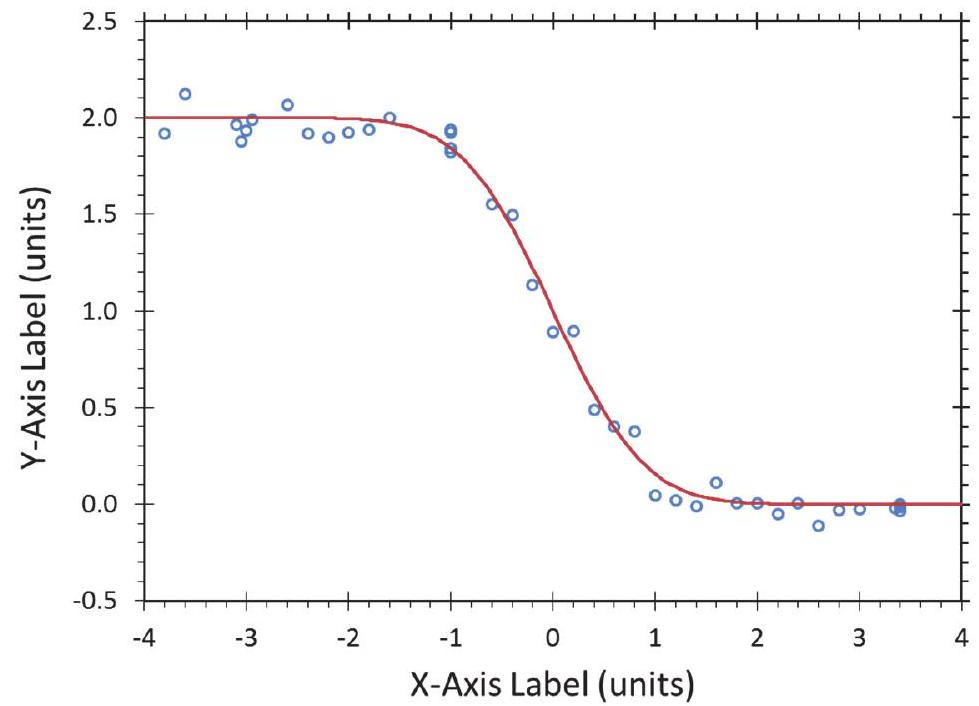
\includegraphics[max width=\textwidth]{2024_04_11_419211c3e451fc7cea07g-028}
\end{center}
\begin{center}
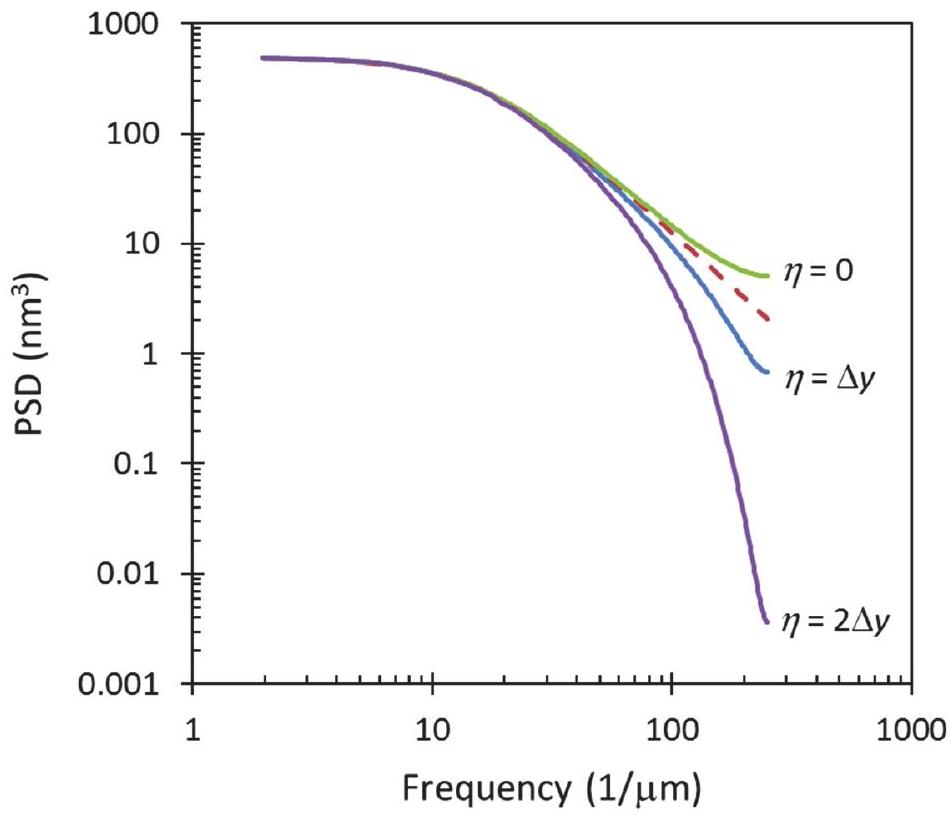
\includegraphics[max width=\textwidth]{2024_04_11_419211c3e451fc7cea07g-030}
\end{center}
\begin{center}
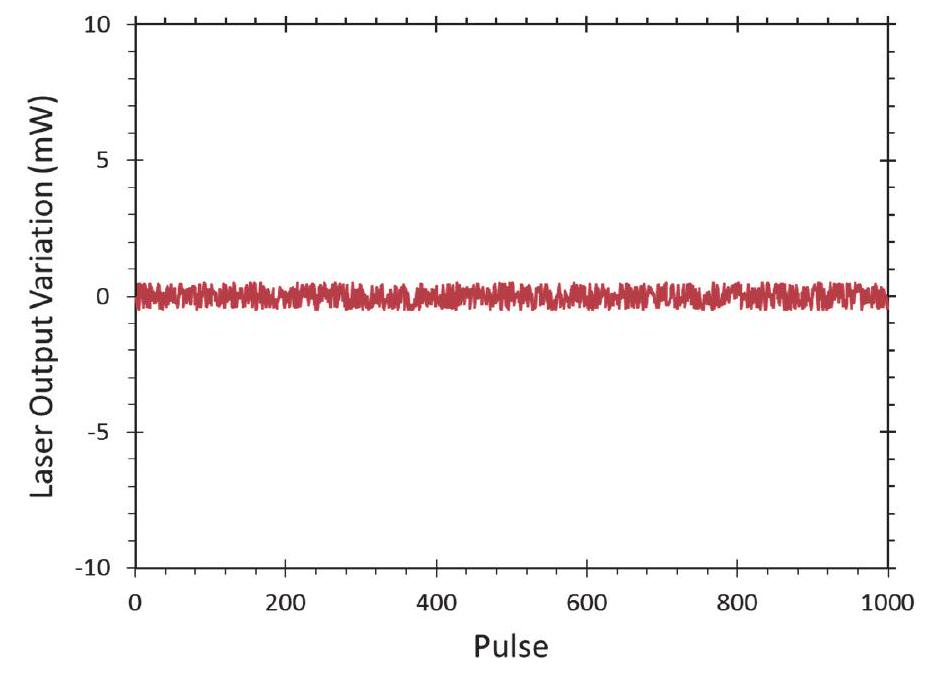
\includegraphics[max width=\textwidth]{2024_04_11_419211c3e451fc7cea07g-031}
\end{center}

% Figure 4.3 A wasted graph. The $y$ axis is chosen to give the impression that the there is little variation in the output, but if we cannot see any variation in the data, why show the graph?
图4.3 一个浪费的图表。选择 $y$ 轴以给人输出变化很小的印象,但如果我们看不到数据中的任何变化,为什么还要展示这个图表呢?

% effect can be obtained by including zero on the $y$-axis scale even though no data are near zero (imagine a plot of Earth's global surface temperature in Kelvin over time, then starting the $y$ axis at zero-global warming would disappear). This is an example of advocating rather than informing, i.e., using graphs to hide rather than reveal the truth. If there is nothing in the data worth seeing, the graph should be replaced with simple statistics: mean, standard deviation, $\min / \max$ of the output, and maybe a statement that a linear regression gave a slope that was not statistically different from zero. If there is something worth seeing in the data, then adjust the $y$-axis scale so that it can be seen.
即使没有数据接近零,通过在y轴刻度上包含零也可以获得效果(想象一下,绘制地球全球表面温度随时间变化的曲线图,如果从零开始y轴,那么全球变暖就会消失)。这是倡导而非告知的一个例子,即使用图表隐藏而非揭示真相。如果数据中没有值得注意的内容,应该用简单的统计信息替换图表:平均值、标准差、输出的最小/最大值,也许还可以说明线性回归的斜率在统计上与零没有差异。如果数据中有值得注意的内容,那么调整y轴的刻度以便能够看到。

% There are other ways to mislead with an $x-y$ scatterplot, some not as subtle as the previous example. Unitless axes are a favorite of those who, at a minimum, do not wish to reveal the whole truth. An axis with ambiguous labeling should never be allowed. Using "arbitrary units" for a $y$-axis is a bit trickier because there are some cases where such a label is appropriate (a relative measure, based on a local uncalibrated standard that can be used to compare similar measurements). A common example is the relative intensity used in spectral analysis. Arbitrary units are never preferred but sometimes necessary. Arbitrary units should never be used to hide known units that the author does not want to reveal. Additionally, arbitrary units have an arbitrary scale but not an arbitrary zero point. Thus, when arbitrary units are used the graph must mark the zero point on the scale. One solution is to use a relative scale rather than arbitrary units, with the original clearly defined.
还有其他方法可以用$x-y$散点图误导,有些方法不如前面的例子那么微妙。无单位的坐标轴是那些至少不想揭示全部真相的人的最爱。带有模糊标记的坐标轴绝不应该被允许。在$y$轴上使用“任意单位”要更为狡猾一些,因为有些情况下这样的标签是恰当的(基于局部未校准的标准,用于比较相似测量的相对度量)。一个常见的例子是在光谱分析中使用的相对强度。任意单位从不首选,但有时是必要的。任意单位绝不应该用来隐藏作者不想透露的已知单位。此外,任意单位有任意的刻度,但没有任意的零点。因此,当使用任意单位时,图表必须在刻度上标记零点。一个解决方案是使用相对刻度而不是任意单位,并清楚定义原始刻度。

% One common and important application of the $x-y$ scatterplot compares different graphs (thus adding a third variable, sometimes more). Figure 4.4 shows a $2 \times 3$ array of graph multiples, matching the $x$-axis and $y$-axis scales to allow easy comparison. With small multiples, many more graphs can be compared.
$x-y$散点图的一种常见且重要的应用是比较不同的图表(从而引入第三个变量,有时甚至更多)。图4.4展示了一个$2 \times 3$的图表组合阵列,使得$x$轴和$y$轴的刻度一致,以便于进行比较。使用小倍数图表,可以比较更多的图表。

\begin{center}
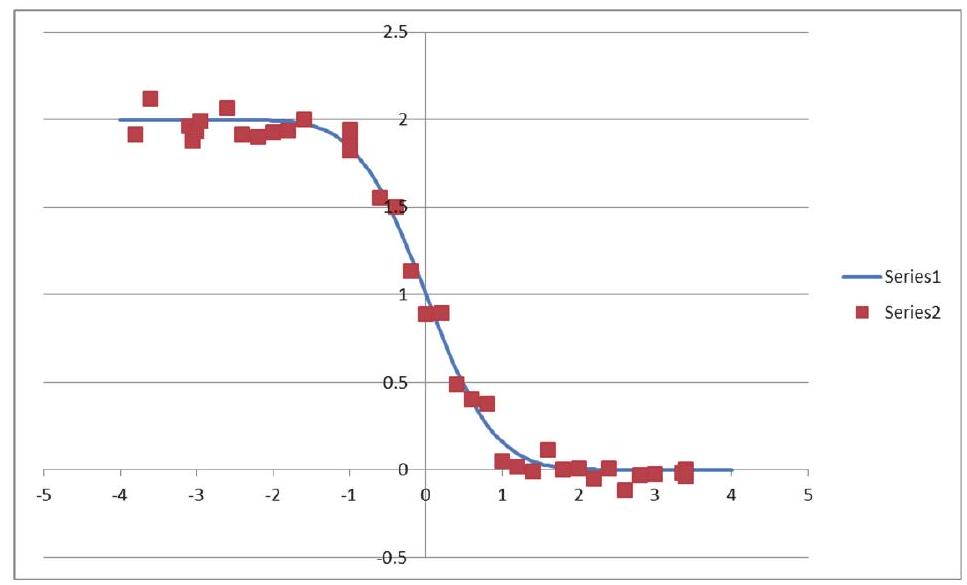
\includegraphics[max width=\textwidth]{2024_04_11_419211c3e451fc7cea07g-028(1)}
\end{center}
\begin{center}
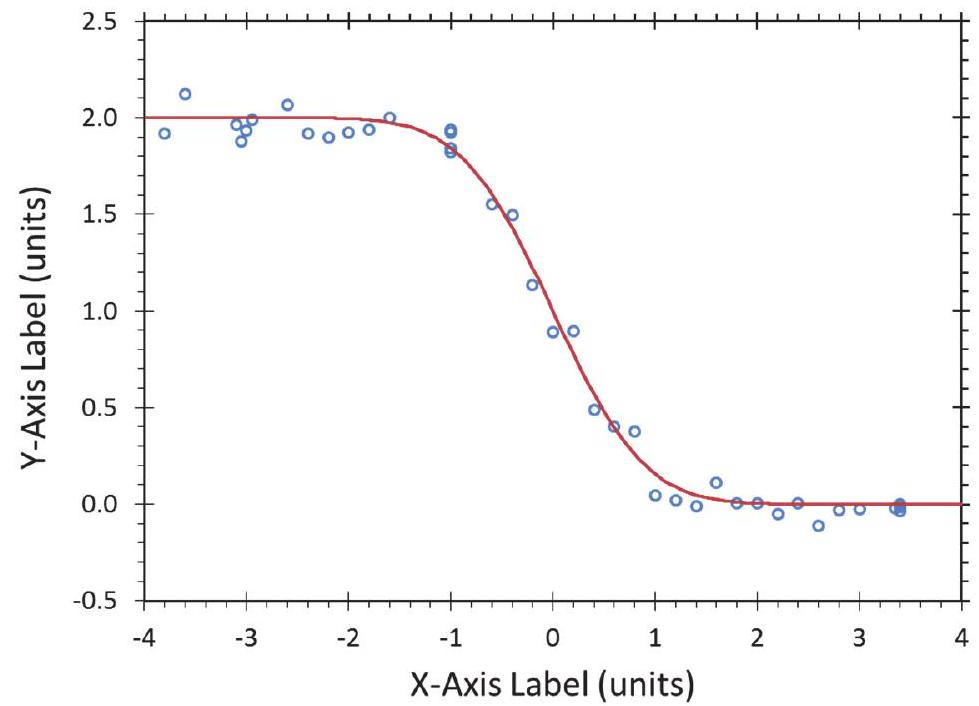
\includegraphics[max width=\textwidth]{2024_04_11_419211c3e451fc7cea07g-028}
\end{center}
\begin{center}
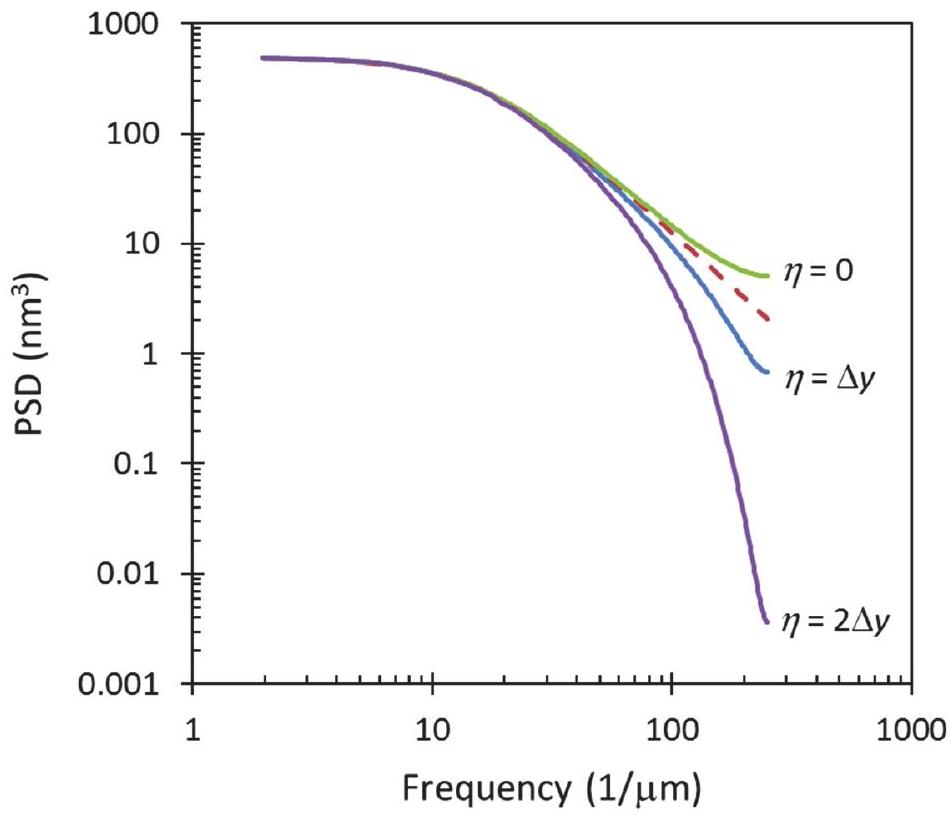
\includegraphics[max width=\textwidth]{2024_04_11_419211c3e451fc7cea07g-030}
\end{center}
\begin{center}
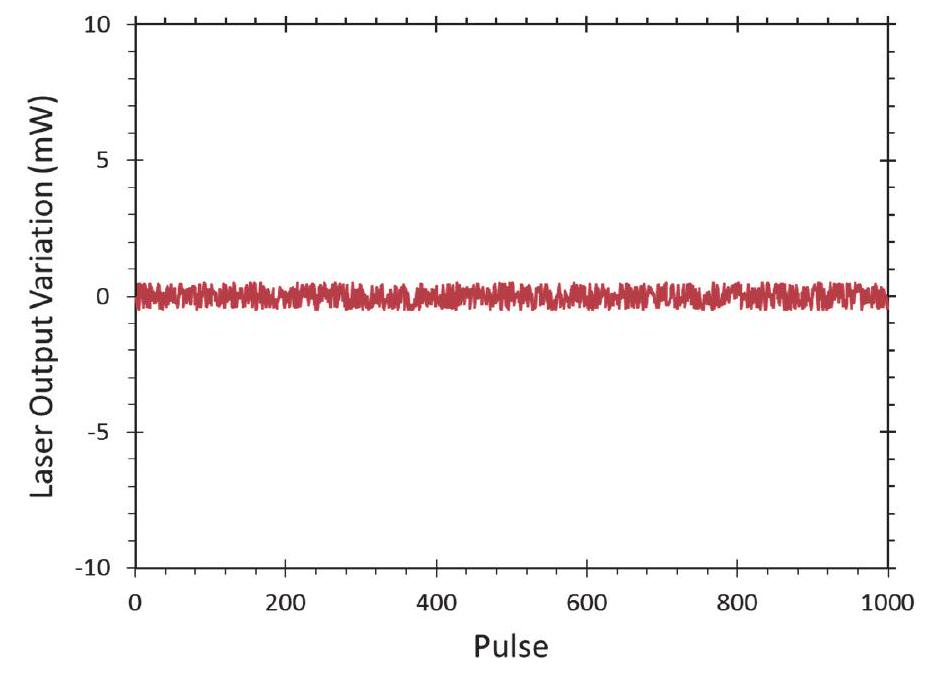
\includegraphics[max width=\textwidth]{2024_04_11_419211c3e451fc7cea07g-031}
\end{center}
\begin{center}
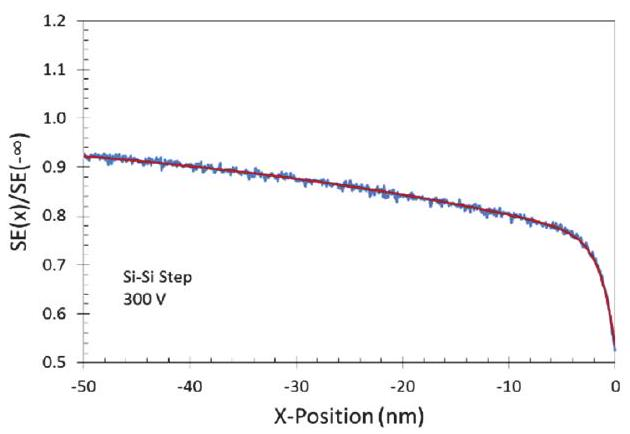
\includegraphics[max width=\textwidth]{2024_04_11_419211c3e451fc7cea07g-032(1)}
\end{center}

% (a)
(a)

\begin{center}
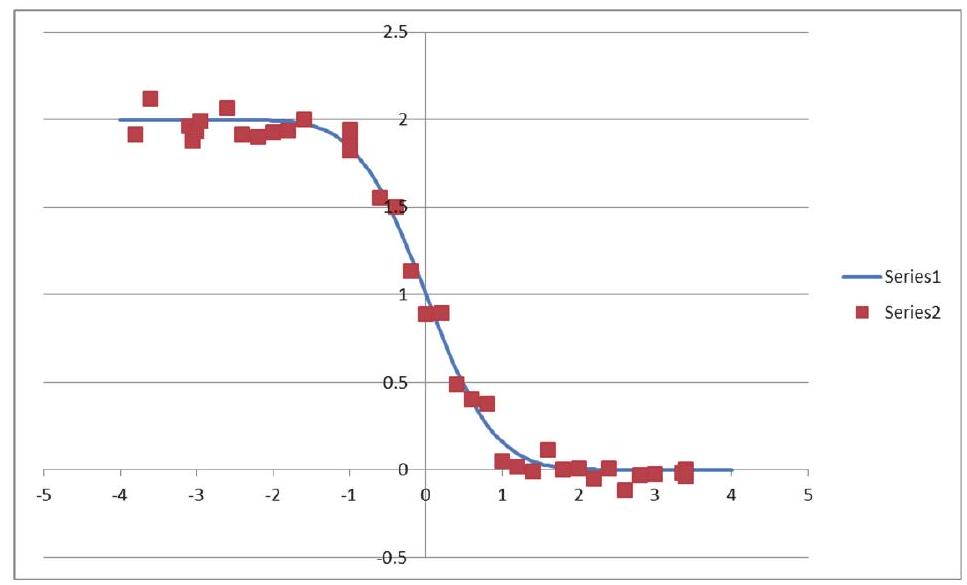
\includegraphics[max width=\textwidth]{2024_04_11_419211c3e451fc7cea07g-028(1)}
\end{center}
\begin{center}
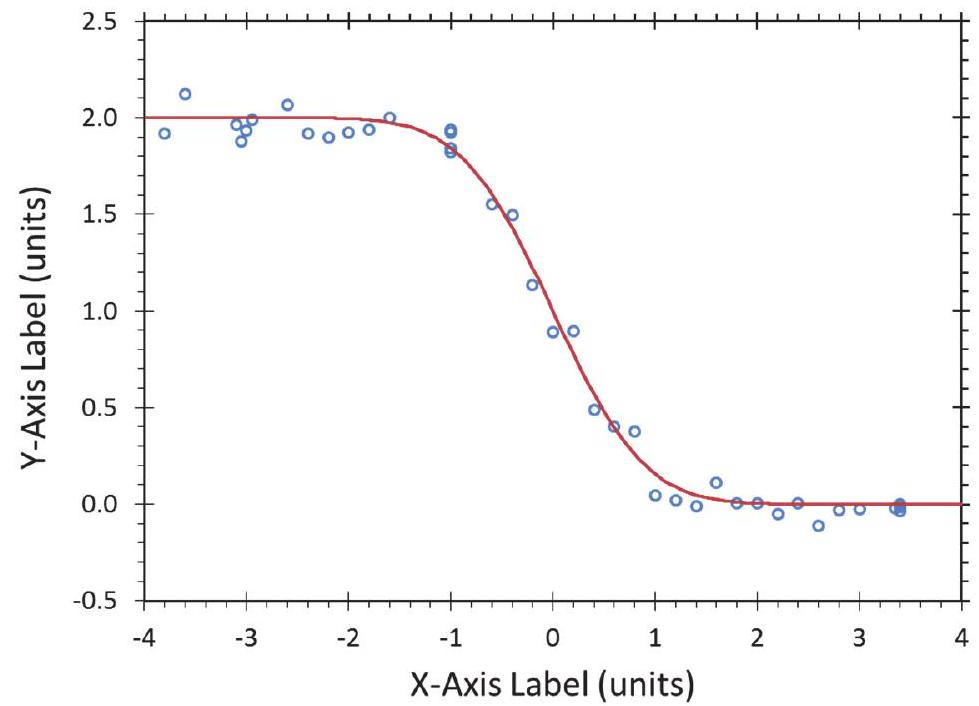
\includegraphics[max width=\textwidth]{2024_04_11_419211c3e451fc7cea07g-028}
\end{center}
\begin{center}
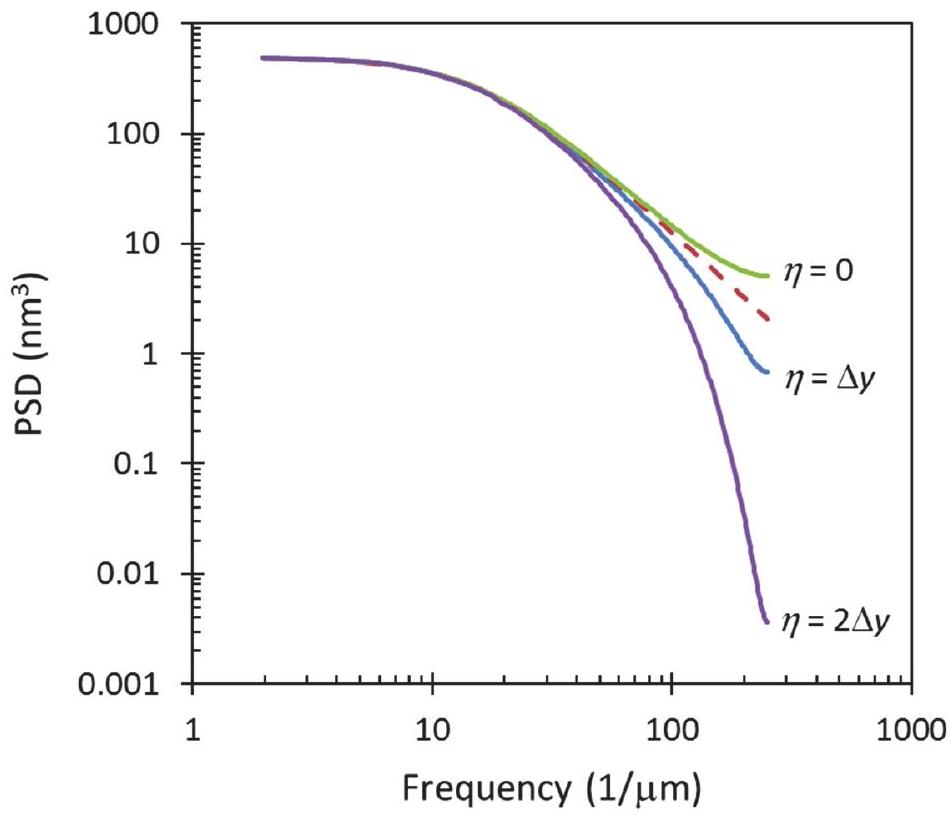
\includegraphics[max width=\textwidth]{2024_04_11_419211c3e451fc7cea07g-030}
\end{center}
\begin{center}
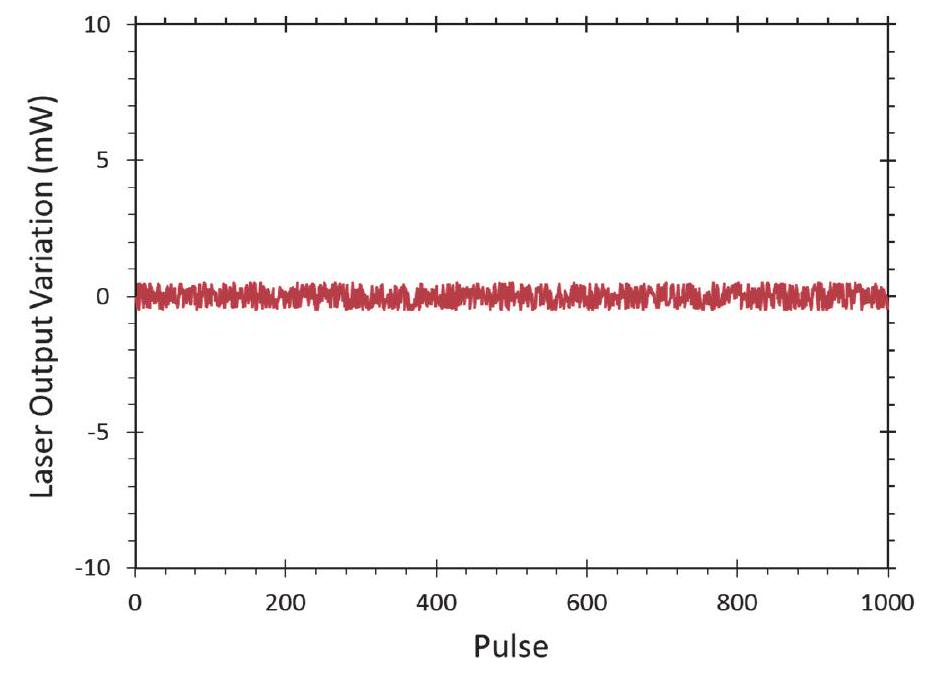
\includegraphics[max width=\textwidth]{2024_04_11_419211c3e451fc7cea07g-031}
\end{center}
\begin{center}
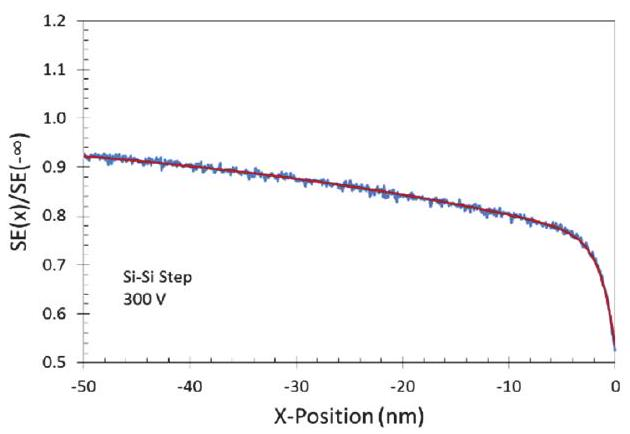
\includegraphics[max width=\textwidth]{2024_04_11_419211c3e451fc7cea07g-032(1)}
\end{center}
\begin{center}
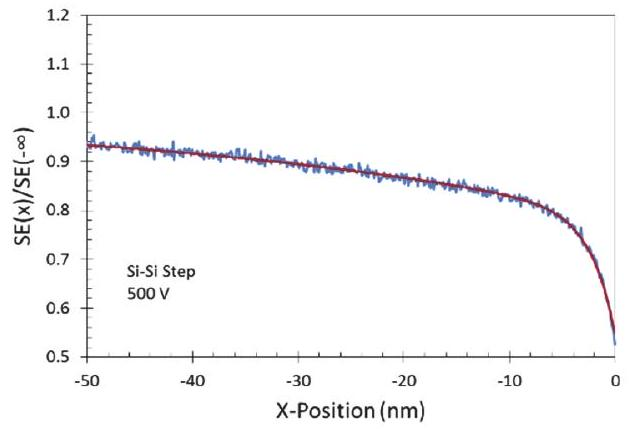
\includegraphics[max width=\textwidth]{2024_04_11_419211c3e451fc7cea07g-032(3)}
\end{center}

% (c)
(c)(版权标志)

中文通常不直接翻译这个符号,而是保留原文。(c) 表示版权所有。如果需要在中文语境中解释它的含义,可以表述为:

版权所有 ©

这里的 © 符号就是 (c) 的图形表示。

\begin{center}
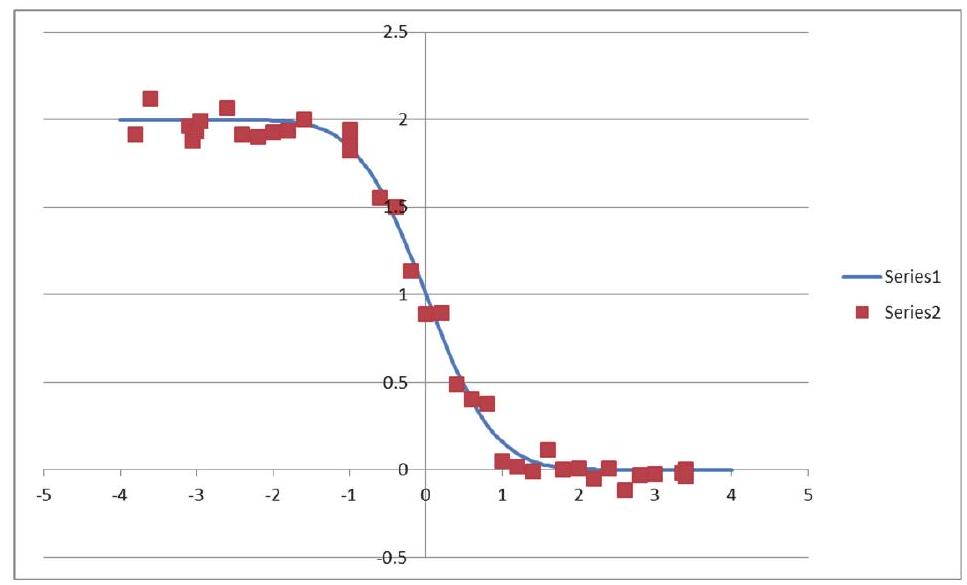
\includegraphics[max width=\textwidth]{2024_04_11_419211c3e451fc7cea07g-028(1)}
\end{center}
\begin{center}
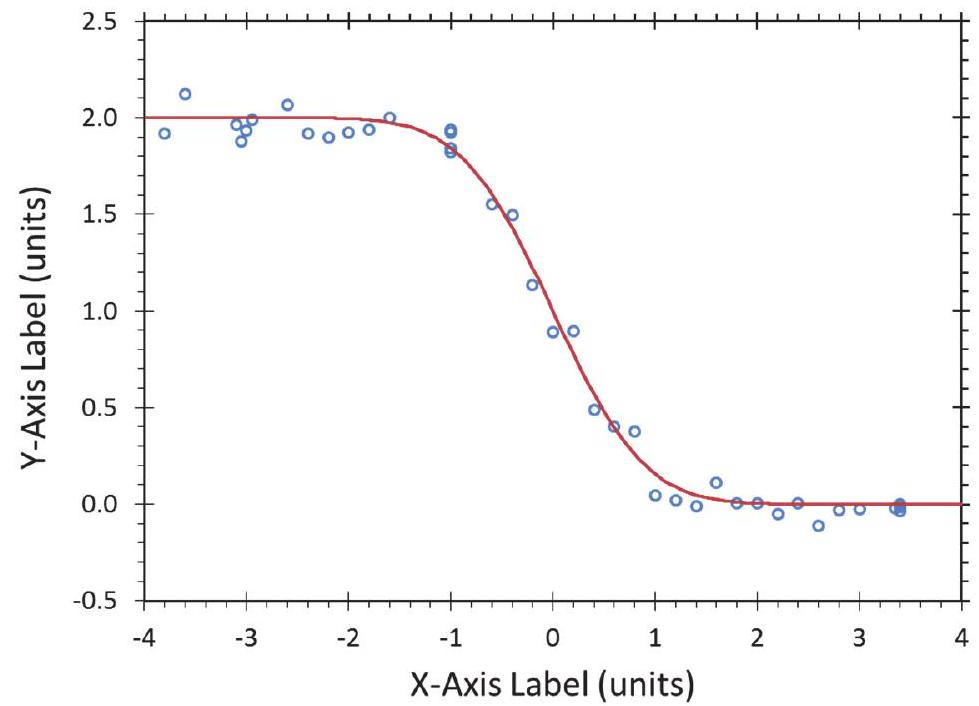
\includegraphics[max width=\textwidth]{2024_04_11_419211c3e451fc7cea07g-028}
\end{center}
\begin{center}
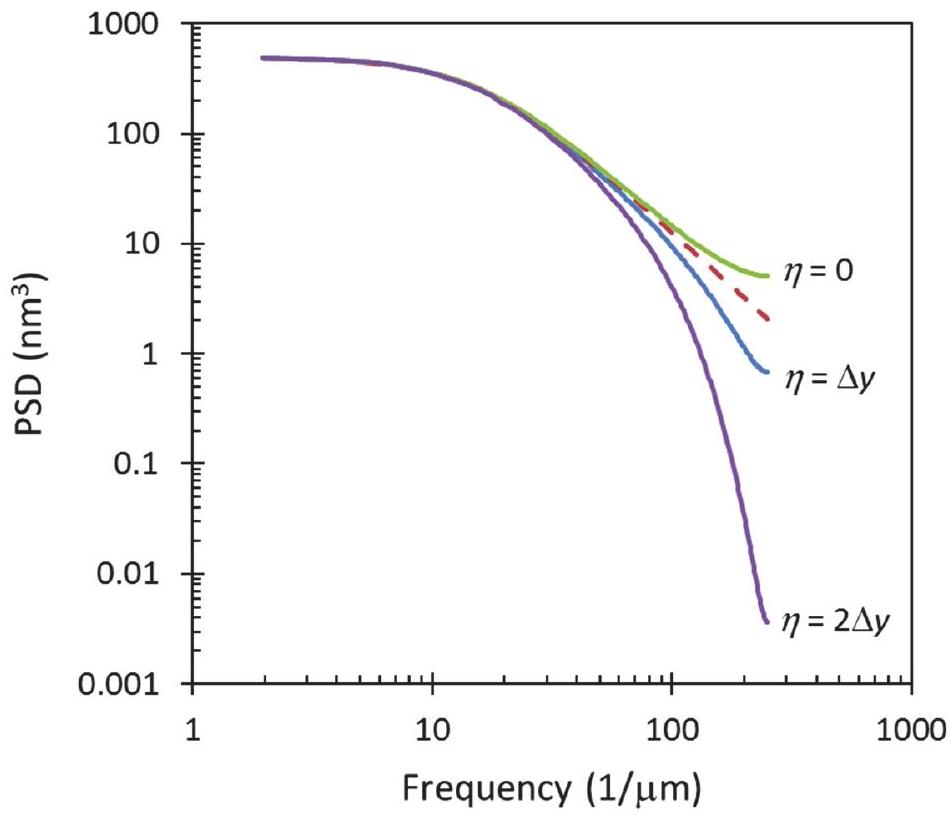
\includegraphics[max width=\textwidth]{2024_04_11_419211c3e451fc7cea07g-030}
\end{center}
\begin{center}
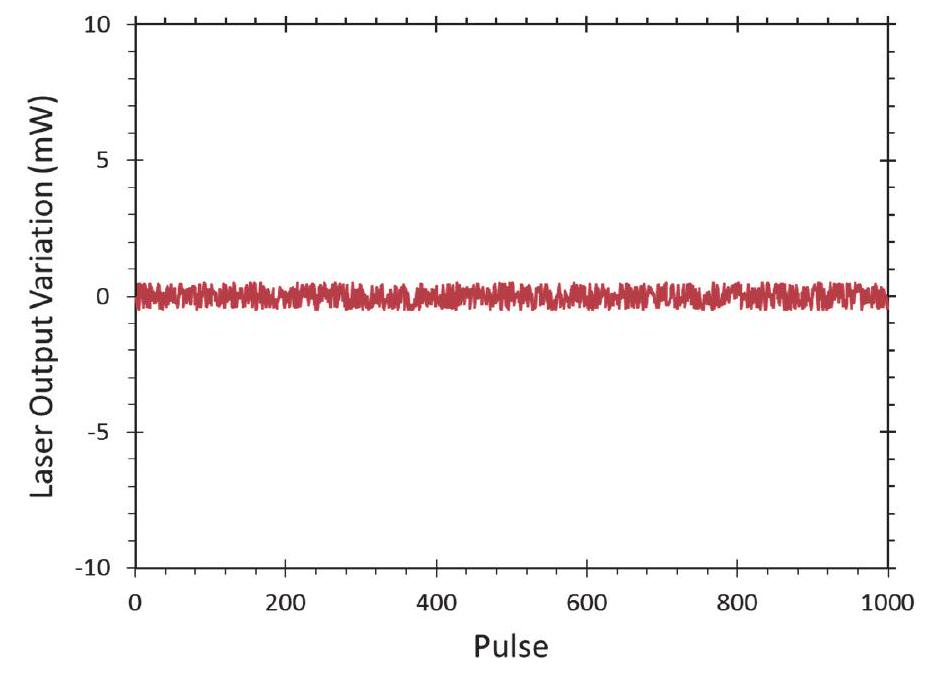
\includegraphics[max width=\textwidth]{2024_04_11_419211c3e451fc7cea07g-031}
\end{center}
\begin{center}
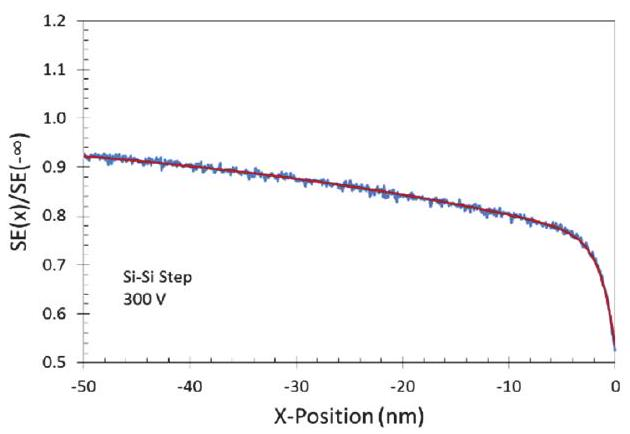
\includegraphics[max width=\textwidth]{2024_04_11_419211c3e451fc7cea07g-032(1)}
\end{center}
\begin{center}
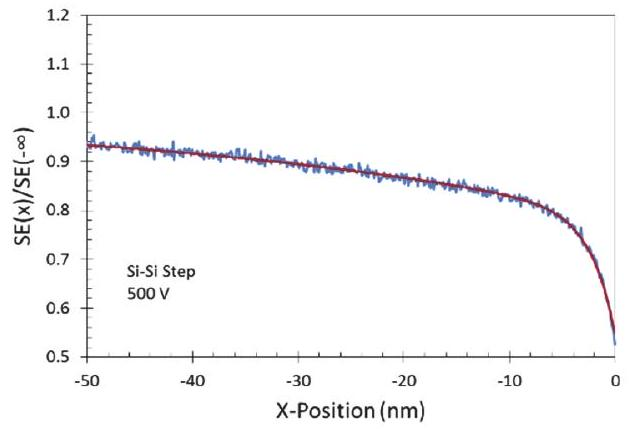
\includegraphics[max width=\textwidth]{2024_04_11_419211c3e451fc7cea07g-032(3)}
\end{center}
\begin{center}
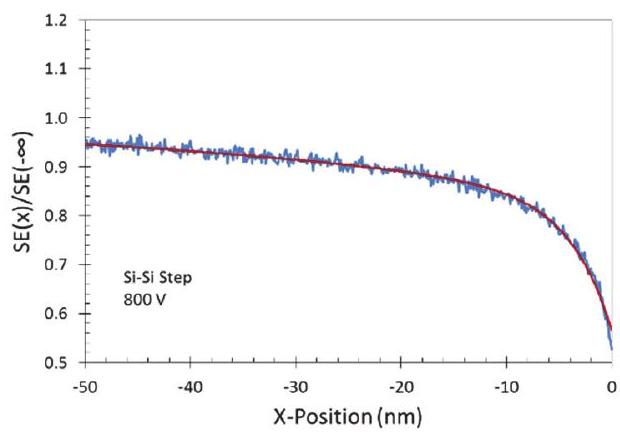
\includegraphics[max width=\textwidth]{2024_04_11_419211c3e451fc7cea07g-032(2)}
\end{center}

% (e)
(e)(这个选项似乎是未完成的或者是一个选择题中的选项。如果需要翻译整个句子或者更多的内容,请提供完整的英文句子或段落。) 

中文:(请提供完整英文内容以便翻译。)

\begin{center}
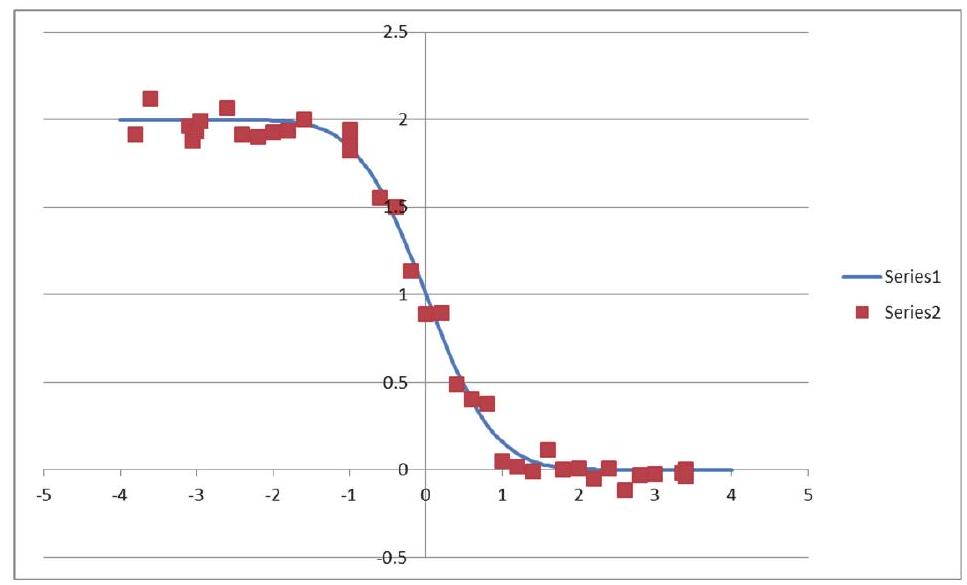
\includegraphics[max width=\textwidth]{2024_04_11_419211c3e451fc7cea07g-028(1)}
\end{center}
\begin{center}
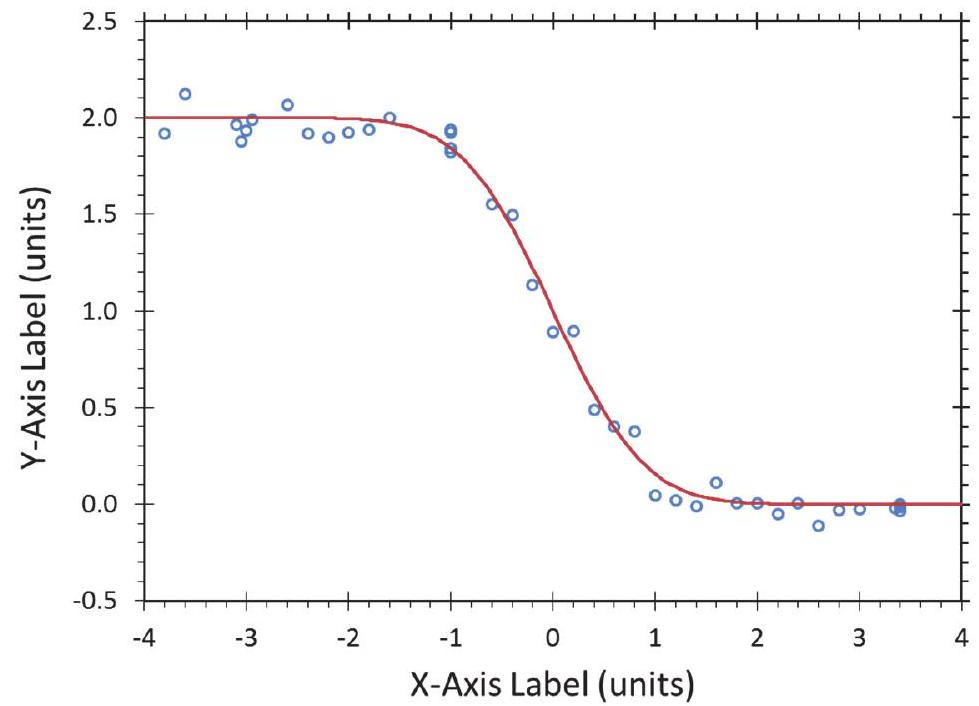
\includegraphics[max width=\textwidth]{2024_04_11_419211c3e451fc7cea07g-028}
\end{center}
\begin{center}
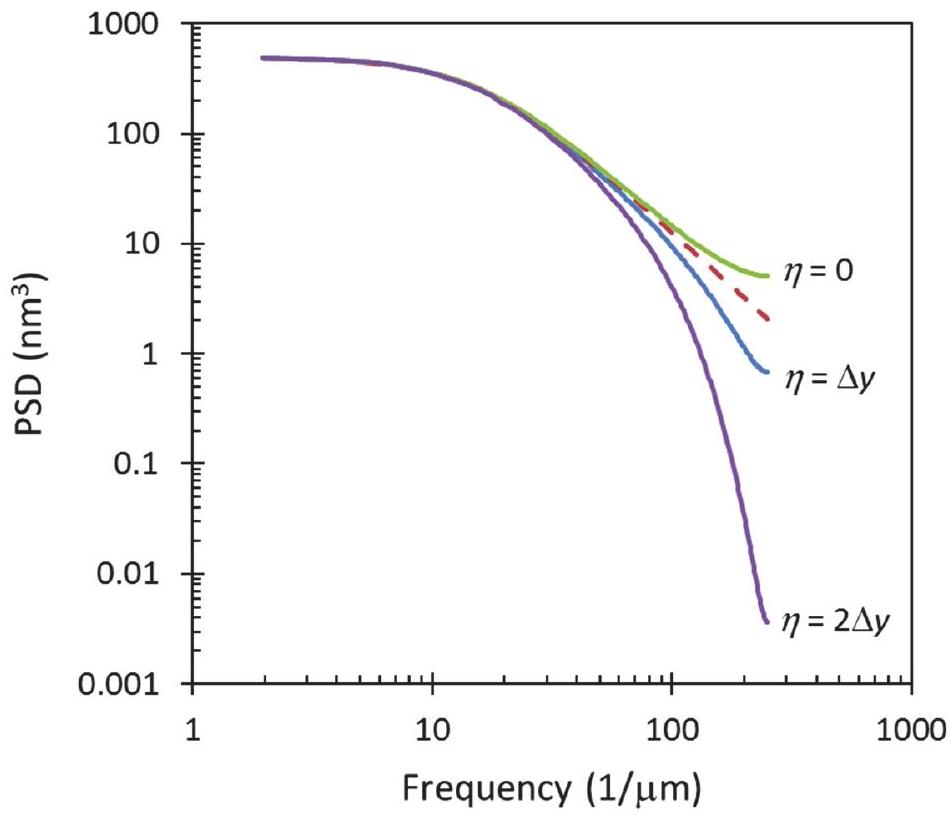
\includegraphics[max width=\textwidth]{2024_04_11_419211c3e451fc7cea07g-030}
\end{center}
\begin{center}
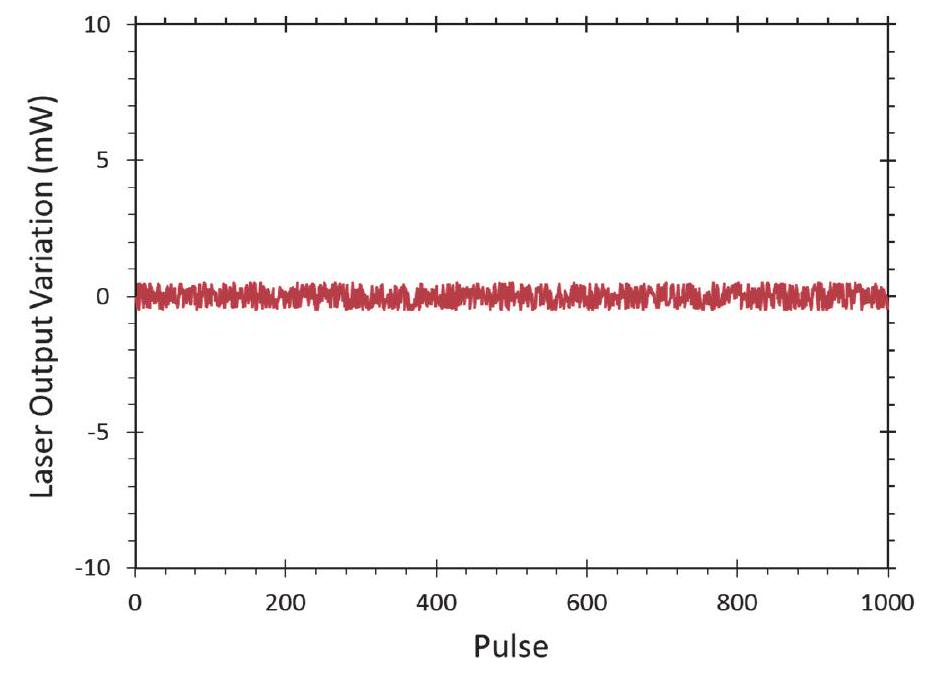
\includegraphics[max width=\textwidth]{2024_04_11_419211c3e451fc7cea07g-031}
\end{center}
\begin{center}
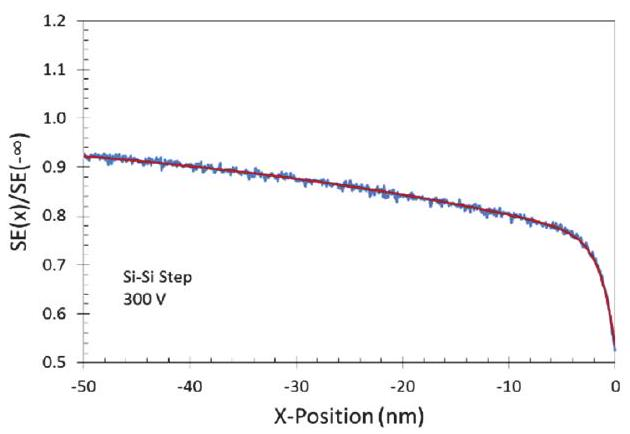
\includegraphics[max width=\textwidth]{2024_04_11_419211c3e451fc7cea07g-032(1)}
\end{center}
\begin{center}
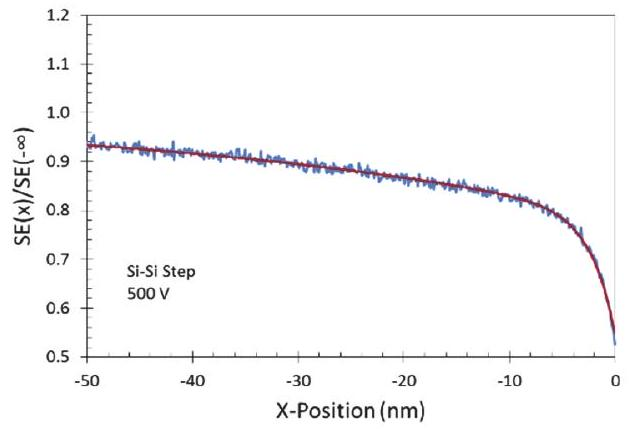
\includegraphics[max width=\textwidth]{2024_04_11_419211c3e451fc7cea07g-032(3)}
\end{center}
\begin{center}
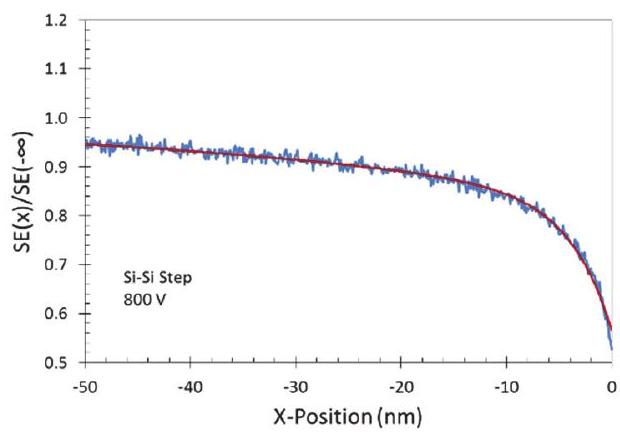
\includegraphics[max width=\textwidth]{2024_04_11_419211c3e451fc7cea07g-032(2)}
\end{center}
\begin{center}
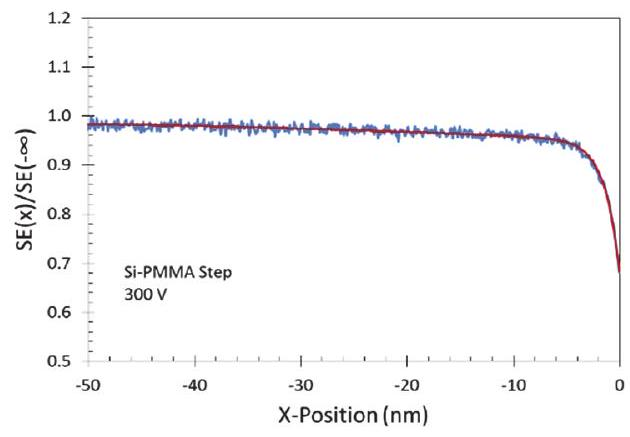
\includegraphics[max width=\textwidth]{2024_04_11_419211c3e451fc7cea07g-032(4)}
\end{center}

% (b)
(b)

\begin{center}
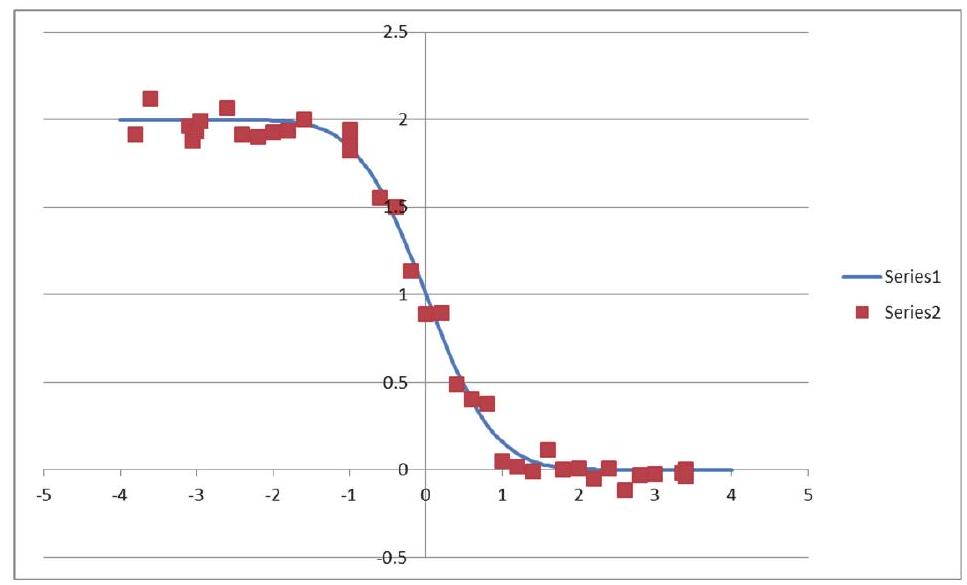
\includegraphics[max width=\textwidth]{2024_04_11_419211c3e451fc7cea07g-028(1)}
\end{center}
\begin{center}
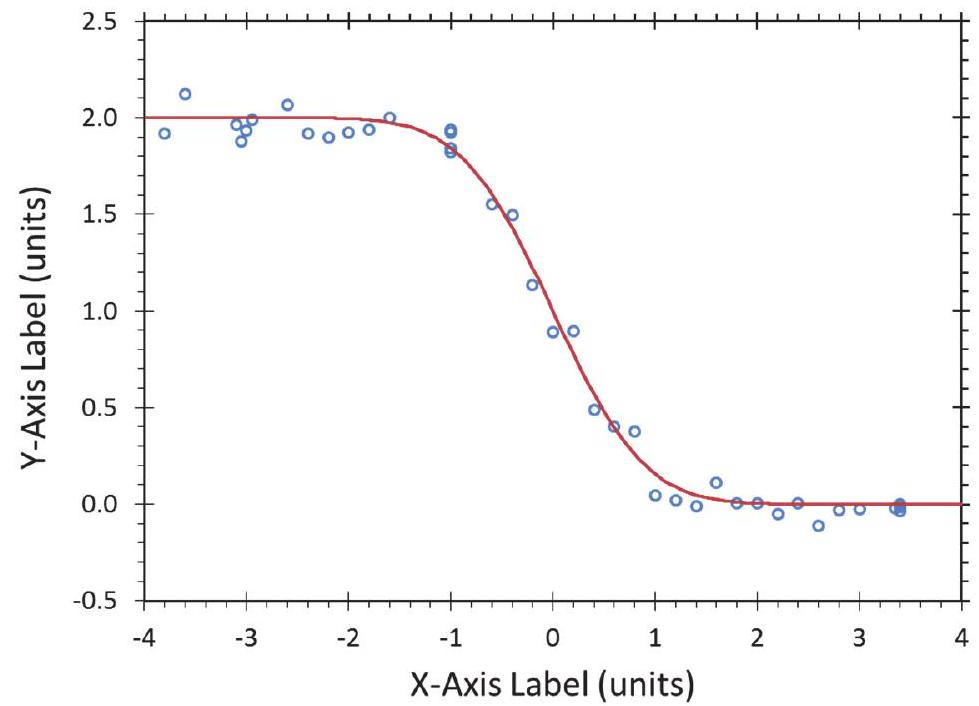
\includegraphics[max width=\textwidth]{2024_04_11_419211c3e451fc7cea07g-028}
\end{center}
\begin{center}
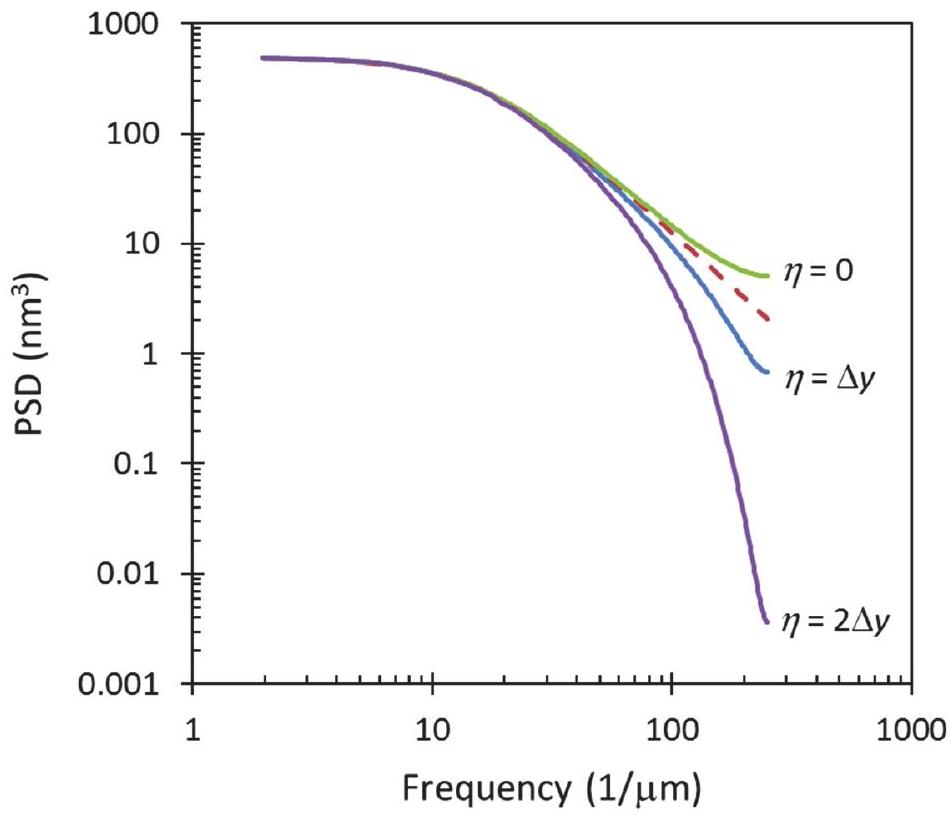
\includegraphics[max width=\textwidth]{2024_04_11_419211c3e451fc7cea07g-030}
\end{center}
\begin{center}
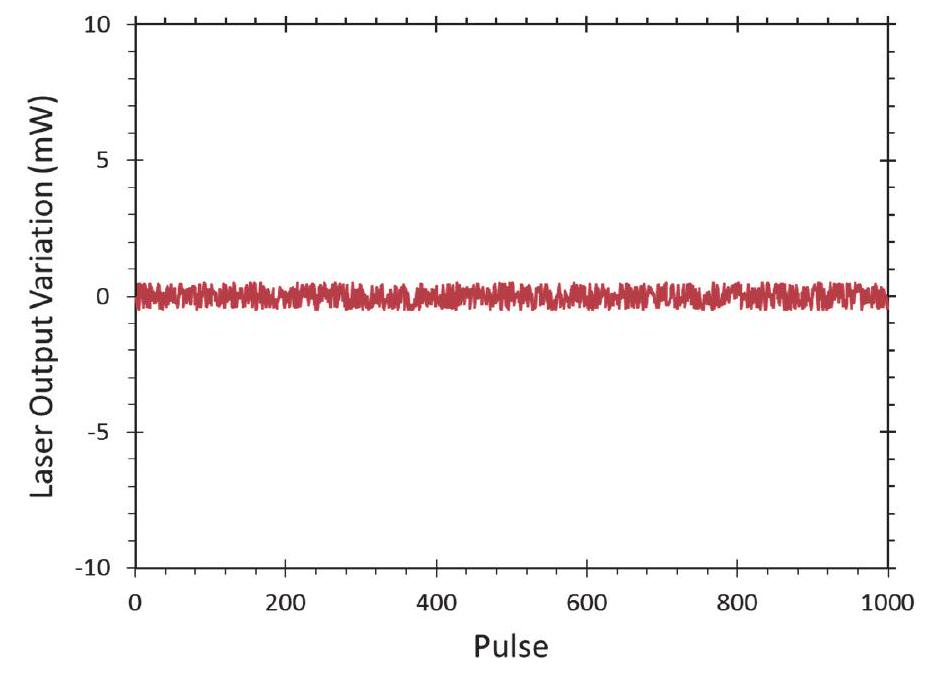
\includegraphics[max width=\textwidth]{2024_04_11_419211c3e451fc7cea07g-031}
\end{center}
\begin{center}
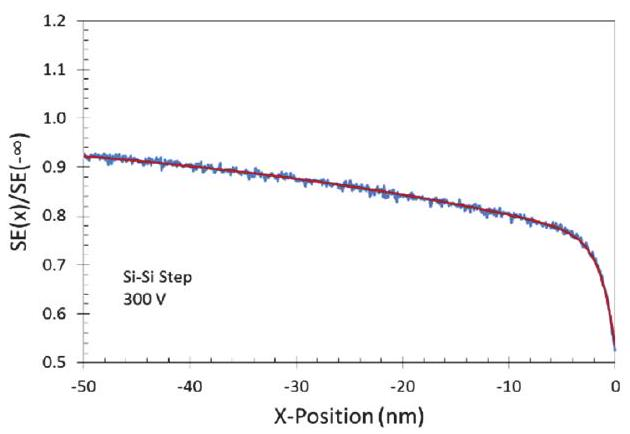
\includegraphics[max width=\textwidth]{2024_04_11_419211c3e451fc7cea07g-032(1)}
\end{center}
\begin{center}
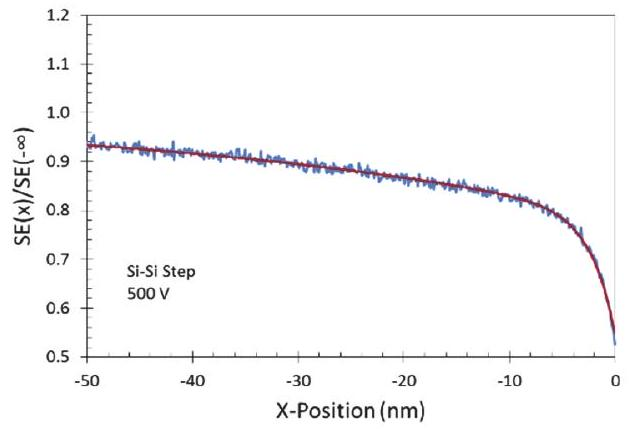
\includegraphics[max width=\textwidth]{2024_04_11_419211c3e451fc7cea07g-032(3)}
\end{center}
\begin{center}
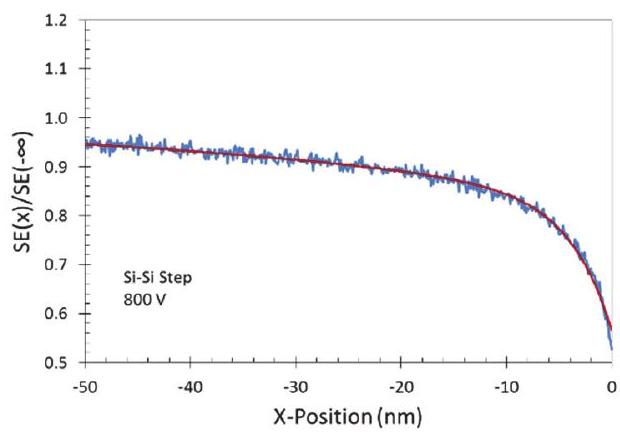
\includegraphics[max width=\textwidth]{2024_04_11_419211c3e451fc7cea07g-032(2)}
\end{center}
\begin{center}
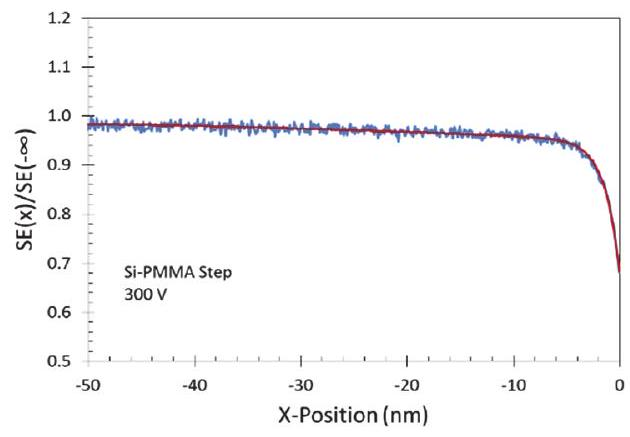
\includegraphics[max width=\textwidth]{2024_04_11_419211c3e451fc7cea07g-032(4)}
\end{center}
\begin{center}
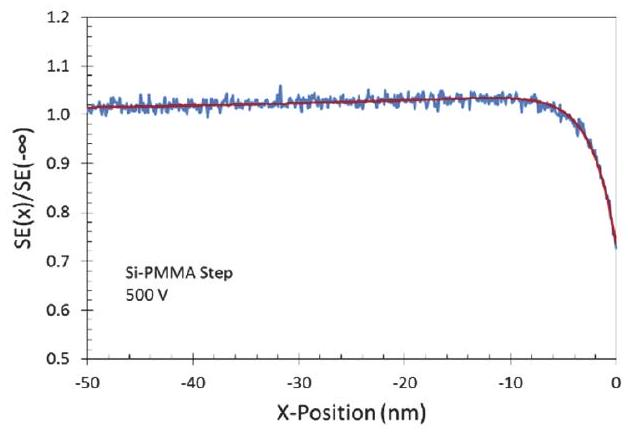
\includegraphics[max width=\textwidth]{2024_04_11_419211c3e451fc7cea07g-032(5)}
\end{center}

% (d)
(括号中的字母 d 通常不需要翻译,因为它可能表示一个选项或者是一个标记。如果需要翻译成中文,它可能会被忽略,或者根据上下文翻译为:

中文:(d) 

如果需要在选择题等场景中使用。

\begin{center}
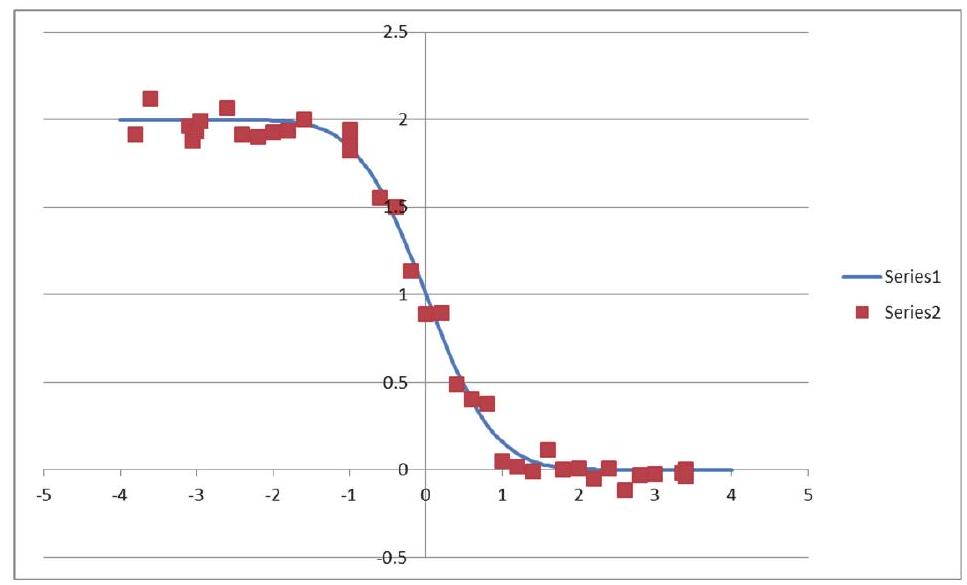
\includegraphics[max width=\textwidth]{2024_04_11_419211c3e451fc7cea07g-028(1)}
\end{center}
\begin{center}
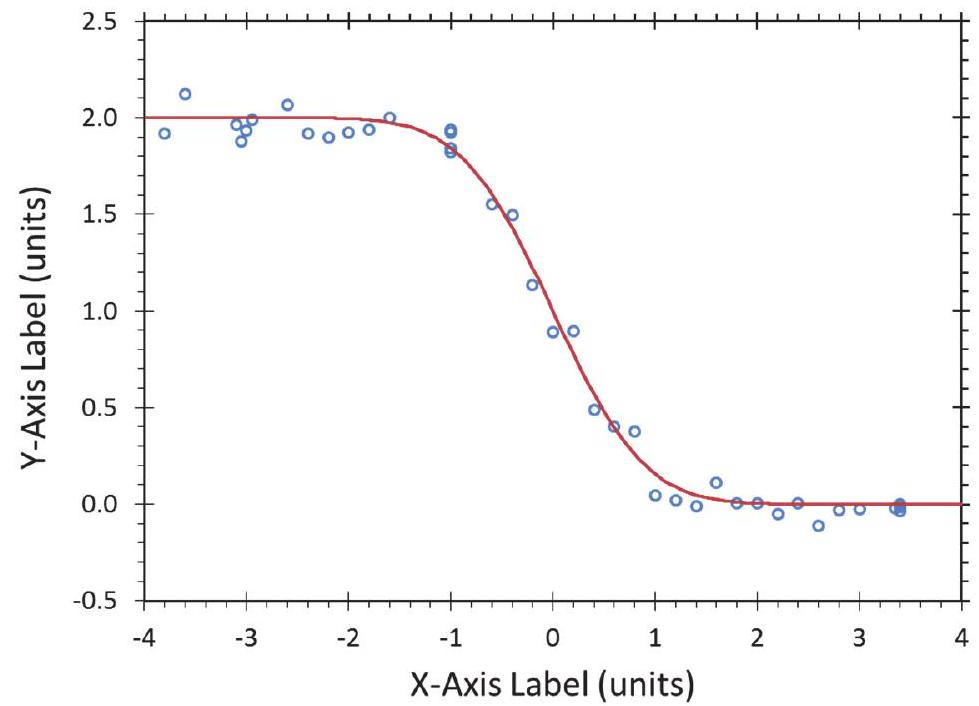
\includegraphics[max width=\textwidth]{2024_04_11_419211c3e451fc7cea07g-028}
\end{center}
\begin{center}
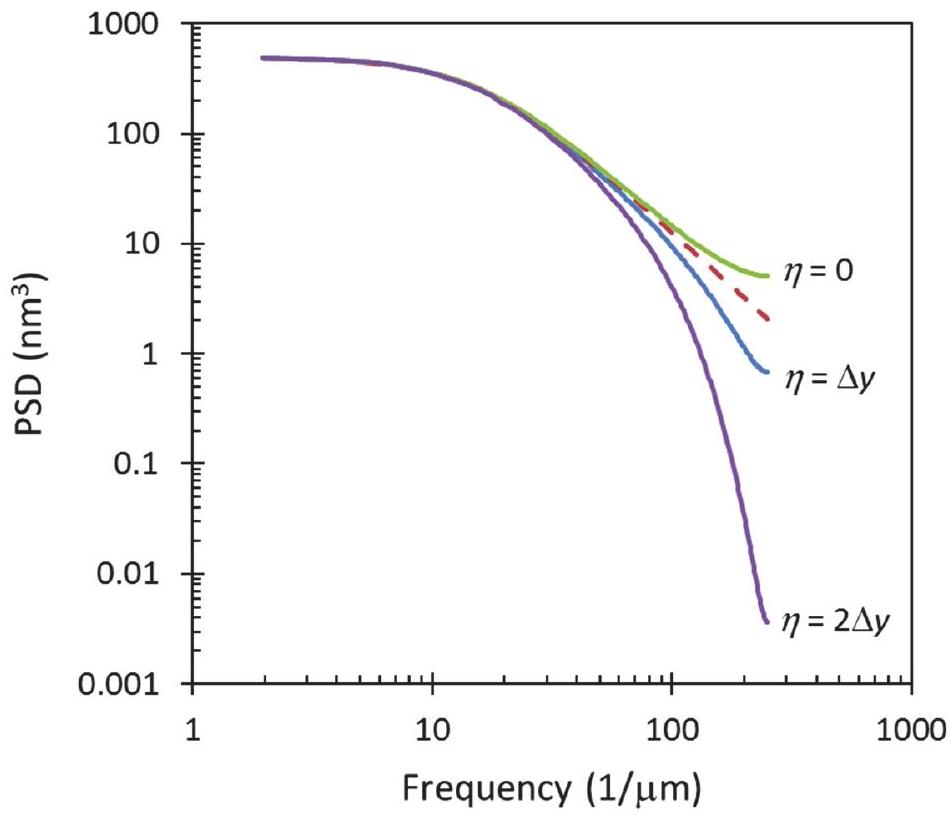
\includegraphics[max width=\textwidth]{2024_04_11_419211c3e451fc7cea07g-030}
\end{center}
\begin{center}
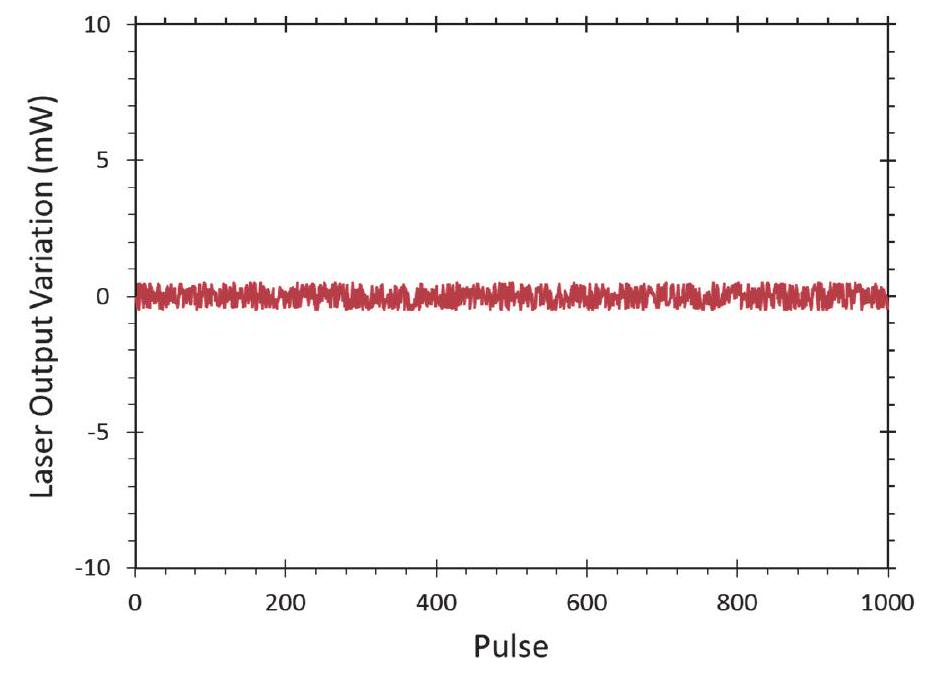
\includegraphics[max width=\textwidth]{2024_04_11_419211c3e451fc7cea07g-031}
\end{center}
\begin{center}
\includegraphics[max width=\textwidth]{2024_04_11_419211c3e451fc7cea07g-032(1)}
\end{center}
\begin{center}
\includegraphics[max width=\textwidth]{2024_04_11_419211c3e451fc7cea07g-032(3)}
\end{center}
\begin{center}
\includegraphics[max width=\textwidth]{2024_04_11_419211c3e451fc7cea07g-032(2)}
\end{center}
\begin{center}
\includegraphics[max width=\textwidth]{2024_04_11_419211c3e451fc7cea07g-032(4)}
\end{center}
\begin{center}
\includegraphics[max width=\textwidth]{2024_04_11_419211c3e451fc7cea07g-032(5)}
\end{center}
\begin{center}
\includegraphics[max width=\textwidth]{2024_04_11_419211c3e451fc7cea07g-032}
\end{center}

% (f)
(f)

中文:(f)

% Figure 4.4 Comparison of Monte Carlo simulations to an analytical model. ${ }^{17}$ The smooth (red) line is the equation and the jagged (blue) line is the Monte Carlo simulation results. Both vertical and horizontal comparisons between graphs are enabled by matching the $x$-axis and $y$-axis scales of every graph. Note that in this case redundant axes labels could be removed.
图4.4 蒙特卡洛模拟与解析模型的比较。${ }^{17}$ 平滑的(红色)线条表示方程,而锯齿状(蓝色)线条表示蒙特卡洛模拟的结果。通过匹配每个图的$x$轴和$y$轴的比例尺,可以在图形之间进行垂直和水平的比较。请注意,在这种情况下,可以删除多余的坐标轴标签。

% \subsection*{4.6 Figure Quality from a Production Standpoint}
\subsection*{从生产角度看的4.6图形质量}
% The final step in ensuring a good quality figure in your published paper is to make sure that the submitted figure matches the production requirements of the journal. (I speak here specifically about $\mathrm{JM}^{3}$ requirements, but I do not think they are much different from most other journals.) A few of the largest publications, such as Nature or Science, employ professional editors who can reset a graph to the standards of the journal. For most publications, however, it is up to the author to get the graph right. Below are some hints, given to me by the SPIE publications staff, that will make the production process go more smoothly and produce higherquality graphs:
确保您发表的论文中图形质量良好的最后一步是,要确保提交的图形符合期刊的生产要求。(我这里特别指的是$\mathrm{JM}^{3}$的要求,但我觉得它们与其他大多数期刊的要求并没有太大不同。)一些最大的出版物,如《自然》或《科学》,会雇佣专业编辑根据期刊的标准重置图表。然而,对于大多数出版物来说,责任在于作者自己确保图表正确。以下是由SPIE出版社工作人员提供的一些建议,这些将使生产过程更加顺利,并产生更高质量的图表:

\begin{itemize}
%   \item Submit high-resolution figures. The quality of the published figure is only as good as the original file - it cannot be improved by the typesetter. A resolution of $100 \mathrm{dpi}$ (dots per inch) looks great on a computer screen but is inadequate for print. A minimum of $300 \mathrm{dpi}$ is required, but $600 \mathrm{dpi}$ is preferred. Thus, a one-column wide photograph must be at least 1000 pixels across.
\item 提交高分辨率的图表。已发布的图表质量仅与原始文件的质量相当——排版人员无法提高其质量。$100 \mathrm{dpi}$(每英寸点数)在电脑屏幕上看起来不错,但对于印刷来说是不够的。至少需要$300 \mathrm{dpi}$,但更推荐$600 \mathrm{dpi}$。因此,一栏宽的照片横跨至少需要1000像素。
%   \item Submit full-size figures (7 in. wide), but remember that they will, in general, be reduced $50 \%$ to fit within one column. Make sure that the fonts, lines, and other elements of the graph will hold up to this reduction (see my font-size suggestions in the earlier Excel example). Try shrinking the graph 50\% and printing it out yourself as a test.
\item 提交全尺寸图表(宽7英寸),但请记住,它们通常会被缩小50%,以适应单栏的宽度。确保图表中的字体、线条和其他元素在小幅缩小后依然清晰可见(参考我之前Excel示例中的字体大小建议)。尝试将图表缩小50%,并自行打印出来作为测试。
%   \item High-contrast color graphics are great for online viewing, but the figures still need to be readable in grayscale for black-and-white printing (unless you pay for color printing). Colors such as red and blue, which are easy to distinguish online, are the same shade of gray when printed in black and white. If lines or symbols must be distinguished in a legend or caption, use different line styles and symbols instead of relying solely on color.
\item 高对比度的彩色图表非常适合在线观看,但图表在灰度模式下仍需要保持可读性,以便黑白打印(除非你支付彩色打印费用)。在线容易区分的红蓝色等,在黑白打印时会变成相同的灰度阴影。如果图例或标题中的线条或符号需要区分,应使用不同的线条样式和符号,而不是仅依赖于颜色。
%   \item Do not submit JPG files - the image compression often compromises the quality of the figure. TIF files have no compression, but if the file size is unmanageable try using "LZW" compression.
\item 不要提交JPG文件,因为图像压缩通常会损害图像的质量。TIF文件没有压缩,但如果文件大小无法控制,可以尝试使用“LZW”压缩。
%   \item If a figure contains multiple parts (such as Fig. 4.4), they should all be laid out in one file, not submitted as individual files. This is important because it lets the author determine how a figure should be arranged for the reader (horizontal versus vertical, for example). The parts should be clearly labeled with lowercase Roman text in parentheses, i.e., (a), (b), etc.
\item 如果一个图表包含多个部分(如图4.4),它们应该全部布局在同一个文件中,而不是作为单独的文件提交。这一点很重要,因为它让作者可以确定如何为读者安排图表的布局(例如,水平还是垂直)。各部分应该用小写的罗马数字文本加括号清晰地标注,即(a)、(b)等。
\end{itemize}

% \subsection*{4.7 Tables}
\subsection*{4.7 表格}
% Tables present data directly and are preferred over graphs when the exact numerical values of the data are needed. Still, tables often have a goal similar to that for figures: enabling comparisons. When presenting data in two or more dimensions, the layout and order of the table entries can make a huge difference in the ability of the reader to make the proper comparisons and see the important trends. It is easier for a reader to compare numbers arranged within a row than within a column. It is also easier to compare numbers that are close to each other (preferably next to each other).
表格直接呈现数据,当需要数据的准确数值时,它们比图表更受欢迎。然而,表格的目标通常与图表相似:便于比较。当以两个或更多维度呈现数据时,表格条目的布局和顺序对读者进行适当比较和识别重要趋势的能力有很大影响。读者更容易比较一行内的数字,而不是一列内的数字。比较彼此靠近的数字(最好是相邻的)也更容易。

% Often, 2D tables will benefit from marginal analysis, where rows and columns are totaled or expressed as a percentage of the total. The table in the next section shows an example of such marginal statistics.
通常,2D表格将受益于边际分析,这种分析会对行和列进行总计或表达为总量的百分比。下一节中的表格展示了此类边际统计的一个例子。

% As with figures, tables should be made comprehensible on their own, without reference to the text of the paper, if possible. This means that a table should have a good caption, and the items presented should be clearly defined within the table. Do not forget units and uncertainty estimates.
与图表一样,如果可能的话,表格应该能够独立于论文文本而让人理解。这意味着表格应该有一个好的标题,并且在表格内呈现的项目应该定义得非常清楚。不要忘记单位和不确定性估计。

% Different journals have different formatting requirements for tables. For example, many journals allow only horizontal lines in the table. Before submitting your manuscript, review the table formatting guidelines (or just look through the journal for examples of tables) and render your table in that format. A table arranged to look good in your preferred style may not work so well in the journals' required style.
不同的期刊对表格的格式要求各不相同。例如,许多期刊只允许在表格中使用水平线。在提交您的手稿之前,请查看表格格式指南(或直接浏览期刊中的表格示例),并将您的表格按照该格式进行排版。按照您个人喜好排版的表格可能不符合期刊所需的风格。

% \subsection*{4.8 Example: Figures and Tables in $\mathrm{JM}^{3}$}
\subsection*{4.8 示例:在 $\mathrm{JM}^{3}$ 中的图表和表格}
% How are graphs used in my journal, $\mathrm{JM}^{3}$ ? Table 4.1 shows my counts of figures and tables found in the 2012 issues of $\mathrm{JM}^{3}$. The graph types I used are somewhat arbitrary (as all categories are), but hopefully useful. $\mathrm{JM}^{3}$ papers in $2012 \mathrm{had}$ an average of 19 figures and one table per paper, attesting to the importance of figures in our field. About $20 \%$ of the figures were used to explain the theory or experimental setup, and the rest showed results. By far the most common figure was the ubiquitous $x-y$ plot, accounting for $1 / 3$ of all figures and tables. Results micrographs (optical and scanning electron micrographs, as well as atomic force microscope renderings) made up $25 \%$ of the figures. Contour and 3D plots were used about $10 \%$ of the time, with other types of charts filling in the remainder.
在我的期刊$\mathrm{JM}^{3}$中,图表是如何被使用的?表4.1显示了我对2012年$\mathrm{JM}^{3}$期刊中找到的图表和表格的统计计数。我所使用的图表类型有些随意(因为所有类别都是这样),但希望是有用的。2012年$\mathrm{JM}^{3}$的论文平均每篇有19个图表和一个表格,这证明了在我们领域中图表的重要性。大约$20 \%$的图表用于解释理论或实验设置,其余的展示了结果。最常见的图表是无所不在的$x-y$散点图,占所有图表和表格的$1/3$。结果显示显微图(光学显微图和扫描电子显微图,以及原子力显微镜渲染图)占了$25 \%$的图表。等高线和3D图的使用大约占$10 \%$,其余的图表类型填补了剩余部分。

% While I made no attempt to rate or judge the quality of the figures, it was clear to me from my survey that there were many excellent examples of figures and tables in all categories. There were some poor ones as well.
虽然我没有尝试去评价或判断图表的质量,但通过我的调查,很明显,在所有类别中都有许多优秀的图表和表格示例。也有一些质量较差的。

% As an exercise, I rendered the data from the "Results" figures of Table 4.1 into a variety of bar charts (see Fig. 4.5). Most of them fail the test of staying "on message." The first four draw attention to the variations between issues, either in actual numbers or in percentages, though the per-issue variation is not important to my story here. The last two correctly keep the emphasis on the relative frequency of each figure type, with the horizontal bar chart being far more
作为一种练习,我将表4.1中“结果”图的数据制作成了各种条形图(见图4.5)。其中大部分没有通过保持“信息一致”的测试。前四个图表突出了各问题之间的差异,无论是在实际数字还是百分比上,尽管这些问题之间的变化对于我这里的故事并不重要。最后两个图表正确地保持了每种图形类型的相对频率的强调,水平条形图在这方面要优越得多。

% Table 4.1 Figure and table counts for $\mathrm{JM}^{3}$ papers published in 2012.
表4.1 2012年发表的$\mathrm{JM}^{3}$论文中的图形和表格数量。

\begin{center}
\includegraphics[max width=\textwidth]{2024_04_11_419211c3e451fc7cea07g-028(1)}
\end{center}
\begin{center}
\includegraphics[max width=\textwidth]{2024_04_11_419211c3e451fc7cea07g-028}
\end{center}
\begin{center}
\includegraphics[max width=\textwidth]{2024_04_11_419211c3e451fc7cea07g-030}
\end{center}
\begin{center}
\includegraphics[max width=\textwidth]{2024_04_11_419211c3e451fc7cea07g-031}
\end{center}
\begin{center}
\includegraphics[max width=\textwidth]{2024_04_11_419211c3e451fc7cea07g-032(1)}
\end{center}
\begin{center}
\includegraphics[max width=\textwidth]{2024_04_11_419211c3e451fc7cea07g-032(3)}
\end{center}
\begin{center}
\includegraphics[max width=\textwidth]{2024_04_11_419211c3e451fc7cea07g-032(2)}
\end{center}
\begin{center}
\includegraphics[max width=\textwidth]{2024_04_11_419211c3e451fc7cea07g-032(4)}
\end{center}
\begin{center}
\includegraphics[max width=\textwidth]{2024_04_11_419211c3e451fc7cea07g-032(5)}
\end{center}
\begin{center}
\includegraphics[max width=\textwidth]{2024_04_11_419211c3e451fc7cea07g-032}
\end{center}
\begin{center}
\begin{tabular}{rrrrrrr}
 & Issue \#1 & Issue \#2 & Issue \#3 & Issue \#4 & Total & \% of Total \\
\begin{tabular}{r}
No. Papers \\
Methods \\
\end{tabular} & 24 & 43 & 22 & 12 & 101 &  \\
Photos &  &  &  &  &  &  \\
Diagrams & 92 & 120 & 85 & 25 & 322 & $\mathbf{1 6 . 3 \%}$ \\
Tables & 6 & 11 & 4 & 12 & 33 & $\mathbf{1 . 7 \%}$ \\
\cline{ 2 - 7 }
Setup Total & 109 & 187 & 96 & 40 & 432 & $\mathbf{2 1 . 9 \%}$ \\
Results &  &  &  &  &  &  \\
x-y Plots & 138 & 281 & 120 & 114 & 653 & $\mathbf{3 3 . 1 \%}$ \\
Contour Plots & 47 & 52 & 25 & 62 & 186 & $\mathbf{9 . 4 \%}$ \\
3D Plots & 2 & 10 & 17 & 13 & 42 & $\mathbf{2 . 1 \%}$ \\
Micrographs & 89 & 131 & 222 & 40 & 482 & $\mathbf{2 4 . 4 \%}$ \\
Histograms & 6 & 6 & 4 & 0 & 16 & $\mathbf{0 . 8 \%}$ \\
Bar Charts & 10 & 2 & 4 & 11 & 27 & $\mathbf{1 . 4 \%}$ \\
Wafer Maps & 6 & 0 & 1 & 1 & 8 & $\mathbf{0 . 4 \%}$ \\
Tables & 25 & 53 & 23 & 10 & 111 & $\mathbf{5 . 6 \%}$ \\
Other & 6 & 4 & 3 & 4 & 17 & $\mathbf{0 . 9 \%}$ \\
\cline{ 2 - 7 }
Results Total & 329 & 539 & 419 & 255 & 1542 & $\mathbf{7 8 . 1 \%}$ \\
\cline{ 2 - 7 }
\end{tabular}
\end{center}

\begin{center}
\includegraphics[max width=\textwidth]{2024_04_11_419211c3e451fc7cea07g-028(1)}
\end{center}
\begin{center}
\includegraphics[max width=\textwidth]{2024_04_11_419211c3e451fc7cea07g-028}
\end{center}
\begin{center}
\includegraphics[max width=\textwidth]{2024_04_11_419211c3e451fc7cea07g-030}
\end{center}
\begin{center}
\includegraphics[max width=\textwidth]{2024_04_11_419211c3e451fc7cea07g-031}
\end{center}
\begin{center}
\includegraphics[max width=\textwidth]{2024_04_11_419211c3e451fc7cea07g-032(1)}
\end{center}
\begin{center}
\includegraphics[max width=\textwidth]{2024_04_11_419211c3e451fc7cea07g-032(3)}
\end{center}
\begin{center}
\includegraphics[max width=\textwidth]{2024_04_11_419211c3e451fc7cea07g-032(2)}
\end{center}
\begin{center}
\includegraphics[max width=\textwidth]{2024_04_11_419211c3e451fc7cea07g-032(4)}
\end{center}
\begin{center}
\includegraphics[max width=\textwidth]{2024_04_11_419211c3e451fc7cea07g-032(5)}
\end{center}
\begin{center}
\includegraphics[max width=\textwidth]{2024_04_11_419211c3e451fc7cea07g-032}
\end{center}
\begin{center}
\begin{tabular}{rrrrrrr}
 & Issue \#1 & Issue \#2 & Issue \#3 & Issue \#4 & Total & \% of Total \\
\begin{tabular}{r}
No. Papers \\
Methods \\
\end{tabular} & 24 & 43 & 22 & 12 & 101 &  \\
Photos &  &  &  &  &  &  \\
Diagrams & 92 & 120 & 85 & 25 & 322 & $\mathbf{1 6 . 3 \%}$ \\
Tables & 6 & 11 & 4 & 12 & 33 & $\mathbf{1 . 7 \%}$ \\
\cline{ 2 - 7 }
Setup Total & 109 & 187 & 96 & 40 & 432 & $\mathbf{2 1 . 9 \%}$ \\
Results &  &  &  &  &  &  \\
x-y Plots & 138 & 281 & 120 & 114 & 653 & $\mathbf{3 3 . 1 \%}$ \\
Contour Plots & 47 & 52 & 25 & 62 & 186 & $\mathbf{9 . 4 \%}$ \\
3D Plots & 2 & 10 & 17 & 13 & 42 & $\mathbf{2 . 1 \%}$ \\
Micrographs & 89 & 131 & 222 & 40 & 482 & $\mathbf{2 4 . 4 \%}$ \\
Histograms & 6 & 6 & 4 & 0 & 16 & $\mathbf{0 . 8 \%}$ \\
Bar Charts & 10 & 2 & 4 & 11 & 27 & $\mathbf{1 . 4 \%}$ \\
Wafer Maps & 6 & 0 & 1 & 1 & 8 & $\mathbf{0 . 4 \%}$ \\
Tables & 25 & 53 & 23 & 10 & 111 & $\mathbf{5 . 6 \%}$ \\
Other & 6 & 4 & 3 & 4 & 17 & $\mathbf{0 . 9 \%}$ \\
\cline{ 2 - 7 }
Results Total & 329 & 539 & 419 & 255 & 1542 & $\mathbf{7 8 . 1 \%}$ \\
\cline{ 2 - 7 }
\end{tabular}
\end{center}
\begin{center}
\begin{tabular}{rrrrrr}
\begin{tabular}{r}
Tables and \\
Figures Total \\
Tables and \\
\end{tabular} & 438 & 726 & 515 & 295 & 1974 \\
\begin{tabular}{r}
Figures/Pape \\
\end{tabular} &  &  &  &  &  \\
$\mathbf{r}$ & $\mathbf{1 8 . 3}$ & $\mathbf{1 6 . 9}$ & $\mathbf{2 3 . 4}$ & $\mathbf{2 4 . 6}$ & $\mathbf{1 9 . 5}$ \\
\end{tabular}
\end{center}

% aesthetically pleasing. But then, they do not do a better job of conveying the message compared to the table, and the table is far richer and denser in information (and has the added benefit of documenting the data better). This conclusion is quite frequently true of bar charts: a table would be better.
美观悦目。但随后,它们在传达信息方面并不比表格做得更好,而且表格在信息上要丰富和密集得多(而且有更好的记录数据的附加好处)。这个结论对于条形图来说通常是正确的:表格会更好。

% \subsection*{4.9 Conclusions}
\subsection*{4.9 结论}
% When presenting results, a good graph is like a good scientific theory: once you see it, everything just makes sense. But arriving at such a point takes care and consideration. Keeping in mind the advice from this chapter will, I hope, lead to graphs that help you, the author, achieve your goal of effective and efficient communication.
在展示结果时,一个好的图表就像一个好的科学理论:一旦你看到它,一切都会变得很有道理。但是达到这样的效果需要细心和考虑。记住本章中的建议,我希望这能引导你,作为作者,实现有效且高效的沟通目标。
\includegraphics[max width=\textwidth, center]{2024_04_11_419211c3e451fc7cea07g-036}

% Figure 4.5 A comparison of six different bar charts based on the data from the "Results" section of the table. The top four graphs are "off-message," emphasizing the per-issue variation. The bottom two have the proper emphasis but are not very data-dense.
图4.5显示了基于表格“结果”部分数据绘制的六种不同条形图的比较。前四个图表强调议题的差异性,是“偏离要点的”。而最后两个图表虽然强调了正确的部分,但数据密度不高。

% They say a picture is worth a thousand words. In a scientific journal, each figure occupies the space of anywhere from 150 to 500 words. So at the very least, a figure should convey more information than the words it displaces. Otherwise, valuable space has been wasted. A good graph can certainly do that, though not all figures do. As the abstract artist Ad Reinhardt so aptly put it, "As for a picture, if it isn't worth a thousand words, the hell with it."
他们说一张图片胜过千言万语。在科学期刊中,每一幅图表所占的空间相当于150到500个单词。因此,至少图表应该传达出它所占空间单词以上的信息,否则就是浪费了宝贵的空间。一幅好的图表无疑能做到这一点,但并非所有图表都能做到。正如抽象艺术家阿德·莱因哈特精辟地所说:“至于一幅画,如果它连一千个字都不值,那就算了吧。”

% \section*{References}
\section*{参考文献}
${ }^{1}$ E. R. Tufte, The Visual Display of Quantitative Information, Graphics Press, Cheshire, CT, p. 6 (1983).

${ }^{2}$ J. W. Tukey, Exploratory Data Analysis, Addison-Wesley, Reading, MA (1977).

${ }^{3}$ W. S. Cleveland, "Graphs in Scientific Publications", The American Statistician 38(4), 261-269 (Nov. 1984).

${ }^{4}$ E. R. Tufte, Visual Explanations, Graphics Press, Cheshire, CT, p. 43 (1997).

${ }^{5}$ M. Kozak, "Basic principles of graphing data", Sci. Agric. 67(4), 483-494 (July/August 2010).

${ }^{6}$ E. R. Tufte, Visual Explanations, Graphics Press, Cheshire, CT, p. 53 (1997).

${ }^{7}$ ibid., p. 70.

${ }^{8}$ W. S. Cleveland, The Elements of Graphing Data, Wadsworth \& Brooks/Cole, Pacific Grove, CA (1985).

${ }^{9}$ E. R. Tufte, The Visual Display of Quantitative Information, Graphics Press, Cheshire, CT, p. 77 (1983).

${ }^{10}$ ibid., p. 168.

${ }^{11}$ W. S. Cleveland, The Elements of Graphing Data, Wadsworth \& Brooks/Cole, Pacific Grove, CA, p. 57 (1985).

% 12 J. W. Tukey, Exploratory Data Analysis, Addison-Wesley, Reading, MA (1977).
J. W. 图基,《探索性数据分析》,艾迪生·卫斯理出版社,马萨诸塞州雷丁(1977年)。

${ }^{13}$ M. Friendly and D. Denis, "The Early Origins and Development of the Scatterplot", $J$. History Behavioral Sci. 41(2), 103-130 (Spring 2005).

${ }^{14}$ J. F. W. Herschel, "On the investigation of the orbits of revolving double stars", Memoirs Royal Astronomical Soc. 5, 171-222 (1833).

${ }^{15}$ The Oxford English Dictionary, $2^{\text{nd }}$ ed., Oxford Univ. Press (1989).

${ }^{16}$ C. A. Mack, "Systematic Errors in the Measurement of Power Spectral Density", $J$. Micro/Nanolithography, MEMS, and MOEMS 12(3), 033016 (Jul-Sep, 2013).

${ }^{17}$ B. D. Bunday and C. A. Mack, "Influence of Metrology Error in Measurement of Line Edge Roughness Power Spectral Density”, Proc. SPIE 9050, 90500G (2014).

% \section*{Chapter 5}
\section*{第五章}
% \section*{Citations}
\section*{引文/引用}
% As described in the Preface, the growth of scientific knowledge is predominately incremental - we build on past knowledge more often than we displace it. Thus, the first pillar of science-a communal collection of knowledge-requires mechanisms for preserving and disseminating knowledge within the scientific community. By far the most important mechanism in use today is the scientific publication. Although there are many forms of scientific publication, the two most common are the conference presentation (with or without some non-peer-reviewed written text) and the peer-reviewed journal paper (both in print and online).
正如前言所述,科学知识的增长主要是递增的——我们更多地是在过去的知识基础上进行构建,而不是取代它。因此,科学的第一支柱——共同的知识集合——需要机制来在科学界内保存和传播知识。到目前为止,今天使用的最重要的机制就是科学出版物。尽管科学出版物有许多形式,但最常见的两种是会议报告(可能带有一些非同行评审的书面文本)和同行评审的期刊论文(包括印刷版和在线版)。

% Because virtually all scientific advances build on past knowledge, it is critical that the new work be placed in the proper context with respect to the past work upon which it builds. The primary mechanism for this is the citation (or reference). Within a scientific paper, references are placed to other works, creating points of contact with the communal collection of scientific literature in order to fit the new work into the web of knowledge. But given the skeptical attitude that is also a part of science, citations are also used to help readers verify the quality of the new work and assess the strength of its conclusions.
由于几乎所有的科学进步都是建立在过去的知识基础之上的,因此将新工作与其所依赖的过去工作置于适当的背景中至关重要。实现这一目标的主要机制是引用(或参考文献)。在科学论文中,参考文献指向其他作品,与科学文献的共同集合建立联系,以使新工作融入知识网络。但鉴于科学中也存在怀疑的态度,引用还用于帮助读者验证新工作的质量,并评估其结论的强度。

% \subsection*{5.1 The Five Goals of Citations}
\subsection*{5.1 引用的五个目标}
% A citation is, by definition, a reference to a source of information or data. Things that can be cited include journal articles, conference proceedings, books, student theses, newspapers, non-print sources (such as film or other recorded media), websites or other online resources, computer materials (such as a published CDROM of data or a piece of software), and personal communications. The citation should be located in the text in such a way that it is clear what material requires the citation. Often, this is at the end of a sentence, but sometimes it must be put in the middle of the sentence to enhance clarity. Obviously, citations must supply sufficient detail so that the referenced material can be found and uniquely identified. As such, every journal establishes a specific format for citations that must be followed. (Alas, there is no universal format that all journals follow.)
引文,按定义,是对信息或数据来源的引用。可以引用的内容包括期刊文章、会议论文集、书籍、学生论文、报纸、非印刷来源(如电影或其他记录媒介)、网站或其他在线资源、计算机材料(如发布的数据CD-ROM或一片软件),以及个人通讯。引文应该在文本中的位置明确指出哪些内容需要引用。通常,这位于句子的末尾,但有时为了增强清晰性,必须将引文放在句子的中间。显然,引文必须提供足够的细节,以便能够找到并唯一确定所引用的材料。因此,每个期刊都建立了特定的引文格式,必须遵守。(遗憾的是,并非所有期刊都遵循统一的格式。)

% Though simple in concept, citations in a scientific paper serve many goals. The five most important goals are
虽然概念上很简单,但科学论文中的引用服务于许多目标。最重要的五个目标是:

\begin{itemize}
%   \item Provide sufficient context of the work to allow for critical analysis of the work by others and thus to enable the readers to gauge for themselves whether the author's conclusions are justified;
\item 提供足够的作品背景,以便他人对作品进行批判性分析,从而使读者能够自行判断作者的结论是否站得住脚。
%   \item Give the reader sources of background and related material so that the current work can be understood by the target audience (thus creating a web of science);
\item 向读者提供背景资料和相关材料的来源,以便目标受众能够理解当前的工作(从而构建一个科学网络)。
%   \item Establish credibility with the reader (e.g., the authors knows the field, have done their homework, etc.) and/or inform the reader that the paper belongs within a specific school of thought;
\item 与读者建立信誉(例如,作者了解该领域,已经做好准备工作等)和/或通知读者该论文属于特定的学派思想。
%   \item Provide examples of alternate ideas, data, or conclusions to compare and contrast with this work; and
\item 提供一些替代想法、数据或结论,以便与这项工作进行比较和对比;并
%   \item Acknowledge and give credit to sources relied upon for this work (i.e., acknowledge the use of another's ideas or data), thus upholding intellectual honesty.
\item 确认并给予依赖于此工作所引用的来源(即,确认使用了他人的想法或数据),从而维护学术诚信。
\end{itemize}

% Of these five goals, the most commonly mentioned is to give credit to others (the so-called normative theory of citations ${ }^{1}$ ) and thus demarcate what credit is due the new work. In truth, scientists can have big egos. We are frequently motivated by the desire for peer recognition. Thus, we try to carefully stake a claim to new ideas or data in our paper, knowing full well that others will be checking to make sure we do not claim too much. Even so, there is no pretense that a list of references will provide a complete list of influences; such a list would be excessive in even the simplest of cases.
这五个目标中,最常被提及的是给予他人认可(所谓的引证规范理论${ }^{1}$),从而界定新作品应得的认可。实际上,科学家可能都有很强的自尊心。我们经常是由对同行认可的渴望所驱动。因此,我们在论文中试图小心翼翼地主张新的观点或数据,清楚地知道其他人会检查以确保我们不会要求过多。即便如此,没有假装参考文献列表就能提供完整的影响清单;即使在最简单的情况下,这样的列表也会过于冗长。

% While important, the "give credit" purpose of citations is, in my opinion, less compelling than the other goals. I view citations, like all aspects of scientific writing, from a simple perspective: what best serves the needs of the reader? Thus, the primary goal of citations should be to help the reader gain the most from the paper. Imagine your paper being read by graduate students or postdocs: smart, but new to the field. If they read all of the citations, will they have enough background to understand your work? Will any of the references be unneeded or redundant (and thus a waste of the reader's time)? Chances are very good that a simple test will be sufficient to decide on most references: will adding this reference here make the paper more valuable to the reader, or less?
虽然重要,但在我看来,引用的“给予信用”的目的不如其他目标那么有说服力。我从一个简单的角度来看待引用,就像科学写作的所有方面一样:什么最能满足读者的需求?因此,引用的主要目标应该是帮助读者从论文中获得最多的信息。想象一下你的论文被研究生或博士后阅读:他们聪明,但对这个领域来说是新手。如果他们阅读了所有的引用,他们是否会有足够的背景来理解你的工作?是否有任何参考文献会是多余的(从而浪费读者的时间)?很有可能,一个简单的测试就足以决定大多数参考文献:在这里添加这个参考文献是否会增加论文对读者的价值,还是减少?

% \subsection*{5.2 The Literature Search}
\subsection*{5.2 文献检索}
% A new research project almost always begins with a literature search, as discussed in Chapter 1. Thus, you should have a good idea what the key papers in the field are before you begin the research. This literature search should be updated during your research, especially as new ideas come or directions change. A review of your literature search results just before you begin drafting your manuscript will allow you to cite as you write. Also, other researchers are often working on similar topics and may have published papers after your original literature search was completed.
一个新的研究项目几乎总是从文献检索开始,正如第一章所讨论的。因此,在开始研究之前,你应该对领域内的关键论文有一个很好的了解。在你的研究过程中,应该更新文献检索,特别是当有新的想法出现或研究方向改变时。在开始撰写手稿之前,回顾一下你的文献检索结果,将使你在写作时能够直接引用。此外,其他研究者通常也在研究类似的主题,并且可能在你的原始文献检索完成之后发表了新的论文。

% A common mistake is to save the literature search until the end of the paper writing process. Doing a literature search only at the end often generates spurious citations (a problem that will be discussed in Section 5.4) and rarely provides the most valuable citations.
一个常见的错误是在论文写作过程快结束时才进行文献搜索。只在最后进行文献搜索常常会产生错误的引用(这个问题将在第5.4节讨论),而且很少能提供最有价值的引用。

% \subsection*{5.3 Verify, Verify, Verify}
\subsection*{5.3 验证,验证,验证}
% One of the most pervasive problems with citations is that they are frequently incomplete or inaccurate. It is the job of the authors to verify the accuracy of the references. Editors, copyeditors, and reviewers are not responsible for reference accuracy and are not expected to check references for accuracy. And though copyeditors try to flag incomplete or improperly formatted references, it is the authors who must ultimately fix the errors found. Why not do the work up front to ensure that the references are complete, accurate, and properly formatted? It will only save time and effort in the end, and indicate to the editors and reviewers that you care enough to pay attention to these important details.
引用中最为普遍的问题之一是它们常常不完整或准确。作者有责任核实参考文献的准确性。编辑、文字编辑和审稿人并不负责参考文献的准确性,也不期望他们去检查引用是否准确。尽管文字编辑会尝试标出不完整或格式不正确的引用,但最终必须由作者来纠正发现的错误。为什么不一开始就做好工作,确保引用完整、准确并且格式正确呢?这最终只会节省时间和精力,并向编辑和审稿人表明你足够重视这些重要的细节。

% Alas, far too few authors take this advice seriously. Several studies have found that between 34 and $67 \%$ of references in a variety of medical and biomedical journals contained errors. ${ }^{2}$ These errors can be broken down into major and minor errors. A major error means that the article could not be found given the information in the citation. One study found that major errors occur in $7 \%$ of the citations from one class of medical journals. ${ }^{3}$ Minor errors include punctuation or spelling mistakes, mistakes in the article titles, mistakes in the name and initials of the author(s), and citation style mistakes. These errors serve as irritants to the reader-they can still find the article, but they have to put more effort into it.
唉,太少有作者认真采纳这些建议。几项研究发现,在各类医学和生物医学期刊中,有34%至67%的参考文献包含错误。②这些错误可以分为主要错误和次要错误。主要错误是指根据引用信息找不到文章。一项研究发现,在一类医学期刊的引用中,有7%存在主要错误。③次要错误包括标点或拼写错误、文章标题错误、作者(们)的名字和首字母错误以及引用格式的错误。这些错误对读者来说是一种刺激——他们仍然能找到文章,但必须付出更多努力。

% It is probably obvious that the main cause of errors in citations is simple sloppiness on the part of the author. There is another problem, however, that may also be at work: copying citations from other papers. In other words, some authors commit a cardinal sin of citations and add a reference without ever having read that paper. Copying citations from other papers without actually looking up and reading that paper can result in a propagation of errors that are never corrected ${ }^{4}$ (like a children's game of "telephone"). A slightly less egregious form is the abstract citation: citing a paper after reading only the abstract. Both types of unread citation should be avoided: cite only papers you have read.
很明显,引用错误的主要原因在于作者的粗心大意。然而,可能还存在另一个问题:即从其他论文中复制引用。换句话说,一些作者在引用时犯了一个大忌,他们在从未读过某篇论文的情况下就添加了参考文献。从其他论文中复制引用,而没有实际查阅和阅读该论文,可能导致错误的传播,而这些错误永远不会被纠正(就像孩子们玩的“传话”游戏)。稍微不那么严重的做法是摘要引用:只阅读摘要后即引用一篇论文。应避免这两种未阅读的引用方式:只引用你真正阅读过的论文。

% \subsection*{5.4 Other Problems with Citations}
\subsection*{5.4 引文的其他问题}
% There are other reasons why a specific reference does not fulfill the goals set out here and thus does not benefit the reader.
这里有其他原因说明为什么特定的参考没有达到此处所设定的目标,因此也没有对读者产生益处。

% Spurious citations: citations that are not needed but are included anyway. These citations are sometimes added at the last minute, after the paper is written, to give the impression that a literature search and proper citation work have been done. They often include redundant citations, where the extra citations do not add any value beyond the first one. A simple example was given by Brian Thompson: ${ }^{5}$ "related work on the technique has been carried out by numerous researchers. ${ }^{1-101 \text{ ", }}$ The problem is obvious: an interested reader must wade through far too muc literature to get the needed background. Sometimes spurious cites are meant to give an impression of erudition by citing an obscure, historical reference (if the referenced work is in a foreign language, all the better).$^{6}$ In all such cases, simply asking the question "If the reader looks up this reference, will it be time well spent?" will be enough to decide if that reference is spurious.
虚假引用:这些引用并不必要,但仍然被包含在内。有时这些引用是在论文写完后的最后一分钟添加的,以给人已经进行了文献搜索和适当引用工作的印象。它们常常包括多余的引用,额外的引用并没有比第一个引用增加任何价值。Brian Thompson给出了一个简单的例子:${ }^{5}$ "有许多研究者对这项技术进行了相关研究。${ }^{1-101 \text{ "}}$ 问题很明显:感兴趣的读者必须浏览过多的文献才能获得所需背景知识。有时虚假引用是为了给人博学的印象而引用一个晦涩的历史文献(如果引用的工作是用外语写的,那就更好了)。$^{6}$ 在所有这类情况下,只需问一个问题 "如果读者查阅这个参考文献,这会是一段时间的好花费吗?" 就足以判断那个引用是否是虚假的。

% Biased citations: references added (or omitted) for reasons other than meeting the five goals of citations. Biases include overciting of friends' or colleagues' work, omitting cites to the work of rivals, and gratuitous citations in an attempt to curry favor with a boss or potential referee.
引用偏差:出于除了满足引用的五个目标之外的其它原因而添加(或省略)的参考文献。偏差包括过度引用朋友或同事的工作,省略对竞争对手工作的引用,以及为了讨好上司或潜在评审人而进行的无必要引用。

% Self-cites: citations to one's own work. There is nothing wrong with selfcitations, per se. After all, the work represented in a single paper is often just the latest result of a larger ongoing project. As such, citations to one's earlier work are often perfectly appropriate and sometimes required. Self-cites are a problem when they are either spurious or biased. ${ }^{7}$ Knowing as we do the tendencies of many scientists toward self-promotion, one fears that self-cites may be designed to boost the recognition of the author rather than increase the value of the paper to the reader.
自引:引用自己的作品。自引本身并没有问题。毕竟,一篇论文中的工作往往只是更大正在进行项目中的最新成果。因此,引用自己之前的作品通常是完全恰当的,有时甚至是必要的。自引成为问题是在它们要么是虚假的,要么是带有偏见的时候。${ }^{7}$ 众所周知,许多科学家倾向于自我推销,人们担心自引可能是为了提高作者的知名度,而不是增加论文对读者的价值。

% Excluding contrary evidence: a form of biased citations where citations to prior work whose conclusions or data contradict the current work are omitted. Because one of the five goals of citations is to explicitly contrast the new work with prior work containing conflicting data or conclusions, avoiding such conflict (for whatever reason) does not serve the interest of science.
排除相反证据:一种引用偏差的形式,其中省略了对先前工作的引用,这些工作的结论或数据与当前工作相矛盾。因为引用的五个目标之一是明确地将新工作与包含相冲突数据或结论的先前工作进行对比,所以无论出于何种原因避免这种冲突,都不符合科学利益。

% In the end, authors must find a balance between too many and too few citations. The literature base even on vary narrow topics is often vast, and it can be difficult to pick a small subset to cite. In general, authors can mitigate citation problems by asking two questions:
最终,作者必须在引用过多和过少之间找到平衡。即便是非常狭窄的课题,文献基础往往也是庞大的,从中挑选出一小部分进行引用可能会很难。一般来说,作者可以通过问自己两个问题来缓解引用的问题:

% "Have I provided the references that will make this paper as useful as possible?" "If the reader looks up a given reference, will it be time well spent?"
"我是否提供了能让这篇论文尽可能有用的参考文献?”“如果读者查阅了一个特定的参考文献,这会是值得的吗?”

% \subsection*{5.5 More on Self-Citations}
\subsection*{5.5 更多关于自引引用的内容}
% Citations sometimes have significance for reasons other than the five listed above. Citations can be counted, and in a data-driven world these counts have assumed outsized importance as a proxy for the influence of a given paper. Citation counts serve as (flawed) measures of journal importance (the impact factor) and researcher clout (the h-index, among other metrics). Today, such citation counts and their metrification are used in hiring and promotion decisions, especially in academia, often as a substitute for thoughtful and informed judgment.
引用有时因上述五个原因之外的其他因素而具有意义。引用可以被统计,在一个数据驱动的世界里,这些统计数字作为衡量一篇给定论文影响力的代理而变得格外重要。引用次数作为(有缺陷的)衡量期刊重要性(影响因子)和研究人员影响力(h指数以及其他指标)的指标。如今,这样的引用次数及其量化在招聘和晋升决策中被广泛使用,尤其是在学术界,常常替代深思熟虑和有根据的判断。

% Be careful what you measure, because a truism of the business world is 'what gets measured gets managed'. And measures that come with rewards often get gamed. When a person's career or reputation depends on citation counts, the temptation to inflate those counts is never far away. Some authors are more likely to cite their colleagues' work than their competitors'; some journals expect their submitting authors to preferentially cite work published in that journal. But th easiest way to promote your own work (and thus yourself) is with the self-citation: a citation to one's own prior work.
要小心你衡量的事物,因为商业世界的一条真理就是“被衡量的事物将被管理”。而伴随着奖励的衡量指标常常会被操纵。当一个人的职业或声誉取决于引用次数时,膨胀那些次数的诱惑就近在咫尺。一些作者更可能引用同事的工作而非竞争对手的;一些期刊期望其投稿作者优先引用该期刊发表的作品。但提升自己工作(从而提升自己)最简单的方法就是自我引用:即引用自己之前的工作。

% Self-cites are not inherently problematic. Most scientific publications describe a part of a longer-term research effort, and self-citations can put the new publication in the context of that larger effort. Self-cites become a problem only when they are either spurious or biased. Because deciding that a specific citation is either spurious or biased requires a judgement based on the cited work, the paper in which the citation occurs, and the field within which the work resides, it is not always an easy evaluation to make. Some cases are obvious, as when a majority of a research paper's citations are to the author's own work in a popular field of research. Other cases are less obvious, as when the authors are nearly the only ones working on a very specialized topic. Still, I think most authors know when they are pushing into spurious or biased territory with their self-citations. So the best defense against abuse is self-regulation.
自引并不本质上是有问题的。大多数科学出版物描述的是一个长期研究努力的一部分,自引可以将新的出版物放在这个更大努力的背景之中。只有当自引是虚假的或者有偏见的时,才会成为问题。因为判断一个特定的引用是否虚假或者有偏见需要基于被引用的工作、引用发生的论文以及工作所在领域进行判断,所以这并不总是容易评估的。有些情况是明显的,比如当一个研究论文的大部分引用都是作者在热门研究领域对自己的工作的引用时。其他情况则不太明显,比如当作者是在一个非常专业的主题上几乎唯一的研究者时。不过,我认为大多数作者都知道他们在自引时何时进入了虚假或有偏见的领域。因此,防止滥用最好的防御是自我调节。

% Or is it? An interesting study commissioned by the Chronicle of Higher Education looked at the role of gender in self-citation rates. ${ }^{8}$ An examination of 1.7 million $J S T O R$ papers spanning disciplines and over 60 years found that nearly $10 \%$ of citations were self-citations. Further analysis showed that men were $56 \%$ more likely to cite their own work than women, with the gender disparity growing over time. Apparently, self-regulation of self-citations is more effective in women than men.
或者是这样吗?《高等教育纪事报》委托进行的一项有趣的研究,探讨了性别在自引率中的作用。\textsuperscript{8} 对跨越多个学科、时间跨度超过60年的170万篇$JSTOR$论文的检查发现,近$10\%$的引用是自引。进一步的分析显示,男性引用自己作品的频率比女性高出$56\%$,而且这种性别差异随时间增长。显然,在自引的自我调节方面,女性比男性更为有效。

% What is the cause of this gender disparity? Women in academia seem less inclined to self-promotion than men, probably to their detriment. Does society pressure women to be more "feminine" and modest about their accomplishments? Are men encouraged to be more aggressive in pursuit of career success? Do women work on smaller teams with fewer publications and fewer opportunities for selfcitations? I am certainly not qualified to address such heady questions, but regardless of cause the issue of gender disparity in self-citations has consequences.
这种性别差异的原因是什么?学术界的女性似乎比男性更不愿意自我推销,这可能会对她们不利。是不是社会压力使女性更加“女性化”和谦逊,对自己的成就轻描淡写?是不是鼓励男性在追求职业成功时更加积极进取?女性是不是在更小的团队工作,发表的论文较少,自我引用的机会也较少?我当然没有资格回答这些深刻的问题,但无论原因如何,自我引用中的性别差异问题都带来了后果。

% In the age of Big Data, success breeds success, and popularity snowballs. The most linked webpages, the most watched videos, and the most downloaded journal papers are "recommended" or promoted to website visitors and social media consumers, generating a handful of winners-take-all and a long tail of neglected also-rans. The bandwagon effect seems true in the world of academic citations as well. Could it be that even modest differences in self-citation rates might snowball into noticeable differences in total citations? In other words, does self-promotion through self-citation work?
在大数据时代,成功孕育成功,人气滚雪球般增长。链接最多的网页、观看次数最多的视频以及下载次数最多的期刊论文会被“推荐”给网站访问者和社会媒体用户,形成了少数赢家通吃的局面,以及一大群被忽视的落后者。这种跟风效应在学术论文引用的世界中似乎也成立。是不是即使是自我引用率上的微小差异,也可能滚雪球般地导致总引用次数上明显的差异呢?换句话说,通过自我引用进行自我推广真的有效吗?

% One 2007 study showed that it does, with each self-citation multiplying into three other citations to that author over a five-year period. ${ }^{9}$ Further, the penalties for excessive self-citation seem to be small or none. Although this study looked at papers published from 1981-2000, I imagine that the higher levels of online searching and reading today have only increased this multiplying effect. Differences in self-citation rates are likely only one of many factors contributing to gender disparities in academic careers, but it may be one of the easier ones to address.
2007年的一项研究表明,确实如此,每篇自我引用在五年内会转化为对该作者的三篇其他引用。${ }^{9}$此外,过度自我引用的惩罚似乎很小或根本不存在。尽管这项研究考察的是1981-2000年间发表的文章,我想象如今更高水平的在线搜索和阅读只会增加这种倍增效应。自我引用率的差异很可能是导致学术界性别差异的众多因素之一,但可能是其中较容易解决的一个。

% Proper citations require careful consideration of the appropriate goals of citations, aided by a simple ethos: make the paper reader-centric, not authorcentric. Self-promotion is an author-centered way of looking at the activity of publishing, and it is neither good nor bad when considering the needs of the reader. Though self-cites should not be added to a paper solely for self-promotion, neither should self-cites be avoided for fear that they might appear self-promoting and thus unseemly. By focusing on the reader and the five proper goals of citations, most problems concerning citations can be easily avoided.
恰当的引用需要仔细考虑引用的适当目标,这一点可以通过一个简单的原则来辅助:使论文以读者为中心,而不是以作者为中心。自我推广是一种以作者为中心的看待出版活动的方式,在考虑读者需求时,这既不是好的也不是坏的。尽管不应该仅仅为了自我推广而向论文中添加自引,但也不应该因为担心自引看起来像是自我推广而避讳自引。通过关注读者和引用的五个适当目标,大多数关于引用的问题都可以轻松避免。

% \subsection*{5.6 Conclusions}
\subsection*{5.6 结论}
% To do a good job of providing citations in a scientific publication, one must keep in mind the multiple goals of proper citing. But like other aspects of good scientific writing, a simple theme has emerged: make the paper reader-centric, not authorcentric. Although it is common to choose citations that make the paper more valuable to the author (by demarcating what is novel, for example), good citations make the paper more valuable to the reader. Unfortunately, doing a good job of citing requires more work from the authors. But careful citing is worth the effort if your goal is a quality scientific publication.
要在科学出版物中提供引用方面做好工作,必须牢记适当引用的多个目标。但与良好科学写作的其他方面一样,一个简单的主题已经显现出来:应将论文以读者为中心,而非以作者为中心。尽管选择那些使论文对作者更有价值的引用很常见(例如,通过标示什么是新颖的),但好的引用应使论文对读者更有价值。不幸的是,如果想要做好引用工作,作者需要付出更多努力。但如果您的目标是高质量的科学研究出版物,那么仔细引用是值得努力的。

% \section*{References}
\section*{参考文献}
\myfootnote{${ }^{1}$ R. K. Merton, The Sociology of Science: Theoretical and Empirical Investigations, University of Chicago Press, Chicago, IL (1973).
}
\myfootnote{${ }^{1}$ R. K. Merton, The Sociology of Science: Theoretical and Empirical Investigations, University of Chicago Press, Chicago, IL (1973).

${ }^{2}$ T. S. Kuhn, The Structure of Scientific Revolutions, 3rd ed., University of Chicago Press, Chicago, IL (1996).

${ }^{3}$ Editorial, "Go forth and replicate!", Nature 536, 373 (2016).

${ }^{4}$ F. C. Fang and A. Casadevall, "Competitive Science: Is Competition Ruining Science?", Infection and Immunity 83(4), 1229 (2015).
}
\myfootnote{${ }^{1}$ J. M. Swales, Genre Analysis: English in Academic and Research Settings, pp. 140-166, Cambridge University Press, Cambridge, England (1990).

${ }^{2}$ L. F. Azevedo et al., "How to write a scientific paper - Writing the methods section", Rev. Port. Pneumol. 17(5), 232-238 (2011).

${ }^{3}$ J. M. Swales, Genre Analysis: English in Academic and Research Settings, 172-173, Cambridge University Press, Cambridge, England (1990).
}
\myfootnote{${ }^{1}$ F.-N. Thomas and M. Turner, Clear and Simple as the Truth: Writing Classic Prose, Princeton University Press, Princeton, NJ (1994).

${ }^{2}$ Chicago Manual of Style, $15^{\text{th }}$ ed., University of Chicago Press, Chicago, 558 (2003).
}
\myfootnote{${ }^{1}$ M. H. MacRoberts and B. R. MacRoberts, "Problems of Citation Analysis: A Critical Review", J. Am. Soc. Inform. Sci. 40(5), 342-349, (1989).

${ }^{2}$ M. Wright and J. S. Armstrong, "The Ombudsman: Verification of Citations: Fawlty Towers of Knowledge?”, Interfaces 38(2) 125-139 (2008).

${ }^{3}$ A. E. Mohammad and D. M. Laskin, "Citation Accuracy in the Oral and Maxillofacial Surgery Literature”, J. Oral Maxillofac. Surg. 66(1), 3-6 (2008).

${ }^{4}$ M. V. Simkin and V. P. Roychowdhury, "Read before you cite!", Complex Systems 14(3), 269-274 (2003).

${ }^{5}$ B. J. Thompson, “What is a Reference?", Opt. Eng. 34(7), 1861 (1995).

${ }^{6}$ A. Lakhtakia, "Editorial: False Erudition", J. Nanophoton. 3, 039902 (2009).

${ }^{7}$ J. Hartley, "To cite or not to cite: author self-citations and the impact factor", Scientometrics 92(2), 313-317 (2012).

${ }^{8}$ R. Wilson, "Lowered Cites", The Chronicle of Higher Education 60(27), \href{http://chronicle.com/article/New-Gender-Gap-in-Scholarship/145311}{http://chronicle.com/article/New-Gender-Gap-in-Scholarship/145311} Accessed 7/2/2015 (March 17, 2015).

9 J. H. Fowler and D. W. Aksnes, "Does self-citation pay?", Scientometrics 72(3), 427437 (2007).
}
% \section*{Chapter 6}
\section*{第六章}
% \section*{Abstract and Title}
\section*{摘要和标题}
% In the era of online searches and digital libraries, the importance of a good title and abstract in a scientific paper is perhaps obvious. Yet, bad titles and poorly written abstracts are exceedingly common in the scientific and technical literature. In this chapter, I will talk about some of the common mistakes made in paper titles and abstracts, and then describe a nearly foolproof approach to writing good ones. The result will be a manuscript that is more likely to be accepted by a peer-reviewed journal and a paper that is more likely to be discovered and read by the people who should.
在网络搜索和数字图书馆的时代,一篇科学论文中好标题和摘要的重要性或许是不言而喻的。然而,在科学和技术文献中,糟糕的标题和撰写不当的摘要却极为常见。在本章中,我将讨论论文标题和摘要中一些常见的错误,并接着描述一种几乎万无一失的方法来撰写优秀的标题和摘要。其结果将是一篇更有可能被同行评审期刊接受的手稿,以及一篇更有可能被应该阅读它的人们发现和阅读的论文。

% The purpose of a title and abstract is often described as "selling" the paper: getting someone reading the title to read the abstract, and someone reading the abstract to go further and read the paper. ${ }^{1,2}$ I have a different viewpoint. The true purpose of the title and abstract is to get the right people to read your paper. More than $99.9 \%$ of the scientific papers published each year are papers that I have no need and no desire to read. But there are a few papers that I should not miss - and those papers are different for me than for other readers. Thus, the purpose of the title and abstract is matchmaking: matching a paper with the right readers, i.e., those who want and need the information contained in the paper. As the $19^{\text{th }}$ century English writer and eccentric Charles Caleb Colton said, "That writer does the most who gives his reader the most information and takes from him the least time." Nothing works better than a well-written title and abstract to make sure that the wrong reader does not waste time on the wrong paper, and that the right reader does not mistakenly skip over the right paper.
标题和摘要的目的常被描述为“推销”论文:让看到标题的人去阅读摘要,让看到摘要的人进一步去阅读论文.${ }^{1,2}$ 我有不同的观点。标题和摘要的真正目的是让合适的人去阅读你的论文。每年发表的科研论文中,超过$99.9 \%$的是我没有需要也没有欲望去阅读的。但有几篇论文是我不应该错过的——而这些论文对于我和其他读者来说是不一样的。因此,标题和摘要的作用是牵线搭桥:将论文与合适的读者相匹配,即那些想要和需要论文中包含信息的读者。正如19世纪英国作家兼古怪的查尔斯·凯莱布·科尔顿所说:“那位作家做得最多,他给读者的信息最多,花费的时间最少。”一篇撰写得当的标题和摘要,能确保错误的读者不会在错误的论文上浪费时间,同时确保正确的读者不会错误地跳过正确的论文。

% The title (followed by the abstract) is the first thing a reader sees, and so it should be the last thing an author writes (just after the abstract). Because the abstract should be written before the title, I will talk about abstracts first.
标题(紧接着是摘要)是读者首先看到的内容,因此它应该是作者最后写的东西(就在摘要之后)。因为应该在标题之前撰写摘要,所以我先来谈谈摘要。

% \subsection*{6.1 Writing an Abstract}
\subsection*{6.1 编写摘要}
% The most common mistake in writing an abstract is to not pay much attention to it. Authors sometimes consider the abstract as an afterthought, something that can be thrown together after the "real" manuscript is written. I have even seen abstracts that are nothing more than the first paragraph of the introduction. Needless to say such a poor abstract is unlikely to encourage a potential reader (or a journal editor) to venture further.
撰写摘要时最常见的错误是不够重视它。作者有时将摘要视为一种事后考虑,是“真正”手稿写完之后可以随意拼凑的东西。我甚至见过有些摘要不过是介绍部分的第一段。不用说,这样的差摘要很可能会让潜在的读者(或期刊编辑)不愿进一步阅读。

% The abstract should be a concise, stand-alone summary of the paper that covers the following topics: ${ }^{3}$
摘要应是一个简洁的、独立的总结,涵盖以下主题:${ }^{3}$

\begin{itemize}
%   \item Background/motivation/context,
\item 背景/动机/上下文,


请问您需要翻译整个段落还是只需要这个短语呢?如果需要翻译更长的文本,请提供完整的英文内容。
%   \item Aim/objective(s)/problem statement,
\item 目标/目的/问题陈述,
%   \item Approach/method(s)/procedure(s)/materials,
\item 接近/方法/程序/材料
%   \item Results, and
\item 结果,和
%   \item Conclusion(s)/implications.
\item 结论/含义。
\end{itemize}

% (You may have noticed that these topics are the typical headings of the major sections of the paper itself, as discussed in Chapter 2. This is not a coincidence.) A typical abstract is about 150-200 words (although maximum allowed lengths vary depending on the journal and paper type), so every word must be chosen carefully. "Concise and precise" is a common maxim. If any one of these five components is missing from the abstract, there is the chance of making a poor match between reader and paper. If the abstract is too wordy, readers may give up before finding what the paper is about.
(你可能已经注意到,这些主题实际上是本章第二节中讨论的论文主要部分的典型标题,这不是巧合。)典型的摘要大约有150-200个词(尽管允许的最大长度会根据期刊和论文类型而有所不同),因此每个词都必须仔细选择。"简洁且精确"是一个常见的准则。如果摘要中缺少这五个要素中的任何一个,都有可能导致读者与论文不匹配。如果摘要过于冗长,读者可能会在找到论文主题之前就放弃阅读。

% Although I will describe my preferred approach to the abstract in a moment, let me start by mentioning a common alternative: the newspaper lede. ${ }^{4}$ It is conventional wisdom in the newspaper world that if you do not capture the attention of readers in the first sentence or two, they will move on to another article. Thus, the lead paragraph begins with a sentence that contains the main point of the piece. The second sentence contains the second most important point, etc. By the time the first paragraph is finished, the classic "who, what, where, when, and why" questions have all been answered.
虽然我会在一会儿描述我首选的摘要处理方法,但先让我提一下一个常见的替代方式:新闻导语。${ }^{4}$ 在新闻界,有一个普遍的共识,那就是如果你不能在第一句或两句内吸引读者的注意力,他们就会转而阅读另一篇文章。因此,导语段落通常以包含文章主要观点的句子开头。第二句话包含第二重要的观点,依此类推。等到第一段结束时,经典的“谁、什么、在哪里、什么时候以及为什么”的问题都应该得到了解答。

% This newspaper lede approach can be used in the scientific abstract as well: if I have only one sentence to convince the reader to continue reading, what would I say? Then ask the same question for each succeeding sentence. There are certainly some good abstracts that have been written using this approach, but I do not like it for two reasons. First, it takes a very good writer to make the newspaper lede form of abstract work. And most of us are not good enough writers to make it work. It is also easy to leave out one of the important five topics that every abstract should contain. Thus, even an extremely well-executed newspaper-lede-style abstract may not do the best job of matchmaking between the paper and the reader. Second, there is a better approach: the structured abstract.
这种报纸头条式的写作方法同样可以应用于科学摘要中:如果我只有一句话来说服读者继续阅读,我会怎么说?然后对接下来的每一句话都问同样的问题。确实有一些很好的摘要是通过这种方法写成的,但我有两个原因不喜欢它。首先,要使这种报纸头条式的摘要形式奏效,需要一个非常好的写手。而我们大多数人写作水平还不够高,无法让其发挥作用。此外,很容易漏掉每个摘要都应该包含的五个重要主题之一。因此,即使是非常精心编写的报纸头条式摘要,也可能不能在论文和读者之间做到最佳的匹配。第二,有一种更好的方法:结构化摘要。

% \subsection*{6.2 Structured Abstracts}
\subsection*{6.2 结构化摘要}
% For the past 25 years, structured abstracts have become required in most medical journals, though they are not very common in engineering and the physical sciences. ${ }^{5}$ I hope this will change because I am a big fan of the structured abstract. Simply put, the structured abstract formalizes the five topical areas mentioned earlier by adding subheadings and subsections (the "structure") into the abstract.
在过去的25年中,大多数医学期刊都要求使用结构化摘要,尽管在工程学和物理科学中它们并不常见。${ }^{5}$ 我希望这种情况能够改变,因为我非常喜欢结构化摘要。简单来说,结构化摘要通过在摘要中添加小标题和子节(即“结构”),将前面提到的五个主题领域规范化。

% Although the exact structure can be modified to suit the topics of the journal (or even the specific paper), in engineering and physical sciences a five-structure format is probably best: background, aim, approach, results, and conclusion. Each subsection should contain one to two sentences, answering the following questions:
尽管确切的结构可以修改以适应期刊的主题(甚至具体的论文),在工程和物理科学领域,一个五部分格式可能最为合适:背景、目的、方法、结果和结论。每个小节应包含一到两个句子,回答以下问题:

% Background: What issues led to this work? What is the environment that makes this work interesting or important?
背景:是什么问题导致了这项工作?是什么环境使得这项工作有趣或重要?

% Aim: What did you plan to achieve in this work? What gap is being filled? Approach: How did you set about achieving your aims (e.g., experimental method, simulation approach, theoretical approach, combinations of these, etc.)? What did you actually do?
目标:你在这项工作中计划实现什么?你正在填补什么空白?方法:你是如何着手实现你的目标的(例如,实验方法、模拟方法、理论方法、这些方法的组合等)?你实际上做了什么?

% Results: What were the main results of the study (including numbers, if appropriate)?
结果:研究的主要结果是什么(如果适当,包括数字)?

% Conclusions: What were your main conclusions? Why are the results important? Where will they lead?
结论:你的主要结论是什么?这些结果为什么重要?它们将导向何方?

% The benefit of the structured abstract is twofold: it forces the author to include information from all five categories, and it makes these five sections easy to find and access. Although it is logical that structured abstracts will be better than unstructured abstracts, there is also proof that this is so. The preeminent researcher into the efficacy of structured abstracts, James Hartley, reviewed some 31 studies that had been performed by 2004 and found that these studies demonstrated the superiority of structured abstracts. ${ }^{6}$ His review, as well as others, ${ }^{7}$ showed that structured abstracts
结构化摘要的好处有两方面:它迫使作者包含来自五个类别的信息,并使得这五个部分易于查找和访问。尽管逻辑上结构化摘要会比非结构化摘要更好,但也有证据证明这一点。在研究结构化摘要有效性的杰出研究者詹姆斯·哈特利回顾了截至2004年所进行的31项研究,并发现这些研究展示了结构化摘要的优势。${ }^{6}$他的回顾以及其他研究${ }^{7}$表明,结构化摘要

\begin{itemize}
%   \item contain more information,
\item 包含更多信息,
%   \item are easier to read,
\item 更容易阅读,
%   \item are easier to search,
\item 更易于搜索,
%   \item facilitate peer review, and
\item 促进同行评审,并
%   \item are preferred by readers and authors.
\item 受到读者和作者的青睐。
\end{itemize}

% This is all well and good, but most journals do not use structured abstracts. The structured abstract is still important because it can be used in what I call the structural method of abstract writing. The method is quite simple. First, write a structured abstract. When you are finished and satisfied with the result, simply delete the subheadings and combine all of the lines into one paragraph. Finally, reread this new abstract and change the beginnings of sentences to increase readability and flow, if needed (though this will usually not be necessary). The result will be a well-written and effective abstract with most of the benefits of a structured abstract.
这听起来都很好,但大多数期刊并不使用结构化的摘要。结构化摘要仍然很重要,因为可以用我所说的摘要写作的“结构化方法”。这个方法非常简单。首先,写一个结构化的摘要。当你完成并对结果满意时,只需删除小标题并将所有行合并为一个段落。最后,重新阅读这个新摘要,并根据需要更改句子的开头以提高可读性和流畅性(尽管通常情况下这是不必要的)。最终结果将是一个写得很好且有效的摘要,保留了大部分结构化摘要的优点。

% To illustrate, the following is an abstract from one of my papers. First, I wrote a structured abstract:
为了说明,以下是我论文中的一个摘要。首先,我写了一个结构化的摘要:

% Background: Photoresist development rate can be defined microscopically (the development rate at a point) or macroscopically (the propagation rate of an average resist height). In the presence of stochastic noise, these two rates will be different.
背景:光刻胶开发速率可以从微观角度(一点的开发速率)或宏观角度(平均光刻胶高度的增长速率)来定义。在存在随机噪声的情况下,这两种速率将会有所不同。

% Aim: In order to properly calibrate lithography simulators, the difference between these two definitions of development rate should be quantified.
目标:为了正确校准光刻模拟器,需要量化这两个发展速率定义之间的差异。

% Approach: Using theoretical derivations and a stochastic (Monte Carlo) resist simulator, the propagation rate of a resist surface is characterized in the presence of stochastic variation in the resist deprotection concentration and a nonlinear development rate response.
方法:通过理论推导和随机(蒙特卡洛)抗蚀剂模拟器,研究了在抗蚀剂去保护浓度存在随机变化和非线性显影速率响应的情况下,抗蚀剂表面的传播速率特性。

% Results: The resulting propagation rate can be more than an order of magnitude higher than for the case of no stochastic noise. Correlation in the development rate creates an effective surface inhibition over a depth into the resist of several correlation lengths.
结果:在有随机噪声的情况下,得到的传播速率可以比没有随机噪声的情况下高出一个数量级以上。在发展速率中的相关性在光刻胶内部几个相关长度的深度上形成了一种有效的表面抑制。

% Conclusions: The differences between microscopic and macroscopic dissolution rate can have an important effect on how development rate models should be calibrated, depending on their use in continuum or stochastic lithography simulators.
结论:微观溶解速率与宏观溶解速率之间的差异可能会对开发速率模型应如何校准产生重要影响,这取决于它们在连续介质或随机光刻模拟器中的使用情况。

% Then, after deleting the subheadings and line breaks, a traditional abstract format is obtained. I added a transitional clause at the front of the last sentence to make the abstract flow better, though this small change could easily have been left out:
然后,在删除小标题和换行之后,得到了传统的摘要格式。我在最后一句话的前面添加了一个过渡条款,以使摘要更加流畅,尽管这个小的改变很容易被省略:

% Photoresist development rate can be defined microscopically (the development rate at a point) or macroscopically (the propagation rate of an average resist height). In the presence of stochastic noise, these two rates will be different. In order to properly calibrate lithography simulators, the difference between these two definitions of development rate should be quantified. Using theoretical derivations and a stochastic (Monte Carlo) resist simulator, the propagation rate of a resist surface is characterized in the presence of stochastic variation in the resist deprotection concentration and a nonlinear development rate response. The resulting propagation rate can be more than an order of magnitude higher than for the case of no stochastic noise. Correlation in the development rate creates an effective surface inhibition over a depth into the resist of several correlation lengths. These results show that the differences between microscopic and macroscopic dissolution rate can have an important effect on how development rate models should be calibrated, depending on their use in continuum or stochastic lithography simulators.
光刻胶开发速率可以从微观角度(某一点的开发速率)或宏观角度(平均光刻胶高度的传播速率)进行定义。在存在随机噪声的情况下,这两种速率将有所不同。为了正确校准光刻模拟器,应该量化这两个开发速率定义之间的差异。通过理论推导和随机(蒙特卡洛)光刻胶模拟器,研究了在光刻胶去保护浓度存在随机变化和非线性开发速率响应的情况下,光刻胶表面的传播速率。结果显示,由于随机噪声的存在,传播速率可能比没有随机噪声的情况下高出不止一个数量级。开发速率的相关性在光刻胶内部一定相关长度深度的范围内形成有效的表面抑制。这些结果表明,微观和宏观溶解速率之间的差异可能会对如何在连续或随机光刻模拟器中使用开发速率模型产生重要影响,这取决于它们的校准方式。

% Note that although structured abstracts are typically longer than traditional ones, the 166-word length here is right on target for most journals. If anything, the approach and results sections could have been expanded slightly.
请注意,尽管结构化的摘要通常比传统的摘要要长,但这里的166个单词长度恰好符合大多数期刊的要求。实际上,如果有可能的话,方法和结果部分还可以稍微扩展一些。

% Additionally, the structured method of abstract writing also helps to avoid useless but all-too-common phrases like "in this paper" and "we report" or "will be discussed." The abstract should talk about the work, not about the paper; phrases like "is discussed" turn your abstract into a table of contents rather than a summary of the paper. Do not use the first person ("I" or "we" or "the author"). Also, there is rarely a need to use phrases like "new" or "novel" in the abstract because only the novel results should be mentioned.
此外,摘要写作的结构化方法也有助于避免诸如“在本论文中”和“我们报告”或“将会讨论”等无用但过于常见的短语。摘要应该讨论的是工作本身,而不是论文;像“被讨论”这样的短语会使您的摘要变成目录,而不是论文的总结。不要使用第一人称(“我”或“我们”或“作者”)。同时,在摘要中很少需要使用诸如“新的”或“新颖的”这样的短语,因为只有新颖的结果才应该被提及。

% \subsection*{6.3 Important Additional Thoughts on Abstracts}
\subsection*{6.3 关于摘要的重要补充思考}
% Why should the abstract be written after the entire paper is complete? The reason is simple: if not, it is unlikely that the abstract will be accurate. A study of six highly regarded medical journals in 1999 found that about $40 \%$ of the abstracts studied contained information inconsistent with the body of the paper, or information not found in the body of the paper, or both. ${ }^{8}$ The most likely cause of these errors, after just plain sloppiness, would be changes made to the paper after the abstract was written. Such errors and inconsistencies can largely be avoided by leaving the abstract-writing task until after the body of the manuscript is completely finished. The structured abstract can help make the abstract more informative, but it is still up to the diligence of the authors (and journal editors and reviewers) to make sure the abstract is accurate. There is a three-part test that should be applied to your abstract when you are finished:
为什么应该在整篇论文完成后才撰写摘要呢?原因很简单:如果不是这样,摘要很可能是不准确 的。1999年对六本备受推崇的医学期刊的研究发现,大约有40%的摘要包含了与论文正文不一致的信息,或者未在正文中发现的信息,或者两者都有。⑧ 这些错误最有可能的原因是,在摘要撰写之后对论文进行的修改,除了纯粹的粗心大意之外。通过在论文正文完全完成后才着手撰写摘要,可以很大程度上避免这些错误和前后不一致。结构化的摘要可以帮助使摘要更具信息性,但仍然需要依靠作者的勤奋(以及期刊编辑和审稿人)来确保摘要的准确性。当您完成摘要时,应该对摘要应用一个三部分的检验:

\begin{enumerate}
%   \item Is all of the information in the abstract consistent with what is written in the body of the paper?
\item 摘要中的所有信息是否与论文正文中所写的内容一致?

%   \item Can all of the information found in the abstract also be found in the body of the paper?
\item 摘要中找到的所有信息也能在论文的正文中找到吗?

%   \item Is the important information of the paper found in the abstract? Are any key words from the paper missing from the abstract?
\item 论文的重要信息是否都在摘要中找到?摘要中是否遗漏了论文中的任何关键词?

\end{enumerate}

% The abstract must be self-contained, and it should generally not contain citations to other papers. If a citation is required (for example, if the paper is a response to a previous publication), then the full citation must be embedded in the abstract. Avoid abbreviations and acronyms in the abstract, but if you insist on including one, spell it out the first time it is used. Do not refer to figures or tables from the body of the paper, or use words or descriptions that will only make sense after the full paper has been read.
摘要必须是自包含的,通常不应包含对其他论文的引用。如果需要引用(例如,该论文是对先前发表的回应),则必须在摘要中嵌入完整的引用。在摘要中避免使用缩写和首字母缩略词,但如果你坚持要包含一个,请在第一次使用时将其完整拼写出来。不要引用正文中的图表或表格,也不要使用只有在阅读完整论文后才可能有意义的词汇或描述。

% As with all writing, keep the audience in mind. If you are writing a spectroscopy paper for a spectroscopy journal, you can surmise that all of your readers will be spectroscopists, with a certain background knowledge assumed. A paper on that same topic for a more general optics journal may require an extra sentence in the background section of the abstract to inform the reader that the topic is within the field of spectroscopy, within a certain subfield, etc.
与所有写作一样,要时刻考虑到受众。如果你正在为一份光谱学期刊撰写光谱学论文,你可以推断你的所有读者都将是光谱学家,具备一定的背景知识。而同一主题的论文若发表在更为通用的光学期刊上,可能需要在摘要的背景部分额外加上一句话,告知读者该主题属于光谱学领域,具体是某个子领域等等。

% Finally, an important goal of the abstract (and the title, to be discussed next) is to make the abstract as specific as possible while still describing the full range o work reported in the body of the paper. If the paper measures only the thickness uniformity of a film, the abstract should not make the more general claim that the paper measures "film uniformity." If the paper simulates the scattering properties of 1D gratings (but not more general objects), an abstract that merely states that scattering simulations were performed could mislead the reader into thinking that the work was applicable to more general objects. On the other hand, if the thickness and compositional uniformity of the film were measured, saying only "thickness uniformity" in the abstract is too limiting and does not describe the full scope of the paper.
最后,摘要的一个重要目标(以及接下来将要讨论的标题)是在尽可能具体的同时,还要描述论文正文报告的全部工作范围。如果论文仅测量了薄膜的厚度均匀性,摘要就不应该做出更一般的声称,即论文测量了“薄膜均匀性”。如果论文模拟了一维光栅的散射特性(但不适用于更一般的物体),那么仅说明进行了散射模拟的摘要可能会误导读者认为这项工作适用于更一般的物体。另一方面,如果薄膜的厚度和成分均匀性都被测量了,摘要中只说“厚度均匀性”就过于局限,并且没有描述论文的全貌。

% \subsection*{6.4 Titles}
\subsection*{6.4 标题}
% Once the abstract is finished, it is time to write the title. Unfortunately, it is against human nature to write the title last. Instead, the title is often the first thing written, at the top of that blank document that will soon become your manuscript. It is important to consider these first words as the working title. When the manuscript, and the abstract, are finished, it will almost surely be necessary to revise the title.
一旦摘要完成,就是写标题的时候了。不幸的是,最后写标题违反人的本性。通常情况下,标题是在空白的文档顶部首先被写下的,这个文档很快就会成为你的手稿。将这第一句话视为工作标题是很重要的。当手稿和摘要完成时,几乎肯定需要对标题进行修订。

% It is probably impossible to define a universal procedure for creating a good title- there is no equivalent "structure method" for writing a title. There are some basic guidelines, however, that make use of the structured abstract to guide the creation of the title. In general, the title should reflect the aim and approach of the work. Depending on the audience (and the specificity of the journal), some of the background may have to be included. Rarely are results and conclusions even hinted at in the title. Let us look at each of these items through the use of an example.
很可能无法为一个好的标题制定一个普遍的程序——因为没有撰写标题的相应“结构方法”。然而,有一些基本指南可以利用结构化摘要来指导标题的创建。一般来说,标题应该反映出作品的宗旨和方法。根据受众(以及期刊的特定性),可能需要在标题中包含一些背景信息。在标题中很少会提及结果和结论,甚至只是暗示一下。让我们通过一个例子来看一下这些项目。

% Unlike the worlds of newspaper reporting and marketing press releases, the title of a scientific paper should describe the aim of the work, not the results. Thus, a good title might be
与报纸报道和市场营销新闻稿的世界不同,科学论文的标题应当描述这项工作的目的,而非结果。因此,一个好的标题可能是:

% \section*{Impact of temperature and pressure on the compositional uniformity of sputter-deposited aluminum alloys}
\section*{温度和压力对溅射沉积铝合金成分均匀性的影响}
% The following news-style title, on the other hand, is not appropriate:
另一方面,以下新闻式的标题是不恰当的:

% \section*{Optimizing temperature and pressure improves sputter-deposited aluminum alloy films}
\section*{优化温度和压力可以提高溅射沉积的铝合金薄膜质量。}
% Note that the good title is essentially a statement of the aim of the work. Often, it is important to mention the approach used as well, though an experimental approach is generally assumed if it is not mentioned. If the study had been based on simulation (or some other approach), however, this would generally be included in the title:
请注意,好的标题本质上是对作品目标的陈述。通常,提及所采用的方法也很重要,尽管如果未提及,通常会假设是实验方法。然而,如果研究是基于模拟(或其他某种方法),通常也会在标题中包含这一点:

% \section*{Impact of temperature and pressure on the simulated compositional uniformity of sputter-deposited aluminum alloys}
\section*{温度和压力对溅射沉积铝合金模拟成分均匀性的影响}
% The title should be as specific as possible while still describing the full range of the work. For example, if only one aluminum alloy was studied, that specific alloy should be mentioned in the title. If only aluminum alloys are studied, the title shouldn't say "sputter-deposited metals" or "sputter-deposited alloys." On the other hand, the title should not say "aluminum alloys" if gold was also included in the study. If the title had said "uniformity" rather than "compositional uniformity," the reader could easily have believed that the paper was about thickness uniformity or some other parameter. And if only sputter deposition was studied, then leaving this information out would make the title insufficiently specific.
标题应当尽可能具体,同时还要涵盖工作的全部范围。例如,如果只研究了一种铝合金,那么标题中应该提及那种特定的合金。如果仅研究了铝合金,标题就不应该写成“溅射沉积金属”或“溅射沉积合金。”另一方面,如果研究中包含了金,标题就不应该说“铝合金”。如果标题用了“均匀性”而不是“组成均匀性”,读者可能会轻易地认为这篇论文是关于厚度均匀性或其他参数的。而且,如果只研究了溅射沉积,那么省略这一信息将使标题不够具体。

% A conflicting goal of the title is to be as short as possible (in 2011, titles in the Journal of Micro/Nanolithography, MEMS, and MOEMS ranged from 4 to 21 words in length, with an average length of 11.5). Specificity can often be improved through the use of more words, but a title that is too lengthy may not be read. ${ }^{9}$ Finding the best compromise between descriptiveness and brevity is where the art of authorship comes into play. Going back to our example, here is a title that sacrifices too much specificity to obtain brevity:
标题的一个相互矛盾的目标是要尽可能简短(在2011年,《微/纳米光刻、MEMS和MOEMS杂志》上的标题长度从4个词到21个词不等,平均长度为11.5个词)。通常情况下,使用更多的词汇可以提高具体性,但过于冗长的标题可能不会被阅读。${ }^{9}$ 在描述性和简洁性之间找到最佳折中是展现作者技艺的地方。回到我们的例子,下面是一个为求简短而牺牲了太多具体性的标题:

% \section*{Impact of process parameters on the uniformity of aluminum alloys}
\section*{工艺参数对铝合金均匀性的影响}
% A good test for your title is to answer these questions: Does the title of your manuscript, seen in isolation, give a full yet concise and specific indication of the work reported? Would someone interested in the exact topic of your paper, reading this title, be inclined to read the abstract?
对于您的标题来说,一个好的测试是回答以下问题:您的手稿标题,在独立观看的情况下,是否能够全面而又简洁、具体地指出所报告的工作?对于那些对您论文确切话题感兴趣的人,在阅读这个标题后,他们是否会有阅读摘要的倾向?

% Avoid being overly clever with the title - a pun or a play on words may be great fun, but it is unlikely to help your article be found by a search engine (and can be easily misunderstood by an international audience). Titles should also be free of jargon unlikely to be understood by those not intimately familiar with the topic, and they should not contain acronyms. The overall goal should be a title that is clear and informative.
避免在标题上过于巧妙——双关语或文字游戏可能很有趣,但它们不太可能帮助您的文章被搜索引擎找到(而且容易被国际观众误解)。标题还应该避免使用不熟悉话题的人不太可能理解的行话,并且不应该包含缩写词。总体目标应该是一个清晰且具有信息量的标题。

% \subsection*{6.5 Keywords}
\subsection*{6.5 关键词}
% This brings up the next topic-keywords (also called "subject terms"). We are quickly passing out of the days when most people will find your article by flipping through the print version of the journal. Today, your article is unlikely to be widely read unless it comes up relatively high on a general or science-specific searchengine-results list. The first and most important thing you can do to ensure that your article is found by readers looking for it is to do a good job of writing the abstract and title. Following the advice given earlier should help. After that, you must decide on appropriate keywords.
这引出了下一个主题——关键词(也称为“主题词”)。我们很快就要告别大多数人通过翻阅期刊的印刷版来找到你的文章的时代了。今天,如果你的文章在通用或科学专业搜索引擎的结果列表中排名不高,它就不太可能被广泛阅读。为了确保寻找你的文章的读者能够找到它,你能做的第一件也是最重要的事情就是好好撰写摘要和标题。遵循前面给出的建议应该会有所帮助。在此之后,你必须选择适当的关键词。

% The important idea behind identifying the keywords to be listed under the abstract as "subject terms" is simple: if you were looking for an article on exactly the topic of your manuscript, what words would you type into a search engine in order to find it? Chances are you would start with only two to four words or phrases. If that resulted in too many hits, or too many off-scope articles, then you would refine your search by adding one or two more phrases. These are the word or phrases (plus all of their common variants and synonyms) that should be included in the list of subject terms.
将关键词列为摘要下的“主题词”背后的重要观念很简单:如果你正在寻找与你的手稿完全相同主题的文章,你会输入哪些词到搜索引擎中去找到它?很可能你只会从两到四个词或短语开始。如果这导致了太多的搜索结果,或者太多的无关文章,那么你会通过添加一两个短语来精细化你的搜索。这些就是应该包括在主题词列表中的词或短语(加上它们的所有常见变体和同义词)。

% After you have a good list of keywords, go back and look at your title and abstract. Are these keywords found in the title and abstract? If not, someone searching for your article may easily miss it. The most important keywords should be found in the title, and in the abstract several times.
当你有一个好的关键词列表后,回过头去看看你的标题和摘要。这些关键词是否出现在标题和摘要中?如果没有,那么搜索你文章的人可能会很容易错过它。最重要的关键词应该出现在标题中,在摘要中则应出现几次。

% \subsection*{6.6 Conclusions}
\subsection*{6.6 结论}
% A structured abstract is a proven way to give readers the information they need in an accessible and readable format. The structure method of abstract writing described here can provide many of the benefits of a structured abstract for journals that do not use structured abstracts. This structure can also aid in the writing of the title, using information from the aim and approach subsections.
结构化的摘要是一种经过验证的方法,可以以易于获取和阅读的格式为读者提供所需信息。本文所述的摘要结构化写作方法可以为那些不使用结构化摘要的期刊提供许多结构化摘要的好处。这种结构还可以帮助撰写标题,利用目标和方法的子部分中的信息。

% Too often, abstracts (and sometimes even titles) are written as afterthoughts and not given the attention they deserve. The title and abstract are the first and most important way to match potential readers with your paper. Following the advice in this chapter will help to get your paper read by the right people.
常常,摘要(有时甚至包括标题)被写成事后想法,没有得到它们应有的关注。标题和摘要是将潜在读者与你的论文匹配的第一且最重要的方式。遵循本章中的建议将有助于让你的论文被正确的人阅读。

% \section*{References}
\section*{参考文献}
\myfootnote{${ }^{1}$ R. K. Merton, The Sociology of Science: Theoretical and Empirical Investigations, University of Chicago Press, Chicago, IL (1973).
}
\myfootnote{${ }^{1}$ R. K. Merton, The Sociology of Science: Theoretical and Empirical Investigations, University of Chicago Press, Chicago, IL (1973).

${ }^{2}$ T. S. Kuhn, The Structure of Scientific Revolutions, 3rd ed., University of Chicago Press, Chicago, IL (1996).

${ }^{3}$ Editorial, "Go forth and replicate!", Nature 536, 373 (2016).

${ }^{4}$ F. C. Fang and A. Casadevall, "Competitive Science: Is Competition Ruining Science?", Infection and Immunity 83(4), 1229 (2015).
}
\myfootnote{${ }^{1}$ J. M. Swales, Genre Analysis: English in Academic and Research Settings, pp. 140-166, Cambridge University Press, Cambridge, England (1990).

${ }^{2}$ L. F. Azevedo et al., "How to write a scientific paper - Writing the methods section", Rev. Port. Pneumol. 17(5), 232-238 (2011).

${ }^{3}$ J. M. Swales, Genre Analysis: English in Academic and Research Settings, 172-173, Cambridge University Press, Cambridge, England (1990).
}
\myfootnote{${ }^{1}$ F.-N. Thomas and M. Turner, Clear and Simple as the Truth: Writing Classic Prose, Princeton University Press, Princeton, NJ (1994).

${ }^{2}$ Chicago Manual of Style, $15^{\text{th }}$ ed., University of Chicago Press, Chicago, 558 (2003).
}
\myfootnote{${ }^{1}$ M. H. MacRoberts and B. R. MacRoberts, "Problems of Citation Analysis: A Critical Review", J. Am. Soc. Inform. Sci. 40(5), 342-349, (1989).

${ }^{2}$ M. Wright and J. S. Armstrong, "The Ombudsman: Verification of Citations: Fawlty Towers of Knowledge?”, Interfaces 38(2) 125-139 (2008).

${ }^{3}$ A. E. Mohammad and D. M. Laskin, "Citation Accuracy in the Oral and Maxillofacial Surgery Literature”, J. Oral Maxillofac. Surg. 66(1), 3-6 (2008).

${ }^{4}$ M. V. Simkin and V. P. Roychowdhury, "Read before you cite!", Complex Systems 14(3), 269-274 (2003).

${ }^{5}$ B. J. Thompson, “What is a Reference?", Opt. Eng. 34(7), 1861 (1995).

${ }^{6}$ A. Lakhtakia, "Editorial: False Erudition", J. Nanophoton. 3, 039902 (2009).

${ }^{7}$ J. Hartley, "To cite or not to cite: author self-citations and the impact factor", Scientometrics 92(2), 313-317 (2012).

${ }^{8}$ R. Wilson, "Lowered Cites", The Chronicle of Higher Education 60(27), \href{http://chronicle.com/article/New-Gender-Gap-in-Scholarship/145311}{http://chronicle.com/article/New-Gender-Gap-in-Scholarship/145311} Accessed 7/2/2015 (March 17, 2015).

9 J. H. Fowler and D. W. Aksnes, "Does self-citation pay?", Scientometrics 72(3), 427437 (2007).
}
\myfootnote{${ }^{1}$ R. G. Driggers, "Editorial: how do you write a great abstract and why is it important?", Opt. Eng. 49(6), 060101 (2010).

${ }^{2}$ W. Rhodes, "Editorial: the abstract as a marketing tool", Opt. Eng. 49(7), 070101 (2010).

${ }^{3}$ National Information Standards Organization, "Guidelines for abstracts", ANSII/NISO Standard 239.14-1997 (1997).

${ }^{4}$ The neologism "lede" means simply the "lead" (guide or beginning) and is used to distinguish between other meanings (and pronunciations) of that word.

${ }^{5}$ R. N. Kostoff and J. Hartley, "Open letter to technical journal editors regarding structured abstracts: this letter proposes that structured abstracts be required for all technical journal articles", J. Inform. Sci. 28(3), 257-261 (2002).

6 J. Hartley, "Current findings from research on structured abstracts", J. Med. Libr. Assoc. 92(3), 368-371 (2004).

${ }^{7}$ C. Zhang and X. Liu, "Review of James Hartley's research on structured abstracts", $J$. Inform. Sci. 37(6), 570-576 (2011).

${ }^{8}$ R. M. Pitkin, M. A. Branagan, and L. F. Burmeister, "Accuracy of data in abstracts of published research articles”, J. Am. Med. Assoc. 281(12), 1110-1111 (1999).

${ }^{9}$ H. R. Jamali and M. Nikzad, "Article title type and its relation with the number of downloads and citations”, Scientometrics 88, 653-661 (2011).
}
% \section*{Chapter 7}
\section*{第七章}
% \section*{What an Editor Looks For}
\section*{编辑在寻找什么}
% Everyone who submits a manuscript for peer review dreads one thing above all else: getting rejected (though the gentlefolk among us journal editors prefer the phrase "decline to publish"). There are many reasons why a manuscript might be rejected, and a good understanding of the reasons can help you make sure your manuscript has the best chance possible of acceptance.
每个提交手稿进行同行评审的人都最害怕一件事:被拒绝(尽管我们期刊编辑中的温文尔雅之士更喜欢“不予发表”这个短语)。手稿可能被拒绝的原因有很多,对这些问题有一个深入的了解可以帮助你确保你的手稿有最大的接受可能。

% To be publishable in a scientific journal, a paper must meet four important criteria:
为了能在科学期刊上发表,一篇论文必须满足四个重要标准:

\begin{itemize}
%   \item The content of the paper must match the scope of the journal,
\item 论文的内容必须符合期刊的范围。
%   \item The quality of the paper (method and execution of the research, as well as the writing) must be sufficiently high,
\item 论文的质量(研究的方法和执行,以及写作)必须足够高。
%   \item It must present novel results (with the exception of review papers and the like), and
\item 它必须提出新颖的结果(回顾性论文等除外),并且``` 
(请注意,这里似乎是一个不完整的句子,如果需要完整的翻译,请提供完整的英文句子。)
%   \item The results must be significant enough to be worth reading about (and thus worth publishing).
\item 结果必须足够重要,才值得去阅读(因此也值得发表)。
\end{itemize}

% Most of this book is dedicated to the quality of the writing, with the goal of improving the writing sufficiently so that a manuscript would not be rejected on that basis. This chapter will focus on the other things a journal editor will look for.
这本书的大部分内容致力于提高写作质量,目标是使写作水平得到足够提升,以便稿件不会因此而被拒绝。本章将重点讨论期刊编辑会关注的其他事项。

% \subsection*{7.1 Scope}
\subsection*{7.1 范围}
% The easiest way for your manuscript to be rejected is to submit it to the wrong journal. A perfectly good manuscript will be rejected if the topic of the manuscript does not match the scope of the journal. Thus, you should carefully research the scope of any journal you wish to submit to and make sure there is scope match. See Chapter 8 for more advice on picking the right journal.
您的手稿被拒绝的最简单方式就是将其提交给错误的期刊。如果手稿的主题与期刊的范围不符,即使是一篇非常优秀的手稿也会被拒绝。因此,您应该仔细研究您希望提交的任何期刊的范围,并确保有范围上的匹配。关于选择正确期刊的更多建议,请参阅第8章。

% \subsection*{7.2 Quality}
\subsection*{7.2 质量}
% There are two aspects of quality relevant to journal publications: the quality of the work being reported, and the quality of the reporting (that is, the written manuscript). The quality of the work is essentially a judgment of the scienc involved, including the care taken in planning and executing experiments, as well as in analyzing the resulting data and fitting these results into the larger framework of the scientific field. Fully defining what is meant by the quality of the science is a rather large undertaking and is outside the scope of this book.
期刊出版物与质量有关的两个方面:一是所报告工作的质量,二是报告本身的质量(即书写的稿件)。工作的质量基本上是对所涉及科学的判断,包括在规划和执行实验时所付出的努力,以及在分析产生的数据并将这些结果融入到科学领域更大的框架中。完全定义所谓科学质量意味着什么是一项相当大的任务,并且超出了本书的范围。

% The quality of the written presentation of the work is the overall subject of this book. Here, I will only add that the quality of the presentation can and should be judged separately from the quality of the work itself. The reason for this is simple: it is often much easier to fix a faulty presentation than to fix faulty science. Still, if the initial quality of the writing is not sufficiently high, it may be nearly impossible to judge the quality of the work itself, and we are sometimes forced to reject a paper due to poor writing without any real judgment of the science involved.
本书的主题是作品书面呈现的质量。在这里,我只补充一点,呈现的质量应当且可以从作品本身的质量中独立出来进行评判。原因很简单:修复一个有缺陷的呈现通常要比修正有缺陷的科学容易得多。然而,如果文章的初始写作质量不够高,那么评判作品本身的质量可能几乎是不可能的,有时我们不得不因为文章写作质量差而拒绝一篇论文,而没有对涉及的科学进行真正的评判。

% Put another way, you want the editors and reviewers to focus on the quality of your scientific work. The writing should make it easy for readers (and the first readers will be the editors and reviewers of the journal) to understand and evaluate the science you report.
换句话说,你希望编辑和评审人员关注你科学工作的质量。文章应该让读者(而首先阅读的将是期刊的编辑和评审人员)容易理解和评估你报告的科学研究。

% \subsection*{7.3 Novelty}
\subsection*{7.3 新颖性}
% With the exception of review papers and tutorials (see Chapter 11), a manuscript must contain something new to be worthy of publication in a scientific journal. The explicit mission of the science journal is to add to the body of knowledge in the field. Thus, a journal paper must add something new to that body of knowledge (new theory, new designs, new models, new methods, new data, or new analysis). As a consequence, an effective literature search and comprehensive citations are a requirement to establish what about the submitted work is novel (see Chapter 5).
除了综述论文和教程(参见第十一章)之外,手稿必须包含一些新的内容才值得在科学期刊上发表。科学期刊的明确任务是增加该领域知识库的内容。因此,期刊论文必须为该知识库增添一些新的内容(新理论、新设计、新模型、新方法、新数据或新分析)。因此,有效的文献检索和全面的引用是建立提交工作新颖性(参见第五章)的要求。

% Of course, not everything in the paper must be new. Often, publications are akin to progress reports, produced upon the achievement of a milestone in a longerterm research project. In such a case, it is appropriate that some parts of the paper review prior published work from the same effort. This reality sets up an expected tension between a desire to publish the latest results, even if incomplete, and a desire to ensure that there is sufficient new information in this latest paper to make reading it worthwhile in light of past publications and acknowledged need for future work.
当然,论文中的内容并不都需要是全新的。通常,出版物类似于进展报告,是在长期研究项目达到一个里程碑时产生的。在这种情况下,论文中的一些部分回顾同一研究努力之前发表的工作是合适的。这种现实造成了预期的一种张力,一方面是希望发表最新的结果(即使是不完整的),另一方面是希望确保在考虑到过去发表的文章和未来工作的公认需求的情况下,这篇最新论文中有足够的新信息,使其值得一读。

% A good rule of thumb is that at least $50 \%$ of the results being presented must be new. If you find that more than half of the results you present have been published before, chances are you have not done enough new work to warrant a new paper. Of course, fully explaining what is new is required.
一个很好的经验法则是,至少有50%的呈现结果必须是新的。如果你发现自己展示的结果有一半以上已经被发表过,那么很可能你的新工作还不够充分,不足以支撑一篇新论文。当然,完全解释清楚什么是新的内容是必须的。

% \subsection*{7.4 Significance}
\subsection*{7.4 重要性}
% The final publication requirement is perhaps the most nebulous: the work must be sufficiently significant. Significance should be judged based on the viewpoint of the readers: how many people will read the paper and put the conveyed knowledge to use.
最终出版要求或许是最模糊的:作品必须具有足够的重要性。重要性的判断应基于读者的观点:有多少人会阅读这篇文章,并将所传达的知识付诸实践。

% There were about 28,000 peer-reviewed journals in 2012, and they now publish about 2 million articles a year (with these numbers growing by about 3.0$3.5 \%$ each year). ${ }^{1}$ This rate represents a doubling of the number of scientific papers every 20 years or so, and has been relatively constant for over 300 years. ${ }^{2,3}$ If you are like me, your inbox overflows with invitations to publish in new journals you have never heard of. An uncomfortable reality is that a fair number of the papers published in these journals are rarely, if ever, read by anybody. Publishing a paper that has little or no impact on our scientific community does not serve the interests of science, and yet many of these "peer-reviewed" journals will pretty much publish anything (for a fee), gratifying the ego and the "publish or perish" needs of the researcher. Thus, the more reputable journals are anxious to ensure that the papers they publish are significant, adding signal rather than noise to our communal collection of knowledge.
2012年大约有28,000本同行评审期刊,它们现在每年发表约200万篇文章(这些数字每年以约3.0%至3.5%的速度增长)。${ }^{1}$这一增长率意味着科学论文的数量大约每20年会翻一番,并且这种趋势已经保持了超过300年。${ }^{2,3}$如果你像我一样,你的收件箱里可能充满了邀请你在从未听说过的期刊上发表文章。一个令人不安的现实是,其中相当一部分在这些期刊上发表的论文几乎从未被任何人阅读过。发表对科学界影响很小或无影响的论文,并不符合科学的利益。然而,许多这类“同行评审”的期刊几乎会为了收费而发表任何东西,满足研究人员的自负和“不发表即消亡”的需求。因此,那些更有声誉的期刊急于确保他们发表的文章是有意义的,为我们的知识共同体增添价值而非噪音。

% It is very hard for editors and reviewers to prospectively judge the significance of a submitted manuscript. Generally, editors and reviewers take a two-step approach to making such an evaluation: How important is the problem being addressed by the work, and how big of an advance over the prior literature does this work represent? For example, even a small advance in a topic that hundreds or thousands of readers care about can be considered significant. Alternatively, a big improvement in a technology that few care about may not be as significant. As one can imagine, these judgments are not easy to make.
编辑和审稿人很难前瞻性地判断提交的手稿的重要性。通常,编辑和审稿人会采取两步方法来进行此类评估:这项工作解决的问题的重要性如何,以及这项工作相较于先前文献代表了多大的进步?例如,即使是数百或数千读者关注的主题上的小进步,也可能被认为是重要的。相反,在一个没多少人关心的技术上的大幅改进可能就不那么重要了。可以想象,这些判断并非易事。

% \subsection*{7.4.1 Measuring significance}
\subsection*{7.4.1 测量显著性}
% Journals generally use two useful though imperfect measures of significance when retrospectively evaluating published articles. The number of downloads is becoming the dominant measure of readership for a paper, although this metric measures interest in the topic and quality of the title, abstract, and keywords rather than the significance of the work as a whole. The number of citations that a paper garners is, over the long run, a measure of its significance, but only to one segment of the readership: those who go on to publish other papers. A paper that significantly influences the practice of scientists and engineers, especially as it relates to commercial application, may not find its importance reflected in its citation numbers. Still, the combination of downloads and citations over a long period of time is a reasonable measure of the significance of a paper.
期刊在回顾已发表文章时通常会使用两种有用但不完美的显著性衡量标准。下载次数正在成为论文读者数量的主导衡量指标,尽管这一指标衡量的是对主题的兴趣以及标题、摘要和关键词的质量,而不是整个工作的显著性。一篇文章所获得的引用次数,从长远来看,是其重要性的衡量指标,但这仅适用于读者群体中的一小部分:那些继续发表其他论文的人。那些对科学家和工程师的实践产生了重大影响的论文,尤其是在商业应用方面,其重要性可能不会在引用次数上得到体现。然而,长时间内的下载量和引用次数的组合是衡量一篇文章重要性合理的指标。

% How well have we done at picking significant papers for the Journal of Micro/Nanolithography, MEMS, and MOEMS $\left(\mathrm{JM}^{3}\right)$ ? As of the end of 2013, I analyzed all of the papers published in $\mathrm{JM}^{3}$ between 2003 and 2008. Within five years of publication, the average number of citations for a $\mathrm{JM}^{3}$ paper was 4.4. The distribution of five-year citations is highly skewed (about an exponential, see Fig. 7.1), with a maximum of 42 citations, and with $10 \%$ of papers having twelve or more citations (as of the end of 2013). But about $22 \%$ of $\mathrm{JM}^{3}$ papers were not cited over the first five years after publication. While this number is certainly higher than anyone would like, it is not out of line with the more engineering-related disciplines. According to the Web of Science, $18 \%$ of the approximately 38,000 articles published in 2008 in journals related to electrical engineering were no cited by the end of 2013. The citation rate is also a function of how broad or narrow the scope of the journal is, with broad-based publications (think Nature or Science) having both higher readership and citation rates.
我们在为《微/纳米光刻、微电子机械系统与微光学机械系统杂志》(JM3)挑选重要论文方面做得如何?截至2013年底,我分析了2003年至2008年间在JM3上发表的所有论文。发表后五年内,JM3论文的平均引用次数为4.4。五年引用次数的分布高度偏斜(约为指数分布,见图7.1),最多有42次引用,有10%的论文在2013年底前引用次数达到或超过12次。但大约有22%的JM3论文在发表后五年的时间内没有被引用。虽然这个数字肯定比任何人希望的都要高,但与更偏向工程学科的领域相比,并不算异常。根据科学网的数据,在2008年大约38,000篇发表在与电气工程相关的期刊上的文章中,有18%在2013年底前没有被引用。引用率也取决于期刊的范围是广泛还是狭窄,基于广泛范围的出版物(如《自然》或《科学》)既有更高的读者群也有更高的引用率。

% Because many of the papers published in $\mathrm{JM}^{3}$ appeal to semiconductor and MEMS/MOEMS manufacturing, readership is also an important measure of a paper's success, independent of citations. Today, most reading is done after downloading an article (libraries being the primary destination of the printed $\mathrm{JM}^{3}$ journals), and download rates have steadily increased each year. Up through the end of 2013, the average $\mathrm{JM}^{3}$ article has been downloaded over 300 times (with an average of about 55 downloads a year). The median number of downloads per paper per year was about 35, indicating a highly skewed distribution. From 2009 to 2012 , the top papers received about 700 downloads in a year, but since then the feedback loop of promoting the top downloads on the $\mathrm{JM}^{3}$ digital-library homepage has resulted in papers with up to 7,000 downloads in a year. Obviously, some $\mathrm{JM}^{3}$ papers are very well read. For papers published in 2008, the five-year total of downloads averaged 253 per paper (median of 231), and the paper with the least number of downloads received 87 over that five-year period (the second-least downloaded had 107).
由于在$\mathrm{JM}^{3}$上发表的许多论文吸引了半导体和MEMS/MOEMS制造业的关注,读者数量也是衡量论文成功的一个重要指标,独立于引用次数。如今,大多数阅读是在下载文章之后进行的(图书馆是印刷版$\mathrm{JM}^{3}$期刊的主要去处),下载率每年都在稳步上升。截至2013年底,平均每篇$\mathrm{JM}^{3}$文章的下载次数超过300次(每年平均约55次下载)。每年每篇论文下载次数的中位数约为35,表明分布高度偏斜。从2009年到2012年,年度下载量最高的论文大约有700次,但自那时起,在$\mathrm{JM}^{3}$数字图书馆主页上推广下载量最高的论文的反馈循环导致有些论文一年的下载量高达7,000次。显然,有些$\mathrm{JM}^{3}$论文非常受欢迎。对于2008年发表的论文,五年内的下载总量平均每篇为253次(中位数为231),下载量最少的论文在那五年期间收到了87次下载(第二少的下载量为107次)。

% It is interesting to note that only four of the top-ten most-cited articles (using the five-year citation total) are also in the top ten of the most downloaded articles. Clearly, citations and downloads are different measures of impact. Another interesting metric is citations in patents. A quick search in 2014 on the US Patent Office website found over 750 US patents that cite $\mathrm{JM}^{3}$ papers - quite a significant number.
值得注意的是,在引用次数最多的前十篇文章(按五年总引用数计算)中,只有四篇也是下载次数最多的前十篇文章。显然,引用次数和下载次数是影响力不同的衡量指标。另一个有趣的指标是专利中的引用。2014年在美国专利局网站上快速搜索发现,超过750项美国专利引用了JM\textsuperscript{3}论文——这是一个相当可观的数字。
\includegraphics[max width=\textwidth, center]{2024_04_11_419211c3e451fc7cea07g-055}

% Figure 7.1 Five-year citations and downloads for all $\mathrm{JM}^{3}$ papers published between 2003 and 2008.
图7.1:2003年至2008年间发表的所有$\mathrm{JM}^{3}$论文的五年引文和下载量。

% \subsection*{7.4.2 In praise of the null result}
\subsection*{7.4.2 赞扬无效结果}
% One unfortunate side effect of the search for significance is a bias against the null result. Almost all scientific studies look for effects: does input A affect output B?
寻找显著性的一个不幸副作用是对零结果的偏见。几乎所有的科学研究都在寻找效应:输入A是否会影响输出B?

% The null result (also called the negative result) is simply a "no" in answer to that question. Theoretically, science should be neutral to the answer: no is just as good an answer as yes. But human nature does not usually work that way. In most cases, we study the effect of A on B because we want to see an effect. We want our new drug to have a positive impact on patient outcomes. We want our new process to result in better properties for the device being fabricated. There is almost always a preferred answer to the question "Does input A affect output B?"
空结果(也称为阴性结果)简单地对该问题回答了“没有”。从理论上讲,科学应该对答案持中立态度:没有和有同样是一个好的答案。但人性通常并非如此。在大多数情况下,我们研究A对B的影响是因为我们希望看到效果。我们希望我们的新药物能对病人预后产生积极影响。我们希望我们新的工艺能使得被制造的设备具有更好的性能。对于“输入A是否影响输出B”这个问题,几乎总有一个人们更期望得到的答案。

% In science, the only failed experiment is one that does not lead to a conclusion. Yet it is easy to think that an undesired conclusion is also a failure. One consequence of this very human tendency is a publication bias against the null result: journals are much more likely to publish papers that provide a positive result than ones that present a null or negative result.
在科学中,唯一失败的实验是那些没有得出结论的实验。然而,人们很容易认为一个不期望的结论也是一种失败。这种非常人性化的倾向的一个后果就是针对零结果的出版偏见:期刊更可能发表提供积极结果的论文,而不是展示零结果或负面结果的论文。

% The existence of a publication bias against null or negative results was first described in $1959,{ }^{4}$ and this bias has stayed the same ${ }^{5}$ or gotten worse since then. ${ }^{6}$ Many studies have shown that the vast majority of published scientific papers show positive results, that input $A$ does in fact affect output $B$ in the desired way. Negative results suffer from the "file-drawer" effect: a study that finds no impact or an undesired impact of A on B will likely be filed away in the researcher's desk drawer rather than published in a peer-reviewed journal. ${ }^{7}$ This leads to an incorrect impression that such experiments have never been tried.
出版物对无效或阴性结果的偏见的存在最早在1959年被描述$^{4}$,自那以后,这种偏见一直保持不变$^{5}$,甚至可能变得更加严重$^{6}$。许多研究已经表明,绝大多数已发表的科学研究论文都显示积极的结果,即输入$A$实际上以期望的方式影响输出$B$。阴性结果则受到“文件柜”效应的影响:那些发现$A$对$B$没有影响或不期望的影响的研究,很可能会被研究者放在抽屉里,而不是发表在同行评审的期刊上$^{7}$。这导致了一种错误的印象,即这样的实验从未被尝试过。

% There are three potential reasons for the existence of such a publication bias: editorial policy, reviewer bias, and author-submission bias. Although there may be some journals that actively discourage the publication of negative results through their editorial policy, such journals are probably the exception, and certainly $\mathrm{JM}^{3}$ is not among them. Reviewer bias is probably more common because reviewers are tasked with evaluating the significance of a manuscript, and there is often an unstated assumption that positive results are more significant than negative results.
存在这种出版物偏见有三个可能的原因:编辑政策、审稿人偏见和作者提交偏见。尽管可能有一些期刊通过其编辑政策积极鼓励不发表阴性结果,但这些期刊可能是个例,可以肯定的是,《JM\textsuperscript{3}》并不在其中。审稿人偏见可能更为普遍,因为审稿人负责评估手稿的重要性,而且常常存在一种未明确表达的假设,即阳性结果比阴性结果更具重要性。

% Still, I think submission bias accounts for a majority of the publication bias. Authors, either anticipating a reviewer bias or having a bias for positive results themselves, are much more likely to submit a manuscript that contains positive results than negative results. A journal cannot publish a paper that demonstrates a null result if that paper is never submitted. The reasons for these biases are probably rational: positive results generally attract more readers and citations. The undesirable consequences of a bias against the null result, however, can be significant.
然而,我认为提交偏差占据了出版物偏差的大部分。作者们要么预期评审者的偏见,要么自己就有对积极结果的偏见,因此他们更有可能提交包含积极结果的手稿,而不是阴性结果。如果一个显示无效结果的论文从未被提交,期刊就无法发表这样的论文。这些偏见的原因可能是理性的:积极结果通常会吸引更多的读者和引用。然而,对无效结果的反向偏见可能带来重大的不良后果。

% There are two major consequences of the publication bias against the null result, both unpleasant in their own way. The first is wasted effort. As I mentioned, most researchers are looking for positive results: they are trying to reduce the leakage current of a CMOS transistor, increase the Q-factor of a MEMS device, or reduce the roughness of a lithographically patterned feature. They try many different approaches, testing the effectiveness of many different variables. Most of the approaches do not work, but a few yield positive results. If the publication bias is at work, only the positive results are published, and the fact that certain experiments led to null or negative results remains unmentioned.
发表偏差对零结果的影响有两个主要后果,每一种都以自己的方式令人不快。第一个是浪费努力。正如我提到的,大多数研究人员都在寻找积极结果:他们试图减少CMOS晶体管的漏电流,提高MEMS设备的Q因子,或者减少光刻图案特征的粗糙度。他们尝试了许多不同的方法,测试了许多不同变量的有效性。大多数方法都不起作用,但有一些产生了积极结果。如果发表偏差在起作用,只有积极结果被发表,而某些实验导致零结果或负面结果的事实则被只字不提。

% If readers remain unaware of these negative results, they are more likely to repeat these experiments in their own efforts to find positive results. The consequence is unnecessary waste. A completely valid and potentially important scientific outcome, that input A does not impact output B, is not published and so does not join the collective knowledge of the community. And the search for positive outcomes proceeds more slowly as a result.
如果读者仍然不知道这些负面结果,他们更有可能在自行寻找正面结果的过程中重复这些实验。结果是造成了不必要的浪费。一个完全有效且可能重要的科学结果,即输入A不影响输出B,没有被发表,因此没有加入到社区的集体知识中。因此,寻找正面结果的过程也会变得更加缓慢。

% The second consequence of the publication bias against null results is more insidious: it increases the likelihood that published results are wrong. In some cases, entire fields of study (such as extra sensory perception, ESP) publish only spurious positive results ${ }^{8}$ (a negative result, showing no evidence for ESP, would be unlikely to be published). But leaving aside such extreme cases, there is evidence that the publication bias against the null result leads to the frequent publication of spurious positive results in most or all fields, as John Ioannidis has persuasively claimed in his provocatively titled essay "Why Most Published Research Findings Are False"."
出版物对零结果(无显著效果的研究结果)的偏见带来的第二个后果更为阴险:它增加了已发表结果错误的可能性。在某些情况下,整个研究领域(例如超感官知觉,ESP)只发表站不住脚的阳性结果${ }^{8}$(一个阴性结果,即显示无ESP证据的结果,不太可能被发表)。但撇开这些极端情况不谈,有证据表明,对零结果的出版物偏见导致在大多数或所有领域中频繁发表站不住脚的阳性结果,正如约翰·伊奥尼迪斯(John Ioannidis)在他那篇挑衅性标题的文章《为什么大多数已发表的研究发现都是错误的》中令人信服地提出的观点。

% Consider twenty researchers all independently trying to see if input A affects output B. If A really has no impact on B, then one out of the twenty researchers will likely produce a spurious positive result to a $5 \%$ significance level $(\alpha=0.05)$ by pure chance. This will not cause any problems if all twenty researchers publish their results. But if the nineteen null findings remain unpublished (the file-drawer effect) and the one spurious positive result is published, readers will very reasonably assume that the results in the one published paper are representative of all studies and are likely to be true. The publication bias against the null result naturally leads to a degradation of the overall quality of published research as a whole. $^{10}$
考虑二十位研究者都在独立尝试查看输入A是否会影响输出B。如果A真的对B没有任何影响,那么在这二十位研究者中,很可能会有一个仅凭偶然机会就在5%的显著性水平(α=0.05)下得出一个虚假的正向结果。如果所有二十位研究者都公布他们的结果,这不会造成任何问题。但是,如果十九个无效结果未被发表(即文件柜效应),而那个虚假的正向结果却被发表了,读者们非常可能会合理地假设那篇发表的论文中的结果代表了所有研究,并且很可能是真实的。对无效结果的发表偏见自然会导致整体发表研究质量的下降。$^{10}$

% However, science is supposed to be self-correcting, imbued with a "trust, but verify" mentality. Replication of results by other researchers should identify these spurious positive findings, eventually leading to sound conclusions. But "eventually" can be a long time. Further, there is some evidence that most scientific studies are never replicated, so bad results can linger in the collective consciousness of the scientific community for a very long time. ${ }^{4}$ The "publish or perish" mentality in academia, coupled with a publication bias against the null result, means that the scientific community often rewards impact and quantity over reproducibility and quality. Few scientists seem willing to devote significant time and resources towards replication of others' results.
然而,科学应当是自我修正的,秉持着“信任,但验证”的心态。其他研究者对结果的重复验证应当能够识别这些虚假的阳性发现,最终导致可靠的结论。但“最终”可能需要很长时间。此外,有一些证据表明,大多数科学研究从未被重复验证,因此错误的结果可能会在科学界的集体意识中徘徊很长时间。${ }^{4}$ 学术界“发表或消亡”的心态,加上对零结果的反向出版偏见,意味着科学界常常奖励影响力和数量而非可重复性和质量。似乎很少有科学家愿意投入大量的时间和资源去重复他人的研究结果。

% Here is my modest proposal to help mitigate the negative impacts of a publication bias against the null result: when you write a paper and emphasize the positive results that you think are most important, please do not forget the negative or null results that you found along the way. Include a few sentences about the variables you tried that did not produce the desired effect. Show a graph of the data that demonstrates no significant effect, if for nothing else than to compare to the graph of data that does demonstrate the desired effect. Think about all the deadends and blind alleys that you went down in your search for a solution to your problem, then warn the rest of us about them. Consider the null result as a valid and important scientific discovery, and add it to your paper of positive results.
以下是我就如何帮助缓解针对零结果出版物偏差所带来的负面影响的谦逊提议:当您撰写论文并强调您认为最重要的积极成果时,请不要忘记在过程中发现的负面或零结果。包括一些关于您尝试过但未产生预期效果的变量的句子。展示一个显示无显著效果的数据图表,即便只是为了与显示预期效果的图表进行比较。思考一下您在寻找问题解决方案时所走的所有死胡同和盲道,然后提醒我们其他人。将零结果视为一个有效且重要的科学发现,并将其添加到您的积极成果论文中。

% Reviewers and editors, do not recommend that null results be deleted from a paper just because they are null results. Although you may always consider the positive result to be more significant, do not automatically think that a null result is not important. Consider all of the wasted effort that can be avoided if just a few paragraphs of a paper are devoted to those null results that are almost always lurking around every scientific study.
审稿人和编辑们,不要因为结果是无效的就建议从论文中删除它们。虽然你们可能总是认为阳性结果更具重要性,但不要自动地认为无效结果就不重要。考虑一下,如果能在论文中的几段内容里提及那些几乎在每一项科学研究中都潜藏着的无效结果,就可以避免多少徒劳的努力。

% \subsection*{7.5 Conclusions}
\subsection*{7.5 结论}
% Journal editors are always looking for four things in every manuscript submitted to their journal: scope, quality, novelty, and significance. Before submitting your manuscript for publication, try evaluating it yourself using these four categories.
期刊编辑在审阅提交给他们的每一篇稿件时,总是在寻找四个方面:范围、质量、新颖性和重要性。在将您的稿件提交出版之前,试着使用这四个类别自行评估一下。

% Because this book is about writing your paper, my advice here is to make it easy for a reader (and reviewer) to evaluate your work when reading your paper. Write so that it is clear what is the scope of your work, what is new and how it fits with prior published work, and why it is significant. And make the quality of your writing sufficiently high so that the reader can properly judge the quality of the science.
因为这本书是关于撰写论文的,我在这里的建议是,要让读者(以及审稿人)在阅读你的论文时能够容易地评估你的工作。写作时要清楚指出你工作的范围、创新之处以及它是如何与之前发表的工作相衔接的,还有为什么它具有重要意义。并且要确保你的写作质量足够高,以便读者能够正确判断科学的品质。

% \section*{References}
\section*{参考文献}

\myfootnote{${ }^{1}$ R. K. Merton, The Sociology of Science: Theoretical and Empirical Investigations, University of Chicago Press, Chicago, IL (1973).
}
\myfootnote{${ }^{1}$ R. K. Merton, The Sociology of Science: Theoretical and Empirical Investigations, University of Chicago Press, Chicago, IL (1973).

${ }^{2}$ T. S. Kuhn, The Structure of Scientific Revolutions, 3rd ed., University of Chicago Press, Chicago, IL (1996).

${ }^{3}$ Editorial, "Go forth and replicate!", Nature 536, 373 (2016).

${ }^{4}$ F. C. Fang and A. Casadevall, "Competitive Science: Is Competition Ruining Science?", Infection and Immunity 83(4), 1229 (2015).
}
\myfootnote{${ }^{1}$ J. M. Swales, Genre Analysis: English in Academic and Research Settings, pp. 140-166, Cambridge University Press, Cambridge, England (1990).

${ }^{2}$ L. F. Azevedo et al., "How to write a scientific paper - Writing the methods section", Rev. Port. Pneumol. 17(5), 232-238 (2011).

${ }^{3}$ J. M. Swales, Genre Analysis: English in Academic and Research Settings, 172-173, Cambridge University Press, Cambridge, England (1990).
}
\myfootnote{${ }^{1}$ F.-N. Thomas and M. Turner, Clear and Simple as the Truth: Writing Classic Prose, Princeton University Press, Princeton, NJ (1994).

${ }^{2}$ Chicago Manual of Style, $15^{\text{th }}$ ed., University of Chicago Press, Chicago, 558 (2003).
}
\myfootnote{${ }^{1}$ M. H. MacRoberts and B. R. MacRoberts, "Problems of Citation Analysis: A Critical Review", J. Am. Soc. Inform. Sci. 40(5), 342-349, (1989).

${ }^{2}$ M. Wright and J. S. Armstrong, "The Ombudsman: Verification of Citations: Fawlty Towers of Knowledge?”, Interfaces 38(2) 125-139 (2008).

${ }^{3}$ A. E. Mohammad and D. M. Laskin, "Citation Accuracy in the Oral and Maxillofacial Surgery Literature”, J. Oral Maxillofac. Surg. 66(1), 3-6 (2008).

${ }^{4}$ M. V. Simkin and V. P. Roychowdhury, "Read before you cite!", Complex Systems 14(3), 269-274 (2003).

${ }^{5}$ B. J. Thompson, “What is a Reference?", Opt. Eng. 34(7), 1861 (1995).

${ }^{6}$ A. Lakhtakia, "Editorial: False Erudition", J. Nanophoton. 3, 039902 (2009).

${ }^{7}$ J. Hartley, "To cite or not to cite: author self-citations and the impact factor", Scientometrics 92(2), 313-317 (2012).

${ }^{8}$ R. Wilson, "Lowered Cites", The Chronicle of Higher Education 60(27), \href{http://chronicle.com/article/New-Gender-Gap-in-Scholarship/145311}{http://chronicle.com/article/New-Gender-Gap-in-Scholarship/145311} Accessed 7/2/2015 (March 17, 2015).

9 J. H. Fowler and D. W. Aksnes, "Does self-citation pay?", Scientometrics 72(3), 427437 (2007).
}
\myfootnote{${ }^{1}$ R. G. Driggers, "Editorial: how do you write a great abstract and why is it important?", Opt. Eng. 49(6), 060101 (2010).

${ }^{2}$ W. Rhodes, "Editorial: the abstract as a marketing tool", Opt. Eng. 49(7), 070101 (2010).

${ }^{3}$ National Information Standards Organization, "Guidelines for abstracts", ANSII/NISO Standard 239.14-1997 (1997).

${ }^{4}$ The neologism "lede" means simply the "lead" (guide or beginning) and is used to distinguish between other meanings (and pronunciations) of that word.

${ }^{5}$ R. N. Kostoff and J. Hartley, "Open letter to technical journal editors regarding structured abstracts: this letter proposes that structured abstracts be required for all technical journal articles", J. Inform. Sci. 28(3), 257-261 (2002).

6 J. Hartley, "Current findings from research on structured abstracts", J. Med. Libr. Assoc. 92(3), 368-371 (2004).

${ }^{7}$ C. Zhang and X. Liu, "Review of James Hartley's research on structured abstracts", $J$. Inform. Sci. 37(6), 570-576 (2011).

${ }^{8}$ R. M. Pitkin, M. A. Branagan, and L. F. Burmeister, "Accuracy of data in abstracts of published research articles”, J. Am. Med. Assoc. 281(12), 1110-1111 (1999).

${ }^{9}$ H. R. Jamali and M. Nikzad, "Article title type and its relation with the number of downloads and citations”, Scientometrics 88, 653-661 (2011).
}
\myfootnote{${ }^{1}$ M. Ware and M. Mabe, "The stm report", $3^{\text{rd }}$ ed., International Association of Scientific, Technical, and Medical Publishers, p. 5 (November 2012).

${ }^{2}$ D. J. de Solla Price, Little Science, Big Science, Columbia University Press, New York, pp. 8-19 (1963).

${ }^{3}$ P. O. Larsen and M. von Ins, "The rate of growth in scientific publication and the decline in coverage provided by Science Citation Index", Scientometrics 84(3), 575-603 (2010).

${ }^{4}$ T. D. Sterling, "Publication Decisions and the Possible Effects on Inferences Drawn from Tests of Significance - or Vice Versa”, J. Am. Statistical Assoc. 54(285), 30-34 (1959).

${ }^{5}$ T .D. Sterling, W. L. Rosenbaum, and J. J. Weinkam, "Publication decisions revisited: The effect of the outcome of statistical tests on the decision to publish and vice versa", The American Statistician 49(1), 108-112 (1995).

6 D. Fanelli, "Negative results are disappearing from most disciplines and countries", Scientometrics 90, 891-904 (2012).

7 R. Rosenthal, "The 'File Drawer Problem' and Tolerance for Null Results", Psychological Bulletin 86(3), 638-641 (1979).

8 D. J. Bem, "Feeling the future: experimental evidence for anomalous retroactive influences on cognition and affect", J. Personality Social Psychol. 100(3), 407-425 (2011).

9 J. P. A. Ioannidis, "Why Most Published Research Findings Are False", PLoS Med. 2(8), e124 (2005).

${ }^{10}$ J. P. A. Ioannidis, "Contradicted and Initially Stronger Effects in Highly Cited Clinical Research”, JAMA 294(2), 218-228 (July 13, 2005).
}
% \section*{Chapter 8}
\section*{第八章}
% \section*{Picking the Right Journal}
\section*{选择合适的期刊杂志}
% A simmering question facing the scientist or engineer thinking about publishing a peer-reviewed paper is which journal to submit to. Hopefully, the question (and possibly its answer) is in the mind of the researcher from the beginning. Often, it is a last-minute choice after the paper is mostly or completely written. What factors should lead to a decision as to the most appropriate publication venue for your work? Historically, journal selection has involved relevance, acceptance rate, circulation, prestige, and publication time. ${ }^{1}$ But as more journals have moved online, and search engines have made finding and accessing articles much easier, some of these factors are less relevant today.
面对考虑发表同行评审论文的科学家或工程师的一个热门问题是:应该向哪个期刊提交论文。希望这个问题(以及可能的答案)从一开始就存在于研究者的脑海中。通常情况下,这是在论文大部分或全部完成后的最后一刻做出的选择。哪些因素应该引导你决定最适合你工作的发表场所呢?从历史上看,期刊选择涉及相关性、接受率、发行量、声望和发表时间.${ }^{1}$但随着越来越多的期刊转移到线上,搜索引擎使得查找和访问文章变得更加容易,如今一些这些因素变得不那么相关了。

% \subsection*{8.1 The Specialization Spectrum}
\subsection*{8.1 专业化光谱}
% The first scientific journal was published over 350 years ago. ${ }^{2}$ The Philosophical Transactions of the Royal Society was a general journal of "natural philosophy" (as science was then called), and for over 100 years all regularly published journals were also similarly general. After all, there was no real specialization in science or scientists and so no need for specialized journals. The birth of chemistry as a modern scientific discipline changed that. Largely through the efforts of French scientist Antoine Lavoisier and colleagues, the "chemical revolution" of the late $18^{\text{th }}$ century helped make chemistry a quantitative science involving the combination of elements into molecules. In 1789, they started the first permanent specialty science journal, Annales de Chimie.
第一个科学期刊发表于350多年前。${ }^{2}$《哲学交易》皇家学会是一份关于“自然哲学”(当时对科学的称呼)的综合性期刊,在接下来的100多年里,所有定期出版的期刊也都是类似的综合性期刊。毕竟,当时科学或科学家并没有真正的专业化,因此也就不需要专业期刊。化学作为一门现代科学学科的诞生改变了这一点。主要通过法国科学家安托万·拉瓦锡及其同事们的努力,18世纪末期的“化学革命”帮助化学成为一门涉及元素组合成分子的定量科学。1789年,他们创办了第一份永久性的专业科学期刊,《化学年鉴》。

% Since then, the growth of science has led inexorably to a growth in specialization, both in scientific disciplines and the journals that serve them. Today, there are about 30,000 peer-reviewed journals publishing more than 2 million articles a year. ${ }^{3}$ These journals run from the perfectly general to the highly specialized, but the vast majority of science journals today are specialized in narrow fields. The first decision facing prospective authors is where on the specialization spectrum they should try to publish.
自那时起,科学的发展不可避免地导致了专业化的增长,这种增长既体现在科学学科上,也体现在为它们服务的期刊上。今天,大约有30,000本同行评审的期刊,每年发表超过200万篇文章。${ }^{3}$ 这些期刊从非常综合到高度专业化不等,但当今绝大多数科学期刊都专注于狭窄的领域。潜在作者面临的首要决策就是,在专业化的光谱上,他们应该尝试在哪个领域发表作品。

% Most science paper topics can fit well anywhere along a spectrum from the general to the specialized. To make this idea clear, I will fabricate a couple of example papers that could easily be published in the Journal of Micro/Nanolithography, MEMS, and MOEMS $\left(\mathrm{JM}^{3}\right)$. Suppose a paper was on th topic of measuring aberrations in an optical lithography tool. Such a paper would have a natural home in $\mathrm{JM}^{3}$, finding a large audience of lithographers interested in that topic. If, however, the measurement technique was applicable to lenses in general, not just lithographic lenses, the paper might be of interest to wider audience of optical scientists and engineers. Maybe a better home for such a paper would be a more general optics journal (SPIE's Optical Engineering comes to mind). But what if the measurement revealed a more subtle property of light with implications beyond lenses and aberrations? Could the paper be of interest to a more general audience of physicists? Or even to scientists in general?
大多数科学论文主题都可以很好地沿着从一般到专业的光谱分布。为了澄清这个观点,我将编造几篇可以作为示例的论文,这些论文很容易就能发表在《微/纳米光刻、MEMS和MOEMS杂志》(JM3)上。假设有一篇关于测量光学光刻工具中像差的论文。这样一篇论文在JM3中会有其自然的位置,会吸引对该主题感兴趣的广大光刻师群体。然而,如果这种测量技术适用于一般镜头,而不仅仅是光刻镜头,那么这篇论文可能对更广泛的光学科学家和工程师感兴趣。也许这样的论文更适合发表在更一般的光学期刊上(想到的是SPIE的光学工程)。但如果这种测量揭示了对光更微妙的属性,其含义超出了镜头和像差呢?这篇论文能引起更广泛的物理学家群体的兴趣吗?甚至是一般的科学家?

% The preceding questions address the specialization spectrum of science journals. As the following diagram illustrates for two example topics, almost any given subject can fit in many places along the specialization spectrum. At the top (most general) are the interdisciplinary science magazines, with famous journals like Science and Nature attempting to publish significant and timely research of wide interest. One step below are the general scientific disciplines such as physics, biology, chemistry, etc. They each have journals devoted broadly to those topics. The divisions to further subtopics can have multiple levels, depending on the size of the field. At the bottom are the most specialized fields, where further specialization is not practical due to the diminishing number of practitioners.
前面的提问涉及科学期刊的专业化谱系。如下面的图表所展示的两个示例主题,几乎任何给定的主题都可以沿着专业化谱系适应许多位置。在顶部(最一般)的是跨学科科学杂志,如《科学》和《自然》等著名期刊,试图发表具有广泛兴趣的重要和及时的研究。往下一步是物理学、生物学、化学等一般科学学科,它们各自都有广泛涉及这些话题的期刊。对进一步子话题的划分可以有多个层次,这取决于该领域的大小。在底部的是最专业的领域,由于从业者的数量减少,进一步的专门化变得不切实际。

% The key to deciding where to publish along the specialization spectrum is picking the target audience. Moving down the spectrum towards greater specialization will, in general, reduce the size of the overall audience but increase the interest match of the readers that remain. A large fraction of the readers of $\mathrm{JM}^{3}$ could be interested in a paper on photoresist dissolution, for example. What fraction of the readership of a polymer science journal would have a similar interest? Even more importantly, there may only be a very small overlap between the readership of the more- and less-specialized journals along the spectrum.
决定在专业化光谱上何处发表的关键是选择目标受众。总体来说,沿着光谱向更专业化的方向移动,会减少整体受众的数量,但会增加剩余读者的兴趣匹配度。例如,$\mathrm{JM}^{3}$的很大一部分读者可能对关于光刻胶溶解的论文感兴趣。那么,一个高分子科学期刊的读者群体中有多少人会有类似的兴趣呢?更重要的是,在光谱上更专业和较不专业的期刊之间,读者群体可能只有非常小的重叠。
\includegraphics[max width=\textwidth, center]{2024_04_11_419211c3e451fc7cea07g-060}

% Which readership would you rather reach: the photoresist users and chemists working in the field of lithography, or the more general polymer scientists working on a broader range of polymer topics?
您更希望触及哪一部分读者群:光刻领域中使用光刻胶的用户和化学家,还是研究更广泛聚合物主题的普通高分子科学家?

% There is no right answer to these questions because they depend specifically on the paper and the goals of the author. However, one thing is clear: moving up or down the specialization spectrum is not inherently better or worse. There is no doubt that the best general-science journals have higher levels of prestige, often associated with a higher journal impact factor. For many, prestige and peer recognition are prime motivations for publishing a paper. This thinking gives rise to what I consider to be a fallacious approach to picking a journal: send your manuscript to the one with the highest impact factor that you think may accept it. Often, this means moving as general in the specialization spectrum as your topic might allow.
这些问题没有正确的答案,因为它们具体取决于论文本身和作者的目标。然而,有一点是明确的:在专业度谱系中向上或向下移动,本质上并没有更好或更差。毫无疑问,最好的综合性科学期刊拥有更高的声望,通常与较高的期刊影响因子相关联。对许多人来说,声望和同行的认可是发表论文的主要动机。这种想法导致了我认为在选择期刊时的一种谬误:将你的手稿提交给那个你认为可能接受它的影响因子最高的期刊。通常,这意味着在专业度谱系中尽可能地向综合性方向移动,只要你的话题允许。

% The problem with this approach should be obvious: in the pursuit of a prestigious home for your paper, you may miss the audience you most want to reach. I think it is fair to say that there are many regular readers of a specialized journal who never pay attention to what is published in the more "prestigious" general-science journals. If reaching those specialized readers will cause your work to have greater impact on the community you hope to reach, then the specialized journal is probably the right place for your paper. Of course, the same can be said for any journal anywhere along the specialization spectrum. To achieve impact (rather than just impact factor), you must best match your ideal audience with a journal's actual audience.
这种做法的问题应该是显而易见的:在追求为您的论文找到一个有声望的归宿时,您可能会错过您最想接触的读者群体。我认为可以公平地说,有许多专业期刊的定期读者从未关注过那些更“有声望”的综合性科学期刊发表的内容。如果让那些专业读者了解您的工作能使您的成果对您希望触及的领域产生更大的影响,那么专业期刊可能是您论文的最佳发表地。当然,这一点对于沿着专业化光谱任何位置的任何期刊都同样适用。为了实现影响(而不仅仅是影响因子),您必须将您理想的读者群体与期刊的实际读者群体最佳匹配。

% \subsection*{8.2 Reading in the Age of Search Engines}
\subsection*{8.2 在搜索引擎时代的阅读}
% Critics of this audience-match approach to finding the best journal for a paper often point out that, in the age of Internet search engines, any reader can find any paper on any topic regardless of where it is published. And if this is true, why not use the somewhat vain criterion of prestige (and its proxy, impact factor) as the major factor for deciding where to publish?
这种针对寻找最适合论文的期刊的观众匹配方法的批评者常常指出,在互联网搜索引擎的时代,任何读者都可以找到任何主题的任何论文,无论它发表在何处。如果这是真的,那么为什么不用一些虚荣的标准(以及它的代理,影响因子)作为决定发表地点的主要因素呢?

% Although there is some degree of truth in this position, I have a two-part response. First, search engines such as Google Scholar or DeepDyve, as powerful as they are, still tend to be blunt instruments when it comes to matching interested readers to the right papers. When a search provides me with a thousand hits in 0.13 seconds, I am often forced to manually filter results. And my first filter is, I think, quite common: Has the paper been published in a journal I recognize, one that I have already judged by reputation or past personal experience? With a few exceptions (famous journals like Nature or Physical Review), I know nothing about the impact factors of the journals I read. Instead, I know something about whether past pursuits of specific topics have profitably led me to those journals. For some topics, I may even go straight to the specialty journal I know first to do the search, knowing that my productive hit rate there is likely to be much higher than a general search.
虽然这种观点有一定程度的真实性,但我有两点回应。首先,尽管像谷歌学术(Google Scholar)或DeepDyve这样的搜索引擎功能强大,但它们在将感兴趣的读者与正确的论文相匹配时,往往还是相当粗糙的工具。当一次搜索在0.13秒内为我提供了一千个结果时,我经常不得不手动筛选这些结果。而我首先使用的过滤器我认为是很常见的:这篇论文是否发表在我认识的期刊上,那些我已经根据名声或过去的个人经验判断过的期刊?除了少数例外(如著名的期刊《自然》或《物理评论》),我对阅读的期刊的影响因子一无所知。相反,我知道的是,过去追求某些特定主题是否曾经有成效地引导我到那些期刊。对于某些主题,我甚至可能直接首先去我认识的专门期刊进行搜索,因为我知道在那里我的有效命中率很可能比一般搜索要高得多。

% Second, the match of journal scope to paper topic does more than make searches for papers more effective, it makes the publishing of those paper mor effective as well. After all, what makes peer review a value-added publishing process is the editorial peer review itself. Editors evaluate submissions, find reviewers, and then weigh reviews to both select papers for publication and improve those papers that are selected (see Chapter 10). The outcome of that process is a collection of published papers far improved from the collection that was originally submitted. But for this process to work as designed, the editors and reviewers must be properly matched to the topics of the submitted paper so that the label "peer" is in fact appropriate. And because editors and the reviewers they select are almost always found in the target audience for that journal, finding the best audience match for your manuscript will usually result in the best editorial process, the most appropriate reviews, and the most improvement in your paper.
其次,期刊范围与论文主题的匹配不仅仅使搜索论文更为高效,也使得这些论文的发表更为有效。毕竟,使得同行评审成为一个增值出版过程的是编辑的同行评审本身。编辑评估投稿,寻找审稿人,然后权衡评审意见,既是为了挑选出适合发表的论文,也是为了改进被选中的论文(参见第十章)。这一过程的结果是一组经过大幅改进的已发表论文,远胜于最初提交的论文集合。但为了让这个过程按设计运作,编辑和审稿人必须与提交论文的主题相匹配,使得“同行”这一标签实际上是恰当的。由于编辑和他们选择的审稿人几乎总是在该期刊的目标受众中,为您的稿件找到最佳的受众匹配通常会导致最佳的编辑流程,最恰当的评审意见,以及您的论文的最大改进。

% \subsection*{8.3 Avoiding the Wrong Journal}
\subsection*{8.3 避免选错期刊}
% Unfortunately, the open-access movement in publishing (where authors pay for publication and readers can access the papers for free) has given rise to an ugly phenomenon: the predatory journal. These are sham scientific journals that pretend to be serving the needs of the scientific community but in fact are only about making money. Despite a legitimate-looking website and a reasonable-sounding name, these journals are not the real thing. They are rarely, if ever, read, will accept any paper submitted after a phony peer review, and then take the authors' money to put their paper up on a website. To publish a paper in a predatory journal is worse than a waste of money, it is a blot on the author's career and a detriment to science.
不幸的是,出版领域的开放获取运动(作者付费发表,读者可以免费获取论文)引发了一个丑陋的现象:掠夺性期刊。这些是假冒的科学期刊,它们假装在为科学界服务,但实际上只是关于赚钱。尽管这些期刊有一个看似合法的网站和一个听起来合理的名字,但它们并不是真的。这些期刊很少被阅读,甚至会接受经过虚假同行评审的任何提交的论文,然后收取作者的费用将论文放在网站上。在掠夺性期刊上发表文章不仅是浪费金钱,更是对作者职业生涯的污点,对科学的损害。

% To avoid predatory journals, here is a list of questions to ask before submitting an article to a journal that you are not familiar with (adapted from the \href{http://thinkchecksubmit.org}{thinkchecksubmit.org} website):
为了避开掠夺性期刊,在你向一个你不熟悉的期刊提交文章之前,这里有一些问题可以提问(改编自 \href{http://thinkchecksubmit.org}{thinkchecksubmit.org} 网站):

\begin{itemize}
%   \item Do you or your colleagues know the journal?
\item 你或你的同事知道那份期刊吗?
%   \item Have you read any articles in the journal before?
\item 你以前在这本期刊上阅读过任何文章吗?
%   \item Is it easy to discover the latest papers in the journal?
\item 在期刊中发现最新的论文容易吗?
%   \item Can you easily identify and contact the publisher?
\item 你能轻松地识别并联系出版商吗?
%   \item Is the publisher name clearly displayed on the journal website?
\item 期刊网站上是否清晰展示了出版商名称?
%   \item Can you contact the publisher by telephone, email, and post?
\item 您可以通过电话、电子邮件和邮递方式联系出版商吗?
%   \item Is the journal clear about the type of peer review it uses?
\item 这本期刊是否清楚地说明了它所采用的同行评审类型?
%   \item Are articles indexed in services that you use?
\item 您使用的服务中会索引文章吗?
%   \item Is it clear what fees will be charged?
\item 费用将会收取哪些项目,这一点清楚吗?
%   \item Does the journal site explain what these fees are for and when they will be charged?
\item 期刊网站解释了这些费用是为了什么以及何时会收取吗?
%   \item Do you recognize the editorial board?
\item 你认识编委会吗?
%   \item Have you heard of the editorial board members?
\item 您听说过编委会成员吗?
%   \item Do the editorial board members mention the journal on their own websites? (Sometimes people are listed as editorial board members without their permission.)
\item 编辑委员会成员会在他们自己的网站上提到这本期刊吗?(有时人们被列为编辑委员会成员,但并未得到他们的许可。)
%   \item Is the publisher a member of a recognized industry initiative?
\item 出版商是否是一个被认可的业界倡议的成员?
%   \item Do they belong to the Committee on Publication Ethics (COPE)?
\item 他们属于出版伦理委员会(COPE)吗?
%   \item If the journal is open access, is it listed in the Directory of Open Access Journals (DOAJ)?
\item 如果该期刊是开放获取的,它会被列入《开放获取期刊目录》(DOAJ)中吗?
%   \item If the journal is open access, does the publisher belong to the Open Access Scholarly Publishers' Association (OASPA)?
\item 如果该期刊是开放获取的,那么出版商是否属于开放获取学术出版商协会(OASPA)?
%   \item Is the journal hosted on one of INASP's Journals Online platforms (for journals published in Bangladesh, Nepal, Sri Lanka, Central America and Mongolia) or on African Journals Online (AJOL, for African journals)?
\item 该期刊是否托管在INASP的Journals Online平台之一(用于发布在孟加拉国、尼泊尔、斯里兰卡、中美洲和蒙古的期刊)或者非洲期刊在线(AJOL,用于非洲期刊)上?
%   \item Is the publisher a member of another trade association?
\item 出版商是另一个行业协会的成员吗?
\end{itemize}

% Be careful of the growing number of predatory journals and avoid adding to their plague on science.
小心越来越多的掠夺性期刊,并避免加剧它们对科学的祸害。

% \subsection*{8.4 Conclusions}
\subsection*{8.4 结论}
% In summary, picking a journal to submit a manuscript for publication is a very important decision, one that deserves careful consideration. The best decision process involves two steps:
总结来说,选择一个期刊来提交手稿进行发表是一个非常重要的决定,这个决定值得深思熟虑。最佳的决定过程包括两个步骤:

\begin{itemize}
%   \item What is the ideal audience for your paper?
\item 你的论文的理想受众是什么?
%   \item Which journal has a readership that is best matched to this ideal audience?
\item 哪本期刊的读者群体最符合这个理想受众?
\end{itemize}

% Following this process almost always provides an additional benefit: the resulting journal editors are usually the best ones to evaluate and help improve your work.
遵循这个过程几乎总能带来额外的好处:这样产生的期刊编辑通常是最适合评估并帮助改进您工作的人选。

% As always, I advocate a reader-centered process of writing and publishing papers. If you keep the readers in mind as your first priority, picking the right journal for publication becomes a fairly straightforward task. Because a readercentered process of writing leads to a paper written for the needs of the audience, it is important to have a target journal in mind at the start of the writing process rather than delaying such a decision until the paper is nearly finished.
一如既往,我主张以读者为中心的写作和发表论文的过程。如果你将读者放在首位,选择合适的期刊进行发表就是一个相当直接的任务。因为以读者为中心的写作过程会导致一篇为受众需求而写的论文,所以在写作过程开始时就有一个目标期刊,而不是等到论文快完成时再做决定,这是很重要的。

% Alas, many authors approach writing and publishing from an almost opposite perspective: how to best serve the needs of the author. The result is often an emphasis on quantity rather than quality, and getting the work into the hands of people most likely to reference the work rather than use the work. There should be (and often is) a great deal of overlap between what is best for the reader and what is best for the author. But finding an "and" solution (good for both author and reader) sometimes requires more effort than finding an "or" solution (good for either author or reader). The effort is worth it.
唉,许多作者几乎是从相反的角度来对待写作和出版的:如何最好地满足作者的需求。结果是往往强调数量而非质量,将作品交到最有可能引用作品而不是使用作品的人手中。对读者最有利的事情和对作者最有利的事情之间应该有(而且往往确实有)很大的重叠。但是,找到一个对双方都有利的“两者兼得”的解决方案有时需要比找到一个对作者或读者有利的“非此即彼”的方案付出更多的努力。但这种努力是值得的。

% Finally, time to publication will always be an additional factor when publishing cutting-edge research. $\mathrm{JM}^{3}$, like most journals, continues to mak progress in this area, with a median time from submission to first decision of 5 weeks and a median time from final decision to publication of about 3 weeks. If your work requires timely publication, try to find these numbers for the journal you are considering.
最后,发表前沿研究时,出版时间总是需要考虑的额外因素。《JM\textsuperscript{3}》与其他大多数期刊一样,在这一领域继续取得进展,从投稿到首次决定的平均时间为5周,从最终决定到发表的平均时间约为3周。如果你的工作需要及时发表,试着找到你考虑投稿的期刊的相关数据。

% \section*{References}
\section*{参考文献}
${ }^{1}$ A. C. Weller, Editorial Peer Review: Its Strengths and Weaknesses, ASIS\&T, Medford, New Jersey, p. 130 (2001).

% 2 C. A. Mack, "Editorial: 350 Years of Scientific Journals", J. Micro/Nanolith. MEMS MOEMS 14(1), 010101 (2015).
2 C. A. Mack,《社论:350年的科学期刊》,J. Micro/Nanolith. MEMS MOEMS 14(1),010101(2015年)。

${ }^{3}$ M. Ware and M. Mabe, "The stm report", $3^{\text{rd }}$ ed., International Association of Scientific, Technical and Medical Publishers, p. 5 (November 2012).

% \section*{Chapter 9}
\section*{第九章}
% \section*{Cover Letter}
\section*{封面信(或称求职信)}
% Whenever a manuscript is submitted to the Journal of Micro/Nanolithography, MEMS, and MOEMS $\left(\mathrm{JM}^{3}\right)$, the manuscript first goes to me, the Editor-in-Chief. And the first thing I do is read the cover letter that accompanies the manuscript. Thus, the cover letter creates the first impression that I have of the manuscript. Is this important? Of course I think it is, but let me explain why the author(s) should think it is important as well.
每当一篇稿件提交给微/纳光刻、微机电系统与微光学机械电子期刊(JM3)时,首先会到我这里,即总编辑手中。我首先要做的是阅读随稿件附上的封面信。因此,封面信形成了我对稿件的第一印象。这很重要吗?当然我认为很重要,但让我解释一下为什么作者也应该认为这很重要。

% \subsection*{9.1 The Purpose of the Cover Letter}
\subsection*{9.1 求职信的目的}
% When I look at a submission, my first decision is whether I think it would be productive for the manuscript to go through the peer-review process or if it should be declined without review. The cover letter gives me the information I need to make this first important assessment (or at least it should). If I believe the manuscript merits review by $\mathrm{JM}^{3}$, my next choice is which senior editor to send it to, based on a match of editor expertise to paper topic. The senior editor will then repeat my exercise, deciding whether to decline without review or, if not, which associate editor to assign it to. Finally, the associate editor will again read the cover letter and could again decide to decline without review. If the associate editor believes the material merits review, he or she must find the right reviewers for the manuscript. Each editor might look at the full manuscript and may even read it fully and carefully. But it is the cover letter that is the first and most important indicator that each editor looks at when making these decisions.
当我查看一份投稿时,我首先要决定的是这篇手稿是否值得经历同行评审过程,还是应该不经评审直接拒绝。封面信为我提供了作出这一初步重要评估所需的信息(至少它应该如此)。如果我认为这篇手稿值得让《JM\textsuperscript{3}》进行评审,我的下一个选择就是根据编辑的专业知识和论文主题的匹配,决定将其发送给哪位资深编辑。资深编辑将会重复我的这个过程,决定是直接拒绝还是不拒绝的话,将稿件分配给哪位副编辑。最后,副编辑将会再次阅读封面信,并且可能同样决定不经评审直接拒绝。如果副编辑认为这份材料值得评审,他或她必须为这份手稿找到合适的评审人员。每位编辑可能会查看全文,甚至可能仔细阅读全文。但在作出这些决定时,封面信是每位编辑首先也是最重要的参考指标。

% Why might a manuscript be declined without review? There are three basic reasons. First, the paper may not fit within the scope of our journal. I have declined perfectly good manuscripts because they would be better served by being published in a different journal (if possible, I try to recommend a more appropriate journal and encourage the authors to try there). Another reason to decline without review would be if the manuscript's English is poor. I have great respect for anyone who writes a paper in a language that is not their first, native language - this is something I am totally incapable of doing. But if reviewers have too much difficulty understanding the meaning of the sentences, they will not be able to adequately review the technical merits of the work. I would not waste the precious time of our volunteer reviewers unless I believe that the content of the manuscrip is clear enough to be understood. If I decline for this reason, I encourage the authors to have the manuscript edited by a native English speaker (or, optionally, by a commercial editing service) and then resubmit. Finally, an editor may decline a paper without review if it is clear that the paper is either not novel or not significant.
为什么手稿可能会未经审查就被拒绝呢?有三个基本原因。首先,论文可能与我们的期刊范围不符。我拒绝过一些质量很好的手稿,因为它们更适合发表在不同的期刊上(如果可能的话,我会尝试推荐一个更合适的期刊,并鼓励作者在那里尝试)。另一个未经审查就拒绝的原因可能是手稿的英文水平较差。我非常尊重那些用非母语写论文的人——这是我自己完全做不到的事情。但如果审稿人在理解句子意义上遇到太多困难,他们将无法充分审查工作的技术优点。除非我相信手稿的内容足够清晰,能够被人理解,否则我不会浪费我们志愿审稿人的宝贵时间。如果我是出于这个原因拒绝,我会鼓励作者请一位母语为英语的人(或者,可选的,商业编辑服务)对手稿进行编辑,然后再提交。最后,如果明显看出论文缺乏创新性或者重要性,编辑也可能未经审查就拒绝论文。

% Thus, the author's goal in writing the cover letter should be obvious: provide enough information to ensure that the manuscript is not inappropriately declined without review. With this in mind, here are my recommendations on how to write a good cover letter.
因此,作者在撰写封面信时的目标应当是显而易见的:提供足够的信息,以确保手稿不会被不适当地未经审阅就拒绝。考虑到这一点,以下是我关于如何写好一封封面信的建议。

% \subsection*{9.2 A Structured Cover Letter}
\subsection*{9.2 有结构的求职信封面书}
% A cover letter is formatted like a standard business letter and addressed to the Editor-in-Chief. It should be succinct and focused-not longer than one page, containing everything needed for the editors to make the "decline/send out for peer review" decision.
一份封面信应按照标准商务信函格式编写,并致予总编辑。它应当简洁明了,专注于重点,不超过一页,包含编辑作出“拒绝/送出同行评审”决定所需的一切内容。

% I am a big fan of structured abstracts (see Chapter 6), where the important topical areas needed in the abstract are formalized by adding subheadings and subsections (the "structure"). Borrowing from that idea, a predefined structure can make the cover letter more effective. Start with a standard business letter opening/greeting. Then, in the body, supply the following structure, with one or at most two sentences for each topic:
我非常喜欢结构化的摘要(参见第6章),在这种摘要中,通过添加小标题和子部分(即“结构”),将摘要中需要的重要主题领域正式化。借鉴这个想法,一个预定义的结构可以使封面信更有效。首先以标准的商业信函开头/问候开始。然后,在正文中,提供以下结构,每个主题用一到两句话:

% Manuscript information: Title of the submitted manuscript and type of article (letter, regular paper, special section paper, review, tutorial, communication, etc.). If submitting to a special section, mention the special section name.
稿件信息:提交稿件的标题及文章类型(信件、常规论文、特刊论文、综述、教程、通讯等)。如果提交至特刊,请注明特刊名称。

% Problem being addressed: What issues led to this work? What gap is being filled? What is the broader context for this work?
正在解决的问题:这项工作解决了哪些问题?它在填补什么空白?这项工作的更广泛背景是什么?

% Novelty of the work: What is new here, not previously published? "To our knowledge, this is the first report showing...."
工作的新颖性:这里的新意何在,此前未发表过的是什么?"据我们所知,这是首次有报告显示……"

% Significance of the work: Why is the novel content mentioned above important? What is the potential impact to the field?
工作的重要性:为什么上述小说内容很重要?对这一领域潜在的 影响是什么?

% Fit to this journal: Why does this work belong in and appeal to the readership of this journal? How will publication of this manuscript benefit the journal? (Be familiar with the journal scope.) Mention if this paper builds on a previous paper published in this journal or is otherwise directly linked to a paper published in this journal.
适合此期刊的原因:为什么这篇作品属于并且能吸引这个期刊的读者群体?发表这篇手稿将如何使期刊受益?(请熟悉期刊的范围。)如果这篇论文是建立在此期刊之前发表的一篇论文之上,或者与此期刊上发表的论文有直接联系,请予以说明。

% Double publication: "This manuscript has not been previously published and is not currently in press, under review, or being considered for publication by another journal."
双重出版声明:"本文此前未曾发表,亦未处于即将出版、审稿中,或被其他期刊考虑发表的状态。"

% Author approval: "All authors have read and approved the manuscript being submitted, and agree to its submittal to this journal."
作者批准声明:"所有作者已阅读并批准了所提交的手稿,并同意将其提交给本期刊。"

% Finally, end with a standard letter ending, including the name and contact information for the corresponding author.
最后,以标准的信件结尾结束,包括通讯作者的名字和联系方式。

% Things to avoid in a cover letter include statements that exaggerate or overstate results, conclusions that are not supported by the data reported in the manuscript, sentences repeated word-for-word from the manuscript text (please do not copy and paste the abstract!), and too many technical details. Remember that the cover letter should be brief-say only what is most important.
在求职信中应避免的事项包括:过分夸张或夸大成果的陈述,未得到稿件中数据支持的就结论,与稿件文本逐字重复的句子(请不要复制粘贴摘要!),以及过多的技术细节。请记住,求职信应当简短,只说最重要的事项。

% While I like the format of a structured cover letter, authors are free to use a more conventional prose approach. Be sure to include all of the information outlined previously. Some journals also request that recommendations for reviewers for the manuscript also be included in the cover letter. For other journals, those recommendations can be made during the online submission process, and so their inclusion in the cover letter is not needed.
虽然我喜欢结构化的封面信格式,但作者们也可以采用更传统的散文风格。务必包含前面概述的所有信息。一些期刊还要求在封面信中推荐该手稿的审稿人。对于其他期刊,这些推荐可以在在线提交过程中完成,因此封面信中无需包含。

% \subsection*{9.3 Conclusions}
\subsection*{9.3 结论}
% The requirement of providing a cover letter is not arbitrary-it is an important part of the manuscript submittal and review process. A well-crafted cover letter will smooth the review process by making sure that an inappropriate "decline without review" decision is not made, and help to find the best editors and reviewers for the manuscript, thus speeding it through the process and producing the most desirable outcome. Considering all of the effort that goes into preparing a manuscript for publication, it would be a shame for that manuscript to receive less than a fair shake simply because of a poorly crafted cover letter.
提供封面信的要求并非随意而定——它是手稿提交和审查过程的重要部分。一份精心制作的封面信能够确保不会做出不当的“不经审查直接拒绝”的决定,并帮助找到最适合手稿的编辑和审稿人,从而加快流程,产生最理想的结果。考虑到为发表而准备手稿所需投入的所有努力,如果仅仅因为封面信制作不当,导致手稿没有得到公正的对待,那将是非常遗憾的。

% \section*{Chapter 10}
\section*{第十章}
% \section*{The Editorial Review Process}
\section*{编辑审查流程}
% Peer review is a critical part of the publishing process at most science journals. Yet for many authors, the editorial review process might seem intimidating, maybe even a bit mysterious. Because there are many variations on the basic peer-review paradigm, in this chapter I will explain in some detail how the process works at the Journal of Micro/Nanolithography, MEMS, and MOEMS ( $\left.\mathrm{JM}^{3}\right)$. It is typical of other peer-review processes as well.
同行评审是大多数科学期刊出版过程中的关键部分。然而,对于许多作者来说,编辑评审过程可能看起来令人畏惧,甚至有点神秘。因为基本的同行评审模式有很多变化,在本章中,我将详细解释《微/纳米光刻、微机电系统和微光学设备杂志》(JM3)的评审过程是如何进行的。这个过程也代表了其他同行评审过程的特点。

% Peer review is defined as "the critical assessment of manuscripts submitted to journals by experts who are usually not part of the editorial staff." It supports the scientific process by providing authors with constructive criticism of their work and by filtering out less valuable work, thus providing a "stamp of approval" from editors and peers for published scientific work. The mere prospect of peer review prompts authors to improve both the science and its presentation in a submitted manuscript.
同行评审被定义为“由通常不是编辑团队成员的专家对提交给期刊的手稿进行的关键性评估。”它通过为作者提供对其工作的建设性批评,以及筛选掉价值较低的工作,来支持科学过程,从而为发表的科学研究提供编辑和同行的“认可印章”。仅仅是同行评审的前景,就促使作者提高提交的手稿中的科学质量及其表述。

% \subsection*{10.1 The Goals of Peer Review}
\subsection*{10.1 同行评审的目标}
% The peer-review process serves two immediate goals: to help editors decide which manuscripts to publish and which to reject (filtering), and to give authors advice on how to improve their papers (criticism). Additionally, the "stamp of approval" of being published in a peer-reviewed journal can aid authors in their careers, as well as having many other benefits. But it is my philosophy that everything about the science publishing enterprise should be focused on the reader, and so it is with the peer-review process. The filtering and criticism that accompanies an editorial peer-review process helps to get the best papers into the hands of the most interested readers efficiently.
同行评审过程旨在达到两个直接目标:帮助编辑决定哪些手稿可以发表,哪些应该拒绝(筛选),并给作者提供改进论文的建议(批评)。此外,发表在同行评审期刊上的“认可印章”可以帮助作者在职业上取得进展,同时也具有许多其他好处。然而,我的观点是,科学出版事业的方方面面都应该以读者为中心,同行评审过程也应如此。编辑同行评审过程中的筛选和批评有助于将最佳论文高效地交到最感兴趣的读者手中。

% But for the peer-review process to fulfill its goals, the reviews must be of good quality. What constitutes a quality review? Alas, almost none of us have ever been trained in proper paper reviewing - we generally figure it out through experience. Anyone who has published a fair number of papers knows that some reviews are of much higher quality than others (independent of the ultimate fate of any given manuscript). A good review teaches the author about writing and about science, resulting not only in one better paper but in making every subsequent paper th author writes better. It also makes the job of the editor significantly easier. A poorquality review does none of this.
但是为了使同行评审过程达到其目标,评审必须具有高质量。什么构成了高质量的评审呢?唉,我们几乎没有人接受过正确的论文评审训练——我们通常是通过经验来弄明白的。任何发表过一定数量论文的人都知道,有些评审的质量要比其他的(不论任何特定手稿的最终命运如何)高得多。一个好的评审能教给作者关于写作和科学的知识,其结果不仅是一篇更好的论文,而且使作者后续撰写的每一篇论文都得到提升。它还使编辑的工作变得容易得多。而一个低质量的评审则做不到这些。

% \subsection*{10.2 Characteristics of a Well-Done Review}
\subsection*{10.2 完美评论的特点}
% The topics of this book constitute a reasonable list of things a reviewer should be looking for in any paper that might hope to be published. The appendix is a summary of the advice from this book, organized in the form of a checklist.
这本书的主题构成了一份合理的清单,列出了审稿人在任何希望发表的文章中应该注意的事项。附录则是这本书中建议的总结,以清单的形式组织。

% To be clear, neither editors nor reviewers need to use a formal checklist when writing a review. The appendix is a guideline to help both editors and reviewers make sure that the most important aspects of a scientific paper are considered. As one might expect, the checklist also happens to be great list of things an author should consider before submitting a manuscript. It is always good advice for an author to think like a reader, and the first readers will be the editors and reviewers.
要明确的是,编辑和评审人员在撰写评论时并不需要使用正式的检查清单。附录是一个指南,旨在帮助编辑和评审人员确保考虑到了科学论文最重要的方面。正如人们可能预料的那样,这份检查清单也恰好是作者在提交手稿前应该考虑的事情的优秀列表。建议作者始终站在读者的角度思考,而首先的读者将会是编辑和评审人员。

% After reading and critically evaluating a manuscript, the reviewer must now convey that evaluation to the journal editors. In all cases, a respectful and constructive tone should be used. The format of the review is not important, but each review should contain certain vital information. The first paragraph should contain these three key points:
在阅读并对手稿进行批判性评估之后,审稿人现在必须将这一评估传达给期刊编辑。在所有情况下,都应该使用尊重和建设性的语气。评审的格式并不重要,但每份评审都应该包含一些关键信息。第一段应该包含以下三个要点:

\begin{itemize}
%   \item Provide a brief (1-2 sentence) synopsis of the paper;
\item 提供这篇论文的简短概述(1-2句话)。
%   \item Explain what is novel in this paper (1-2 sentences), both what the authors claim and your assessment; and
\item 解释这篇文章的新颖之处(一到两句话),包括作者的主张以及你的评估。
%   \item Explain why the work is significant or not (1-2 sentences).
\item 解释这项工作为何重要或不重要(1-2句话)。
\end{itemize}

% If the reviewer finds it difficult to put any or all of these points into one or two sentences, chances are the manuscript has not done a good job conveying its key messages - a potential red flag.
如果审稿人发现很难将这些建议中的任何一点或所有点用一两句话来概括,那么很可能是手稿在传达其关键信息方面做得不够好——这是一个潜在的危险信号。

% The second paragraph should give an overview of the quality of the research being reported. If there are any significant flaws in the logical progression from method to data to analysis to conclusions, bring them up here and what could be done to fix the flaws. In this paragraph, focus on the big issues (if there are any). If all is good, say so.
第二段应当对该报告所研究的质量提供一个概览。如果从方法到数据,再到分析和结论的逻辑推进中存在任何重大缺陷,在这里提出它们,并讨论可以如何修复这些缺陷。在这一段中,应重点关注(如果有的话)主要问题。如果一切顺利,也请如此说明。

% The third and final section of the review should be a list of specific points that the author should address. These points can be small or large, from graphics formatting to paper organization. Remember, though, that copyediting will be done by the journal staff after acceptance, so do not worry about language or format issues unless they interfere with your ability to properly understand and review the manuscript, or if improper language causes what is said to deviate from what is meant.
评审的第三部分也是最后一部分应当是一系列作者需要处理的具体问题清单。这些问题可以是小的也可以是大的,从图表格式到论文的组织结构。但是,请记住,在论文被接受后,期刊工作人员将会进行校对工作,所以除非语言或格式问题妨碍了您正确理解和评审稿件,或者不恰当的语言导致了所说的与意图偏离,否则不必过于担心语言或格式问题。

% What does a poor-quality review look like? A list of generic complaints or conclusions without specific references to the details of the manuscript is not very helpful (for example, saying that the work is not novel without providing any example prior publications that cover the same topic). The worst kind of review is one that simply states the reviewer's accept/reject opinion. This is essentially of no value to an editor.
一篇质量低下的评审是什么样的?一份只列出了笼统的抱怨或结论,而没有具体引用手稿细节的评审并不具有帮助性(例如,宣称工作缺乏创新性,却没有提供任何涵盖相同主题的先前出版物示例)。最糟糕的评审是那种仅简单陈述评审者接受/拒绝意见的。这对于编辑来说基本上没有任何价值。

% Reviewers are absolutely essential to the success of a peer-reviewed scientific journal. Reviewers volunteer their valuable time (typically 3-8 hours per manuscript) for no obvious benefit other than the altruistic goal of giving back to their community.
审稿人对于同行评审科学期刊的成功绝对是至关重要的。审稿人自愿投入宝贵的时间(通常每篇手稿需要3-8小时),除了出于为社区做出贡献的利他目标外,并没有明显的收益。

% \subsection*{10.3 The Peer-Review Process at $\mathrm{JM}^{3}$}
\subsection*{10.3 $\mathrm{JM}^{3}$ 的同行评审过程}
% $\mathrm{JM}^{3}$ practices an editor-driven external peer review of author-submitted manuscripts. Reviewers (also called referees or assessors) are anonymous, meaning that authors never know the identity of the reviewers. This single-blind approach is not the only style in use at scientific journals. Some journals practice double-blind reviewing, where the reviewers are not told the names or institutions of the authors (in an attempt to avoid bias). Other journals practice open review, where the names of the reviewers are published along with their reviews when the paper is published. Other journals take a middle road, where reviewers are given the option of signing their reviews before they are sent to the authors. The singleblind process used by $\mathrm{JM}^{3}$ (and described in some detail in this section) is by far the most common style of peer review in scientific publishing. ${ }^{2}$
JM\textsuperscript{3} 实行由编辑主导的外部同行评审,对作者提交的手稿进行评审。评审员(也称为裁判员或评估员)是匿名的,这意味着作者永远不会知道评审员的真实身份。这种单盲评审方法并不是科学期刊中唯一使用的方式。有些期刊实行双盲评审,在这种情况下,评审员不知道作者的名字或所属机构(以避免偏见)。其他期刊实行公开评审,即在论文发表时将评审员的名字和他们的评审意见一起公布。还有一些期刊采取中间路线,给予评审员在将评审意见发送给作者之前选择是否签名的选项。JM\textsuperscript{3} 使用的单盲过程(本节将详细描述)是科学出版中最为常见的同行评审风格。②

% Journals should have a well-documented process for peer review. Here is a step-by-step description of the manuscript review process used by $\mathrm{JM}^{3}$ :
期刊应该有一个记录完备的同行评审流程。以下是$\mathrm{JM}^{3}$使用的稿件评审过程的逐步描述:

\begin{enumerate}
%   \item Authors submit their manuscript online, along with a cover letter and various other information. During this step, the author selects either a currently open special section or a regular paper or letter category for their manuscript.
\item 作者在线提交他们的手稿,同时附上封面信和各种其他信息。在这一步骤中,作者需要为其手稿选择一个当前开放的特殊专题部分,或者是常规的论文或信件类别。

%   \item The manuscript goes through a quality-control check by journal staff. If there were problems with the submission, then the journal staff works with the corresponding author to address them.
\item 稿件需要经过期刊工作人员的质量控制检查。如果提交的稿件存在问题,期刊工作人员将与通讯作者合作解决这些问题。

%   \item The manuscript is processed through the Similarity Check plagiarism screening service (based on software from iThenticate), comparing the submission to a large database of previously published papers. If there is sufficient content in the submission that is identical to that found in a previously published paper, the authors will be contacted for an explanation, and the manuscript may be rejected and sanctions imposed if egregious problems are confirmed.
\item 稿件会通过相似性检查抄袭筛选服务(基于iThenticate的软件)进行处理,将该提交内容与一个大型的先前已发布论文数据库进行比对。如果提交的内容有足够多的部分与之前已发表论文中的内容相同,将会联系作者要求解释,如果确认存在严重问题,稿件可能会被拒绝,并可能施加制裁。

%   \item Based on the category selection made during submission, the manuscript goes to either the special-section Guest Editors or the Senior Editor (SE) associated with the regular paper category. The editor performs a first editorial review by reading the cover letter, title, and abstract, and skimming through the paper. This editor checks to see if the scope of the paper properly matches the scope of the journal and if the writing i sufficiently good to allow for an effective review. If not, the editor may decide to decline the manuscript without review.
\item 根据投稿时选择的类别,稿件将被送至特别栏目客座编辑或与常规论文类别相关的高级编辑(SE)。编辑首先通过阅读封面信、标题和摘要,以及快速浏览论文来进行初审。编辑会检查论文的范围是否与期刊的范围相符,以及写作质量是否足够好,以进行有效的评审。如果不满足这些条件,编辑可能会决定在不进行评审的情况下拒绝稿件。

%   \item For a regular submission, the SE decides on an Associate Editor (AE) with suitable expertise to handle the submission. The $\mathrm{AE}$ is not necessarily an expert on the topic but will have enough familiarity to be able to find reviewers and interpret their reviews. For a special section submission, the Guest Editors will decide which Guest Editor will serve the role of the AE for this submission.
\item 对于常规投稿,期刊编辑会指定具有合适专业知识的副编辑(AE)来处理该投稿。这位副编辑(AE)不一定是该领域的专家,但需要有足够的熟悉度,能够找到评审人员并解读他们的评审意见。对于专题投稿,客座编辑将决定哪位客座编辑将担任此投稿的AE角色。

%   \item The $\mathrm{AE}$ does the bulk of the editorial work for $\mathrm{JM}^{3}$. They begin by performing a second editorial review of the paper, checking for scope, novelty, significance, and quality. They may skim the paper quickly or read it in great detail. The AE must decide if the paper has a chance of being accepted for publication and thus is worth sending out for review.
\item 编辑助理(AE)为JM\textsuperscript{3}进行了大部分编辑工作。他们首先对论文进行第二次编辑审查,检查论文的范围、新颖性、重要性和质量。他们可能会快速浏览论文,或者详细阅读。编辑助理必须决定这篇论文是否有被接受发表的可能,从而值得发送出去进行评审。

%   \item If the $\mathrm{AE}$ does not decide to decline the manuscript without review, they will search for and assign qualified reviewers. At least two reviews are required to accept a manuscript for publication, but some AEs may choose to seek three reviews. Often, the reviewers are chosen to have complementary skills (experimental, theoretical, mathematical, etc.) so that the full range of topics in the manuscript can have expert analysis. Authors have the opportunity to supply a list of suggested reviewers at the time of submission, but it is the AE's decision whether to use anyone from that list. Finding qualified reviewers is the often most difficult and problematic step in the process, and sometimes 10-20 candidates must be asked before two reviewers accept the task.
\item 如果编辑不决定在不审阅的情况下拒绝稿件,他们将会寻找并指派合格的评审人。至少需要两份评审意见才能接受一篇稿件进行发表,但有些编辑可能会选择寻求三份评审意见。通常,评审人被选为具有互补的技能(实验、理论、数学等),以便稿件的全部主题范围都能得到专家的分析。作者在提交时有机会提供一份建议的评审人名单,但是否使用该名单上的人选由编辑决定。寻找合格的评审人是这个过程通常最困难和最有问题的步骤,有时在两位评审人接受任务之前,必须询问10-20位候选人。

%   \item When the reviews have been returned, the $\mathrm{AE}$ evaluates the reviews and makes a decision (usually to request author revisions or reject). Although the reviewers may provide accept/reject advice, the AE makes the final decision based on their reading of the manuscript and the substance of the reviews.
\item 当审稿意见返回后,责任编辑评估这些意见并做出决定(通常是要求作者修改或拒绝)。尽管审稿人可能会提供接受/拒绝的建议,但责任编辑会根据他们对稿件内容的阅读和审稿意见的实质来做出最终决定。

%   \item If the author revises the manuscript, it is sent back to the same AE. The AE looks over the revised manuscript and the author's point-by-point response to the reviewers' comments, and either decides to send the manuscript out for re-review or makes an accept/reject decision at this point. Multiple rounds of re-review are possible, depending on the extent of the revisions. Generally, the manuscript would be sent back to the same reviewers, but it is possible that new reviewers would be chosen if an original reviewer was unavailable or if significant added material required a reviewer with an additional area of expertise.
\item 如果作者对稿件进行修订,它会发回给同一个责任编辑(AE)。责任编辑会审阅修订后的稿件以及作者对审稿人意见的逐点回应,然后决定是将稿件再次送审还是在这个阶段做出接受/拒绝的决定。根据修订的程度,可能会有多轮重新审查。通常,稿件会被退回给同样的审稿人,但如果原始审稿人不可用,或者如果有重要的新增材料需要具有额外专业领域的审稿人,也可能选择新的审稿人。

%   \item Finally, after a manuscript decision has been made, the proposed decision is sent to the Editor-in-Chief for approval. The Editor-in-Chief performs a final quality check on the overall editorial process, possibly making suggestions for changes or improvement. At $\mathrm{JM}^{3}$, it is rare that I change in any way the decision made by the $\mathrm{AE}$.
\item 最终,在稿件决定作出后,拟定的决定将送交主编审批。主编对整个编辑过程进行最后的的质量检查,可能会提出修改或改进的建议。在《JM\textsuperscript{3}》期刊中,我很少会以任何方式改变编辑的决定。

%   \item If the manuscript is accepted, the authors receive instructions about how to make a final submittal of the manuscript and its figures. No changes to the manuscript content should be made following acceptance.
\item 如果手稿被接受,作者将收到关于如何提交手稿及其图表的最终版本的指导。在手稿被接受后,不应对手稿内容进行任何更改。

%   \item The final submitted manuscript goes through copyediting and professional composition steps. These important and often unheralded steps can have a major impact on the level of professionalism of the paper, fixing typos and grammatical errors, improving the exposition and presentation of the paper, and ensuring that the graphics are of sufficient quality.
\item 最终提交的手稿将经历校对和专业排版步骤。这些重要但往往被忽视的步骤对论文的专业水平有着重大影响,它们能够纠正错别字和语法错误,改善论文的阐述和呈现,并确保图形质量达到足够标准。

%   \item Page proofs are sent to the corresponding author for approval, and possibly to supply missing information. Authors should return these proofs promptly.
\item 校对稿会发送给通讯作者以便审批,并可能要求提供缺失的信息。作者应迅速返回这些校对稿。

%   \item The finalized paper is published online immediately and in the print version of the journal at the end of the quarter.
\item 最终确定的论文将立即在线发布,并在本季度末的期刊印刷版中发表。

\end{enumerate}

% $\mathrm{JM}^{3}$ has a specific process for handling submissions by members of the editorial board (myself included) to ensure an impartial review, treating the editorial board member as any other author, with no access to the internal editorial process for that submission. Additionally, $\mathrm{JM}^{3}$ accepts appeals from authors who disagree with an editorial decision. The Editor-in-Chief is available to hear from authors or reviewers who wish to lodge complaints or make suggestions for improving the publication process.
JM³有一个特定的流程来处理编辑委员会成员(包括我自己)的投稿,以确保公正的评审,将编辑委员会成员视为任何其他作者,对该投稿的内部编辑过程无权访问。此外,JM³接受那些不同意编辑决定的作者的申诉。总编辑可以听取希望提出投诉或就改进发表流程提出建议的作者或评审人员。

% Here are some of the major statistics for $\mathrm{JM}^{3}$ in 2016:
以下是2016年$\mathrm{JM}^{3}$的一些主要统计数据:

\begin{itemize}
%   \item 134 manuscripts were received (114 regular papers, 13 special section papers, and 7 letters)
\item 收到了134篇稿件(114篇常规论文,13篇特刊论文,以及7封信件)。
%   \item For regular submissions (papers and letters),
\item 对于常规提交(论文和信件),



%   \item $18 \%$ were declined without review.
\item 18%的申请未经审查就被拒绝了。
%   \item $21 \%$ of manuscripts were rejected after being reviewed.
\item 21%的手稿在经过评审后被拒绝。
%   \item The overall acceptance rate was $61 \%$.
\item 整体接受率为61%。
\end{itemize}

% ○ The average time to first decision was 5.5 weeks (median time was 5.1 weeks).
首次决定的平均时间为5.5周(中位时间为5.1周)。

\begin{itemize}
%   \item No papers were accepted without revision, $65 \%$ of accepted papers were revised by the authors once, $30 \%$ were revised twice, and $5 \%$ were revised three times.
\item 没有论文未经修改就被接受,接受论文中有65%的论文作者修改了一次,30%的论文修改了两次,还有5%的论文修改了三次。
\end{itemize}

% For papers that were accepted, the average time to acceptance was 15.6 weeks, and the median was 13.6 weeks (which includes the time for author revisions). Each additional revision cycle added about 2 weeks on average to the final acceptance time. The average (median) time from acceptance to publication was 3.6 (3.4) weeks.
对于被接受的论文,从投稿到接受的平均时间为15.6周,中位时间为13.6周(包括作者修改的时间)。每次额外的修订周期平均会使最终接受时间增加约2周。从接受到发表的平均(中位)时间为3.6(3.4)周。

% \subsection*{10.4 Responsibilities}
\subsection*{10.4 责任}
% All parties in the peer-review process (authors, editors, and reviewers) must work in an environment of mutual trust and cooperation. Honesty and integrity are of course required in all aspects of the process. Additionally, each participant in the peer-review process has specific responsibilities that must be fulfilled.
同行评审过程中的所有参与方(作者、编辑和审稿人)必须在相互信任和合作的环境中工作。当然,在整个过程中都要求诚实和正直。此外,同行评审过程中的每位参与者都有特定的责任必须履行。

% \section*{Authors}
\section*{作者们}
\begin{itemize}
%   \item Ensure that the work is original and has not been previously published or submitted for publication elsewhere (see Chapter 15). Cite your own prior and overlapping work properly (see Chapter 5).
\item 确保作品是原创的,且之前未在任何地方发表或提交发表(详见第15章)。正确引用您之前的以及与之重叠的工作(详见第5章)。
%   \item Select the list of authors appropriately (see Chapter 13), with full approval of the submission by all authors.
\item 适当地选择作者名单(参见第13章),并确保所有作者完全批准提交的内容。
%   \item Choose the most appropriate journal (see Chapter 8) and submit the best manuscript possible. Never knowingly submit a poor manuscript hoping that the editors and reviewers will help you fix it.
\item 选择最合适的期刊(参见第8章),并提交尽可能最好的手稿。永远不要明知道手稿质量差还提交,希望编辑和审稿人帮助你修正。
%   \item Spend the time to understand the submission requirements of the chosen journal and comply with those requirements.
\item 花费时间去了解所选期刊的投稿要求,并遵守这些要求。
%   \item Identify all funding sources and make the editors aware of any potential conflicts of interest.
\item 识别所有资金来源,并让编辑们了解任何潜在的利益冲突。
\end{itemize}

% \section*{Editors}
\section*{编辑们
}
\begin{itemize}
%   \item Provide a transparent process for editorial review, and deviate from that process only under exceptional circumstances.
\item 提供一个透明的编辑审查流程,只有在特殊情况下才能偏离这一流程。
%   \item Deal fairly and respectfully with all parties in the publishing process.
\item 在出版过程中公平、尊重地对待所有各方。
%   \item Recuse yourself when dealing with a manuscript for which you have a conflict of interest-let a non-conflicted editor handle the submission and make the decisions.
\item 在处理与你存在利益冲突的手稿时,应自行回避——让一个没有冲突的编辑来处理提交的内容并作出决定。
%   \item Ensure that all details of a submission are kept confidential.
\item 确保提交的所有细节都保持机密。
%   \item Work assiduously for timely decisions.
\item 勤奋工作,确保及时作出决策。
%   \item Choose reviewers who are likely to provide fair, unbiased, high-quality, and timely reviews.
\item 选择那些可能提供公正、无偏见、高质量且及时评审的审稿人。
%   \item Hold all parties in the publishing process to the highest ethical standards. ${ }^{1,3}$
\item 将出版过程中的所有各方都坚持最高道德标准。${ }^{1,3}$

\end{itemize}

% \section*{Peer Reviewers}
\section*{同行评审员}
\begin{itemize}
%   \item Disclose any conflicts of interest (arising from competitive, collaborative, financial, or other relationships) that might bias your opinions of the manuscript. If you are chosen to review despite a conflict of interest, do your best to provide an unbiased review.
\item 披露可能影响您对稿件看法的任何利益冲突(源自竞争、合作、财务或其他关系)。如果您尽管存在利益冲突仍被选为审稿人,请尽您所能提供公正无私的评审。
%   \item Return the review quickly. If you are unable to return a quality review in a timely manner for any reason, let the editors know as soon as possible.
\item 尽快返回评审意见。如果您由于任何原因无法及时提供高质量的评审意见,请尽快通知编辑。
%   \item Provide a constructive, professional review-it should never get personal.
\item 提供具有建设性、专业的评价——永远不要涉及个人攻击。
%   \item Provide a detailed review, supporting all opinions with evidence; your goal should be to help the authors improve their paper even if you recommend rejection.
\item 提供一份详细的评审,用证据支持所有观点;你的目标应该是帮助作者改进他们的论文,即使你建议拒绝接受。
%   \item Hold information gained from your review confidential. Never disclose or use knowledge gained from reviewing a manuscript until that manuscript has been published.
\item 保持您评审过程中获得的信息机密。在稿件发表之前,绝不要泄露或使用评审稿件时所获得的知识。
\end{itemize}

% \subsection*{10.5 Criticisms of the Peer-Review Process}
\subsection*{10.5 对同行评审过程的批评}
% The peer-review process has its critics, some of them quite vocal. Here are some of the major criticisms often leveled against the peer-review process: ${ }^{4,5}$
同行评审过程有其批评者,其中一些相当直言不讳。以下是一些常针对同行评审过程的主要批评:${ }^{4,5}$。

\begin{itemize}
%   \item It stifles innovation by rejecting non-conforming or controversial views, ${ }^{6,7}$ and distorts the record by rejecting null results (see Chapter 7).
\item 它通过拒绝不符合或具有争议性的观点,${ }^{6,7}$ 并且通过排斥无效结果(参见第7章)来抑制创新并扭曲记录。
%   \item It is unreliable, frequently failing to find major flaws in the work, including fraud and plagiarism.
\item 这是不可靠的,经常未能发现工作中的重大缺陷,包括欺诈和剽窃。
%   \item It is neither consistent nor objective, and it is often biased in several ways. ${ }^{8}$
\item 它既不一致也不客观,而且常常在多个方面带有偏见。${ }^{8}$
%   \item It is expensive and delays publication.
\item 它成本高昂且会延迟出版。
%   \item There is little evidence that it is effective, let alone the best method available.
\item 几乎没有证据表明它是有效的,更不用说它是目前可用的最佳方法了。
%   \item Most rejected articles are eventually published in another peer-reviewed journal.
\item 大多数被拒绝的文章最终都会在另一家同行评审期刊上发表。
\end{itemize}

% I have to admit that each one of these points has some validity. The peer-review process is not, and never will be, perfect. However, there is a growing body of evidence that peer review works in its intended goals of filtering and improving papers. ${ }^{9-11}$ A recent survey found that $91 \%$ of authors thought the peer-review process had improved their last published paper. ${ }^{12}$ There are many flaws in the process, but as former $B M J$ editor Stephen Lock wrote, "we have no better way of distinguishing between the promising and the meretricious or for improving the scientific and linguistic qualities of an article." 5
我必须承认,这些观点每一个都有一定的合理性。同行评审过程并非完美,也永远不会完美。然而,越来越多的证据表明,同行评审在其旨在筛选和改进论文的目标上是有效的。${ }^{9-11}$ 最近的一项调查显示,$91 \%$ 的作者认为同行评审过程提高了他们最近发表的论文质量。${ }^{12}$ 尽管这个过程中有许多缺陷,但正如前《英国医学杂志》(B M J)编辑Stephen Lock所写:“我们没有更好的方法来区分哪些是有前景的,哪些是平庸之作,或者提高一篇文章的科学和语言质量。”5

% \subsection*{10.6 Conclusions}
\subsection*{10.6 结论}
% Peer review has evolved significantly since it was first introduced in the mideighteenth century, ${ }^{13,14}$ and it continues to evolve today. Technology has drastically sped the process, with email, web-based submissions, and online publishing. Search-engine-style document comparisons do a reasonable job of detecting plagiarism. But in the end, it is the careful reading of a manuscript by editors and expert reviewers that makes the whole process work. Science is a human endeavor, with the scientific quality dependent on the attitude, training, and work ethic of the scientists involved. Likewise, scientific journal publishing depends on the efforts of well-trained and hardworking scientists and engineers who choose to give back to their scientific community by volunteering for their journal.
同行评审自十八世纪中期首次引入以来已经发生了显著的变化,${ }^{13,14}$ 并且它今天仍在不断发展。技术的进步极大地加快了这一过程,电子邮件、基于网络的投稿和在线出版都是例证。搜索引擎式的文档比对在检测剽窃方面做得相当不错。但最终,还是编辑和专家评审人员对稿件细致的阅读使得整个过程得以有效运作。科学是一项人类的事业,科学的品质取决于涉及的科学家的态度、培训和职业道德。同样,科学期刊的出版也依赖于那些选择为期刊志愿工作、回馈科学社区的受过良好培训且勤奋工作的科学家和工程师们的努力。

% \section*{References}
\section*{参考文献}
\myfootnote{${ }^{1}$ R. K. Merton, The Sociology of Science: Theoretical and Empirical Investigations, University of Chicago Press, Chicago, IL (1973).
}
\myfootnote{${ }^{1}$ R. K. Merton, The Sociology of Science: Theoretical and Empirical Investigations, University of Chicago Press, Chicago, IL (1973).

${ }^{2}$ T. S. Kuhn, The Structure of Scientific Revolutions, 3rd ed., University of Chicago Press, Chicago, IL (1996).

${ }^{3}$ Editorial, "Go forth and replicate!", Nature 536, 373 (2016).

${ }^{4}$ F. C. Fang and A. Casadevall, "Competitive Science: Is Competition Ruining Science?", Infection and Immunity 83(4), 1229 (2015).
}
\myfootnote{${ }^{1}$ J. M. Swales, Genre Analysis: English in Academic and Research Settings, pp. 140-166, Cambridge University Press, Cambridge, England (1990).

${ }^{2}$ L. F. Azevedo et al., "How to write a scientific paper - Writing the methods section", Rev. Port. Pneumol. 17(5), 232-238 (2011).

${ }^{3}$ J. M. Swales, Genre Analysis: English in Academic and Research Settings, 172-173, Cambridge University Press, Cambridge, England (1990).
}
\myfootnote{${ }^{1}$ F.-N. Thomas and M. Turner, Clear and Simple as the Truth: Writing Classic Prose, Princeton University Press, Princeton, NJ (1994).

${ }^{2}$ Chicago Manual of Style, $15^{\text{th }}$ ed., University of Chicago Press, Chicago, 558 (2003).
}
\myfootnote{${ }^{1}$ M. H. MacRoberts and B. R. MacRoberts, "Problems of Citation Analysis: A Critical Review", J. Am. Soc. Inform. Sci. 40(5), 342-349, (1989).

${ }^{2}$ M. Wright and J. S. Armstrong, "The Ombudsman: Verification of Citations: Fawlty Towers of Knowledge?”, Interfaces 38(2) 125-139 (2008).

${ }^{3}$ A. E. Mohammad and D. M. Laskin, "Citation Accuracy in the Oral and Maxillofacial Surgery Literature”, J. Oral Maxillofac. Surg. 66(1), 3-6 (2008).

${ }^{4}$ M. V. Simkin and V. P. Roychowdhury, "Read before you cite!", Complex Systems 14(3), 269-274 (2003).

${ }^{5}$ B. J. Thompson, “What is a Reference?", Opt. Eng. 34(7), 1861 (1995).

${ }^{6}$ A. Lakhtakia, "Editorial: False Erudition", J. Nanophoton. 3, 039902 (2009).

${ }^{7}$ J. Hartley, "To cite or not to cite: author self-citations and the impact factor", Scientometrics 92(2), 313-317 (2012).

${ }^{8}$ R. Wilson, "Lowered Cites", The Chronicle of Higher Education 60(27), \href{http://chronicle.com/article/New-Gender-Gap-in-Scholarship/145311}{http://chronicle.com/article/New-Gender-Gap-in-Scholarship/145311} Accessed 7/2/2015 (March 17, 2015).

9 J. H. Fowler and D. W. Aksnes, "Does self-citation pay?", Scientometrics 72(3), 427437 (2007).
}
\myfootnote{${ }^{1}$ R. G. Driggers, "Editorial: how do you write a great abstract and why is it important?", Opt. Eng. 49(6), 060101 (2010).

${ }^{2}$ W. Rhodes, "Editorial: the abstract as a marketing tool", Opt. Eng. 49(7), 070101 (2010).

${ }^{3}$ National Information Standards Organization, "Guidelines for abstracts", ANSII/NISO Standard 239.14-1997 (1997).

${ }^{4}$ The neologism "lede" means simply the "lead" (guide or beginning) and is used to distinguish between other meanings (and pronunciations) of that word.

${ }^{5}$ R. N. Kostoff and J. Hartley, "Open letter to technical journal editors regarding structured abstracts: this letter proposes that structured abstracts be required for all technical journal articles", J. Inform. Sci. 28(3), 257-261 (2002).

6 J. Hartley, "Current findings from research on structured abstracts", J. Med. Libr. Assoc. 92(3), 368-371 (2004).

${ }^{7}$ C. Zhang and X. Liu, "Review of James Hartley's research on structured abstracts", $J$. Inform. Sci. 37(6), 570-576 (2011).

${ }^{8}$ R. M. Pitkin, M. A. Branagan, and L. F. Burmeister, "Accuracy of data in abstracts of published research articles”, J. Am. Med. Assoc. 281(12), 1110-1111 (1999).

${ }^{9}$ H. R. Jamali and M. Nikzad, "Article title type and its relation with the number of downloads and citations”, Scientometrics 88, 653-661 (2011).
}
\myfootnote{${ }^{1}$ M. Ware and M. Mabe, "The stm report", $3^{\text{rd }}$ ed., International Association of Scientific, Technical, and Medical Publishers, p. 5 (November 2012).

${ }^{2}$ D. J. de Solla Price, Little Science, Big Science, Columbia University Press, New York, pp. 8-19 (1963).

${ }^{3}$ P. O. Larsen and M. von Ins, "The rate of growth in scientific publication and the decline in coverage provided by Science Citation Index", Scientometrics 84(3), 575-603 (2010).

${ }^{4}$ T. D. Sterling, "Publication Decisions and the Possible Effects on Inferences Drawn from Tests of Significance - or Vice Versa”, J. Am. Statistical Assoc. 54(285), 30-34 (1959).

${ }^{5}$ T .D. Sterling, W. L. Rosenbaum, and J. J. Weinkam, "Publication decisions revisited: The effect of the outcome of statistical tests on the decision to publish and vice versa", The American Statistician 49(1), 108-112 (1995).

6 D. Fanelli, "Negative results are disappearing from most disciplines and countries", Scientometrics 90, 891-904 (2012).

7 R. Rosenthal, "The 'File Drawer Problem' and Tolerance for Null Results", Psychological Bulletin 86(3), 638-641 (1979).

8 D. J. Bem, "Feeling the future: experimental evidence for anomalous retroactive influences on cognition and affect", J. Personality Social Psychol. 100(3), 407-425 (2011).

9 J. P. A. Ioannidis, "Why Most Published Research Findings Are False", PLoS Med. 2(8), e124 (2005).

${ }^{10}$ J. P. A. Ioannidis, "Contradicted and Initially Stronger Effects in Highly Cited Clinical Research”, JAMA 294(2), 218-228 (July 13, 2005).
}
\myfootnote{${ }^{1}$ International Committee of Medical Journal Editors, "Recommendations for the Conduct, Reporting, Editing, and Publication of Scholarly Work in Medical Journals” (2014).

2 I. Hames, Peer Review and Manuscript Management in Scientific Journals, ALPSP/Blackwell Publishing, Malden, MA (2007).

${ }^{3}$ Committee on Publication Ethics, "Code of Conduct and Best Practice Guidelines for Journal Editors”, version 4 (2011).

${ }^{4}$ D. Rennie, "Editorial Peer Review: Its Development and Rationale," Chapter 1 in Peer Review in Health Sciences, F. Goodlee and T. Jefferson, Eds., BMJ Books, London, 3-13 (1999).

${ }^{5}$ S. Lock, A Difficult Balance: Editorial Peer Review in Medicine, BMJ, London (1985).

6 J. M. Campanario, "Have Referees Rejected Some of the Most-Cited Articles of All Times?”, J. Am. Soc. Inform. Sci. 47(4), 302-310 (1996).

${ }^{7}$ J. M. Campanario and E. Acedo, "Rejecting Highly Cited Papers: The Views of Scientists Who Encounter Resistance to Their Discoveries From Other Scientists”, J. Am. Soc. Inform. Sci. Tech. 58(5), 734-743 (2007).

${ }^{8}$ C. J. Lee, C. R. Sugimoto, G. Zhang, and B. Cronon, "Bias in Peer Review", J. Am. Soc. Inform. Sci. 64(1), 2-17 (2013).

${ }^{9}$ T. Jefferson, M. Rudin, S. B. Folse, and F. Davidoff, "Editorial peer review for improving the quality of reports of biomedical studies", Cochrane Database of Systematic Reviews, Issue 2, 1-39 (2007).

${ }^{10}$ R. H. Fletcher and S. W. Fletcher, "The Effectiveness of Journal Peer Review", Chapter 4 in Peer Review in Health Sciences, F. Goodlee and T. Jefferson, Eds., BMJ Books, London, 62-75 (1999).

${ }^{11}$ A. C. Weller, Editorial Peer Review: Its Strengths and Weaknesses, ASIS\&T, Medford, NJ (2001).

12 A. Mulligan, L. Hall, and E. Raphael, "Peer Review in a Changing World: An International Study Measuring the Attitudes of Researchers", J. Am. Soc. Information Sci. Technol. 64(1), 132-161 (2013).

${ }^{13}$ H. Zuckerman and R. K. Merton, "Patterns of Evaluation in Science: Institutionalisation, Structure and Functions of the Referee System”, Minerva 9(1), 66-100, (1971).

${ }^{14}$ C. A. Mack, "Editorial: 350 Years of Scientific Journals", J. Micro/Nanolith. MEMS MOEMS 14(1), 010101 (2015).
}
% \section*{Chapter 11}
\section*{第十一章}
% \section*{Review Articles}
\section*{综述文章}
% For a regular contribution to a peer-reviewed scientific journal, a paper must meet four criteria before it is publishable:
对于提交给同行评审科学期刊的常规稿件,在可发表之前,论文必须满足以下四个标准:

\begin{itemize}
%   \item The content of the paper must match the scope of the journal,
\item 论文的内容必须符合期刊的范围。
%   \item The quality of the paper (method and execution of the research, as well as the writing) must be sufficiently high,
\item 论文的质量(研究的方法和执行,以及写作)必须足够高。
%   \item It must present novel results (with the exception of review papers and the like), and
\item 它必须提出新颖的结果(回顾性论文等除外),并且``` 
(请注意,这里似乎是一个不完整的句子,如果需要完整的翻译,请提供完整的英文句子。)
%   \item The results must be significant enough to be worth reading about (and thus worth publishing).
\item 结果必须足够重要,才值得去阅读(因此也值得发表)。
\end{itemize}

% An exception is made for the third requirement, novelty, for an important category of papers: the review article. Review articles, as the name implies, provide a critical evaluation of previously published work on a specific topic. Reviews tend to be quite popular with readers because they pack a lot of information in a small space, giving readers a great return on their invested time. They are a gift. Most readers do not have the time or inclination to thoroughly research the full literature on a specific topic and so greatly appreciate it when an author reports on the results of their thorough review of the topic. "Mini-reviews" are becoming increasingly popular as well (more on that in Section 11.3).
对于第三项要求,新颖性,有一类重要的论文可以得到例外:综述文章。正如其名所示,综述文章对特定主题之前发表的工作进行批判性的评估。综述文章往往因为能在较小的篇幅内提供大量信息,使读者在投入的时间上获得很高的回报,而受到读者的欢迎。它们就像一份礼物。大多数读者没有时间或意愿对特定主题的完整文献进行彻底研究,因此当作者报告他们对该主题的彻底审查结果时,读者会非常感激。"迷你综述"也变得越来越受欢迎(第11.3节将对此进行更多讨论)。

% \subsection*{11.1 What is a Review Article?}
\subsection*{11.1 什么是综述文章?}
% A review paper provides an organization and synthesis of past work on a topic around a specific theme. What a review paper is not is a list of papers on a specific topic with a short summary of the important ones. Every review paper should have a story to tell, a theme, and a point of view. It should be idea-driven, not literaturedriven or author-centric. Here are some of the most common themes found in the best review papers:
一篇综述文章提供了一个围绕特定主题的组织和过去工作的综合。综述文章不是关于特定主题的论文列表,也不是对重要论文的简短总结。每一篇综述文章都应该有故事要讲述,有主题,有观点。它应该是以观点驱动的,而不是以文献驱动或以作者为中心的。以下是一些最佳综述文章中常见的主题:

\begin{itemize}
%   \item A controversy: two or more camps with competing theories or explanations of a phenomenon, with evidence for each.
\item 一个争议:两个或更多持有竞争性理论或现象解释的派别,每个都有各自的证据。
%   \item Progress towards the development of a major new tool, process, method, or theory.
\item 朝着开发一个重大新工具、流程、方法或理论的进展。
%   \item Historical development leading to a major discovery or concept, and its implications for today and the future.
\item 历史发展导致了一个重大发现或概念的形成,以及它对今天和未来的影响。
%   \item Comparison of different approaches toward the measurement/design/ fabrication/modeling of a specific thing of importance, and their advantages and disadvantages.
\item 对不同方法在测量/设计/制造/建模某一重要事物方面的比较,以及它们的优缺点。
%   \item The use of a specific tool/process/method across disciplines or for different applications.
\item 在不同学科或不同应用中使用特定的工具/流程/方法。
%   \item A novel insight gained from a wider view of recent progress on a topic, or the recognition of a critical new problem or issue previously unnoticed.
\item 从对某一话题近期进展的更广泛视角中获得的新颖见解,或者是认识到之前未曾注意到的关键新问题或议题。
%   \item A call to action: why the community should devote considerable resources to a certain topic.
\item 行动号召:为什么社区应该投入相当资源于某一特定主题。
\end{itemize}

% The major goal of every review should be to achieve an organization and synthesis of past work around the chosen theme in order to accelerate the accumulation and assimilation of recent knowledge into the existing body of knowledge. A review provides order to what otherwise might appear to be a chaotic blast of recent research results. Thus, while a review paper may not present novel results, it almost always presents a novel meta-analysis of results leading to a novel organization and synthesis.
每个综述的主要目标应当是实现对所选主题相关以往工作的组织和综合,以便加速将最新知识融入到现有知识体系中。综述为看似混乱的最新研究成果提供秩序。因此,虽然综述文章可能不会呈现全新的结果,但它几乎总能提供一种新颖的元分析,这种分析导致了对结果的新颖组织和综合。

% \subsection*{11.2 The Structure of a Review Article}
\subsection*{11.2 评论文章的结构}
% Once a theme is chosen, the real work of a writing a review paper begins with a comprehensive literature review. In some sense, the citations found in the review are the point of the article because they tell the reader what work is being synthesized. One can only organize and synthesize the work one is aware of, and nothing exposes the flaws of a review like missing references. Keep in mind that a review topic that is too broad is often less valuable than a review topic that is too narrow. ${ }^{1}$ Focus is essential to success in a review article.
一旦选择了主题,撰写综述论文的真正工作就开始于全面的文献回顾。在某种意义上,综述中找到的引用是文章的核心,因为它们告诉读者正在综合哪些工作。一个人只能组织和综合自己了解的工作,而遗漏的参考文献会像暴露评论缺陷一样明显。请记住,过于宽泛的综述主题往往不如过于狭窄的主题有价值。${ }^{1}$ 在综述文章中,焦点是成功的关键。

% The introduction of a review article is similar to the introduction to a research article (see Chapter 2). It begins with a description of the background topic and why that topic is significant. It states the gap in the knowledge of that topic that has recently been filled with the work that is about to be reviewed. It then outlines the theme of the current review (the controversy, progress, historical development, etc.) and how it fits into that topic and its knowledge gap. It is important that the introduction clearly defines the scope of the review so that the reader knows what is included and what is excluded from consideration.
综述文章的引言与研究报告的引言相似(参见第2章)。它以描述背景主题及其重要性开始。指出了该主题知识上的空白,以及近期将要回顾的工作是如何填补这一空白的。然后概述当前综述的主题(争议、进展、历史发展等)以及它如何与该主题及其知识空白相契合。引言明确界定综述的范围至关重要,这样读者才能知道哪些内容包含在内,哪些被排除在外。

% The structure of the middle sections of a review paper is designed for the story being told and thus depends greatly on the theme chosen for the review. A good writer will let the story guide the flow of the review, always keeping in mind th goals of organization and synthesis. Presenting results in chronological sequence is only appropriate if the theme of the review is one of historical development.
综述文章中间部分的结构是为了讲述的故事而设计的,因此在很大程度上取决于所选择的评论主题。一位优秀的作者会让故事引导评论的流程,始终牢记组织和综合的目标。如果评论的主题是历史发展的话,那么按时间顺序呈现结果是恰当的。

% Like the introduction, the concluding section of a review paper is similar to that of a research paper. Conclusions generalize, looking for the bigger lessons that can be taught. After a very brief summary of the review and its primary message, one should highlight the implications of the reviewed work and point out the gaps still found in our current knowledge. Generally, the reader then expects a description of future work needed and future questions to be answered. It is good to end with some speculation, so long as it is labeled as such.
与引言部分类似,综述论文的结论部分与科研论文的结论部分相似。结论进行概括,寻找可以传授的更大教训。在简要总结综述及其主要信息之后,应当突出评审工作的含义,并指出当前知识中仍然存在的空白。通常,读者会期待描述需要进行的未来工作以及待解答的未来问题。在文末进行一些推测是好的,只要明确标明这是推测即可。

% \subsection*{11.3 What Makes a Review Article "Good"?}
\subsection*{11.3 什么让一篇评论文章“好”?}
% Like a research article, the goal of the review article is to teach: "Good writing is good teaching." ${ }^{.2}$ Good scientific writing always strives for accuracy and clarity, and that is certainly true for review articles as well. Remember that the audience for a review article is wider than the audience for any of the articles that you cite in your review. Thus, try to make sense of the literature that you cite to this wider audience.
就像研究文章一样,评论文章的目标也是教授:“好的写作就是好的教学。”${ }^{.2}$ 好的科学写作始终力求准确和清晰,这对评论文章来说也同样适用。请记住,评论文章的受众比你在评论中引用的任何一篇文章的受众都要广泛。因此,试着让这个更广泛的受众理解你所引用的文献。

% Reviews should be critical but even-handed, and not just accepting of all previously published conclusions. But do not get personal: when criticizing, always criticize the work, not the authors. And remember that science progresses slowly and unevenly, in fits and starts. Be sympathetic to the many wrong turns that litter the final path to understanding. ${ }^{3}$
评论应当批判性但同时要公正无私,不应不加选择地接受所有先前发布的结论。但在批评时不要针对个人:批评应当针对的是工作成果,而不是作者本人。还要记住,科学的发展是缓慢而不均匀的,有时断断续续。对于通往最终理解的路上所经历的许多弯路,应持同情理解的态度。${ }^{3}$

% Generally, the author(s) will include their own work as a part of the review. After all, the authors are generally experts in the field being reviewed because they have contributed to that field. To mitigate this perceived conflict of interest, a difficult and careful balance must be achieved when fitting the author's own work into the overall literature of the field. An objective analysis of one's own work is very hard to pull off, so admitting as much is a good first step.
通常,作者会在评论中包含自己的作品。毕竟,作者通常是被评论领域的专家,因为他们对该领域有所贡献。为了减轻这种潜在的利益冲突,必须在将作者自己的工作融入该领域的整体文献时,达成一个既困难又谨慎的平衡。客观分析自己的作品非常困难,因此承认这一点是一个好的开始。

% Writing a review article tends to be a lot of work. They are typically twice as long as most regular journal articles, with hundreds of references. Many experienced authors have one or more review papers hidden away within them, but there is often too little time to get them out. This is where the mini-review comes in. Mini-reviews tend to focus on a recent "hot topic" that has only a limited amount of accumulated literature. They tend to be about half the length and number of citations as full reviews due to their narrower scope. Still, they can be very valuable to readers if they accomplish the twin goals of organization and synthesis.
撰写综述文章往往需要做大量工作。它们通常是大多数常规期刊文章长度的两倍,包含数百条参考文献。许多经验丰富的作者内心都有着一篇或多篇隐藏的综述论文,但往往没有足够的时间将它们写出来。这时,迷你综述就派上用场了。迷你综述倾向于关注一个只有有限文献积累的近期“热点话题”。由于它们的范围更窄,其长度和引用数量往往只有全文综述的一半左右。然而,如果它们能够实现组织和综合的双重目标,对读者来说仍然非常有价值。

% \subsection*{11.4 Conclusions}
\subsection*{11.4 结论}
% If you want to write a review paper, the first step is to decide on the theme (story) of the paper. This helps to define the scope of the review, which then drives the literature search that must begin any such effort. The unique (even novel) contribution that the author of a review paper can make is the organization and synthesis of the knowledge found in the literature. Thus, deciding upon this organization and executing on the synthesis of the past work is where the author truly add value with their review. The authors of a good review paper deserve huge thanks from the many readers who benefit from their efforts - we need more of such efforts.
如果你想要撰写一篇综述文章,第一步就是确定文章的主题(故事)。这有助于界定综述的范围,进而指导必须开始的文献搜索工作。综述文章作者所能作出的独特(甚至是新颖的)贡献是对文献中发现的知识的组织和综合。因此,确定这种组织并实施对以往工作的综合,是作者真正为其综述增值的地方。一篇优秀综述文章的作者应得到众多从中受益读者的深深感谢——我们需要更多这样的努力。

% \section*{References}
\section*{参考文献}
${ }^{1}$ M. Pautasso, "Ten Simple Rules for Writing a Literature Review”, PLoS Comput Biol. 9(7), E1003149 (2013).

${ }^{2}$ D. J. Bem, "Writing a Review Article for Psychological Bulletin", Psychological Bulletin 118(2), 172-177. (1995).

${ }^{3}$ J. Webster and R. T. Watson, "Analyzing the Past to Prepare for the Future: Writing a Literature Review," MIS Quarterly 26(2), xiii (2002).

% \section*{Chapter 12}
\section*{第十二章}
% \section*{The Ethics of Scientific Publication}
\section*{科学出版的伦理规范}
% As mentioned many times throughout this book, the main ethos of paper writing in science is to make the paper reader-centric, not author-centric. But readers can be thought of as a proxy for science as a whole, so that making a paper readercentric is equivalent to putting the advancement of science first. The goal is to advance science by writing a paper that adds novel scientific content to the existing communal collection of scientific knowledge. Almost all of the advice found in this book supports that goal.
正如本书多次提到的,科学论文写作的主要宗旨是要以读者为中心,而不是以作者为中心。但可以将读者视为整个科学的代表,因此,使论文以读者为中心相当于首先考虑科学的进步。目标是写出一篇论文,通过向现有的科学知识共同体内添加新的科学内容来推动科学的发展。本书中几乎所有的建议都支持这个目标。

% There can be other goals in science writing, self-interested goals that benefit the author (see Chapter 1). There is nothing fundamentally wrong with selfinterest, unless these additional goals come in conflict with the main goal of scientific advancement. Unfortunately, they sometimes do. As a result, it is wise for authors to always keep their ethical responsibilities in mind throughput the process of researching, writing, and publishing. If the advancement of science always remains as each author's primary goal, conflicts will usually work themselves out.
在科学写作中可能还有其他目标,那些有利于作者的自我利益目标(参见第1章)。除非这些额外的目标与科学进步的主要目标发生冲突,否则自我利益并没有根本上的错误。不幸的是,有时确实会发生冲突。因此,作者在整个研究、写作和出版过程中始终牢记自己的伦理责任是明智的。如果每个作者都将科学进步始终作为首要目标,那么冲突通常能够自行解决。

% \subsection*{12.1 The Primary Ethic of Scientific Publication}
\subsection*{12.1 科学出版物的主要伦理规范}
% For a result to be scientific, and contribute to the body of scientific knowledge, it must be described sufficiently so that the paper's conclusions can be validated by others. I call this the primary ethic of scientific publication. It requires openness, honesty, and integrity on the part of the authors, all traits that most scientists readily exhibit. When followed, this ethic allows new scientific knowledge to add to existing knowledge and for science to advance.
为了使研究结果具有科学性,并为科学知识体系做出贡献,它必须被充分描述,以便其他人对论文的结论进行验证。我将这称为科学出版的主要伦理。它要求作者具备开放、诚实和诚信的品质,而这些品质大多数科学家都乐于展现。遵循这一伦理,新的科学知识能够加入现有知识体系,并推动科学的进步。

% When commercial or competitive interests intrude, there may be pressure on authors not to provide sufficient detail in a paper. Companies may want to keep certain ideas trade secrets. Authors may want to keep flaws hidden, to increase the chance of publication and to maximize claims of significance. Authors may also want to keep certain techniques to themselves in order to keep ahead of rival research groups in generating new results. Secrets may be desirable, or even necessary, but they are not a part of science.
当商业或竞争利益介入时,作者可能会承受压力,无法在论文中提供足够的细节。公司可能希望将某些想法保留为商业机密。作者可能希望隐藏缺陷,以增加发表的机会并最大化其重要性的主张。作者还可能希望将某些技术保密,以便在生成新成果方面领先于竞争对手的研究团队。秘密可能是可取的,甚至是必要的,但它们不是科学的一部分。

% Put simply, if other interests require that details necessary to validating a paper's conclusions cannot be disclosed, then that paper should not be published in a peer-reviewed journal. Authors who want to keep necessary details hidden should not submit such work for publication.
简而言之,如果其他利益相关方要求不能公开验证论文结论所必需的细节,那么这篇论文就不应该发表在同行评审的期刊上。那些希望隐藏必要细节的作者不应提交此类作品以供发表。

% \subsection*{12.2 Author Responsibilities before Publication}
\subsection*{12.2 出版前的作者责任}
% Before submitting a manuscript to a peer-reviewed journal for publication, here are the major responsibilities of the authors:
在将手稿提交给同行评审期刊发表之前,以下是作者的主要责任:

\begin{itemize}
%   \item Carry out the research leading to publication in an ethical manner. ${ }^{1}$
\item 以符合伦理的方式开展导致发表的研究。${ }^{1}$
%   \item Write your paper with openness and honesty, keeping the primary ethic of scientific publication in mind.
\item 用开放和诚实的心态撰写你的论文,始终牢记科学出版的主要伦理原则。
%   \item Cite as you write to avoid plagiarism through sloppy citation practice (see Chapter 14).
\item 在写作时引用,以避免因粗心引用而造成剽窃(详见第14章)。
%   \item Ensure that the work is original and has not been previously published or submitted for publication elsewhere (see Chapter 15). Cite your own prior and overlapping work properly (see Chapter 5).
\item 确保作品是原创的,且之前未在任何地方发表或提交发表(详见第15章)。正确引用您之前的以及与之重叠的工作(详见第5章)。
%   \item Select the list of authors appropriately (see Chapter 13), with full approval of the submission by all authors.
\item 适当地选择作者名单(参见第13章),并确保所有作者完全批准提交的内容。
%   \item Choose the most appropriate journal (see Chapter 8) and submit the best manuscript possible. Never knowingly submit a poor manuscript with the hope that the editors and reviewers will help you fix it.
\item 选择最合适的期刊(参见第8章),并提交尽可能最好的手稿。不要有意提交质量低下的手稿,寄希望于编辑和审稿人会帮助你改正。
%   \item Spend the time to understand the submission requirements of the chosen journal and comply with those requirements.
\item 花费时间去了解所选期刊的投稿要求,并遵守这些要求。
%   \item Identify all funding sources and notify the editors of any potential conflicts of interest.
\item 识别所有资金来源,并通知编辑任何潜在的利益冲突。
\end{itemize}

% \subsection*{12.3 Author Responsibilities during the Peer-Review Process}
\subsection*{12.3 同行评审过程中的作者责任}
% During the review process, the authors find themselves waiting until that anticipated moment arrives when the editor returns a first decision, often with reviewer comments attached. If the decision requires a response and a revised manuscript, the response and revisions provided by the authors are critical to whether the manuscript will finally be accepted or rejected. To that end, here are the major responsibilities of the authors during this process:
在审稿过程中,作者们会发现自己需要等待那个预期时刻的到来,即编辑返回第一个决定,通常还会附上审稿人的评论。如果决定需要回应并提交修改的手稿,作者们的回应和修订对稿件最终被接受或拒绝至关重要。为此,以下是作者在此过程中应承担的主要责任:

\begin{itemize}
%   \item Treat editors and publication staff with respect throughout the publication process.
\item 在整个出版过程中,要尊重编辑和出版工作人员。
%   \item Do not take critical reviews personally (this can be hard advice to follow), and never respond to a review while angry or upset. It is human nature to interpret a criticism of your work as a criticism of yourself, but this is rarely an accurate response and never an appropriate one. If you find you temperature rising while writing a response to a review, set it down and take up the task later.
\item 不要把批评性的评论当成人身攻击(这可能会很难做到),而且在你愤怒或沮丧时千万不要回复评论。将对你作品的批评解读为对你的个人的批评是人类的天性,但这种反应很少是准确的,也绝不应该这样做。如果你在回复评论时发现自己情绪激动,请放下这件事,以后再来处理这个任务。
%   \item Almost always, revisions in response to reviews will make the paper better. Despite any emotional reactions you may have and the extra work that the revisions entail, be grateful for this opportunity to improve your paper based on an expert's assessment.
\item 几乎在所有情况下,根据评审意见进行的修订都会让论文变得更好。尽管你可能会有一些情绪反应,以及修订带来的额外工作,但请感激这个基于专家评估来改进你论文的机会。
%   \item Reply to a journal request for manuscript revision by providing a point-bypoint response to every item brought up by reviewers and editors. You do not have to accept every request for revision made by a reviewer, but if you disagree with a point, explain why (with evidence if appropriate). If you make a change to the manuscript in response to a reviewer point, describe exactly what change has been made.
\item 回复期刊对稿件修订的要求,需要对审稿人和编辑提出的每一点进行逐一回应。你不必接受审稿人的每一个修订要求,但如果你不同意某个观点,需要解释原因(如有必要,附上证据)。如果你根据审稿人的意见对稿件进行了修改,请详细描述所做出的具体更改。
%   \item Before submitting a revised manuscript to the journal, make sure that every author has approved all changes.
\item 在向期刊提交修改后的稿件之前,请确保每位作者都批准了所有更改。
%   \item In rare circumstances, material added to a revised manuscript may require the addition of a new co-author. If so, carefully explain in your response why the new author is being added.
\item 在罕见情况下,修订稿件中添加的材料可能需要增加一位新的合作作者。如果是这样,请在您的回复中详细解释为什么添加新的作者。
%   \item Remember that during the peer-review process the material found in your manuscript cannot be submitted to another journal for consideration. If your manuscript is rejected, you are then free to submit the manuscript elsewhere. It is very wise, however, to take any comments or criticisms that accompany a rejection very seriously and to improve your manuscript accordingly before trying again.
\item 在同行评审过程中,请记住您稿件中的材料不能提交给其他期刊考虑。如果您的稿件被拒绝,那么您就可以自由地将稿件提交到其他地方。然而,非常明智的做法是认真对待伴随拒绝的任何评论或批评,并据此改进您的稿件,然后再尝试提交。
\end{itemize}

% \subsection*{12.4 Author Responsibilities after Publication}
\subsection*{12.4 发布后的作者责任}
% An author's responsibilities do not end with publication. Here are the major responsibilities of the authors after publication:
作者的责任并不随着出版而结束。以下是作者在出版后的一些主要责任:

\begin{itemize}
%   \item Authors are responsible for responding to well-considered criticisms of their work after it has been published. If necessary, errors discovered after publication should be corrected through errata or subsequent publications.
\item 作者应对其作品发表后收到的经过深思熟虑的批评作出回应。如有必要,应在发现错误后通过勘误表或后续出版物进行更正。
%   \item Be prepared to share the data found in your paper (or that your results rely upon) to other researchers upon request. Once published, you must consider these data to be open source and not proprietary.
\item 准备好在请求时与其他研究人员分享您论文中找到的数据(或您的研究结果所依赖的数据)。一旦发表,您必须将这些数据视为开源,而非专有。
%   \item Because you might have to share them, all data that the paper relied upon should be carefully organized and archived for as long as practically possible (a minimum of three years is a good goal).
\item 因为您可能需要分享这些数据,所以论文所依赖的所有数据都应尽可能地仔细整理和归档(至少三年是一个不错的目标)。
\end{itemize}

% \subsection*{12.5 Conclusions}
\subsection*{12.5 结论}
% All parties involved in the publication process have ethical responsibilities formed by the role of publishing in the progress of science. Here, the author's responsibilities have been spelled out before, during, and after the publication of a scientific paper. More details on an author's ethical responsibilities are found throughout this book because ethics is infused in all aspects of science writing.
参与出版物流程的所有方面都有由出版在科学进展中的作用所形成的伦理责任。在这里,作者的责任在科学论文发表前、发表期间和发表后都有详细阐述。关于作者伦理责任的更多细节贯穿于本书的各个部分,因为伦理道德贯穿于科学写作的所有方面。

% \section*{References}
\section*{参考文献}
\myfootnote{${ }^{1}$ R. K. Merton, The Sociology of Science: Theoretical and Empirical Investigations, University of Chicago Press, Chicago, IL (1973).
}
\myfootnote{${ }^{1}$ R. K. Merton, The Sociology of Science: Theoretical and Empirical Investigations, University of Chicago Press, Chicago, IL (1973).

${ }^{2}$ T. S. Kuhn, The Structure of Scientific Revolutions, 3rd ed., University of Chicago Press, Chicago, IL (1996).

${ }^{3}$ Editorial, "Go forth and replicate!", Nature 536, 373 (2016).

${ }^{4}$ F. C. Fang and A. Casadevall, "Competitive Science: Is Competition Ruining Science?", Infection and Immunity 83(4), 1229 (2015).
}
\myfootnote{${ }^{1}$ J. M. Swales, Genre Analysis: English in Academic and Research Settings, pp. 140-166, Cambridge University Press, Cambridge, England (1990).

${ }^{2}$ L. F. Azevedo et al., "How to write a scientific paper - Writing the methods section", Rev. Port. Pneumol. 17(5), 232-238 (2011).

${ }^{3}$ J. M. Swales, Genre Analysis: English in Academic and Research Settings, 172-173, Cambridge University Press, Cambridge, England (1990).
}
\myfootnote{${ }^{1}$ F.-N. Thomas and M. Turner, Clear and Simple as the Truth: Writing Classic Prose, Princeton University Press, Princeton, NJ (1994).

${ }^{2}$ Chicago Manual of Style, $15^{\text{th }}$ ed., University of Chicago Press, Chicago, 558 (2003).
}
\myfootnote{${ }^{1}$ M. H. MacRoberts and B. R. MacRoberts, "Problems of Citation Analysis: A Critical Review", J. Am. Soc. Inform. Sci. 40(5), 342-349, (1989).

${ }^{2}$ M. Wright and J. S. Armstrong, "The Ombudsman: Verification of Citations: Fawlty Towers of Knowledge?”, Interfaces 38(2) 125-139 (2008).

${ }^{3}$ A. E. Mohammad and D. M. Laskin, "Citation Accuracy in the Oral and Maxillofacial Surgery Literature”, J. Oral Maxillofac. Surg. 66(1), 3-6 (2008).

${ }^{4}$ M. V. Simkin and V. P. Roychowdhury, "Read before you cite!", Complex Systems 14(3), 269-274 (2003).

${ }^{5}$ B. J. Thompson, “What is a Reference?", Opt. Eng. 34(7), 1861 (1995).

${ }^{6}$ A. Lakhtakia, "Editorial: False Erudition", J. Nanophoton. 3, 039902 (2009).

${ }^{7}$ J. Hartley, "To cite or not to cite: author self-citations and the impact factor", Scientometrics 92(2), 313-317 (2012).

${ }^{8}$ R. Wilson, "Lowered Cites", The Chronicle of Higher Education 60(27), \href{http://chronicle.com/article/New-Gender-Gap-in-Scholarship/145311}{http://chronicle.com/article/New-Gender-Gap-in-Scholarship/145311} Accessed 7/2/2015 (March 17, 2015).

9 J. H. Fowler and D. W. Aksnes, "Does self-citation pay?", Scientometrics 72(3), 427437 (2007).
}
\myfootnote{${ }^{1}$ R. G. Driggers, "Editorial: how do you write a great abstract and why is it important?", Opt. Eng. 49(6), 060101 (2010).

${ }^{2}$ W. Rhodes, "Editorial: the abstract as a marketing tool", Opt. Eng. 49(7), 070101 (2010).

${ }^{3}$ National Information Standards Organization, "Guidelines for abstracts", ANSII/NISO Standard 239.14-1997 (1997).

${ }^{4}$ The neologism "lede" means simply the "lead" (guide or beginning) and is used to distinguish between other meanings (and pronunciations) of that word.

${ }^{5}$ R. N. Kostoff and J. Hartley, "Open letter to technical journal editors regarding structured abstracts: this letter proposes that structured abstracts be required for all technical journal articles", J. Inform. Sci. 28(3), 257-261 (2002).

6 J. Hartley, "Current findings from research on structured abstracts", J. Med. Libr. Assoc. 92(3), 368-371 (2004).

${ }^{7}$ C. Zhang and X. Liu, "Review of James Hartley's research on structured abstracts", $J$. Inform. Sci. 37(6), 570-576 (2011).

${ }^{8}$ R. M. Pitkin, M. A. Branagan, and L. F. Burmeister, "Accuracy of data in abstracts of published research articles”, J. Am. Med. Assoc. 281(12), 1110-1111 (1999).

${ }^{9}$ H. R. Jamali and M. Nikzad, "Article title type and its relation with the number of downloads and citations”, Scientometrics 88, 653-661 (2011).
}
\myfootnote{${ }^{1}$ M. Ware and M. Mabe, "The stm report", $3^{\text{rd }}$ ed., International Association of Scientific, Technical, and Medical Publishers, p. 5 (November 2012).

${ }^{2}$ D. J. de Solla Price, Little Science, Big Science, Columbia University Press, New York, pp. 8-19 (1963).

${ }^{3}$ P. O. Larsen and M. von Ins, "The rate of growth in scientific publication and the decline in coverage provided by Science Citation Index", Scientometrics 84(3), 575-603 (2010).

${ }^{4}$ T. D. Sterling, "Publication Decisions and the Possible Effects on Inferences Drawn from Tests of Significance - or Vice Versa”, J. Am. Statistical Assoc. 54(285), 30-34 (1959).

${ }^{5}$ T .D. Sterling, W. L. Rosenbaum, and J. J. Weinkam, "Publication decisions revisited: The effect of the outcome of statistical tests on the decision to publish and vice versa", The American Statistician 49(1), 108-112 (1995).

6 D. Fanelli, "Negative results are disappearing from most disciplines and countries", Scientometrics 90, 891-904 (2012).

7 R. Rosenthal, "The 'File Drawer Problem' and Tolerance for Null Results", Psychological Bulletin 86(3), 638-641 (1979).

8 D. J. Bem, "Feeling the future: experimental evidence for anomalous retroactive influences on cognition and affect", J. Personality Social Psychol. 100(3), 407-425 (2011).

9 J. P. A. Ioannidis, "Why Most Published Research Findings Are False", PLoS Med. 2(8), e124 (2005).

${ }^{10}$ J. P. A. Ioannidis, "Contradicted and Initially Stronger Effects in Highly Cited Clinical Research”, JAMA 294(2), 218-228 (July 13, 2005).
}
\myfootnote{${ }^{1}$ International Committee of Medical Journal Editors, "Recommendations for the Conduct, Reporting, Editing, and Publication of Scholarly Work in Medical Journals” (2014).

2 I. Hames, Peer Review and Manuscript Management in Scientific Journals, ALPSP/Blackwell Publishing, Malden, MA (2007).

${ }^{3}$ Committee on Publication Ethics, "Code of Conduct and Best Practice Guidelines for Journal Editors”, version 4 (2011).

${ }^{4}$ D. Rennie, "Editorial Peer Review: Its Development and Rationale," Chapter 1 in Peer Review in Health Sciences, F. Goodlee and T. Jefferson, Eds., BMJ Books, London, 3-13 (1999).

${ }^{5}$ S. Lock, A Difficult Balance: Editorial Peer Review in Medicine, BMJ, London (1985).

6 J. M. Campanario, "Have Referees Rejected Some of the Most-Cited Articles of All Times?”, J. Am. Soc. Inform. Sci. 47(4), 302-310 (1996).

${ }^{7}$ J. M. Campanario and E. Acedo, "Rejecting Highly Cited Papers: The Views of Scientists Who Encounter Resistance to Their Discoveries From Other Scientists”, J. Am. Soc. Inform. Sci. Tech. 58(5), 734-743 (2007).

${ }^{8}$ C. J. Lee, C. R. Sugimoto, G. Zhang, and B. Cronon, "Bias in Peer Review", J. Am. Soc. Inform. Sci. 64(1), 2-17 (2013).

${ }^{9}$ T. Jefferson, M. Rudin, S. B. Folse, and F. Davidoff, "Editorial peer review for improving the quality of reports of biomedical studies", Cochrane Database of Systematic Reviews, Issue 2, 1-39 (2007).

${ }^{10}$ R. H. Fletcher and S. W. Fletcher, "The Effectiveness of Journal Peer Review", Chapter 4 in Peer Review in Health Sciences, F. Goodlee and T. Jefferson, Eds., BMJ Books, London, 62-75 (1999).

${ }^{11}$ A. C. Weller, Editorial Peer Review: Its Strengths and Weaknesses, ASIS\&T, Medford, NJ (2001).

12 A. Mulligan, L. Hall, and E. Raphael, "Peer Review in a Changing World: An International Study Measuring the Attitudes of Researchers", J. Am. Soc. Information Sci. Technol. 64(1), 132-161 (2013).

${ }^{13}$ H. Zuckerman and R. K. Merton, "Patterns of Evaluation in Science: Institutionalisation, Structure and Functions of the Referee System”, Minerva 9(1), 66-100, (1971).

${ }^{14}$ C. A. Mack, "Editorial: 350 Years of Scientific Journals", J. Micro/Nanolith. MEMS MOEMS 14(1), 010101 (2015).
}
\myfootnote{${ }^{1}$ Committee on Science, Engineering, and Public Policy, National Academy of Sciences, National Academy of Engineering, and Institute of Medicine, On Being a Scientist: A Guide to Responsible Conduct in Research, Third Edition, National Academies Press, Washington, DC (2009).
}
% \section*{Chapter 13 Authorship}
\section*{第十三章 作者身份}
% Who deserves credit for the work reported in a scientific paper? That is the basic question of scientific authorship because, unlike authorship credit in the world of creative writing, what matters most for scientific papers are the ideas rather than the words. On the surface, it would seem that deciding who belongs in the list of authors would not be a difficult task. But the affairs of humans are rarely straightforward, and authorship controversies are not uncommon in the world of science and engineering.
谁应该为科学论文中报告的工作获得认可?这是科学作者身份的基本问题,因为与创意写作领域的作者身份认可不同,对于科学论文来说,最重要的是想法而不是文字。表面上看来,决定谁应该列入作者名单似乎不是一件困难的事。但人类的事务很少是简单的,科学和工程领域的作者身份争议并不罕见。

% Big-project physics papers often have hundreds of authors (the most I have seen is more than 2,000 authors ${ }^{1}$ ), a situation that many lament but few are willing to address. There are likely some scientists who have not read a majority of their own papers. The growing average number of authors per paper over the last 50 years may represent a trend toward increasing collaboration in science, or it may indicate author inflation, where the inclusion of more authors is simply a way of building resumes. ${ }^{2}$ Ethical lapses regarding medical and pharmaceutical papers often center around companies that write the papers and then find academics willing to attach their names to them. ${ }^{3,4}$
大型项目物理论文常常有数百位作者(我见过的最多有超过2000位作者①),这种情况许多人哀叹但很少有人愿意解决。可能有一些科学家连自己大部分论文都没有读过。过去50年里每篇论文平均作者数量的增加可能代表了科学领域合作增加的趋势,也可能表明了作者数量的膨胀,即包含更多作者仅仅是为了充实简历②。关于医学和药品论文的伦理失范往往围绕着那些撰写论文的公司,然后找到愿意将名字附加在论文上的学者③④。 

①②③④:这些数字在原文中是脚注的标记,表示可能有引用或额外的注释说明。

% Purposely misrepresenting the true authorship of a paper is an act of fraudulent publication $^{5}$ and is commonly the result of motivations other than the advancement of science. A 2005 survey found that about $10 \%$ of authors admitted to inappropriately assigning authorship credit over the previous three years. ${ }^{6}$ Although I am sure many or most of these inappropriate assignments were not intended to deceive, such ethical lapses can have important consequences. The public's trust in science, arguably essential for the progress of civilization, depends in part on the belief that most scientists are honorable and motivated primarily by a desire to advance science. Anything that challenges those beliefs, including ethical failures regarding authorship, can only have a damaging effect on the public's trust.
故意歪曲论文的真实作者身份是一种欺诈性出版行为$^{5}$,这通常是由于追求科学进步之外的其他动机。一项2005年的调查发现,大约有$10 \%$的作者承认在过去的三年中不适当地分配了作者署名权${ }^{6}$。尽管我相信这些不当分配中有许多或大多数并非出于欺骗的意图,但这种伦理失误可能带来重要后果。公众对科学的信任,可以说是文明进步的至关重要因素,部分建立在对大多数科学家是诚实且主要出于推进科学的愿望的信念上。任何挑战这些信念的行为,包括关于作者身份的伦理失范,都只能对公众的信任造成破坏。

% \subsection*{13.1 Defining Authorship}
\subsection*{13.1 定义作者身份}
% Here is my definition for authorship appropriate to scientific papers:
以下是我对适用于科学论文作者身份的定义:

% An author of a scientific paper is anyone who has made a creative contribution to the words or ideas being presented that are claimed to be novel.
一篇科学论文的作者是指对所提出的声称是新颖的词汇或观点做出了创造性贡献的任何人。

% Obviously, authorship of the words and figures used in the paper (the conventional definition of authorship) counts as authorship for a scientific paper. If using a person's words in the paper would amount to plagiarism without that person being listed as an author, then that person must be listed as an author or must be quoted and cited. But contributions to the concept, design, execution, or interpretation of the work also count. ${ }^{7}$ Most definitions of authorship claim that such contributions must be "significant." But the interpretation of "significant" is ambiguous at best and fails to capture the true spirit of authorship in the world of science. In my mind, the key to this definition is that only creative contributions count toward authorship.
显然,论文中使用的单词和数字的作者身份(作者身份的传统定义)被视为科学论文的作者身份。如果未经将该人列为作者就在论文中使用其言语将构成剽窃,那么这个人必须被列为作者,或者必须被引用和注明出处。但对该作品的概念、设计、执行或解释所做的贡献也算数。${ }^{7}$ 大多数关于作者身份的定义声称这样的贡献必须是“重要”的。但“重要”的解释充其量是模糊的,并且未能捕捉到科学界作者身份的真正精神。在我看来,这个定义的关键在于,只有创造性贡献才算作作者身份。

% To understand what a creative contribution is, consider the first characteristic of a scientific paper that makes it publishable: it must be novel. A creative contribution to the work is an intellectual contribution to the novel aspects of the work. To determine the proper list of authors for a paper, first ask, "What is novel about this work?" Then ask, "Who contributed to the creation of this novel content?"
要理解什么是创造性贡献,可以考虑使科学研究论文得以发表的第一个特点:它必须是新颖的。对工作的创造性贡献就是对工作新颖方面的智力贡献。为了确定论文适当的作者名单,首先应该问:“这项工作的新颖之处在哪里?”然后再问:“谁对创造这部分新颖内容做出了贡献?”

% There is one more critical aspect of authorship. Although the focus so far has been on the proper apportionment of credit (which is a matter of fairness), authorship also comes with responsibility (which is a matter of accountability). "An author who is willing to take credit for a paper must also bear responsibility for its contents." ${ }^{" 8}$ And what are an author's responsibilities? Before publication, authors are responsible for their ethical behavior during the research leading to the paper and for the ethical presentation of their results (see Chapter 12). After publication, the authors are collectively responsible for publicly answering any concerns or criticisms of that work. Scientific advances build on past knowledge, and a scientific publication is of value only so far as it integrates into the communal collection of knowledge (see Preface). Thus, the author's responsibilities do not end at publication. Authors must be willing and able to answer for their work to the larger scientific community.
还有一个关于著作权的至关重要方面。虽然到目前为止,焦点都集中在正确分配荣誉(这是一个公平问题),但著作权同时也伴随着责任(这是一个责任问题)。"愿意为一篇论文接受荣誉的作者也必须对其内容承担责任。" ${ }^{" 8}$ 那么作者的责任是什么呢?在发表之前,作者有责任在导致论文的研究过程中保持道德行为,并对其结果的道德呈现负责(参见第12章)。发表之后,作者集体有责任公开回应那项工作的任何关切或批评。科学进步是建立在过去知识之上的,而科学出版物只有在融入公共知识集合中时才有价值(参见前言)。因此,作者的责任并不会在发表时结束。作者必须愿意并且能够向更广泛的科学界为他们的工作负责。

% For this reason, it is critical that all authors approve the manuscript before it is submitted for publication and approve all changes made to the manuscript during the review and revision process. Personally, I have been surprised more than once to find my name attached to a published paper (conference papers, not peerreviewed ones, thankfully) without ever seeing the paper or even knowing I was an author, a phenomenon called "surprise authorship." $\mathrm{My}$ "co-authors" were well intentioned, probably realizing at the last minute that I had contributed some idea found in the paper (most likely during an argument taking place over beers). Not wanting to dismiss my contribution or face the possibility of an angry colleague, they played it "safe" and added my name before submitting the paper. Undoubtedly, a mention in the acknowledgments would have been far more appropriate.
因此,在提交手稿以供发表之前,所有作者都应批准手稿,并批准在审稿和修订过程中对稿件所做的所有更改。就我个人而言,不止一次惊讶地发现我的名字被附在一篇已发表的论文上(谢天谢地,这些是会议论文,而不是同行评审的论文),而我甚至没看过那篇论文,甚至不知道自己是作者,这种现象被称为“惊喜作者ship”。我的“合作者”意图良好,可能是在最后一刻意识到我在论文中提出了一些观点(很可能是在喝啤酒时的争论中)。他们不想忽视我的贡献,或者面对可能出现的愤怒同事,因此在提交论文前“稳妥”地加上了我的名字。毫无疑问,在致谢中提一下肯定会更加合适。

% We now have a definition of authorship and an understanding of the responsibilities that come with that designation. Based on these premises, here is a three-part test for authorship:
我们现在对作者身份有了定义,并理解了这一称谓所伴随的责任。基于这些前提,以下是判断作者身份的三部分测试:

\begin{enumerate}
%   \item Has the person made a creative contribution to the work? Note that contributions include writing the manuscript and/or involvement in the conception, design, execution, or interpretation of the work. A creative contribution is an intellectual contribution that enhances the novel aspects of the work.
\item 这个人对这项工作做出了创造性贡献吗?请注意,贡献包括撰写手稿以及/或者在工作的构思、设计、执行或解释中的参与。创造性贡献是一种增进工作新颖性的智力贡献。

%   \item Has the person reviewed and approved the final manuscript prior to submission for publication?
\item 该人员在提交出版前审查并批准了最终的手稿吗?

%   \item Does the person accept the responsibilities that come with authorship, including a willingness and ability to answer criticism?
\item 该人是否接受与作者身份相关的责任,包括愿意并有能力回应批评?

\end{enumerate}

% To be listed as an author, the person must be able to answer yes to all three parts of this test. But, importantly, anyone who answers yes to the first question is ethically obligated to attempt to answer yes to the second two questions to the best of their ability. No one should use the last two questions of the above test as an excuse to exclude someone (or themselves) who otherwise should be an author. ${ }^{10}$
要被列为作者,这个人必须能够对这项测试的三个部分都回答“是”。但是,重要的是,任何对第一个问题回答“是”的人都有道德上的义务尽其所能地对后两个问题也回答“是”。任何人都不应该使用上述测试的最后两个问题作为排除某人(或自己)的借口,否则该人应该是作者。[10]

% Some examples of work that is important to the paper but does not make a creative contribution (that is, does not add to or enhance what is novel about the paper) include:
一些对论文重要但并不具有创造性贡献的工作(即不增加或提升论文新颖性)的例子包括:

\begin{itemize}
%   \item preparing materials or operating equipment using standard methods, even if such work is extensive;
\item 即使工作量很大,也使用标准方法准备材料或操作设备;
%   \item applying routine statistical tests or analysis without interpretation;
\item 应用常规统计测试或分析而不进行解释。
%   \item routine reviewing, proofreading, or editing of the manuscript; and
\item 常规审查、校对或编辑手稿;以及
%   \item supervising the people involved in the work, approving their projects, or securing resources.
\item 监督参与工作的人员,审批他们的项目,或确保资源的到位。
\end{itemize}

% People performing the above tasks can be acknowledged, but those tasks alone do not justify inclusion in the list of authors. Certainly, people performing these tasks may also have contributed to the novelty of the work and thus deserve author status.
人们完成上述任务可以得到认可,但这些任务本身并不足以成为列入作者名单的理由。当然,完成这些任务的人也可能对工作的创新性有所贡献,因此也可能值得获得作者的地位。

% The preceding discussion applies to scientific journal papers, where it is the new science being reported that matters most. The criterion for authorship changes with the type of science publication. Popular-science books, textbooks, and review papers often have just one or two authors, where the definition of authorship reverts to the creative-writing definition: the authors are the ones who created the words and expressions, including figures, in the document.
前面的讨论适用于科学期刊论文,在这些论文中,最重要的是所报告的新科学。作者资格的标准会随着科学出版物类型的不同而变化。科普书籍、教科书和综述论文通常只有一两个作者,在这种情况下,作者的定义回归到了创作性写作的定义:作者是指创造了文档中的文字和表达,包括图表的人。

% \subsection*{13.2 No Guests or Ghosts}
\subsection*{13.2 无客人或幽灵}
% There are two ways to err in listing the authors for a manuscript: leaving off someone who belongs on the list (a ghost author) and including someone who does not belong on the list (a guest author). Both errors are reasonably common in scientific publishing for different reasons, and both can be serious problems with different consequences. Usually, such mistakes are unintentional and are often the result of not fully knowing the requirements for authorship. Sometimes, though, the mistake is not so innocent and can represent a serious breach in ethics.
在列出稿件作者时,有两种常见的错误:一种是遗漏了本应在名单上的人(即隐形作者),另一种是包括了不应在名单上的人(即挂名作者)。这两种错误在科学出版中因不同原因相对常见,且都可能带来不同严重程度的后果。通常,这类错误是非故意的,往往是由于对作者资格要求了解不充分造成的。然而有时,这种错误并非那么无辜,可能代表了严重的伦理违规。

% A guest author is generally added to a paper with the best of intentions: the sin of including an undeserving author is often thought to be less egregious than the sin of omitting a deserving one. "When in doubt, add them as an author," the thought goes. But guest authorship is not a victimless crime. Their inclusion dilutes the credit due to the valid authors and inflates the credit due the guest. And because each author is responsible for the content of the paper, guest authors are put at risk should there be a problem or controversy about the paper that must be addressed.
通常情况下,添加一位客座作者是出于最好的意图:人们常常认为,包含一个不配的作者所犯的过错,不如遗漏一个应得的作者那么严重。"有疑问时,就把他们加为作者",这样的想法很常见。但是,客座作者并不是一个无受害者的罪行。他们的加入稀释了对真正有贡献的作者的荣誉,同时也夸大了客座作者的荣誉。而且,由于每位作者都要对论文的内容负责,如果论文出现需要解决的问题或争议,客座作者也会因此面临风险。

% But guest authorship is not always so innocent. Sometimes a supervisor, lab director, or some other person of authority insists that their name be included on all publications under their control. Guest authorship by coercion is an intolerable violation of professional ethics. Again, the definition and tests above should be enough to determine whether a supervisor or other authority figure belongs on the author list. In an academic setting, the "publish or perish" mentality can lead to poor decisions as well, with colleagues helping to pad each other's resumes by including each other on their publications after only the slightest of interactions. Sometimes an "honorary" author is added to help the paper get accepted by the journal or to curry favor with an important person.
但是客座作者身份并不总是这么无辜。有时导师、实验室主任或其他有权势的人坚持要求在所有受他们控制的出版物上加入他们的名字。通过强制手段形成的客座作者是对专业道德的不可容忍的侵犯。同样,上述的定义和测试应该足以确定导师或其他权威人物是否应该出现在作者名单上。在学术环境中,“不发表就淘汰”的心态也可能导致不良决策,同事们在只有最轻微的互动后就在彼此的出版物上署名,以此来互相充实简历。有时还会添加一个“名誉”作者,以帮助论文被期刊接受或取悦某个重要人物。

% A second class of guest authorship is often more pernicious when commercial interests are at stake. If the paper describes products or outcomes that could influence the sales of a product, the parties benefiting commercially may feel a desire to hide the extent of their involvement in the work. Sometimes this results in guest authors, ghost authors (to be discussed next), or both. Often, a customer of the product is listed as an author (even the first author) to provide a sort of customer endorsement. I personally know of papers that listed customers as authors even though their only contribution was to buy the product described in the paper. More frequently, however, the customer supplies access to equipment or materials, and may even collect some or all of the data. But if customers' contributions cannot be described as creative, they should not be listed as authors-it makes no difference that the goal of the project may have been to generate a "customer paper" to demonstrate the benefits of the product. I understand that scientific papers are sometimes used as marketing tools, but their scientific value and integrity must and will be judged independent of any such considerations.
第二类客座作者身份在涉及商业利益时往往更具危害性。如果论文描述的产品或结果可能影响产品的销售,那么在商业上受益的各方可能会有意隐藏他们参与工作的程度。有时这会导致出现客座作者、幽灵作者(下一节将讨论),或者两者兼有。通常,产品的客户会被列为作者(甚至是第一作者),以提供一种客户背书。我个人就了解有些论文将客户列为作者,尽管他们唯一的贡献就是购买了论文中描述的产品。然而更常见的是,客户提供了设备或材料的访问权限,甚至可能收集了一些或全部数据。但如果客户的贡献不能被视为有创造性,他们就不应该被列为作者——即便项目的目标可能是为了生成一篇“客户论文”来展示产品的益处。我理解科学论文有时被用作营销工具,但它们的科学价值和完整性必须且将会独立于任何此类考虑进行评判。

% Ghost authors are sometimes left out by oversight, though in my experience this is rare. Certainly, there can be disagreement as to which contributors rise to the level of author. Open and frank discussions with all of the parties involved throughout the research cycle, are the best way to prevent misunderstanding and conflict over authorship without resorting to the crutch of listing everyone as an author to avoid conflict. The bigger problem comes when ghost authorship is intentional. Again, the most common cause is commercial interest, where some authors may wish to hide their involvement to mask their all-too-obvious conflicts of interest. A less nefarious but still serious problem occurs when an engineer or scientist hands a jumbled mass of notes and data to the marketing and communications department (or contractor) of his or her company, which then turns it into a paragon of clarity and erudition - but without receiving due credit. Occasionally a deserving author is left off the paper simply because they moved to a different company (maybe even a competitor) or university. Company affiliation should play no role in determining authorship for a scientific work.
幽灵作者有时会因疏忽而被遗漏,不过根据我的经验,这种情况很少见。当然,关于哪些贡献者达到了作者级别,可能会有争议。在研究周期的每个阶段都与所有相关方进行开放和坦率的讨论,是避免关于作者身份的误解和冲突的最佳方式,而无需依赖将每个人都列为作者以避免冲突的拐杖。更大的问题出现在幽灵作者身份是故意的时候。再次,最常见的原因是商业利益,一些作者可能希望隐藏自己的参与,以掩盖他们过于明显的利益冲突。一个不那么邪恶但仍然严重的问题是,当工程师或科学家将一堆混乱的笔记和数据交给其公司的市场营销和传播部门(或承包商)时,后者将其转化为清晰度和博学的典范,但并未获得应有的荣誉。有时,应得的作者之所以没有被列入论文,仅仅是因为他们更换了公司(甚至可能是竞争对手)或大学。公司隶属关系在确定科学作品的作者身份时不应发挥作用。

% \subsection*{13.3 Do Not Forget the Acknowledgments}
\subsection*{13.3 不要忘记致谢部分}
% Most authors think about an acknowledgments section for their paper at the last minute, if at all. "Do not forget to mention our funding source," one of the coauthors scribbles on a late draft. However, acknowledgments are extremely important for recognizing all of those who contributed to the work but whose contributions did not rise to the level of authorship. This is where the technician, the supervisor, or the colleague whose work was important but not part of the novel aspects of the paper is listed. If you thought about the possibility of including someone on the authors list but did not, chances are that person belongs in the acknowledgments section, with a description of their contribution.
大多数作者在最后一刻才会想起为他们的论文写一个致谢部分,如果他们还记得的话。"别忘了提到我们的资金来源,”其中一位合作者在一份晚期草案上草草写道。然而,致谢对于确认所有为工作做出了贡献但贡献程度不足以成为作者的人是极其重要的。这里会列出技术人员、指导老师或同事,他们的工作虽然重要,但并不是论文创新部分的一部分。如果你考虑过可能要将某人列入作者名单,但最终没有这么做,那么这个人很可能应该被列入致谢部分,并附上他们的贡献描述。

% \subsection*{13.4 Author Order}
\subsection*{13.4 作者顺序}
% Because the dual purposes of defining authorship are to assign both credit and responsibility for the work, the case of multiple authors begs the question of how much credit and responsibility should accrue to each author. Within most scientific communities, the order of the list of authors serves as a proxy for assigning both credit and responsibility. With many exceptions (some of which will be discussed in this section), the first author is generally assumed to be the one to whom most credit and responsibility accrue. Authors are then ordered according to decreasing contribution to the work. But different communities have different cultures, and this system of author ordering is not universal.
因为定义作者身份的双重目的是为了给作品分配荣誉和责任,多个作者的情况就引发了如何给每位作者分配荣誉和责任的问题。在大多数科学界,作者名单的顺序作为分配荣誉和责任的代理。有许多例外(其中一些将在本节中讨论),通常认为第一作者是最应获得荣誉和责任的人。之后,作者按照对作品的贡献递减排列。但是不同的社区有不同的文化,这种作者排序制度并不是普遍适用的。

% The problems with such a system are obvious: it is often difficult if not impossible to determine which contributors deserve more credit. In fact, it is not clear that such a rank ordering is even desirable, at least in some cases. What if two co-authors agree that their contributions were equal? How can significantly different kinds of contributions be compared? If one author contributes most to the theory, another to the experiment, and a third to the analysis, whose contribution is most valuable? If one person conceives of the work and another carries it out (typical of a mentor relationship), who deserves the most credit?
这种系统的问题很明显:往往很难甚至不可能确定哪些贡献者应该获得更多荣誉。实际上,在某些情况下,这种排名次序是否甚至可取都是不明确的。如果两位共同作者同意他们的贡献是平等的呢?如何比较显著不同的贡献类型?如果一个作者在理论上贡献最大,另一个在实验上,第三个在分析上,谁的贡献最有价值?如果一个人构思了工作而另一个人去实施(典型的师徒关系),谁应该得到最多的荣誉?

% Because of these problems, two other systems of determining author order have become common. The first is to simply disconnect author order from level o credit by always listing authors alphabetically. The culture of mathematics journals is to list authors alphabetically, and this practice is almost universally followed. The fact that many mathematics papers have one or a very few authors may make this practice easier to adopt. Another system is quite common when publishing involves the work of Ph.D. students or postdocs. Here, the work generally represents the thesis project of one student, who is then assigned the first author spot. That student's supervisor is assigned the last author position. In between, author order is determined by the level of contribution, but with students generally listed first and professors last. This nifty system deals very well with the category problem: how can we compare the importance of the contributions of the student/postdoc and the mentor? We simply do not make the comparison, recognizing that the student/mentor relationship is too important to be turned into a competition.
由于这些问题,确定作者顺序的另外两种体系变得普遍。第一种是简单地将作者顺序与信用等级分离,总是按字母顺序列出作者。数学期刊的文化是按字母顺序列出作者,这种做法几乎被普遍遵循。许多数学论文只有一个或非常少的作者,这也许使得这种做法更容易被采纳。另一种体系在涉及博士研究生或博士后工作的情况下非常普遍。在这里,这项工作通常代表了一个学生的论文项目,该学生然后被分配到第一作者的位置。那个学生的导师被分配到最后一个作者的位置。在这个过程中,作者顺序根据贡献程度来确定,但通常是学生先于教授列出。这个巧妙体系很好地解决了类别问题:我们如何比较学生/博士后和导师贡献的重要性?我们只是不去进行比较,认识到学生/导师关系太重要了,不能变成竞争。

% Assigning author order can sometimes be contentious and can become especially difficult when multiple groups work collaboratively on a project. One potential solution is to add a paragraph to the paper (at the end or as a footnote) that outlines the specific contributions of each author. ${ }^{11}$ That way, readers can judge for themselves whose contribution deserves the most credit.
分配作者顺序有时可能会有争议,尤其是在多个团队共同合作一个项目时尤为棘手。一个可能的解决方案是在论文中增加一段内容(在结尾或作为脚注),概述每位作者的具体贡献${ }^{11}$。这样,读者可以自行判断谁的贡献最值得赞扬。

% \subsection*{13.5 Authorship within $\mathrm{JM}^{3}$}
\subsection*{13.5 $\mathrm{JM}^{3}$内的作者身份}
% Is poor application of the above criteria for authorship a problem at the Journal of Micro/Nanolithography, MEMS, and MOEMS ( $\left.\mathrm{JM}^{3}\right)$ ? Let us take a look at some data. Over the first 10 years of $\mathrm{JM}^{3}$ history, 2002-2011, the number of authors per paper followed a skewed distribution (as one would expect — see Fig. 13.1). The average number of authors per paper was 4.7 (standard deviation of 3.0), whereas the median number was 4 , which was also the mode. Only $6 \%$ of papers had a single author, whereas $5 \%$ of papers had 10 or more authors, and $1 \%$ had 15 or more authors. The maximum number of authors was 31 . One wonders if all 31 of those co-authors would have passed the authorship test described earlier. Maybeit was a new lithography system paper, where doubtless many people contributed to the development of the novel aspects of the new lithography tool. But unless all authors conscientiously apply the above criteria to their work before submitting a manuscript to be published, chances are that guest and ghost authors will both be common.
在微/纳米光刻、微机电系统(MEMS)和微光学(MOEMS)领域的《JM\textsuperscript{3}》期刊中,对上述作者标准的运用不当是否是一个问题?让我们来看一些数据。在《JM\textsuperscript{3}》的前10年历史中,即2002年至2011年期间,每篇论文的作者数量呈现出偏态分布(正如人们所预期的——见图13.1)。每篇论文的平均作者数量为4.7(标准差为3.0),而中位数为4,这也是众数。只有6%的论文是单一作者,而5%的论文有10名或以上的作者,1%的论文有15名或以上的作者。作者数量的最大值为31人。人们可能会想,这31位合作作者是否都通过了前面描述的作者资格测试。或许这是一篇关于新型光刻系统的论文,无疑有许多人参与了新型光刻工具创新方面的开发。但是,除非所有作者在提交手稿以供发表前,都认真地将上述标准应用在自己的工作上,否则客座作者和隐形作者都可能会很常见。

\begin{center}
\includegraphics[max width=\textwidth]{2024_04_11_419211c3e451fc7cea07g-028(1)}
\end{center}
\begin{center}
\includegraphics[max width=\textwidth]{2024_04_11_419211c3e451fc7cea07g-028}
\end{center}
\begin{center}
\includegraphics[max width=\textwidth]{2024_04_11_419211c3e451fc7cea07g-030}
\end{center}
\begin{center}
\includegraphics[max width=\textwidth]{2024_04_11_419211c3e451fc7cea07g-031}
\end{center}
\begin{center}
\includegraphics[max width=\textwidth]{2024_04_11_419211c3e451fc7cea07g-032(1)}
\end{center}
\begin{center}
\includegraphics[max width=\textwidth]{2024_04_11_419211c3e451fc7cea07g-032(3)}
\end{center}
\begin{center}
\includegraphics[max width=\textwidth]{2024_04_11_419211c3e451fc7cea07g-032(2)}
\end{center}
\begin{center}
\includegraphics[max width=\textwidth]{2024_04_11_419211c3e451fc7cea07g-032(4)}
\end{center}
\begin{center}
\includegraphics[max width=\textwidth]{2024_04_11_419211c3e451fc7cea07g-032(5)}
\end{center}
\begin{center}
\includegraphics[max width=\textwidth]{2024_04_11_419211c3e451fc7cea07g-032}
\end{center}
\begin{center}
\begin{tabular}{rrrrrrr}
 & Issue \#1 & Issue \#2 & Issue \#3 & Issue \#4 & Total & \% of Total \\
\begin{tabular}{r}
No. Papers \\
Methods \\
\end{tabular} & 24 & 43 & 22 & 12 & 101 &  \\
Photos &  &  &  &  &  &  \\
Diagrams & 92 & 120 & 85 & 25 & 322 & $\mathbf{1 6 . 3 \%}$ \\
Tables & 6 & 11 & 4 & 12 & 33 & $\mathbf{1 . 7 \%}$ \\
\cline{ 2 - 7 }
Setup Total & 109 & 187 & 96 & 40 & 432 & $\mathbf{2 1 . 9 \%}$ \\
Results &  &  &  &  &  &  \\
x-y Plots & 138 & 281 & 120 & 114 & 653 & $\mathbf{3 3 . 1 \%}$ \\
Contour Plots & 47 & 52 & 25 & 62 & 186 & $\mathbf{9 . 4 \%}$ \\
3D Plots & 2 & 10 & 17 & 13 & 42 & $\mathbf{2 . 1 \%}$ \\
Micrographs & 89 & 131 & 222 & 40 & 482 & $\mathbf{2 4 . 4 \%}$ \\
Histograms & 6 & 6 & 4 & 0 & 16 & $\mathbf{0 . 8 \%}$ \\
Bar Charts & 10 & 2 & 4 & 11 & 27 & $\mathbf{1 . 4 \%}$ \\
Wafer Maps & 6 & 0 & 1 & 1 & 8 & $\mathbf{0 . 4 \%}$ \\
Tables & 25 & 53 & 23 & 10 & 111 & $\mathbf{5 . 6 \%}$ \\
Other & 6 & 4 & 3 & 4 & 17 & $\mathbf{0 . 9 \%}$ \\
\cline{ 2 - 7 }
Results Total & 329 & 539 & 419 & 255 & 1542 & $\mathbf{7 8 . 1 \%}$ \\
\cline{ 2 - 7 }
\end{tabular}
\end{center}
\begin{center}
\begin{tabular}{rrrrrr}
\begin{tabular}{r}
Tables and \\
Figures Total \\
Tables and \\
\end{tabular} & 438 & 726 & 515 & 295 & 1974 \\
\begin{tabular}{r}
Figures/Pape \\
\end{tabular} &  &  &  &  &  \\
$\mathbf{r}$ & $\mathbf{1 8 . 3}$ & $\mathbf{1 6 . 9}$ & $\mathbf{2 3 . 4}$ & $\mathbf{2 4 . 6}$ & $\mathbf{1 9 . 5}$ \\
\end{tabular}
\end{center}
\begin{center}
\includegraphics[max width=\textwidth]{2024_04_11_419211c3e451fc7cea07g-090}
\end{center}

% Figure 13.1 Number of $\mathrm{JM}^{3}$ authors per paper, 2002-2011.
图13.1 2002-2011年每篇论文的$\mathrm{JM}^{3}$作者数量。

% \subsection*{13.6 Conclusions}
\subsection*{13.6 结论}
% Authorship is an important issue in the world of science. Reputations, even legacies, are often built on a history of publications. The two ethical principles of fairness and accountability are tied into the practice of assigning authorship for scientific papers. The definition of authorship proposed in this chapter, and the proper application of the proposed authorship test, can help ensure that authorship decisions contribute to, rather than detract from, the proper pursuit of science. Though I am sure that anyone determined enough can find or create a loophole to justify a predetermined authorship decision, following the spirit of this proposal should alleviate most concerns and conflicts regarding authorship.
在科学界,著作权是一个重要的问题。声誉甚至遗产往往建立在一生的出版历史上。公平和责任这两个伦理原则与科学论文著作权的分配实践紧密相关。本章提出的著作权定义,以及所提议的著作权测试的正确应用,可以帮助确保著作权决策有助于,而不是妨碍科学的正当追求。尽管我相信任何足够坚定的人都能找到或创造出一条漏洞来为预定的著作权决策辩护,但遵循这一提议的精神应该能缓解大多数关于著作权的担忧和冲突。

% Finally, I should note that standards of authorship are to a certain extent cultural, meaning that different communities (disciplines) of scientists set their own standards within the wider culture of science as a whole. The opinions I have expressed in this editorial reflect what I feel are the correct positions for the scientific communities I have been involved in. They may not be a perfect match to every discipline of science and engineering, though I suspect that they are not too far off for most scientific communities.
最后,我应该指出,作者身份的标准在一定程度上是文化性的,这意味着不同的科学社群(学科)在整体科学文化的范围内设定自己的标准。我在这篇社论中表达的观点反映了我认为我所参与的科学社群应该采取的正确立场。它们可能并不完全适合所有科学和工程学科,尽管我怀疑对于大多数科学社群来说,这些观点并不会相差太远。

% \section*{References}
\section*{参考文献}
${ }^{1} \mathrm{~V}$. Khachatryan et al., "First measurement of Bose-Einstein correlations in proton-proton

\begin{center}
\includegraphics[max width=\textwidth]{2024_04_11_419211c3e451fc7cea07g-028(1)}
\end{center}
\begin{center}
\includegraphics[max width=\textwidth]{2024_04_11_419211c3e451fc7cea07g-028}
\end{center}
\begin{center}
\includegraphics[max width=\textwidth]{2024_04_11_419211c3e451fc7cea07g-030}
\end{center}
\begin{center}
\includegraphics[max width=\textwidth]{2024_04_11_419211c3e451fc7cea07g-031}
\end{center}
\begin{center}
\includegraphics[max width=\textwidth]{2024_04_11_419211c3e451fc7cea07g-032(1)}
\end{center}
\begin{center}
\includegraphics[max width=\textwidth]{2024_04_11_419211c3e451fc7cea07g-032(3)}
\end{center}
\begin{center}
\includegraphics[max width=\textwidth]{2024_04_11_419211c3e451fc7cea07g-032(2)}
\end{center}
\begin{center}
\includegraphics[max width=\textwidth]{2024_04_11_419211c3e451fc7cea07g-032(4)}
\end{center}
\begin{center}
\includegraphics[max width=\textwidth]{2024_04_11_419211c3e451fc7cea07g-032(5)}
\end{center}
\begin{center}
\includegraphics[max width=\textwidth]{2024_04_11_419211c3e451fc7cea07g-032}
\end{center}
\begin{center}
\begin{tabular}{rrrrrrr}
 & Issue \#1 & Issue \#2 & Issue \#3 & Issue \#4 & Total & \% of Total \\
\begin{tabular}{r}
No. Papers \\
Methods \\
\end{tabular} & 24 & 43 & 22 & 12 & 101 &  \\
Photos &  &  &  &  &  &  \\
Diagrams & 92 & 120 & 85 & 25 & 322 & $\mathbf{1 6 . 3 \%}$ \\
Tables & 6 & 11 & 4 & 12 & 33 & $\mathbf{1 . 7 \%}$ \\
\cline{ 2 - 7 }
Setup Total & 109 & 187 & 96 & 40 & 432 & $\mathbf{2 1 . 9 \%}$ \\
Results &  &  &  &  &  &  \\
x-y Plots & 138 & 281 & 120 & 114 & 653 & $\mathbf{3 3 . 1 \%}$ \\
Contour Plots & 47 & 52 & 25 & 62 & 186 & $\mathbf{9 . 4 \%}$ \\
3D Plots & 2 & 10 & 17 & 13 & 42 & $\mathbf{2 . 1 \%}$ \\
Micrographs & 89 & 131 & 222 & 40 & 482 & $\mathbf{2 4 . 4 \%}$ \\
Histograms & 6 & 6 & 4 & 0 & 16 & $\mathbf{0 . 8 \%}$ \\
Bar Charts & 10 & 2 & 4 & 11 & 27 & $\mathbf{1 . 4 \%}$ \\
Wafer Maps & 6 & 0 & 1 & 1 & 8 & $\mathbf{0 . 4 \%}$ \\
Tables & 25 & 53 & 23 & 10 & 111 & $\mathbf{5 . 6 \%}$ \\
Other & 6 & 4 & 3 & 4 & 17 & $\mathbf{0 . 9 \%}$ \\
\cline{ 2 - 7 }
Results Total & 329 & 539 & 419 & 255 & 1542 & $\mathbf{7 8 . 1 \%}$ \\
\cline{ 2 - 7 }
\end{tabular}
\end{center}
\begin{center}
\begin{tabular}{rrrrrr}
\begin{tabular}{r}
Tables and \\
Figures Total \\
Tables and \\
\end{tabular} & 438 & 726 & 515 & 295 & 1974 \\
\begin{tabular}{r}
Figures/Pape \\
\end{tabular} &  &  &  &  &  \\
$\mathbf{r}$ & $\mathbf{1 8 . 3}$ & $\mathbf{1 6 . 9}$ & $\mathbf{2 3 . 4}$ & $\mathbf{2 4 . 6}$ & $\mathbf{1 9 . 5}$ \\
\end{tabular}
\end{center}
\begin{center}
\includegraphics[max width=\textwidth]{2024_04_11_419211c3e451fc7cea07g-090}
\end{center}
\begin{center}
\includegraphics[max width=\textwidth]{2024_04_11_419211c3e451fc7cea07g-091}
\end{center}

${ }^{2}$ P. J. Wyatt, "Too many authors, too few creators", Physics Today 65(4), 9-10 (2012).

${ }^{3}$ D. Kamerow, "Who wrote that article?", Br. Med. J. 336(7651), 989 (2008).

${ }^{4}$ P. K. Baskin and R. A. Gross, "Honorary and ghost authorship", Br. Med. J. 343, d6223 (2001).

% 5 H. C. Polk, Jr., et al., "Consensus statement on submission and publication of manuscripts", J. Thorac. Cardiovasc. Surg. 121(6), 1029-1030 (2001).
H. C. Polk, Jr. 等,《关于手稿提交和发表的共识声明》,胸心血管外科杂志121(6),1029-1030(2001年)。

${ }^{6}$ B. C. Martinson, M. S. Anderson, and R. de Vries, "Scientists behaving badly", Nature 435(7043), 737-738 (2005).

% 7 SPIE, "SPIE Code of Ethics", \href{http://spie.org/Documents/Publications/SPIE-Code-ofEthics.pdf}{http://spie.org/Documents/Publications/SPIE-Code-ofEthics.pdf}.
7 国际光学工程学会(SPIE),“SPIE 伦理守则”,\href{http://spie.org/Documents/Publications/SPIE-Code-ofEthics.pdf}{http://spie.org/Documents/Publications/SPIE-Code-ofEthics.pdf}。

${ }^{8}$ National Research Council, "On being a scientist: responsible conduct in research, second edition", National Academies Press, Washington, DC (1995).

${ }^{9}$ G. N. Levy, "Surprise authorship", Science 275(5308), 1861-1865 (1997).

${ }^{10}$ A. Matheson, "How industry uses the ICMJE guidelines to manipulate authorship - and how they should be revised", PLoS Med. 8(8), 1001072 (2011).

% 11 "Policy on papers' contributors", Nature 399(6735), 393 (1999).
"论文贡献者政策",《自然》399卷(6735期),393页(1999年)。

% \section*{Chapter 14 Plagiarism}
\section*{第14章 抄袭}
% Plagiarism remains a difficult and important issue in scientific publishing. SPIE, with its many peer-reviewed journals and conference proceeding publications, deals with a number of plagiarism cases each year, ranging from the minor (fixable with editing and education) to the major (sometimes requiring retraction and author sanctions). And even though copying is easier than ever to detect using automated tools such as Similarity Check, the problem persists.
抄袭在科学出版领域仍然是一个困难和重要的问题。SPIE拥有许多同行评审的期刊和会议论文集出版物,每年都要处理多起抄袭案例,这些案例从小到可以编辑和教育解决的轻微抄袭,到大到需要撤稿和对作者进行制裁的重大抄袭。尽管使用自动化工具如相似性检查使得检测复制变得比以往任何时候都更容易,但这个问题仍然存在。

% Plagiarism is generally defined as taking another's ideas, images, or words and representing them as one's own. It is intellectual theft. Despite this seemingly clear definition, in my experience the practice of defining and identifying plagiarism is much more complicated and nuanced. Often, plagiarism is more a consequence of intellectual laziness than intellectual dishonesty. While I want to believe that everyone attempting to write and publish a scientific paper has the same ethical understanding of the concepts of plagiarism as I do, I know this is not the case. So, let us parse our definition of plagiarism and see how it applies to the practices of writing and publishing a scientific paper.
抄袭通常被定义为采用他人的想法、图像或文字,并作为自己的成果来呈现,这是一种智力盗窃。尽管这个定义看似明确,但根据我的经验,定义和识别抄袭的行为要复杂得多,也更为细微。通常,抄袭更多是由于智力的懒惰,而不是智力的不诚实。虽然我希望每个试图撰写和发表科学论文的人都具有与我相同的对抄袭概念的伦理理解,但我知道实际情况并非如此。因此,让我们剖析我们对抄袭的定义,看看它如何适用于撰写和发表科学论文的实践。

% \subsection*{14.1 Copying Another's Ideas}
\subsection*{14.1 复制他人的想法}
% It is a bedrock principle of science that each new work builds on the foundation of past work, so that making use of another's ideas is not only allowed but encouraged. The ethical lapse comes from misrepresenting those ideas as one's own. Such misrepresentation can be explicit ("We present here for the first time...") but is most often implicit. By presenting ideas, designs, models, processes, or results without citations, there is a clear implication that these ideas are original. Thus, the plagiarism of ideas can also be considered a lapse in proper citation practices. The first defense against the plagiarism of ideas is to be very familiar with the right and wrong ways to cite prior work (see Chapter 5).
科学的一个基本原则是每一项新工作都是建立在过去工作的基础之上的,因此利用他人的想法不仅是被允许的,而且是受到鼓励的。伦理上的失当来自于将这些想法误认为是自己的。这种误解可以是明确的(“我们在这里首次提出...”)但通常情况下是含蓄的。在未引述的情况下提出想法、设计、模型、过程或结果,显然意味着这些想法是原创的。因此,剽窃想法也可以被视为在适当引用实践中的失误。防止想法剽窃的第一道防线就是非常熟悉正确和错误引用先前工作的方式(见第5章)。

% A missing citation is not necessarily evidence of plagiarism. After all, many ideas have been formulated independently by different people, and no one is familiar with all of the literature, even in narrow fields. Authors are expected to make a concerted effort to find relevant literature and cite appropriately, but missing citations are generally dealt with during the review and editing proces without any implications of wrongdoing. Partly this is due to the difficulty of proving the intent to inappropriately copy another's ideas.
缺失的引用并不一定意味着剽窃。毕竟,许多观点是由不同的人独立形成的,即便是在狭窄的领域,也没有人能熟悉所有文献。作者被期望尽力寻找相关文献并恰当引用,但通常在审稿和编辑过程中处理缺失的引用,并不一定暗示有不当行为。这部分原因是因为难以证明有意不当抄袭他人观点的意图。

% \subsection*{14.2 Copying Another's Images}
\subsection*{14.2 复制他人的图片}
% Figures are an important part of scientific communication, and the generation of a figure or other image is generally a creative act. As such, the use of another's figure requires not only a reference to its original publication, but permission from the figure's author (and possibly the publisher) as well. Slight modifications to a figure (the equivalent of image "paraphrasing") are not enough to escape this requirement. Of course, some images have little or no creative content (block diagrams of a common experimental setup, for example), and present few options for a different representation. But thanks to the human brain's incredible ability to process images quickly and efficiently, it is generally safe to say that I know a copied image when I see one.
数据图表是科学交流的重要组成部分,制作图表或其他图像通常是一种创造性的行为。因此,使用他人的图表不仅需要引用其原始出版物,还需要得到图表作者的许可(有时可能还需要出版商的许可)。对图表进行轻微修改(相当于图像的“释义”)并不能免除这一要求。当然,有些图像创造性内容很少或几乎没有(例如,常见的实验装置的方块图),提供很少或没有其他表现形式的选择。但得益于人脑处理图像的快速和高效能力,通常可以肯定地说,当我看到一张复制的图像时,我能认得出来。

% \subsection*{14.3 Copying Another's Words}
\subsection*{14.3 复制他人的话语}
% By far the most common plagiarism problem that I am forced to deal with as an editor is the copying of another's words. Writing well is hard work (see Chapter 3 ), and the reward for that work is often limited to the credit one receives for its publication. Thus, stealing words - taking the credit that rightly belongs to another - besides being inherently dishonest, can rob an author of the reward that may have justified the original effort.
到目前为止,作为编辑,我被迫处理的最为常见的剽窃问题就是抄袭他人的文字。写作是一项艰苦的工作(参见第3章),而这份工作的回报通常仅限于作品发表后所获得的认可。因此,窃取他人的文字——夺取本应属于他人的荣誉——除了本质上是不诚实的,还可能剥夺作者本应得的回报,这种回报原本可以证明最初努力的合理性。

% The severity of an act of text copying can vary greatly, from the wholesale copying of an entire paper to the inadequate paraphrasing of a few sentences. While copying text (without quoting) is never allowed, the magnitude of the problem depends on several important factors:
行为的严重性可以有很大差异,从整篇论文的大量复制到仅仅几句话的不充分意译。虽然未经引用的文本复制是绝不被允许的,但问题的严重性取决于几个重要因素:

\begin{itemize}
%   \item Was the source of the copied text cited? The lack of a citation is considered evidence of an intent to deceive, as opposed to carelessness or poor writing practices.
\item 被复制的文本的来源是否已引用?缺乏引用被视为有意欺骗的证据,与疏忽或写作水平差相对立。
%   \item How many sentences were copied? The greater the amount of copying, the greater the offense.
\item 复制了多少句子?复制的量越大,违规越严重。
%   \item Was there paraphrasing, or merely an attempt to disguise copying? One can avoid plagiarism by proper paraphrasing. But slight changes to a word or two of a copied sentence are not the same as rewriting in your own words. Note that paraphrased passages still require a citation to the original.
\item 这是在改写呢,还是仅仅试图掩盖抄袭?通过适当的改写可以避免剽窃。但是,对抄袭句子中的一两个单词进行细微更改,并不等同于用自己的话重写。请注意,即使是改写的段落,仍然需要对原文进行引用。
%   \item Is any of the copied text claimed to be a novel aspect of the paper? Copying limited to background material or the methods section is still plagiarism but not as egregious as the copying of results or their interpretation.
\item 所复制的文本中有没有被认为是论文的新颖之处?仅复制背景资料或方法部分仍然是抄袭,但不如复制结果或其解释那么严重。
\end{itemize}

% The last bullet point is worth exploring in more detail. Some authors seem to think copying text that merely describes the background of the field of study (i the Introduction section) or that describes an experimental procedure that is not new (in the Methods section) is somehow exempt from the rules against plagiarism. This is not true. If the words are not your own, then you are quoting someone else, and to quote someone else requires quotation marks (or indented text) and a citation.
最后一个要点值得进一步探讨。一些作者似乎认为,在研究领域的背景描述(引言部分)或描述一个非新的实验过程(方法部分)中,仅仅复制文本的话,可以不受反抄袭规则的约束。这是不正确的。如果这些话不是你自己的,那么你就是在引用别人的话,而引用别人需要使用引号(或缩进文本)和引用标注。

% \subsection*{14.4 Duplicate Publication, or Self-Plagiarism}
\subsection*{14.4 重复发表,或自我剽窃}
% The term "self-plagiarism" is an oxymoron: you cannot steal from yourself. Still, the term is often used to describe a serious problem: misrepresenting previously published work as new. Such duplicate publication without proper citation is sometimes used by authors to increase their publication counts, hoping that editors and reviewers will not notice the lack of novelty in their latest submission. The harm here is to the journal and its readers, who waste their time reviewing and reading old work, thinking that there is something new to learn. Unlike a missing citation to someone else's work, authors cannot claim ignorance as an excuse for not citing their own prior work. Thus, duplicate publication is a serious ethical violation (see Chapter 15). Note that this is true for the Introduction and Method sections as well as for the Results and Discussion sections. If you copy your own text or figures, cite it (though you do not need to add quotation marks). If your new work is a continuation of your old work, cite it. Make sure the reader can easily distinguish between what is new and what is old.
“自我剽窃”这个术语是个矛盾修辞:你不能从自己那里偷窃。然而,这个术语常被用来描述一个严重的问题:将以前发表的作品误认为是新的。这种没有适当引用的重复发表有时被作者用来增加他们的发表数量,希望编辑和审稿人不会注意到他们最新提交的稿件缺乏新颖性。这里的伤害在于期刊和读者,他们浪费时间审阅和阅读旧作品,认为有新东西可以学习。与遗漏引用他人的作品不同,作者不能以不知情为借口不引用自己之前的作品。因此,重复发表是一个严重的伦理违规(参见第15章)。请注意,这对于引言和方法部分以及结果和讨论部分都是正确的。如果你复制了自己的文本或图表,要引用它(尽管你不需要添加引号)。如果你的新工作是旧工作的延续,要引用它。确保读者能够轻松区分新旧内容。

% Occasionally, there are also copyright issues related to the reuse of one's previously published words or images. It is the responsibility of the authors to ensure that the copyright agreement they signed with the prior publisher allows word or image reuse by those same authors in a new publication, or to obtain written permission if not.
偶尔也会涉及到重新使用个人之前发布的文字或图片的版权问题。作者有责任确保他们与前任出版商签订的版权协议允许同一作者在新的出版物中重新使用这些文字或图片,如果协议中不允许,则需要获得书面许可。

% The idea of copying and reusing your own text (with citation) becomes more complicated if the author lists of the new and old papers are not identical. You cannot steal your own words, but whose words are you taking when you copy from a paper that has some authors not found on the new manuscript? If the author list of the new paper does not include every author from the prior paper, text and ideas taken from that prior paper must be cited to give credit to the other authors of that work.
如果新旧论文的作者列表不相同,那么复制并重新使用自己文本(并注明引用)的想法变得更加复杂。你不能窃取自己的话语,但当你从一篇部分作者未出现在新稿件中的论文中复制内容时,你是在采用谁的话?如果新论文的作者列表没有包括之前论文中的每一位作者,那么从之前论文中提取的文本和想法必须加以引用,以给予该作品的其他作者应有的信用。

% \subsection*{14.5 Cultural Issues}
\subsection*{14.5 文化问题}
% It is not a coincidence that a disproportionate number of plagiarism cases at English-language scientific journals involve non-native English speakers. I am sure that the temptation to copy someone else's well-worded text rather than attempt rewriting it in one's own words must be strong when writing in English does not come easily. But I suspect that the most likely explanation for the higher incidence of plagiarism amongst foreign authors is cultural.
并非巧合的是,英语科学期刊上涉及非母语英语发言者的抄袭案件数量不成比例。我确信,当用英语写作并不容易时,复制他人措辞精妙的文本而不是试图用自己的话重写的诱惑一定很大。但我怀疑,外国作者抄袭发生率较高的最可能解释是文化差异。

% While the educational systems in countries such as China and India are changing rapidly, there is still a strong emphasis on rote memorization and
虽然像中国和印度这样的国家的教育体系正在迅速变化,但仍然非常强调死记硬背和……(请提供完整的英文句子以便我完成翻译)

% verbatim recitation as means of both learning and demonstrating learning. This i especially true when it comes to English-language source material, where exams often require the wholesale repetition of a textual source in order to get the answer "right". An educational system that requires the memorization and repetition of another's words in order to succeed does not prepare a student well for our academic ideals of intellectual originality and attribution.
逐字背诵作为学习和展示学习的方式。这在涉及英语语言资料时尤为真实,因为考试常常要求学生完全重复文本资料以得到“正确”的答案。一个要求学生为了成功而记忆和重复他人话语的教育体系,并不能很好地为学生准备好我们学术理念中所提倡的智识原创性和归因要求。

% That said, widely accepted practices of attribution and prohibitions of plagiarism are firmly embedded in the scientific community's publication practices. I hope that universities will actively teach these standards to all science students, especially during their first few publication experiences (usually as graduate students).
虽说如此,广为接受的归因做法和对剽窃的禁令在科学界的出版实践中已经根深蒂固。我希望大学能够积极地向所有科学学生传授这些标准,尤其是在他们最初的几次出版经历时(通常是在研究生阶段)。

% \subsection*{14.6 Conclusions}
\subsection*{14.6 结论}
% The consequences of plagiarism for the authors depend on the severity of the ethical misconduct. The SPIE Code of Ethics has this to say about plagiarism and duplicate publication: ${ }^{1}$
抄袭对作者的影响取决于道德违规的严重程度。国际光学工程学会(SPIE)的道德准则对抄袭和重复发表有以下说法:${ }^{1}$

% There are varying degrees of plagiarism warranting different consequences and corrective action, listed below from most to least serious:
存在不同程度的抄袭,需要不同程度的后果和纠正措施,以下是从最严重到最不严重的列表:

\begin{itemize}
%   \item Verbatim or nearly verbatim copying or translation of a full paper(s), or the verbatim or nearly verbatim copying or translation of a significant portion(s) of another paper(s).
\item 逐字或几乎逐字的复制或翻译整篇论文,或者逐字或几乎逐字复制或翻译另一篇(多篇)论文的重要部分。
%   \item Disclosing unpublished data or findings without permission, even if attributed.
\item 未经许可披露未发表的数据或发现,即使署名也是不允许的。
%   \item Uncredited verbatim or nearly verbatim copying or translation of individual elements of another paper(s).
\item 未经署名的逐字或几乎逐字复制或翻译另一篇(几篇)论文的个别元素。
%   \item Uncredited paraphrasing of pages or paragraphs from another paper(s).
\item 未经署名的从其他论文中摘录页面或段落的改写。
%   \item Credited verbatim copying or translation of a major portion of a paper without clear delineation (e.g., quotes or indents).
\item 未经明确划分(例如,引用或缩进)的情况下,对论文主要部分进行逐字逐句的复制或翻译。
\end{itemize}

% The degree of corrective action will be commensurate with the degree of plagiarism.
纠正措施的严重程度将与抄袭的严重程度相匹配。

% If duplicate publication in peer-reviewed journals is suspected, the investigating/enforcing body will confirm this by assessing the similarity and determining the paper's publication history. An attempt will be made to coordinate corrective actions with the editor(s) of the other publication(s).
如果怀疑在同行评审期刊中存在重复发表的情况,调查/执行机构将通过评估相似性并确定论文的发表历史来确认这一点。将会尝试与其他出版物编辑协调采取纠正措施。

% Sometimes, minor lapses in plagiarism standards caught during journal submission can be fixed during editing with nothing more than a warning to the authors. More serious cases almost always result in the rejection of the submitte manuscript. For the most egregious cases, where intent to deceive can be reasonably established, rejection can be accompanied by a ban on publishing for one to several years (or even a lifetime ban in some extreme cases). Except in very rare circumstances, authors are considered collectively responsible for their paper.
有时候,在期刊提交过程中被发现的小型抄袭问题可以在编辑过程中仅通过对作者发出警告来解决。更严重的情况几乎总是导致提交的手稿被拒绝。对于最严重的案例,如果可以合理确定有欺骗意图,拒绝发表可能会伴随有一年至几年的出版禁令(在一些极端情况下甚至是终身禁令)。除非在非常罕见的情况下,作者通常被认为对其论文负有集体责任。

% \section*{References}
\section*{参考文献}
${ }^{1}$ SPIE, "SPIE Code of Ethics", \href{http://spie.org/Documents/Publications/SPIE-Code-ofEthics.pdf}{http://spie.org/Documents/Publications/SPIE-Code-ofEthics.pdf}.

% \section*{Chapter 15}
\section*{第十五章}
% \section*{Double Publication}
\section*{双重发表/出版/刊登}
% Peer-reviewed journals almost always have a restriction against double publication - submitting for publication a manuscript that is substantially the same as one that has already been published by another peer-reviewed journal. A related concept (which is also prohibited) is double submission, where the same or substantially the same manuscript is under consideration for publication by two peer-reviewed journals simultaneously. At the Journal of Micro/Nanolithography, MEMS, and MOEMS $\left(\mathrm{JM}^{3}\right)$, for example, manuscript submission includes a requirement that the submitter acknowledge any prior publication of any of the major results/data/figures/etc. found in the submitted manuscript. But while submitting a manuscript that has already been published is an obvious problem, defining when duplicate content crosses the line to duplicate publication is not always easy. What, exactly, does "substantially the same" mean?
同行评审期刊几乎总是对双重出版设有限制——即不允许提交与另一本同行评审期刊已发表的文章实质上相同的稿件以供出版。一个相关的概念(也是被禁止的)是双重提交,即同一篇或实质上相同的稿件同时被两本同行评审期刊考虑发表。例如,在《微/纳米光刻、微机电系统和微光机电系统杂志》(JM³)中,稿件提交包括要求提交者确认提交稿中任何主要结果/数据/图表等之前是否已有发表。但是,虽然提交已经发表过的稿件是一个明显的问题,但定义何时重复内容越过了界限成为重复出版并不总是容易的。究竟“实质上相同”是什么意思?

% \subsection*{15.1 Something Old, Something New}
\subsection*{15.1 一些旧的,一些新的}
% Among other criteria, a manuscript must contain something novel to make it publishable in a peer-reviewed scientific journal (see Chapter 7). But not everything discussed in a paper must be novel. It is common for a paper to begin by discussing prior (already published) results before moving on to what is new. It is the authors' responsibility to clearly differentiate between prior work and new results. This can be done explicitly through direct language ("Prior work has shown..."; "In this work, we measured...") or implicitly though the use of citations. Statements that end in a citation are understood to be descriptions of prior work. Conversely, statements of results without citations are generally assumed to be novel, presented in the paper for the first time.
在众多标准中,手稿必须包含一些新颖的内容才能使其得以在同行评审的科学期刊上发表(详见第7章)。但并非论文中讨论的所有内容都必须是新颖的。一篇论文通常会在介绍之前(已发表)的结果后,再转向新的内容。作者有责任清楚地区分以前的工作和新结果。这可以通过直接的语言明确表达(“先前的工作已经显示...”;“在本研究中,我们测量...”)或者通过引用隐含地进行。以引用结尾的陈述被视为对以前工作的描述。相反,没有引用的结果陈述通常被认为是新颖的,首次在论文中提出。

% This is where authors sometimes get themselves into trouble. Sloppy citation practice can lead to an assumption on the part of the reader (or editor or reviewer) that prior work is being claimed as something novel in this new work. And while most authors are reasonably careful about not making such a mistake when it comes to other people's prior work (thus avoiding implications of plagiarism, see Chapter 14), they are often much less careful when citing their own prior work. "Who does it harm," the thought goes, "if I fail to cite my own prior work?"
这就是作者有时会陷入麻烦的地方。草率的引用习惯可能导致读者(或编辑或审稿人)误认为以前的工作在这项新工作中被当作新颖内容来提出。尽管大多数作者在涉及他人以前的工作时通常会相当小心,以免犯这样的错误(从而避免涉嫌剽窃,详见第14章),但在引用自己以前的工作时,他们往往就不会那么谨慎了。"如果我未能引用自己的先前工作,会造成什么伤害呢?" 他们可能会这样想。

% Two harms result from the absence of necessary self-citations. First, because the exact author lists of the previous and new paper are often different, failure to cite prior work that is re-presented in a new paper will often leave someone with too much or too little credit. Second, failing to cite one's prior work could be viewed as an implicit (and undeserved) claim of novelty.
缺乏必要的自引会导致两个问题。首先,由于前后论文的作者名单往往不尽相同,如果在新的论文中没有引用重新呈现的早期工作,往往会导致某些人获得过多或过少的荣誉。其次,不引用自己之前的工作可能会被视为一种隐含的(且不恰当的)新颖性声明。

% Which brings us back to the topic of double publication. My rule of thumb is that at least $50 \%$ of the major results/data/figures/etc. found in a manuscript submitted to a peer-reviewed journal must be novel to permit publication. This is just a guideline, however, and depends somewhat on the significance of the new results. Obviously, having the new material clearly distinguishable from the old is a requirement for assessing whether a submitted manuscript presents new science or is "substantially the same" as one or more prior publications. It is a serious ethical lapse to purposely leave out citations to one's own prior work in order to try to pass off a substantially duplicate paper as something new.
这让我们回到了双重发表的话题。我的经验法则是,提交给同行评审期刊的手稿中至少有$50 \%$的主要结果/数据/图表等必须是新颖的才能允许发表。然而,这只是一个指导原则,并且在一定程度上取决于新结果的重要性。显然,新内容与旧内容容易区分开来是评估提交的手稿是否呈现新科学或与之前的一个或多个发表物“实质上相同”的要求。故意遗漏对自己先前工作的引用,以试图将实质上重复的论文当作新东西来蒙混过关,是一种严重的道德失范。

% In summary, proper citations are necessary for many reasons (see Chapter 5), not the least of which is to distinguish what is novel in the paper. The criteria for proper citations do not depend on whether the prior work is your own or someone else's, or whether the prior work was published in a peer-reviewed journal, conference proceedings, or some alternate publication medium. Sloppy citation practice veers into citation malpractice when leaving off a citation helps to induce an editor (or reviewer or reader) to believe that something old is something new.
总之,适当的引用是十分必要的,原因有很多(详见第5章),其中之一就是用以区分论文中的新颖内容。正确的引用标准并不取决于先前的工作是否是自己的,或是他人的,也不取决于该工作是否发表在同行评审的期刊、会议论文集或其他出版媒介中。当省略引用会使编辑(或审稿人、读者)误以为旧内容是新内容时,草率的引用习惯就会演变为引用不当的行为。

% \subsection*{15.2 The Role of Conference Proceedings}
\subsection*{15.2 会议论文集的作用}
% Let me repeat my definition of double publication: submitting for publication a manuscript that is substantially the same as one that has already been published by another peer-reviewed journal. The last constraint, that only peer-reviewed publications are considered when evaluating double publication, is not universally adopted in scientific publishing. Some journals are far more restrictive, banning duplicate content from conference proceedings, conference abstracts, website postings, or even press releases.
让我再次阐述我对双重发表的定义:将一篇与另一篇已经由另一家同行评审期刊发表的稿件实质上相同的稿件提交出版。在评估双重发表时,仅考虑同行评审的出版物这一最后限制,在科学出版界并非普遍采用。一些期刊的规定要严格得多,禁止从会议论文、会议摘要、网站帖子或甚至新闻稿中重复内容。

% SPIE has a fairly lenient policy about submitting the content of conference proceedings papers to one of its peer-reviewed journals. The reason is simple: SPIE recognizes the important and unique role of conferences, and their proceedings, in the growth of scientific knowledge as complementary to the important role of peerreviewed journals. Our philosophy is that conferences and journals should work together rather than in competition. Conference proceedings provide a record of the conference, a snapshot in time of a rapidly developing field of science or engineering. Peer-reviewed journals provide an asynchronous look at a completed effort (or at least a milestone in a larger effort), carefully presented to provide lasting value to the scientific community.
国际光学工程学会(SPIE)对于将会议论文集的内容提交给其中一家同行评审期刊的政策相当宽松。原因很简单:SPIE认识到会议及其论文集在科学知识增长方面的重要而独特的作用,与同行评审期刊的重要作用相辅相成。我们的理念是,会议和期刊应当携手合作,而不是相互竞争。会议论文集记录了会议内容,是科学发展或工程领域迅速发展的一瞬间的快照。而同行评审期刊则提供了一个对已完成的工作(或至少是更大努力中的一个里程碑)的非同步观察,精心呈现以对科学界提供持久的价值。

% Because both types of publications are important, SPIE allows previously published conference papers to be submitted, in whole or in part, to an SPIE peerreviewed journal, given that certain criteria are met. Not all journals have such a policy, and it is important to investigate the details of what counts as doubl publication at the specific journal you wish to submit to. In all cases, citation of the prior conference proceedings is required.
因为两种类型的出版物都很重要,国际光学工程学会(SPIE)允许先前发表的会议论文全部或部分提交给SPIE的同侪评审期刊,前提是满足一定条件。并非所有期刊都有这样的政策,了解你希望提交的具体期刊对何为重复发表的具体规定是很重要的。在所有情况下,都必须引用之前的会议论文集。

% \subsection*{15.3 Conclusions}
\subsection*{15.3 结论}
% Unfortunately, journal editors sometimes have to deal with the problem of double publication. Occasionally, the problem is unintentional, the result of sloppy citations and lack of consideration of the topic. Frequently, though, authors are trying to inflate their publication counts by spreading a body of work too thin and over too many papers. I hope that authors will take the lessons of this chapter seriously, and editors will have to deal with fewer and fewer of these issues over time.
不幸的是,期刊编辑有时不得不处理双重发表的问题。偶尔,这个问题是非故意的,是由于引用马虎和对主题考虑不周造成的。然而,通常情况下,作者是试图通过将研究成果分散到过多的论文中,以此来增加他们的发表数量。我希望作者能够认真对待这一章节的教训,随着时间的推移,编辑将不得不处理越来越少这类问题。

% \section*{Chapter 16 Editorial Ethics}
\section*{第十六章 编 辑 道 德 规 范}
% Several chapters of this book have touched on the ethical responsibilities of the authors: how to properly cite the work of others (Chapter 5), how to determine who belongs on the list of authors (Chapter 13), and how to avoid plagiarism (Chapter 14) and double publication (Chapter 15), among other topics (Chapter 12). But in the peer-review process, authors are not the only ones with ethical responsibilities. Editors and reviewers have important obligations as well. In Chapter 10, I briefly described the responsibilities of the authors, editors, and reviewers. Here, I will go into more detail on the ethical responsibilities of editors.
这本书的几章已经涉及了作者们的伦理责任:如何正确引用他人的工作(第5章),如何确定谁应该列入作者名单(第13章),以及如何避免剽窃(第14章)和双重发表(第15章),还有其他主题(第12章)。但在同行评审过程中,作者并非唯一负有伦理责任的人。编辑和评审人也承担着重要的义务。在第10章中,我简要描述了作者、编辑和评审人的责任。在这里,我将更详细地讨论编辑的伦理责任。

% \subsection*{16.1 Editors' Responsibilities}
\subsection*{16.1 编辑的责任}
% Although there are many ways to summarize the ethical duties of the editors of a peer-reviewed scientific journal, the following is a list of seven items that I think covers the main points:
尽管总结同行评审科学期刊编辑的伦理职责有许多方式,以下是我认为涵盖主要要点的七个项目清单:

\begin{enumerate}
%   \item Provide a transparent process for editorial review, and deviate from that process only under exceptional circumstances.
\item 提供一个透明的编辑审查流程,只有在特殊情况下才能偏离这一流程。
\end{enumerate}

% As an example of transparency, Chapter 10 describes the Journal of Micro/Nanolithography, MEMS, and MOEMS $\left(\mathrm{JM}^{3}\right)$ editorial process in detail. To my knowledge, we have not deviated from that process since its publication in 2015. While tweaks to this process are likely to occur in the future, $\mathrm{JM}^{3}$ will publish any noteworthy changes when needed.
作为一个透明度的例子,第十章详细描述了微/纳米光刻、微机电系统(MEMS)和微光学(MOEMS)杂志(JM3)的编辑流程。据我所知,自2015年该流程发布以来,我们一直没有偏离这一过程。尽管未来可能对这一流程进行一些调整,但JM3将在需要时公布任何值得注意的变更。

\begin{enumerate}
  \setcounter{enumi}{1}
%   \item Deal fairly and respectfully with all parties in the publishing process.
\item 在出版过程中公平、尊重地对待所有各方。
\end{enumerate}

% Editors and publishers should be committed to fair and respectful treatment of both authors and reviewers, and expect the same from authors and reviewers in their treatment of editors and staff. Any behavior that does not rise to the highest standards should be reported to the editor-in-chief and/or to the publisher.
编辑和出版者应致力于对作者和评审员公平尊重的对待,并期望作者和评审员在对待编辑和工作人员时也能做到同样。任何不符合最高标准的行为都应向总编辑和/或出版者报告。

\begin{enumerate}
  \setcounter{enumi}{2}
%   \item Recuse yourself when dealing with a manuscript for which you have a conflict of interest-let a non-conflicted editor handle the submission and make the decisions.
\item 在处理与你存在利益冲突的手稿时,应自行回避——让一个没有冲突的编辑来处理提交的内容并作出决定。
\end{enumerate}

% Some conflicts are easy to recognize, such as when one or more of the authors works for the same company/organization as the editor. Other conflicts are not so clear-cut, as when the editor feels a competitive threat (commercially or professionally) from the work being submitted or has a strong personal tie to an author. I rely on my editors to honestly assess their own potential conflicts and to discuss with me any questionable cases.
一些冲突很容易识别,比如当一位或多位作者与编辑在同一家公司/组织工作时。其他冲突则不那么明确,比如编辑感觉提交的作品对自己构成了商业或职业上的竞争威胁,或者与某位作者有密切的个人关系。我依赖我的编辑们诚实评估他们可能存在的冲突,并与我就任何可疑的情况进行讨论。

% \section*{4. Ensure that all details of a submission are kept confidential.}
\section*{确保提交的所有细节都保持保密。}
% The software systems used to manage manuscripts through the submission, review, and publication process typically provide a standard level of security to ensure confidentiality. Beyond that, journals should instruct all of their editors to keep all information about a manuscript and its reviews and revisions confidential within the board of editors and publisher. Only after a paper has been published can the contents of that paper be discussed outside the editorial board. Even then, only published information can be discussed, with the details of reviews or revisions to remain confidential unless the authors decide to release them.
用于管理手稿的提交、审阅和出版过程的软件系统,通常会提供一定标准的安全保障以确保信息的保密性。此外,期刊应指导其所有编辑,在编辑团队和出版方内部将手稿及其审稿和修订信息严格保密。只有在论文发表之后,才能在编辑团队之外讨论该论文的内容。即便如此,只能讨论已发表的信息,审稿或修订的细节除非作者决定公开,否则应保持保密。

% As an aside, many editors, myself included, submit manuscripts to the journals they are involved with. When an editor is an author of a submission, the manuscript is handled by other editors in such a way that the editor-author remains completely outside the review and decision process. In my case, any information about a manuscript I submit, including who is assigned as the associate editor and who performs the reviews, is redacted from the internal database we use to track manuscripts so that I cannot view such details (even if I am tempted to peek). I have submitted many papers to $\mathrm{JM}^{3}$ since I became editor-in-chief, and never once has this wall of confidentiality been breached.
顺便说一下,许多编辑(包括我在内)都会向他们参与的期刊提交手稿。当一位编辑是某份提交稿件的作者时,该手稿会由其他编辑处理,以确保这位编辑-作者在整个审阅和决策过程中完全置身事外。在我个人的情况下,关于我提交的任何手稿的信息,包括指派给谁的副编辑以及谁进行的评审,都会从我们用来跟踪手稿的内部数据库中删除,这样我就无法查看这些详细信息(即使我有偷看的诱惑)。自从我成为主编以来,已经向$\mathrm{JM}^{3}$提交了许多论文,但保密的墙从未被打破过。

\begin{enumerate}
  \setcounter{enumi}{4}
%   \item Work assiduously for timely decisions.
\item 勤奋工作,确保及时作出决策。
\end{enumerate}

% Everyone wants the publication process to be speedy. At $\mathrm{JM}^{3}$, the median time from receipt of a manuscript to the first editorial decision was 10 weeks in 2008, but only 5 weeks in 2016 . Unfortunately, some manuscripts take much longer, either because it is very hard to find reviewers or the reviewers are late in supplying their reviews. Sometimes delays are caused by editors who do not perform their duties quickly (our volunteer editors tend to be very busy people), but we continue to try to improve our performance in this regard. At the back end, the median time from acceptance to publication was 3.4 weeks in 2016 (down from 14 weeks in 2008), due to the time required for copyediting, typesetting, and the somewhat variable time for author page-proof review. Technological changes have greatly sped up this last step.
每个人都希望出版过程能够迅速进行。在JM3,2008年从收到手稿到第一次编辑决定的平均时间是10周,而到了2016年,这个时间缩短到了5周。不幸的是,有些手稿需要更长的时间,要么是因为很难找到审稿人,要么是因为审稿人迟迟未能提供评审意见。有时,延迟还可能是因为编辑未能迅速履行职责(我们的志愿编辑往往都是非常忙碌的人),但我们仍然继续努力改进这方面的表现。在出版流程的后端,从接受到出版的平均时间在2016年是3.4周(从2008年的14周缩短下来),这包括了校对、排版以及作者审核校样的时间,这个步骤的时间有些许波动。技术的变革极大地加快了这个最后步骤的速度。

\begin{enumerate}
  \setcounter{enumi}{5}
%   \item Choose reviewers who are likely to provide fair, unbiased, high-quality, and timely reviews.
\item 选择那些可能提供公正、无偏见、高质量且及时评审的审稿人。
\end{enumerate}

% Generally, editors have been chosen for their knowledge in important fields covered by the scope of the journal. In many cases, a manuscript covers a familia topic, and the editor responsible for handling the submission can seek reviewers who are known to be unbiased experts. In other cases, we may have to deal with reviewers we do not personally know. An editor's greatest frustration is nonresponsive reviewers (either because they do not respond to a request to become a reviewer or they do not submit their review on time after agreeing to review). I am not sure how to solve this problem, other than asking reviewers to treat the process the way they wish to be treated as authors.
通常,编辑们因其在本期刊涵盖的重要领域内的专业知识而被选中。在许多情况下,一篇手稿涉及的是一个熟悉的主题,负责处理投稿的编辑可以寻找已知公正无私的专家作为审稿人。在其他情况下,我们可能不得不与我们不认识的审稿人打交道。编辑最大的挫折就是那些不予回应的审稿人(要么是他们不回应成为审稿人的请求,要么是他们同意审稿后没有按时提交评审意见)。我不确定如何解决这个问题,除了请求审稿人像他们希望作为作者被对待的那样对待这个过程。

\begin{enumerate}
  \setcounter{enumi}{6}
%   \item Hold all parties in the publishing process to the highest ethical standards.
\item 将出版过程中的所有各方都坚守最高的伦理标准。
\end{enumerate}

% $\mathrm{JM}^{3}$ is a member of COPE, the Committee on Publication Ethics. As such, I am committed to following the COPE code of conduct for journal editors. ${ }^{1}$ This code of conduct describes the basic principles of serving the needs of both authors and readers with integrity while promoting our journal's mission of furthering scientific knowledge.
JM³ 是出版伦理委员会(COPE)的成员。作为这样的一员,我承诺遵循COPE为期刊编辑制定的的行为准则。① 这个行为准则描述了在保持诚信的同时服务作者和读者需求的基本原则,同时推进我们期刊促进科学知识发展的使命。

% \subsection*{16.2 Conclusions}
\subsection*{16.2 结论}
% Editors, reviewers, and authors work together with the shared goal of furthering science through the publication process. The best results come when these parties work together in a spirit of mutual respect and cooperation, keeping the reader as the center of their concern. As such, each of these players has ethical responsibilities to the others. While most of this book has been focused on authors and what they need to keep in mind when writing a good scientific paper, it is useful to remind editors of their ethical responsibilities as well.
编辑、审稿人和作者共同致力于通过出版流程推进科学的发展。当这些方面以相互尊重和合作的精神一起工作时,能够取得最佳效果,将读者置于他们关注的中心。因此,这些参与者彼此之间都承担着伦理责任。尽管本书的大部分内容集中在作者以及他们在撰写优秀科学论文时需要考虑的事项上,但提醒编辑们他们的伦理责任也是很有用的。

% \section*{References}
\section*{参考文献}
\myfootnote{${ }^{1}$ R. K. Merton, The Sociology of Science: Theoretical and Empirical Investigations, University of Chicago Press, Chicago, IL (1973).
}
\myfootnote{${ }^{1}$ R. K. Merton, The Sociology of Science: Theoretical and Empirical Investigations, University of Chicago Press, Chicago, IL (1973).

${ }^{2}$ T. S. Kuhn, The Structure of Scientific Revolutions, 3rd ed., University of Chicago Press, Chicago, IL (1996).

${ }^{3}$ Editorial, "Go forth and replicate!", Nature 536, 373 (2016).

${ }^{4}$ F. C. Fang and A. Casadevall, "Competitive Science: Is Competition Ruining Science?", Infection and Immunity 83(4), 1229 (2015).
}
\myfootnote{${ }^{1}$ J. M. Swales, Genre Analysis: English in Academic and Research Settings, pp. 140-166, Cambridge University Press, Cambridge, England (1990).

${ }^{2}$ L. F. Azevedo et al., "How to write a scientific paper - Writing the methods section", Rev. Port. Pneumol. 17(5), 232-238 (2011).

${ }^{3}$ J. M. Swales, Genre Analysis: English in Academic and Research Settings, 172-173, Cambridge University Press, Cambridge, England (1990).
}
\myfootnote{${ }^{1}$ F.-N. Thomas and M. Turner, Clear and Simple as the Truth: Writing Classic Prose, Princeton University Press, Princeton, NJ (1994).

${ }^{2}$ Chicago Manual of Style, $15^{\text{th }}$ ed., University of Chicago Press, Chicago, 558 (2003).
}
\myfootnote{${ }^{1}$ M. H. MacRoberts and B. R. MacRoberts, "Problems of Citation Analysis: A Critical Review", J. Am. Soc. Inform. Sci. 40(5), 342-349, (1989).

${ }^{2}$ M. Wright and J. S. Armstrong, "The Ombudsman: Verification of Citations: Fawlty Towers of Knowledge?”, Interfaces 38(2) 125-139 (2008).

${ }^{3}$ A. E. Mohammad and D. M. Laskin, "Citation Accuracy in the Oral and Maxillofacial Surgery Literature”, J. Oral Maxillofac. Surg. 66(1), 3-6 (2008).

${ }^{4}$ M. V. Simkin and V. P. Roychowdhury, "Read before you cite!", Complex Systems 14(3), 269-274 (2003).

${ }^{5}$ B. J. Thompson, “What is a Reference?", Opt. Eng. 34(7), 1861 (1995).

${ }^{6}$ A. Lakhtakia, "Editorial: False Erudition", J. Nanophoton. 3, 039902 (2009).

${ }^{7}$ J. Hartley, "To cite or not to cite: author self-citations and the impact factor", Scientometrics 92(2), 313-317 (2012).

${ }^{8}$ R. Wilson, "Lowered Cites", The Chronicle of Higher Education 60(27), \href{http://chronicle.com/article/New-Gender-Gap-in-Scholarship/145311}{http://chronicle.com/article/New-Gender-Gap-in-Scholarship/145311} Accessed 7/2/2015 (March 17, 2015).

9 J. H. Fowler and D. W. Aksnes, "Does self-citation pay?", Scientometrics 72(3), 427437 (2007).
}
\myfootnote{${ }^{1}$ R. G. Driggers, "Editorial: how do you write a great abstract and why is it important?", Opt. Eng. 49(6), 060101 (2010).

${ }^{2}$ W. Rhodes, "Editorial: the abstract as a marketing tool", Opt. Eng. 49(7), 070101 (2010).

${ }^{3}$ National Information Standards Organization, "Guidelines for abstracts", ANSII/NISO Standard 239.14-1997 (1997).

${ }^{4}$ The neologism "lede" means simply the "lead" (guide or beginning) and is used to distinguish between other meanings (and pronunciations) of that word.

${ }^{5}$ R. N. Kostoff and J. Hartley, "Open letter to technical journal editors regarding structured abstracts: this letter proposes that structured abstracts be required for all technical journal articles", J. Inform. Sci. 28(3), 257-261 (2002).

6 J. Hartley, "Current findings from research on structured abstracts", J. Med. Libr. Assoc. 92(3), 368-371 (2004).

${ }^{7}$ C. Zhang and X. Liu, "Review of James Hartley's research on structured abstracts", $J$. Inform. Sci. 37(6), 570-576 (2011).

${ }^{8}$ R. M. Pitkin, M. A. Branagan, and L. F. Burmeister, "Accuracy of data in abstracts of published research articles”, J. Am. Med. Assoc. 281(12), 1110-1111 (1999).

${ }^{9}$ H. R. Jamali and M. Nikzad, "Article title type and its relation with the number of downloads and citations”, Scientometrics 88, 653-661 (2011).
}
\myfootnote{${ }^{1}$ M. Ware and M. Mabe, "The stm report", $3^{\text{rd }}$ ed., International Association of Scientific, Technical, and Medical Publishers, p. 5 (November 2012).

${ }^{2}$ D. J. de Solla Price, Little Science, Big Science, Columbia University Press, New York, pp. 8-19 (1963).

${ }^{3}$ P. O. Larsen and M. von Ins, "The rate of growth in scientific publication and the decline in coverage provided by Science Citation Index", Scientometrics 84(3), 575-603 (2010).

${ }^{4}$ T. D. Sterling, "Publication Decisions and the Possible Effects on Inferences Drawn from Tests of Significance - or Vice Versa”, J. Am. Statistical Assoc. 54(285), 30-34 (1959).

${ }^{5}$ T .D. Sterling, W. L. Rosenbaum, and J. J. Weinkam, "Publication decisions revisited: The effect of the outcome of statistical tests on the decision to publish and vice versa", The American Statistician 49(1), 108-112 (1995).

6 D. Fanelli, "Negative results are disappearing from most disciplines and countries", Scientometrics 90, 891-904 (2012).

7 R. Rosenthal, "The 'File Drawer Problem' and Tolerance for Null Results", Psychological Bulletin 86(3), 638-641 (1979).

8 D. J. Bem, "Feeling the future: experimental evidence for anomalous retroactive influences on cognition and affect", J. Personality Social Psychol. 100(3), 407-425 (2011).

9 J. P. A. Ioannidis, "Why Most Published Research Findings Are False", PLoS Med. 2(8), e124 (2005).

${ }^{10}$ J. P. A. Ioannidis, "Contradicted and Initially Stronger Effects in Highly Cited Clinical Research”, JAMA 294(2), 218-228 (July 13, 2005).
}
\myfootnote{${ }^{1}$ International Committee of Medical Journal Editors, "Recommendations for the Conduct, Reporting, Editing, and Publication of Scholarly Work in Medical Journals” (2014).

2 I. Hames, Peer Review and Manuscript Management in Scientific Journals, ALPSP/Blackwell Publishing, Malden, MA (2007).

${ }^{3}$ Committee on Publication Ethics, "Code of Conduct and Best Practice Guidelines for Journal Editors”, version 4 (2011).

${ }^{4}$ D. Rennie, "Editorial Peer Review: Its Development and Rationale," Chapter 1 in Peer Review in Health Sciences, F. Goodlee and T. Jefferson, Eds., BMJ Books, London, 3-13 (1999).

${ }^{5}$ S. Lock, A Difficult Balance: Editorial Peer Review in Medicine, BMJ, London (1985).

6 J. M. Campanario, "Have Referees Rejected Some of the Most-Cited Articles of All Times?”, J. Am. Soc. Inform. Sci. 47(4), 302-310 (1996).

${ }^{7}$ J. M. Campanario and E. Acedo, "Rejecting Highly Cited Papers: The Views of Scientists Who Encounter Resistance to Their Discoveries From Other Scientists”, J. Am. Soc. Inform. Sci. Tech. 58(5), 734-743 (2007).

${ }^{8}$ C. J. Lee, C. R. Sugimoto, G. Zhang, and B. Cronon, "Bias in Peer Review", J. Am. Soc. Inform. Sci. 64(1), 2-17 (2013).

${ }^{9}$ T. Jefferson, M. Rudin, S. B. Folse, and F. Davidoff, "Editorial peer review for improving the quality of reports of biomedical studies", Cochrane Database of Systematic Reviews, Issue 2, 1-39 (2007).

${ }^{10}$ R. H. Fletcher and S. W. Fletcher, "The Effectiveness of Journal Peer Review", Chapter 4 in Peer Review in Health Sciences, F. Goodlee and T. Jefferson, Eds., BMJ Books, London, 62-75 (1999).

${ }^{11}$ A. C. Weller, Editorial Peer Review: Its Strengths and Weaknesses, ASIS\&T, Medford, NJ (2001).

12 A. Mulligan, L. Hall, and E. Raphael, "Peer Review in a Changing World: An International Study Measuring the Attitudes of Researchers", J. Am. Soc. Information Sci. Technol. 64(1), 132-161 (2013).

${ }^{13}$ H. Zuckerman and R. K. Merton, "Patterns of Evaluation in Science: Institutionalisation, Structure and Functions of the Referee System”, Minerva 9(1), 66-100, (1971).

${ }^{14}$ C. A. Mack, "Editorial: 350 Years of Scientific Journals", J. Micro/Nanolith. MEMS MOEMS 14(1), 010101 (2015).
}
\myfootnote{${ }^{1}$ Committee on Science, Engineering, and Public Policy, National Academy of Sciences, National Academy of Engineering, and Institute of Medicine, On Being a Scientist: A Guide to Responsible Conduct in Research, Third Edition, National Academies Press, Washington, DC (2009).
}
\myfootnote{${ }^{1}$ Committee on Publication Ethics, "Code of Conduct and Best Practice Guidelines for Journal Editors", version 4 (2011).
}

% \section*{Appendix}
\section*{附录
}
% \section*{A Checklist for Editors, Reviewers, and Authors}
\section*{编辑、审稿人和作者的工作清单}
% \section*{Should the manuscript be rejected?}
\section*{应该拒绝这份手稿吗?}
% Reject the manuscript if one or more of the answers to the following questions is no. Support all no answers with specific reasons.
如果以下问题的一个或多个答案是“否”,请拒绝该手稿。对所有“否”答案提供具体理由。

\begin{itemize}
%   \item Does the content of the manuscript match the scope of the journal?
\item 稿件的内容是否与期刊的范围相符?
\end{itemize}

% If no: Is there a journal with a better match?
如果没有:有没有一本期刊更匹配?

\begin{itemize}
%   \item Does the manuscript present novel results (with the exception of review papers and the like)?
\item 稿件是否呈现了新颖的结果(回顾性论文等除外)?
\end{itemize}

% If no: Did the author(s) fail to distinguish what was novel? Where was similar content published?
如果答案是否定的:作者是否未能区分什么是新颖的?类似的内容在哪里发表过?

\begin{itemize}
%   \item Are the results significant enough to be worth reading about (and thus worth publishing)? Will it impact the thoughts or actions of its readers?
\item 结果是否足够重要,值得去阅读(也因此值得发表)?它会影响读者的思想或行动吗?
\end{itemize}

% If no: Is it possible to increase the significance with more data, different analysis, improved theoretical treatment, etc.? Would a different audience (different journal) find the work more significant?
如果不行:是否有可能通过更多的数据、不同的分析方法、改进的理论处理等方式提高其重要性?不同的受众(不同的期刊)是否会认为这项工作更具重要性?

\begin{itemize}
%   \item Do the data support the conclusions (i.e., is the quality of the research sufficiently high)?
\item 数据是否支持结论(即研究质量是否足够高)?
\end{itemize}

% If no: Can the conclusions be scaled back to what the data allow, and if so, would the results still be significant? Is it possible to add more data/theoretical treatment/etc. to enable the conclusions to be supported?
如果不行:结论能否根据数据允许的程度进行缩减,如果是这样,结果仍然有意义吗?是否有可能增加更多数据/理论处理等,以使结论得到支持?

\begin{itemize}
%   \item Is the writing of sufficient quality to allow the above points to be evaluated?
\item 写作的质量是否足够,以便对上述观点进行评估?
\end{itemize}

% If no: What suggestions would help the author(s) get the manuscript in better shape (e.g., English-language editing, better organization, etc.)?
如果不行:有哪些建议能帮助作者(们)使手稿更完善(例如,英语语言编辑,更好的组织结构等)?

% \section*{If the manuscript is not rejected, what should be changed to make it acceptable for publication?}
\section*{如果稿件没有被拒绝,应该做哪些改动才能使其达到可发表的水平?}
% Reviewers can use the following checklist as a guide for creating a comprehensive review of the work, with suggestions for improvements. For authors, asking the questions and following the instructions below will result in a paper more likely to be accepted for publication.
审稿人可以使用以下清单作为指导,以创作一份全面的工作评审,并提出改进建议。对于作者来说,提出以下问题并遵循以下指导将有助于提高论文被接受发表的可能性。

% \section*{Organization, Length, and Clarity}
\section*{组织、长度和清晰度}
\begin{itemize}
%   \item Is the work well-organized and structured so that conclusions logically follow from results that logically follow from the methods used? Do those conclusions answer the research questions initially posed?
\item 工作是否有良好的组织和结构,使得结论能够逻辑地从前面的结果得出,而这些结果又能逻辑地遵循所使用的方法?这些结论是否回答了最初提出的研究问题?
%   \item Make sure the length of the manuscript is appropriate. Does the knowledge gained by the reader justify the time spent reading?
\item 确保手稿的长度适宜。读者获得的知识是否能够证明阅读所花费的时间是值得的?
%   \item Is the thought process clear? Is clear language used (claiming neither more nor less than can be justified)?
\item 思路清晰吗?是否使用了明确的语言(既不多言也不少语,恰如其分)?
\end{itemize}

% \section*{Introduction}
\section*{介绍}
\begin{itemize}
%   \item Indicate the field of the work, why this field is important, and what has already been done (with proper citations).
\item 指明该工作的领域,为什么这个领域重要,以及已经完成了哪些工作(需恰当引用文献)。
%   \item Indicate a gap, raise a research question, or challenge prior work in this territory.
\item 指出一个空白,提出一个研究问题,或挑战该领域之前的工作。
%   \item Outline the purpose and announce the present research, clearly indicating what is novel and why it is significant.
\item 概述本次研究的目的并宣布研究结果,明确指出其新颖之处以及为何具有重要意义。
%   \item Avoid: repeating the abstract; providing unnecessary background information; exaggerating the importance of the work; claiming novelty without a proper literature search.
\item 避免:重复摘要;提供不必要的背景信息;夸大工作的重要性;未经适当文献搜索即宣称具有新颖性。
\end{itemize}

% \section*{Method (Materials, Theory, Design, Modeling, etc.)}
\section*{方法(材料、理论、设计、建模等)}
\begin{itemize}
%   \item Describe how the results were generated with sufficient detail so that an independent researcher (working in the same field) could reproduce the results sufficiently to allow validation of the conclusions.
\item 描述结果的生成过程,要足够详细,以便让一个独立的研究人员(从事同一领域的工作)能够充分地复现这些结果,从而允许对结论进行验证。
%   \item Can the reader assess internal validity (conclusions are supported by the results presented)?
\item 读者能够评估内部有效性吗(结论是否由所呈现的结果支持)?
%   \item Can the reader assess external validity (conclusions are properly generalized beyond these specific results)?
\item 读者能够评估外部效度吗(结论是否适当地推广到这些特定结果之外)?
%   \item Has the chosen method been justified?
\item 选定方法是否已经得到证明?
%   \item Are data analysis and statistical approaches justified, with assumptions and biases considered?
\item 数据分析和统计方法是否合理,考虑了假设和偏见?
%   \item Avoid: including results in the Method section; including extraneous details (unnecessary to enable reproducibility or judge validity); treating the method as a chronological history of events; unneeded references to commercial products; references to "proprietary" products or processes unavailable to the reader.
\item 避免:在方法部分包含结果;包含无关细节(对复现或判断有效性非必需);将方法当作按时间顺序排列的事件历史;不必要的商业产品引用;提及读者无法获取的“专有”产品或流程。
\end{itemize}

% \section*{Results and Discussion}
\section*{结果与讨论}
\begin{itemize}
%   \item Present the results of the paper, in logical order, using tables and graphs as necessary.
\item 按照逻辑顺序呈现论文的结果,必要时使用表格和图表。
%   \item Explain the results and show how they help to answer the research questions posed in the Introduction. Evidence does not explain itself; the results must be presented and then explained.
\item 解释结果,并展示它们如何帮助回答引言中提出的研究问题。证据本身并不能解释;结果必须被呈现,然后进行解释。
%   \item Typical stages in the discussion: summarizing the results, discussing whether results are expected or unexpected, comparing these results to previous work, interpreting and explaining the results (often by comparison to a theory or model), and hypothesizing about their generality.
\item 讨论中的典型阶段:总结结果,讨论结果是预期内还是预期外,将这些结果与之前的工作进行比较,解释并阐述结果(通常是通过与理论或模型的比较),并对它们的普遍性进行假设。
%   \item Discuss any problems or shortcomings encountered during the course of the work.
\item 讨论在工作进行过程中遇到的任何问题或不足之处。
%   \item Discuss possible alternate explanations for the results.
\item 讨论对结果可能的替代解释。
%   \item Avoid: presenting results that are never discussed; presenting discussion that does not relate to any of the results; presenting results and discussion in chronological order rather than logical order; ignoring results that do not support the conclusions; drawing conclusions from results without logical arguments to back them up.
\item 避免:展示从未讨论过的结果;进行与任何结果无关的讨论;按时间顺序而非逻辑顺序展示结果与讨论;忽视不支持结论的结果;没有逻辑性论据支持,仅从结果中得出结论。
\end{itemize}

% \section*{Conclusions}
\section*{结论}
\begin{itemize}
%   \item Provide a very brief summary of the Results and Discussion.
\item 提供结果和讨论的非常简短的总结。
%   \item Emphasize the implications of the findings, explaining how the work is significant and providing the key message(s) the author wishes to convey.
\item 强调发现的意义,解释这项工作的重要性,并提供作者希望传达的关键信息。
%   \item Provide the most general claims that can be supported by the evidence.
\item 提供能够被证据支持的最一般的陈述。
%   \item Provide a future perspective on the work.
\item 对未来工作进行展望。
%   \item Avoid: repeating the abstract; repeating background information from the Introduction; introducing new evidence or new arguments not found in the Results and Discussion; repeating the arguments made in the Results and Discussion; failing to address all of the research questions set out in the Introduction.
\item 避免:重复摘要内容;重复引言中的背景信息;引入结果与讨论中未出现的新证据或新论点;重复结果与讨论中的论点;未能解答引言中提出的所有研究问题。
\end{itemize}

% \section*{Acronyms}
\section*{首字母缩略词
(Acronyms指的是由一组单词的首字母组合而成的词汇,常用于专业领域或缩写表达。)}
\begin{itemize}
%   \item The title should not use acronyms unless (a) the subject is almost exclusively known by its acronym or is widely known and used in that form, and (b) the acronym does not commonly have more than one expansion.
\item 标题不应使用缩写,除非:(a)主题几乎仅以其缩写形式为人所知或在那种形式下被广泛认知和使用,以及(b)该缩写通常没有超过一个扩展含义。
%   \item Always spell out the acronym the first time it is used in the body of the paper.
\item 在论文正文首次使用首字母缩略词时,应始终将其全称拼写出来。
%   \item Avoid acronyms in the abstract unless the acronym is commonly understood and used multiple times in the abstract. If an acronym is used in the abstract, it must be spelled out (defined) in the abstract, and then spelled out again the first time it is used in the body of the paper.
\item 在摘要中避免使用缩写,除非该缩写为大家所熟知并且在摘要中多次使用。如果摘要中使用了缩写,必须在摘要中将其完整拼写(定义),然后在正文中第一次使用时再次完整拼写。
\end{itemize}

% \section*{Citations (References)}
\section*{引用(参考文献)}
\begin{itemize}
%   \item Include citations that provide sufficient context to allow for critical analysis of this work by others.
\item 包括足够的上下文引用,以便他人能够对这项工作进行批判性分析。
%   \item Include citations that give the reader sources of background and related material so that the current work can be understood by the target audience.
\item 包含引用,为读者提供背景和相关资料的来源,以便目标受众能够理解当前的工作。
%   \item Include citations that provide examples of alternate ideas, data, or conclusions to compare and contrast with this work, if they exist. Do not exclude contrary evidence.
\item 包括提供其他想法、数据或结论的引用例子,以与此项工作进行比较和对照,如果存在的话。不要排除相反的证据。
%   \item Include citations that acknowledge and give credit to sources relied upon for this work.
\item 包括对这项工作中所依赖的来源的引用和致谢。
%   \item Are the citations up to date, referencing that latest work on this topic?
\item 引用文献是否是最新的,是否参考了该主题的最新研究?
%   \item It is the job of the authors to verify the accuracy of the references.
\item 作者是负责核实参考文献准确性的工作。
%   \item Avoid: spurious citations (citations that are not needed but are included anyway); biased citations (references added or omitted for reasons other than meeting the above goals of citations); excessive self-cites (citations to one's own work).
\item 避免:无关引用(不必要的但仍然被包含的引用);有偏见的引用(出于除满足上述引用目标之外的其它原因而增加或省略的参考文献);过度自引(引用个人作品)。
\end{itemize}

% \section*{Figures and Tables}
\section*{数字和表格
}
\begin{itemize}
%   \item Ensure that the figures accurately and carefully document the data and their context.
\item 确保数字准确且仔细地记录数据和其背景。
%   \item Ensure that the figures allow for comparisons and inferences of cause and effect, avoiding spurious readings.
\item 确保这些数据能够进行对比和因果推断,避免出现虚假的解读。
%   \item Figures should have captions and legends to allow them to be understood independent of the text, if possible.
\item 图表应该有标题和图例,以便尽可能在没有文本的情况下也能被理解。
%   \item Ideally, a figure caption will do three things: describe everything in the graph, draw attention to its important features, and (when practical) describe the main conclusions to be drawn from it.
\item 理想情况下,一个图例应该做到三件事:描述图表中的所有内容,吸引人们对它的重要特征的关注,以及(在可行的情况下)阐述从图表中可以得出主要结论。
%   \item All figures should be referred to in the text, with first references in numerical order.
\item 所有图表应在正文中按提及顺序进行编号,并且首次引用应按数字顺序排列。
%   \item A piece of data has four parts: a description (what is it?), a number, a unit, and an uncertainty estimate. Try to put all four parts of the data in the figure.
\item 数据包含四个部分:描述(它是什么?),数字,单位和不确定度估计。请尝试将数据的这四个部分都放入图表中。
%   \item Error bars should be present; explain clearly what they represent. If any data points have been removed, explain why.
\item 误差线应当出现;清楚地解释它们代表的意义。如果移除了任何数据点,请解释原因。
%   \item Use color when it can enhance the graphic (most articles are now read online), but make sure that no information is lost when printed in black and white.
\item 在能够增强图形效果时使用颜色(现在大多数文章都是在网上阅读的),但确保在黑白打印时不会丢失任何信息。
%   \item Tables are best for looking up specific information or exact values, and graphs excel at displaying trends and making comparisons.
\item 表格最适合查找特定信息或精确数值,而图表则擅长展示趋势和进行对比。
%   \item When the number of data points is small, a table could work better than a graph.
\item 当数据点的数量较少时,表格可能比图表效果更好。
%   \item Use log-scales to reveal trends in the data, not hide them. Log-scales emphasize relative changes, whereas linear scales are best at showing absolute changes.
\item 使用对数刻度来揭示数据中的趋势,而不是隐藏它们。对数刻度强调相对变化,而线性刻度则更适合显示绝对变化。
%   \item Choose plot scales ( $x$ - and $y$-axis start and stop values, for example) to avoid white space: try to use at least $80 \%$ of each scale to display data.
\item 选择图表刻度(例如$x$轴和$y$轴的起始和结束值),以避免空白:尽量使用每个刻度的至少$80 \%$来展示数据。
%   \item Avoid: titles on the graph (title information should be in the figure caption); pie charts; bar charts unless there isn't a better option; spurious 3D effects, such as the use of 3D bars in a bar chart; gridlines and other clutter; inconsistent formatting of figures; commercial displays in the guise of diagrams or figures.
\item 避免:图表上的标题(标题信息应包含在图注中);饼图;除非没有更好的选项,否则避免使用条形图;虚假的3D效果,例如在条形图中使用3D条形;网格线和其他杂乱元素;图表格式的不一致;伪装成图表或图形的商业展示。
\end{itemize}

% \section*{Abstract}
\section*{摘要}
\begin{itemize}
%   \item The abstract should be a concise (200 words or less), standalone summary of the paper, with 1-2 sentences on each of these topics:
\item 摘要应该是对论文的简明(不超过200字)独立总结,每个主题用1-2句话进行描述。
\end{itemize}

% ○ Background: What issues led to this work? What is the environment that makes this work interesting or important?
背景:是什么问题导致了这项工作?是什么环境使得这项工作有趣或重要?

% Aim: What were the goals of this work? What gap is being filled?
目标:这项工作的目标是什么?它在填补什么空白?

% Approach: What went into trying to achieve the aims (e.g., experimental method, simulation approach, theoretical approach, combinations of these, etc.)? What was actually done?
方法:为了达成目标采取了哪些尝试(例如,实验方法、模拟方法、理论方法、这些方法的组合等)?实际上做了些什么?

% Results: What were the main results of the study (including numbers, if appropriate)?
结果:研究的主要结果是什么(如果适当,包括数字)?

% Conclusions: What were the main conclusions? Why are the results important? Where will they lead?
结论:主要结论是什么?这些结果为什么重要?它们将导向何方?

\begin{itemize}
%   \item The abstract should be written for the audience of this journal: do not assume too much or too little background with the topic.
\item 摘要应该为这本期刊的读者群体而撰写:不要假设读者对主题了解过多或过少。
%   \item Ensure that all of the information found in the abstract also can be found in the body of the paper.
\item 确保摘要中找到的所有信息也都能在论文的正文中找到。
%   \item Ensure that the important information of the paper is found in the abstract.
\item 确保论文的重要信息能在摘要中找到。
%   \item Avoid: using the first paragraph of the introduction as an abstract; citations in the abstract; acronyms (but if used, spell them out); referring to figures or tables from the body of the paper; use of the first person; use of words like "new" or "novel," or phrases like "in this paper," "we report," or "will be discussed."
\item 避免:将引言的第一段作为摘要;在摘要中引用文献;使用缩写词(但如果使用,应写出全称);引用正文中的图表;使用第一人称;使用诸如“新的”或“新颖的”等词汇,或“在本论文中”、“我们报告”或“将讨论”等短语。
\end{itemize}

% Title
标题

\begin{itemize}
%   \item The title should be clear and informative, and should reflect the aim and approach of the work.
\item 标题应清晰且具有信息性,应能反映出作品的宗旨和方法。
%   \item The title should be as specific as possible while still describing the full range of the work. Does the title, seen in isolation, give a full yet concise and specific indication of the work reported?
\item 标题应尽可能具体,同时还要能描述工作的全部范围。仅从标题上看,是否能给出完整、简洁且具体的关于报告工作的指示?
%   \item Do not mention results or conclusions in the title.
\item 不要在标题中提及结果或结论。
%   \item Avoid: overly clever or punny titles that will not fare well with search engines or international audiences; titles that are too short to be descriptive or too long to be read; jargon, acronyms, or trademarked terms.
\item 避免:过于聪明或双关的标题,这些标题对搜索引擎和国际观众不友好;过短无法描述内容或过长难以阅读的标题;行业术语、缩写或商标术语。
\end{itemize}


\end{document}